%%This is the final version of the template I ended up using - your milage may vary.
%%In particular, the class file with this is set up to play nice with the hyperref
%%package and produce good bookmarks in the PDF file, as well as conform slightly better
%%to the grad school formatting guidelines than the original by Cliff Weil.  
%%Cliff did do the vast bulk of the work on this, however, and I would be remiss
%%if I didn't explictly point out that this is his file with some minor modifications
%%that I added.  - Dan Alt

%% Before beginning to type your dissertation, read the formatting guide, 
%% which can be found at http://grad.msu.edu/etd/docs/formattingguide.pdf
%% Also get the latest version of  msuphddissertation.cls and the template file
%% at http://www.math.msu.edu/~weil/MSU_Ph.D._Dissertation.zip
%% Send questions to weil@math.msu.edu
\documentclass{altmsuphddissertation}

%% Insert packages you wish to use except setspace and subfig. 
%% Those packages are loaded automatically.
%% IMPORTANT: Load only those packages you know you will use.
%% Some packages can cause conflicts resulting in improper formatting.

%% These are the ones I used - you probably don't need them all.  I'd keep hyperref, though. - DMA


\usepackage{caption}
\usepackage[utf8]{inputenc}
\usepackage[T1]{fontenc}
\usepackage{float}
\usepackage{graphicx}
\usepackage{overpic}
\usepackage{contour}
\usepackage{color}
\usepackage{amsmath}
\usepackage{cleveref}
\usepackage{rotating}
\usepackage{mathtools}
\usepackage{comment}\renewcommand{\arraystretch}{1.5}
\usepackage[version=3]{mhchem}
\usepackage{newtxtext,newtxmath,booktabs,siunitx}
\usepackage[export]{adjustbox}

\hypersetup{draft}
\sisetup{input-uncertainty-signs}


%User defined commands
\newcommand{\spirit}{S$\pi$RIT }
\newcommand{\numerr}[3]{ \num[parse-numbers=false]{#1 \pm #2 (sys.) \pm #3 (stat.)}  }
\newcommand{\tin}[2]{{}^{#1}\mathrm{Sn} + {}^{#2}\mathrm{Sn}}
\newcommand{\ra}[1]{\renewcommand{\arraystretch}{#1}}

\renewcommand{\floatpagefraction}{.8}%
\makeatletter
\DeclareTextCommand{\textprime}{\encodingdefault}{%
  \mbox{$\m@th'\kern-\scriptspace$}% 
}
\setlength{\@fptop}{0pt}
\setlength{\@fpbot}{0pt plus 1fil}
\makeatother
\newcolumntype{s}{>{\hsize=.5\hsize}X}

\DeclareSIUnit\torr{Torr}
\DeclareSIUnit\eVperc{\eV\per\clight}
\DeclareSIUnit\MeVA{A \mega\eV }
\DeclareSIUnit\clight{\text{\ensuremath{c}}}
\DeclareSIUnit\micron{\micro\metre}
\DeclareSIUnit\mrad{\milli\rad}
\DeclareSIUnit\gauss{G}

%% Use this if you want to put all your graphics in a specific directory - it's a relative path from
%% wherever you store this template. - DMA
\graphicspath{{images/spacecharge/} {images/} {images/mccomparison/}  {images/dataAnalysis_2/} {images/dynamicrange/} {images/dataAnalysis/} {images/experiment/} {images/results/}  {images/intro/} {images/appendix/} }



\author{Justin Brian Estee} %% Put your name in full as it is officially recognized by Michigan State University here.
\title{Charged pion emission from neutron-rich heavy ion collisions for studies on the symmetry energy} %% Put the title of your dissertation here.
\unit{Physics --- Doctor of Philosophy}
%%GRADUATE DEGREE GRANTING UNIT/PROGRAM
%% and the DEGREE  from the complete list of these at
%% http://grad.msu.edu/etd/docs/DegreeGrantingUnits.pdf

%% Put additional preamble items here.

%%%%%% LANDSCAPE PAGES  %%%%%%
%% To produce text, graphics or tables in
%% landscape mode, use the following template.
%\begin{landscape}
%\thispagestyle{empty}
%\begin{minipage}{\linewidth}
%% Insert the graphics or table that is to be
%% in landscape mode. Use the figure or table
%% environment. You may wish to center 
%% the float. 
%\end{minipage}
%\end{landacape}

%%%%%%%%%%%%%%%%%%%%%%%%%%%%
%%%%%%%%  NOTE   %%%%%%%%%%%%%%
%% PREPARING A DISSERTATION WITH THIS CLASS FILE DOES NOT %%%
%% GUARANTEE THAT THE GRADUATE SCHOOL WILL APPROVE IT %%%
%%%%%%%%%%%%%%%%%%%%%%%%%%%%%%%

%%%%%%%%%%%%%%%%%%%%%%%%%%%%%%%%%%
%%%%%%%%%%%% WARNING %%%%%%%%%%%%%%%
%% The Graduate School requires that all text, except superscripts %%
%% and subscripts, but including text in imported %%
%% graphics files be in 12 point. For that reason it's recommended %%
%% that no text be part of any imported files. %%

%% Once your document has been filed with the Graduate School,
%% if you wish to produce a version of it whose subscripts and superscripts
%% are in traditional smaller proportion, remove the "%" sign 
%% in front of following command. 
%\DeclareMathSizes{12}{12}{10}{8}
%% To single space your document, find and remove the 
%% two commands \begin{doublespace}
%% and \end{doublespace} below.

%%\includeonly{TeX_files/chapter1,TeX_files/chapter2,TeX_files/chapter3}

\begin{document}
\bibliographystyle{altbibstyle}  %%This is my  custom bibliography style file.  Change if you like. - DMA
\frontmatter
\maketitlepage %%This command will produce the title page of your thesis.
\begin{abstract}

Recent astronomical measurements of neutron star mergers have reinvigorated questions about the nature of dense matter in the universe. The densities reached in these stars range from normal nuclear densities $\rho_o$ to upwards of $4\rho_o$ or even $9\rho_o$ in some models, where $\rho_o = \SI{1.7e14}{\gram\per\centi\metre\cubed}$; representing extremely dense, neutrons rich matter. The symmetry energy describes the difference in binding energy between pure neutron matter and symmetric matter with equal number of neutrons and protons. It is the density dependence of the symmetry energy that is related to the outward pressure, which supports the star, preventing it from collapsing under its own gravitation force. For years, theory and experiment  have combined to progressively constrain the Equation of State (EoS) of symmetric matter, and it was only in the last decade that the density dependence of pure neutron matter, the symmetry energy, had been constrained at normal nuclear densities and lower, $\rho < \rho_o$. Still large uncertainties, and discrepancies on preliminary constraints, remain at densities around 2$\rho_o$ which are critical importance to the understanding the properties of neutron stars.

Besides observing neutrons stars directly, the laboratory provides the only way to study dense nuclear matter at different densities and proton-neutron asymmetries. It has been shown that charged pions are produced from nucleon-nucleon collisions through the short-lived intermediate $\Delta$ resonances, in the early, dense parts of Heavy Ion Collisions (HICs). Yet, existing pion experimental data tailored to answering questions about the symmetry energy was lacking and suffers from unknown systematic errors. This prompted the construction of the Samurai Pion-Reconstruction and Ion Tracker Time Projection Chamber (\spirit TPC) which was constructed to measure charged pions produced in neutron-rich HICs with a high efficiency. This Dissertation encompasses the first pion spectra from the most neutron-rich ($\tin{132}{124}$), and neutron-poor ($\tin{108}{112}$) systems measured at \SI{270}{\MeVA} taken at the RIBF facility at RIKEN. The total pion ratio was measured to within 4\% and the pion spectra are measured with a high degree of accuracy, marking the first time pion spectra  -- at energies relevant to the symmetry energy -- have been published.  Also, we will compare the results with the most recent transport models which can simulate pion production. We will highlight some of the successes and hope to motivate a discussion in the theoretical community on how to better reproduce the pion phenomena in neutron-rich HICs, which is important for not only constraining the density dependence of the symmetry energy, but also for understanding the $\Delta$ and pion roles in neutron stars. 
\end{abstract}

%% If you wish to have a copyright page, remove the "%" in front of \begin{copyrt}
%% and remove the "%" in front of \end{copyrt}.
%% The mandatory form of the Copyright will be generated automatically. 
%% A copyright statement is optional.

%\begin{copyrt}
%\end{copyrt}

%% If you wish to have a dedication, remove the "%" in front of
%% \begin{dedication}
%% and remove the "%" in front of 
%% \end{dedication}
%% A dedication must be single-spaced and 
%% centered on the page.  Both will be done automatically. 

\begin{dedication}
\centering
{\it
To my wife for her unwavering support and patience,\\
and to my flowering bud, Hanna. 
}
\end{dedication}

%% If you wish to have an acknowledgment, remove the "%" in front of  \begin{acknowledgment}
%% and remove the "%" in front of  \end{acknowledgment}  
\begin{acknowledgment}
This thesis encompassed many stages all the way from detector development and design, to setting up the experiments and the analysis of the data. This was a challenging thesis and its success can only be attributed to the collective effort of a relatively small group of very talented individuals. Without these people, this thesis would have not been successful, and the data would not have been of such high quality. 

First, I would like to thank my advisor Professor Bill Lynch. It is through his extensive knowledge and experience that has guided me through this project and for giving me the opportunities to present my research at a wide range of conferences. I would like to thank him also for his though provoking dialogue, and for his dedication to making this project a success. I would like to also thank Professor Betty Tsang for her leadership, advice, and for keeping this project always on track to meet major milestones. I'm very thankful for the many thoughtful conversations and opportunities she has given me to really travel the world and network with many other people.  

To my guidance committee, Profs. Pawe\l~ Danielewicz, Vladimir Zelevinsky, and Wade Fisher; I chose you all to be a part of my committee because of the impact you had made in my courses. Thank you for your time and effort you put into your lectures, and the effort put into advising and reviewing this thesis. I will cherish the memories.

I would like to also thank my greater collaboration, starting with the Japanese. Thank you Tadaaki Isobe and Mizuki Kurata-Nishimura, Professor Tetsuya Murakami, and Masanori Kaneko for leading the effort in Japan and seeing this experiment through. Isobe-san, I wanted to thank you especially for the hard work of setting up the DAQ and electronics of the TPC which really preformed flawlessly, considering how many subsystems were merged and the newness of the GET electronics. Mizuki-san, I always enjoyed working with you. You are a hard worker and without you the experimental setup, testing, and analysis could not have finished. Murakami-san, thank you for your support, advice, and wealth of knowledge. I considered you my advisor when I was away from home. Kaneko-san, thank you for working so diligently on the Kyoto array and the analysis. To Hidetada Baba, thank you for working on the electronics of our experiment, DAQ, and for introducing me to the wonders of Japanese Baseball. To all my friends at the University of Tokyo CNS for your friendship, softball, and hospitality. I also wanted to thank our Polish colleagues Jerzy \L ukasik, Piotr Paw\l owski, Krzysztof Pelczar, and Pawe\l \L asko for their hard work in developing the KATANA array and for setting up the trigger in the experiment. 

I wanted to thank Jon Barney, my good friend; without you this project really would not be possible. I could always trust the work you did since you always dedicated yourself to this project. Thank you for getting me through the humps in graduate school and for always lending an ear. Thank you to Genie Jhang and JungWoo Lee, you wrote beautiful software for this project, and for the hard work done on the analysis, you both are really in a league of your own. It was no small task to write the majority of the code by yourselves. I've had the pleasure of working with Tommy Tsang who contributed a lot to the analysis of this project and worked double of the rest of us. Thank you also to Rensheng Wang. I've enjoyed our friendship and you are truly a great researcher and I could always count on you to help me think through a problem I could not solve. 

I wanted to thank all of my postdocs whom I have not yet mentioned. To Bec Shane and Alan McIntosh, thank you for being the foundation of this project and for the long hours you poured into this. To Giordano Cerizza for the work that you did on the software, advice, and for our friendship. To Clemantine Santamaria, thank you for your friendship, and for your hard work setting up the experiment and for ensuring that our trigger ran well.

I am forever grateful to my mother and father for their continued support through my education. I am very blessed to have them as my parents. I wanted to thank my Aunts, Uncles, and Grandparents who have helped me financially and supported me throughout my schooling. To my Uncle Brian York, for his advice through the years and his support throughout this journey. 

Thank you to all the HiRA students through the years. I cherished my time with Juan Manfredi a true friend and great researcher. Thank you to the NSCL staff and RIKEN staff for making the construction and operation of this detector a success. Especially the BigRIPS team, RIBF cyclotron operators, and from the NSCL, John Puro, Jay Pline, Brian Drewyor, Ben Shuart, and John Yurkon for all of their advice, consulting, and ordering of parts. 

I would also like to thank the funding sources which have made this all possible: the U.S. DOE under Grant Nos.DE-SC0014530, DE-NA0002923, US NSF GrantNo.PHY-1565546, and the Japanese MEXT KAKENHI grant No.24105004. The NSF EAPSI fellowship supporting my research at RIKEN for the summer of 2015(NSF award 1515450).

\end{acknowledgment}

%% If you wish to have a preface, remove the "%" in front of \begin{preface}
%% and remove the "%" in front of \end{preface}. The formatting of
%% a preface isn't specified.
%\begin{preface}
%% Type your preface here. A preface is optional.
%\end{preface}

\TOC %% This command produces the Table of Contents. DO NOT REMOVE!

%% Remove \addvspace (extra space) between figures/tables of different chapters
%%\let\origaddvspace\addvspace
%%\renewcommand{\addvspace}[1]{}
%% If your document contains tables, remove the "%" in front of 
%%  the following line.
\LOT

%% If your document contains figures, remove the "%" in front of
%% the following line.
\LOF
%%\renewcommand{\addvspace}[1]{\origaddvspace{#1}}
%% If any of your figures contain color, you must
%% include the following disclaimer in the caption of your first figure.
%% "For interpretation of the references to color in this and all other figures, 
%% the reader is referred to the electronic version of this thesis."

%%%% LIST OF SYMBOLS OR LIST OF ABBREVIATIONS %%%%
%% If you wish to have a list of symbols or a list of abbreviations, 
%% it should be here. For a list of symbols remove the "%" in front of 
%% \begin{symbols} and remove the "%" in front of \end{symbols}.
%\begin{symbols}
%% Type your list using a list environment here.
%\end{symbols}
%% Similarly for a list of abbreviations remove the "%" in front of 
%% \begin{abbrev} and remove the "%" in front of \end{abbrev}.


%% Replace ANL and ARTEMIS with your own abbreviations.  Or leave them in.  It's up to you! - DMA
%\begin{abbrev}
%\begin{itemize}
%\end{itemize}
%\end{abbrev}

%% The list will be included in the TOC as
%% KEY TO SYMBOLS or KEY TO ABBREVIATIONS
%%%%%%%%%%

\newpage
\pagenumbering{arabic}
\begin{doublespace}

%%If the introduction is to be an unnumbered chapter, put it here.

%% Put the body of your dissertation here. 
%% DO NOT include  the bibliography

\mainmatter
%%I chose to have each of my chapters in a separate file in a subdirectory called ``chapters''.  If you want to do that, 
%%here's how: - DMA
\chapter{Introduction}
On August 17, 2017, a collision of two neutron stars produced gravitational waves which were measured by the LIGO and Advanced Virgo detectors, in combination with many other astronomical observatories, marking a new era of advanced multi-messenger observations \cite{ns_2017}; reinvigorating questions concerning the nature of dense matter in the universe.

Mankind has been continuously interested in the nature of the matter which composes the visible universe, and what are its constituents or building blocks. The seminal discovery was made in 1911 by Ernest Rutherford who scattered Alpha particles from a gold foil using particles emitted by an Alpha source from Marie Curie. His studies led him to conclude that atoms consist of a dense, positively charged atomic nucleus, surrounded by a dilute electron cloud. Later,  James Chadwick  discovered that the nucleus contained neutral particles -- neutrons  -- in addition to the known positively charged particle -- protons -- as the basic constituents of nuclear matter. Remarkably, the nucleus accounts for 99.9\% of the mass of the atom, and only \num{e-12} of the total volume, making it the most dense stable form of matter on Earth. 

Without an attractive force between nucleons, the Coulomb force between protons would render the nucleus unstable. It is the strong nuclear force which exerts a large attractive force  between nucleons over a very short range. This strong force is a manifestation of the fundamental interactions between the quarks which constitute each nucleon. Three quarks, of two types or \emph{flavors} labeled \emph{up} and \emph{down}, with nearly equal masses form each nucleon. At low energies the internal quark structure of nucleons is less important and nucleons can be thought of as fundamental particles. The strong force between nucleons is attractive only for a small distance of approximately \SIrange{1}{2}{\femto\metre} and becomes very repulsive at even shorter distances, making the nucleus very difficult to compress. It is for this reason that the distance between any pair of nucleons is nearly a constant value, and therefore the central density value is relatively constant over a wide range of nuclei, from the lightest to the heaviest nuclei \cite{krane}. This density is referred to as the  \emph{saturation density}, since the central density seems to saturate at a common value, namely, $\rho_0 = \SI{1.7e14}{\gram\per\centi\metre\cubed}$ or \num{0.16} nucleons \si{\per\femto\metre\cubed}.  

Due to the nature of the strong force, nuclear matter can be thought of as an incompressible liquid, in much the same way water exhibits incompressibility. This analogous picture treating nuclei as liquid droplets is remarkably successful at describing the nuclear binding energy $E_{B}$, which is the energy it would take to disassemble a nucleus into its constituents. The Bethe-Weizsacker semi-empirical mass formula \cite{awayforward}, predicts that $E_{B}$ can be expressed as a function of the number of neutrons $N$, protons $Z$, and total nucleons $A = Z + N$:
 
\begin{equation}
E_{B} = a_vA - a_s A^{2/3} - a_c \frac{Z^2}{A^{1/3}} - a_A \frac{(N - Z)^2}{A}
\label{eq:semiEmp}
\end{equation}

Since the strong force makes the inter-nucleon distance approximately constant, the volume term ,$a_V$, is proportional to the volume of the nucleus which is related to the total number of nucleons $A$. Since the  constituent quarks that make of the nucleons are of nearly equal mass, there is a fundamental symmetry of the strong interaction which the strong interaction between any pair of nuclei is very similar, regardless of the particular flavor of quark composition. This symmetry is called \emph{isospin symmetry}. The term isospin was chosen because this symmetry is similar to the spin symmetry of electrons, which have spin up and down projections but are otherwise indistinguishable, unless in the presence of a symmetry breaking field.  The isospin mathematics are identical to the spin mathematics describing whether nucleons have an isospin of 1/2 and with projections of  +1/2 for protons and -1/2 for neutrons. 

Continuing on with the Bethe-Weizacher formula, we see that there are several correction terms accounting for such effects like the surface, $a_s$, where nucleons near the surface have fewer surrounding neighbors as nucleons inside. Since the volume of the nuclei scales as $A$, radius of the nuclei would scale as $A^{\frac{1}{3}}$. Also there is a correction accounting for the Coulomb force, $a_c$, which is proportional to the radial extent of the nuclei $R^{-1}$; which scales as $A^{\frac{1}{3}}$. The asymmetry term, $a_A$, is related to the difference in energy between adding a neutron or a proton; it is typically referred to as the \emph{symmetry energy}. Although the strong force does not distinguish between protons and neutrons the overall wave function is made up of a combination of the spatial, spin, and isospin wave functions. Since nucleons are fermions,the total wave function must be anti-symmetric under particle exchange. Because of this, each spatial and spin state of a nucleon can only be occupied by one neutron and one proton, because there still is isospin.  It is therefore more energetically favorable to form neutron-proton pairs than to become more and more neutron or proton rich. Thus the asymmetry term above is proportional to the factor $(N - Z)^2/A$ which comes directly from Pauli blocking. While Eq.~\ref{eq:semiEmp} describes normal nuclear matter, at saturation density, quite well, a more general description must be made when going to higher or lower densities. 

% This state cannot be occupied by two neutrons or two protons because nucleons are spin 1/2 fermions and the Pauli exclusion principal i.e. "Pauli blocking" only allows one fermion of a specific type (i.e. neutron or proton) per state. The asymmetry term above is proportional to A and the factor $\frac{(N - Z)^2}{A^2}$ comes directly from Pauli blocking. This term is present even when one neglects the nuclear force and approximates the energy of nucleus by that of a Fermi gas. If you add a neutron to a Fermi gas in its ground state, it goes into the lowest energy vacant neutron state. If there is a vacant proton state at lower energy it does not matter because the corresponding neutron state is already filled. This simple consideration accounts for roughly 40 percent of $a_A$. The remaining 60 percent primarily occurs because the nuclear force is most attractive between nucleons in the same state, a configuration that is only allowed if one of the nueleons is a proton and the other is a neutron. In other words, the di-neutron and di-proton form part of the isospin triplet only allowing for the total isospin $T=1$, whereas the deuteron (neutron-proton) system may form $T={0,1}$ in the singlet or the triplet, with the singlet being more strongly bound. 

Large macroscopic objects such as neutron stars are composed of mostly pure neutron matter \cite{neutronstar} with a typical size of approximately $11^{+2}_{-2}$ \si{\kilo\metre}, though they weigh about 1.5 times the mass of our sun. Such a compact star would normally collapse inward, under its own gravitaitonal force, except for the large outward pressure -- arising from the repulsive nature of the strong nuclear force at high densities.  The densities reached in a neutron star's interior is a matter of debate. In nucleonic models it is typically 2-4$\rho_o$, but in some quark models for the interior, it can range up to  9$\rho_o$ \cite{neutronstar}. To describe matter at such high densities, the energy density of the system must be described in a more general way than Eq.~\ref{eq:semiEmp}.

%Unlike nuclei, symmetric nuclear matter with equal proton and nucleon densities is not the ground state. This occurs because each proton must be accompanied by an electron in order to locally maintain charge neutrality. This means that the electron density must equal the proton density, which for symmetric matter at normal density puts the electron Fermi energy at xxx MeV.  Because the proton fraction in the interior of a neutron star is typically predicted to be less than 10 percent, the symmetry energy in a neutron star is huge and it gets even larger as one goes into the interior where the density is higher.



Guided by Eq.~\ref{eq:semiEmp}, we can separate the energy per nucleon, $E$, of a system into two components,

\begin{equation}
E(\rho,\delta) = E(\rho	) + S(\rho)\delta^2,
\label{eq:energyEos}
\end{equation}

where $E(\rho)$ describes the symmetric term (i.e. independent of isospin of the nucleons), and the symmetry energy $S(\rho)$ which depends on the asymmetry of the system, written now in terms of the neutron and proton densities, 

\begin{equation}
\delta = \frac{\rho_n - \rho_p}{\rho}.
\label{eq:asym}
\end{equation}

The Equation of State (EoS) of nuclear matter can be calculated from fundamental thermodynamic relations, 

\begin{equation}
P = -\Big(\frac{\delta E}{\delta V}\Big)\vert_{T=0,N} ,
\label{eq:pressEos}
\end{equation}

for a fixed number of particles $N$ and zero temperature. One can always extend to higher temperatures by adding the typical Boltzmann dependence if needed, but here the simplification will suffice. The partial derivative with respects to volume can be rewritten in terms of density:

\begin{equation}
P = \rho^2 \frac{\delta E}{\delta\rho}\vert_{T=0,N}.
\label{eq:densEos}
\end{equation}

The outward pressure generated  by the dense neutron rich matter is related to the derivative -- with respects to density  -- of the symmetry energy \cite{tovEq}. By studying the density dependence of the symmetry energy we can better understand the properties of neutron stars and the dynamics of heavy ion collisions. 

\section{Density Dependence of the Symmetry Energy}

\begin{figure}[!htb]
\centering
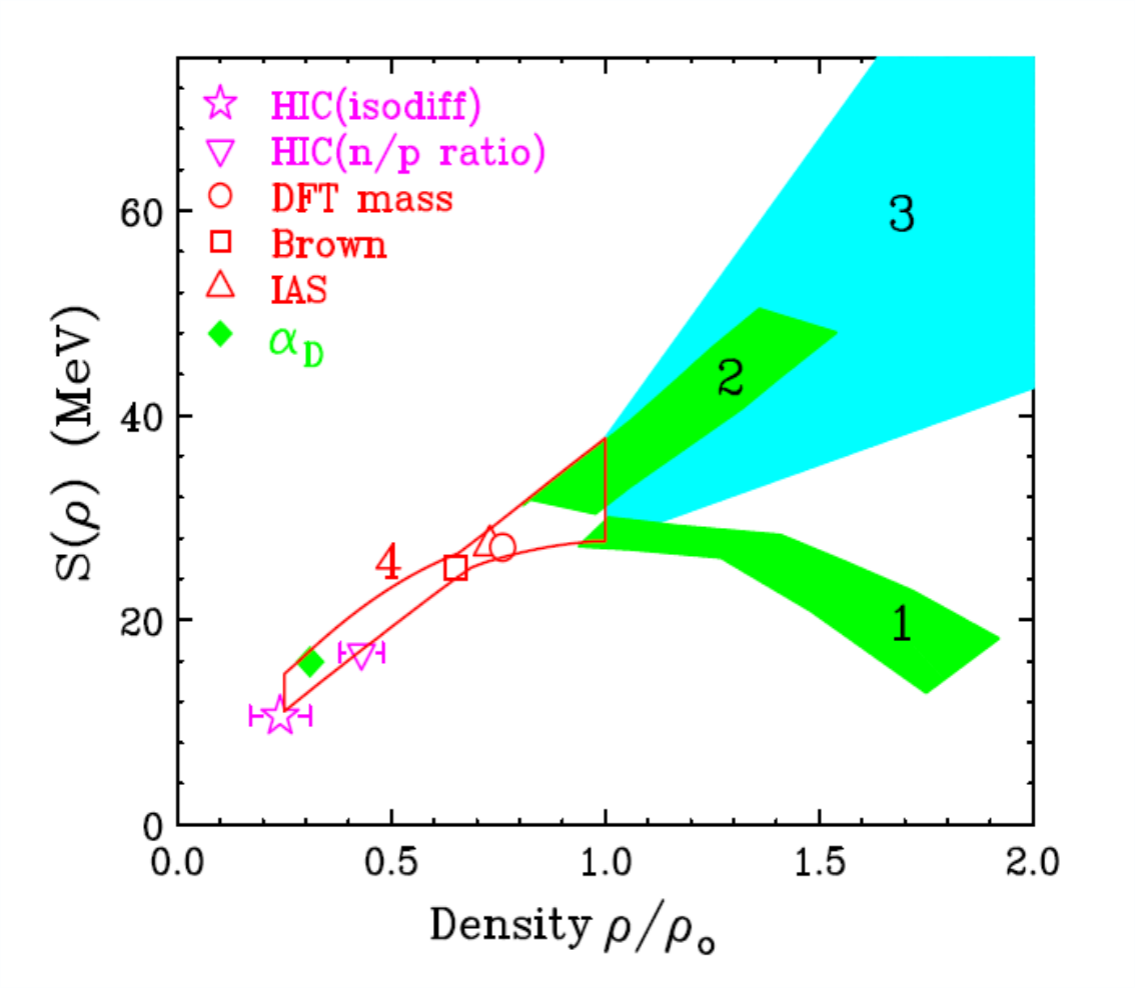
\includegraphics[scale=.3]{densityDep.png}
\caption{Current experimental constraints on the density dependence of the symmetry energy. The measured data points are discussed in the text. The 4 polygonal and shaded regions are constraints from: 1.) pion analysis from Ref. \cite{xia2009,xie2013}, 2.) a separate pion analysis from Ref. \cite{feng2010}, 3.) ASYEOS experiment \cite{russo2011, russo2016, cozma2013} and 4.) isobaric analog states \cite{dan2014} }
\label{fig:symDen}
\end{figure}

In the last couple decades, the symmetric term of Eq.~\ref{eq:energyEos} has been determined for a wide range of densities ranging from $\rho_0 - 4.5\rho_0$ \cite{scienceEos}. In contrast, the symmetry energy has only been accurately constrained for densities at or below $\rho_0$ and only preliminary constraints have been obtained at higher densities. Figure~\ref{fig:symDen} shows the current status of laboratory constraints on the density dependence of the symmetry energy. The red region labeled 4.) for $\rho < \rho_o$, corresponds to constraints from isobaric analog states \cite{dan2014}. Notice that the symmetry energy is consistent across  a series of independent measurements and observables, but not at higher densities \cite{awayforward}. At higher densities, the two green sections correspond to constriants obtained from total pion yields, and the total pion ratio $\pi^-/\pi^+$, from Au + Au collisions at various beam energies \cite{fopi}. Region 1.) is obtained from analysis performed in References~\cite{xia2009,xie2013} while Region 2.) corresponds to Reference~\cite{feng2010}, giving conflicting results from the same data set. The blue shaded region (labeled 3.) corresponds to constraints obtained through proton and neutron elliptical flow reported in References~\cite{russo2016,cozma2016,cozma2017}. There is still a considerable uncertainty in the symmetry energy at high densities, which are more relevant to neutron stars. It has been the goal of the nuclear EoS community over the last decade to constrain the symmetry energy at these high densities. 




\section{Heavy Ion Collisions}
Besides observing neutron stars directly, heavy-ion collisions (HIC) provide the only way we can probe the density dependence of the symmetry energy in the laboratory setting. When two nuclei collide, in the very early stages they compress to form a high density region where the nuclei overlap. This momentary density can reach up to $3\rho_0$ ,depending on the incident beam energy, over a small volume where the nuclei overlap.  HICs also provide the only way we can probe the isospin asymmetry dependence of the nuclear EoS. This is accomplished by using radioactive neutron-rich beams to collide on stable targets. 

The pressure arising from the symmetry energy depends on the curvature of the symmetry energy at a given density as described in Eq.~\ref{eq:densEos}. If the density dependence of the symmetry energy grows with a positive derivative at high densities, the symmetry energy would in general force neutrons out of the high density system. If the symmetry energy decreases at high densities, making the derivative  negative, then the symmetry energy term would tend to attract neutrons. The symmetry energy is referred to as \emph{soft} if the second order term in the Taylor expansion -- at saturation density-- is negative, and \emph{stiff} in the case of a curvature that is close to zero or positive. It is the pressure coming from the symmetry energy that is driving the relative dynamics of neutrons and protons, where a stiff symmetry energy expels neutrons from dense matter and expels them less for a softer symmetry energy.

By measuring protons and neutrons, we can see signatures of the symmetry energy in the final spectra of these particles. There are two experimental challenges. First,  measuring neutrons precisely can be quite challenging. The existing technology of neutron time of flight arrays requires long flight paths and large, inefficient detectors. Inevitably, the acceptance is limited by cost and the space required for large neutron wall arrays. Lastly, though the overlap region of the two nuclei temporarily reaches a high density, the nucleons which participated in this region continue to evolve throughout the collision, even into regions of lower densities until they reach their final state. They are continuously interacting with the rest of the nuclear matter, covering a wide range of densities, which dilutes any information about the symmetry energy at at high densities.  




\section{Pion Observable}
\label{sec:pionObs}
Another approach is to find an observable that can be detected with high efficiencies, unlike the neutron, and is more sensitive to just the high density region. For these reasons pions are a very interesting observable. Pions are produced through an intermediate step via production of $\Delta$ resonances. Here the reaction $ NN \leftrightarrow \Delta N$ takes place, where nucleon-nucleon collisions form $\Delta$(1232) baryon resonance from one of the nucleons, which then decays shortly thereafter into a pion and nucelon, $\Delta \leftrightarrow \pi N$. The threshold for  an on-shell $\Delta$ resonance production in nucleon-nucleon collisions, with a mass of \SI{1232}{\mega\electronvolt\per\clight\squared}, corresponds to a laboratory beam of \SI{290}{\MeVA} in a fixed target experiment. In large nuclei, the internal motion of the nucleons is substantial and this modifies the production rates. In the Fermi gas model, nucleons are arranged filling up higher energy levels up until they reach the Fermi energy. The associated Fermi velocity can add to the beam velocity and actually be above the threshold condition, even when the beam velocity is below the threshold \cite{fermiEnergy}.


Nuclear collisions are typically calculated via semi-classical theories based on a extension of the Boltzmann equation or by modifications of molecular dynamics \cite{bertsch}. These theories predict that most of the $\Delta$'s are produced in the early, dense regions of the collision \cite{mingzhang}. Panel (c) of Figure~\ref{fig:deltaProduction} shows the average local density where $\Delta$'s are produced, and the total  number of $\Delta$'s produced in the system (b), as a function of time in the simulation, for Au + Au collisions at \SI{400}{\MeVA}. Panel (a) shows the distribution of density at moment of creation for each $\Delta$. Since the average lifetime of the $\Delta$  is $\tau_{\Delta} = \SI{1.7}{\femto\metre\per\clight}$, the $\Delta$ resonance has very little time to be affected by the medium before decaying into a $\pi$ and nucleon. Thus the outgoing $\pi$ can contains information on the high density region of the collision. 

\begin{figure}[!htb]
\centering
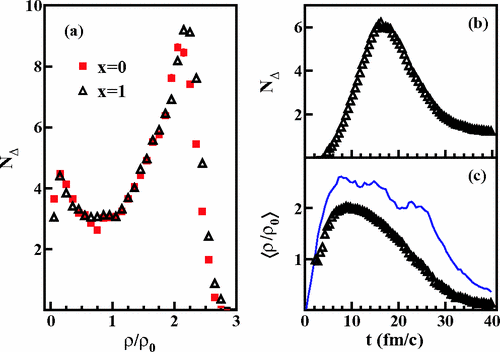
\includegraphics[width=.6\textwidth]{deltaProduction.png}
\caption{Figure taken from \cite{mingzhang} for Au + Au collisions at \SI{400}{\MeVA}. Panel (a) shows the density in the region of the $\Delta$ resonance creation for two different symmetry energies (x=0 soft) and (x=1 stiff). Panel (b) and (c) show the evolution of collision in time steps, where (b) shows the number of deltas in the system as a function of time and (c) shows the mean local baryon density in the region where $\Delta$ resonances are produced. The blue line in (c) represents the average baryon density in the most central region of the collision. This evidence shows that a majority of $\Delta$'s are produced in the high density region of the early collision.}
\label{fig:deltaProduction}
\end{figure}

The branching ratio of the various flavors of $\Delta$'s are given by the Clebsh-Gordan coefficients as shown in Appendix~\ref{appen:deltadecay}. Here we see that in general proton-proton collisions give rise primarily to  $\pi^+$ and neutron-neutron collisions give rise to primarily $\pi^-$. From these branching ratios the charged pion ratio can be described as,

\begin{equation}
\frac{\pi^-}{\pi^+} = \frac{ 5N^2 + ZN }{5Z^2 + ZN}.
\label{eq:deltaModel}
\end{equation}

In this simple $\Delta$ resonance model, $\pi^-/\pi^+ \approx (N/Z)^2$ where $N/Z$ is the neutron-proton ratio of the dense central collision where they are produced. Pions can be reabsorbed into a $\Delta$ resonances after colliding with another nucleon in the backward process of $\Delta \leftrightarrow \pi N$, only to be re-emitted again into a pion. This process generally dilutes the pion sensitivity to the high density region, since with each absorption and re-emission changes the pion dynamics or even the charge of the pion reflecting the neutron-proton asymmetry at the point of creation and re-emission. Total pion absorption, going back into two nucleons, requires a three body process; i.e. the pion collides with a nucleon creating a $\Delta$ resonance, then another nucleon must quickly collide with the resonance to create two nucleons. Since this is a three body process, the total pion absorption (removing them from the system) is a smaller effect than the absorption and re-emission process. Aside from these two effects which degrade the observable, in general the $\pi^-$ are connected with neutrons and the $\pi^+$ production with proton behavior in the high density, early collision; effectively turning the problematic neutron into a measuring charged $\pi^-$ , which is much easier to measure experimentally. It is also directly related the high density region where the $\Delta$'s are produced.  

\section{Motivation}
In an effort to answer the high density behavior of the symmetry energy, we designed a new detector and a set of experiments of Sn + Sn collisions at \SI{270}{\MeVA}. Here we utilized inverse kinematics where the beam is made of a radioactive neutron rich beam, impinging on a stable Sn target. We can probe the isospin asymmetry of the symmetry energy by changing the neutron-proton asymmetry of the incoming beam. Pion production has been studied before in stable beams for beam energies of \SI{400}{\MeVA} and above \cite{fopi}. Yet in these previous experiments, only the total pion yields were published and not the pion spectra. It was also known that the efficiency analysis of the FOPI collaboration \cite{fopi} which was particularly difficult especially for low energy pions. In fact the published pion multiplicities are not the measured values but rather extrapolated to low pion energies. We know now that below the FOPI cutoff cited in \cite{fopi}, approximately 35\% of the $\pi^+$ multiplicity and 55\% of the $\pi^-$ multiplicity, showing the importance of measuring down to low pion energies. While the pion production increases with the beam energy, this increase is countered by the fact that the effects of the symmetry energy decrease with energy \cite{fopi}. This is because available energy to produce pions is larger and therefore less sensitive to the relatively small symmetry energy.  The goal of this Dissertation was to design and build a high efficiency detector in order to measure pion and light charged particle spectra resulting from HICs. To do this a new Time Projection Chamber (TPC) was made called the SAMURAI pion Reconstruction Ion Tracker (\spirit) TPC.

\section{Dissertation Outline}
In this dissertation we will begin with a discussion of the operating principles of the \spirit TPC and the general setup of the experiment in Chapter~\ref{chap:experiment}. We will then talk about the corrections and calibrations applied to the data, as well as a brief introduction into the software and analysis procedure in Chapter~\ref{chap:data1}. This will naturally lead into a discussion in Chapter~\ref{chap:data2} about the various quality cuts taken on the data to improve the background rejection improving the signal to background ratio; this will also include the particle identification technique used to extract the pions. Finally in Chapter~\ref{chap:results} we will present the extracted pion yield, ratios, and spectra for the neutron-rich  $\tin{132}{124}$ system, and the neutron-poor $\tin{108}{112}$ system; which complement the systems analyzed in the dissertation by Jonathan Barney \cite{jon}. In Chapter~\ref{chap:summary} we will give a summary of the results and an outlook towards constraining the symmetry energy at high densities using pions. 
\chapter{Experiment}
\label{chap:experiment}

A Time Projection Chamber (TPC) is a detector that reconstructs the energy loss of charged particles and the location of that energy loss as in all 3 dimensions within the detector. TPCs have been employed in gases, liquid, and even solid detectors \cite{starTPC,arTPC,eosTPC}. In the following, we outline the physical principles involved in measurements within a gaseous TPC, and discuss the particular details of the TPC used in this Dissertation, along with the rest of the experimental setup.


\section{Operational Principles of Time Projection Chambers}

%explain in breif the basics of a time projection chamber 
\begin{figure}[!htb]
\centering
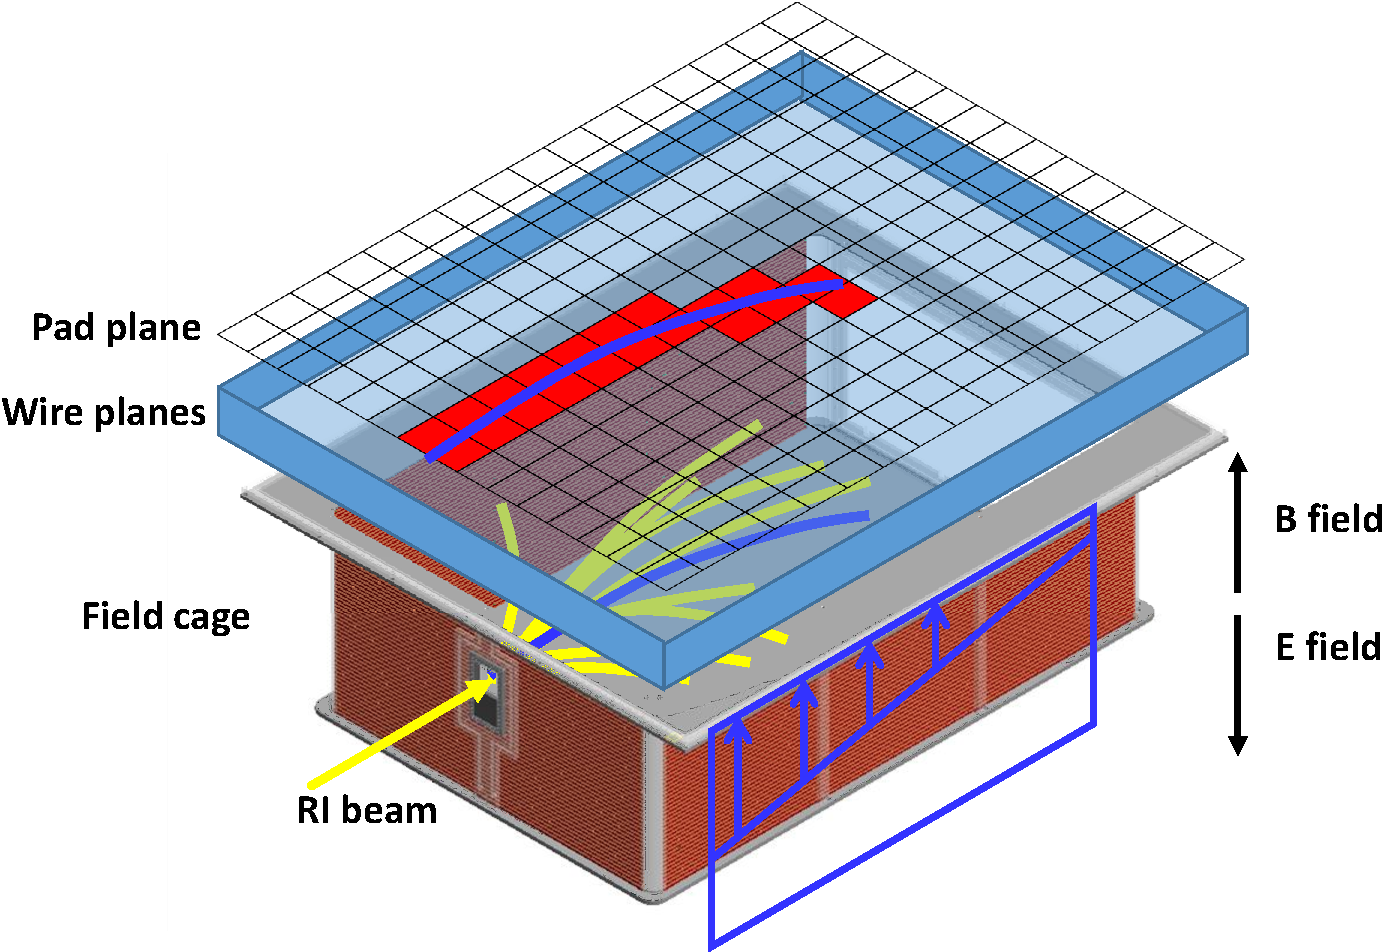
\includegraphics[scale=.5]{tpcPrinciple.pdf}
\caption{Cartoon depicting the operating principles of the TPC is.}
\label{fig:tpcPrinciple}
\end{figure}

%explain in breif the basics of a time projection chamber 
Figure~\ref{fig:tpcPrinciple} depicts the interior of a gaseous TPC and its field cage. The field cage holds the detector gas and also defines a constant electric field that is typically aligned with the magnetic field of a magnet that surrounds the TPC. In this Spirit TPC, both these electric and magnetic fields are vertical.  

As a charged particle resulting from a heavy ion collision passes through the field cage, energetic \emph{primary} electrons are knocked out of neutral gas molecules and atoms in the detector gas. These primary electrons further ionize the detector gas until there is a distribution of \emph{secondary} electrons and positive ions that lie along the track's path. The electric field of the field cage separates these electrons and ions, where the electrons are accelerated upward by the electric field in the direction against the electric field, and the positive ions are accelerated along the electric field. Since the mean free path of the electrons inside the gas is very small, they quickly collide with other gas molecules, which slow down, or even stop the electron; only to be re-accelerated by the electric field, continuing a repeating cycle of stop and go motion. This microscopic behavior results in a constant drift velocity when averaged over multiple gas collisions. 

The electrons drift with this drift velocity through a set of wire planes, eventually reaching a set of high voltage anode wires, where they quickly accelerate in the presence of the high electric field emanating from the anode wires. This high electric field imparts enough energy between collisions to ionize the gas, creating additional electron-ion pairs from the gas, culminating in an avalanche process near the anode wires. The avalanche electrons typically terminate on the anode wire,  while the ions created in the avalanche are accelerated  away from the anode wires. This ionic motion induces image charges in nearby pads within the pad plane that is located close to the anode wires. The corresponding image currents in these pads are read out by electronics that are attached to these pads. This electronics signal encodes the energy loss information and arrival time of the signal from the electrons drifting from the ion track, and can be analyzed to determine the position of the ion track within the TPC. 

The pad plane is perpendicular to the electric field of the field cage and is divided into a two dimensional grid of pads. Two of the 3 coordinates are determined from the 2-dimensional charge distribution corresponding to the projection of the track onto the pad-plane. The third dimension comes from extrapolating the electrons back in time, utilizing the known constant drift velocity $v_d$. The distance the electron has traveled , $d$, -- along the electric field direction-- is calculated as $d = v_d \cdot t$, where $t$ is the drift time information obtained from combining the time of the event trigger with arrival time of the signal from the  electrons in the electronics. The radius of curvature of the track on the pad plane is related to the magnetic rigidity, and therefore the momentum of each track. The energy loss deposited $\langle dE/dx\rangle$ is proportional to the image charge induced on the pads on the pad-plane. With these two observations, particles can be uniquely identified by their mass and charge since there is a unique correlation between the rigidity and $\langle dE/dx\rangle$  lines. This correlation allows the particle type to be identified as discussed later in Section~\ref{sec:pid}. In this chapter we will provide more details about the particle detection within the \spirit TPC  that is relevant to the reactions studied in this Dissertation. 


\section{S$\pi$RIT TPC Overview}
%Add Overview image with labels

\begin{figure}[!htb]
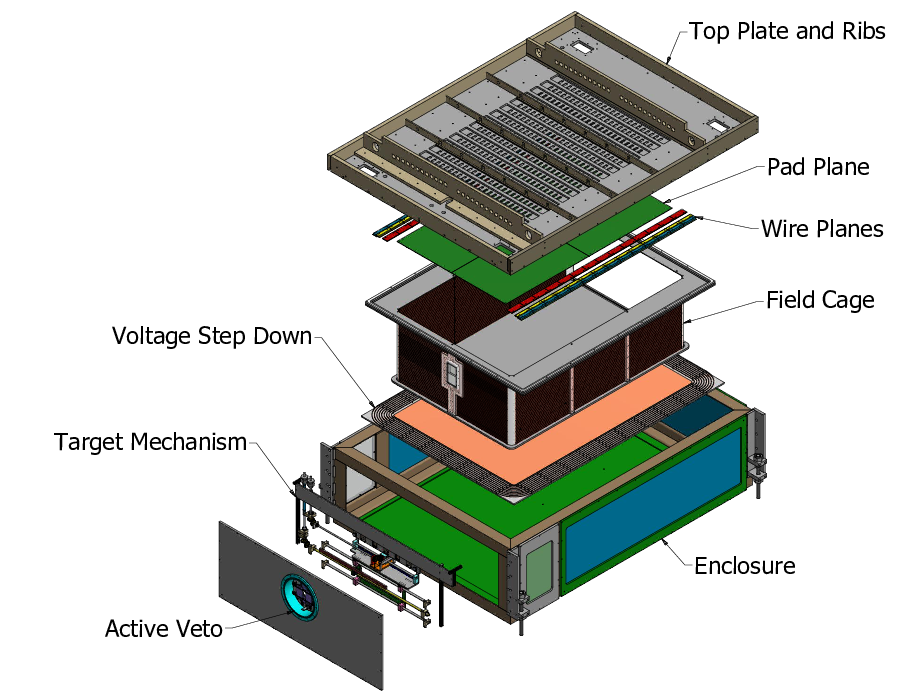
\includegraphics[width=\textwidth]{exploded.png}
\caption{Exploded overview of the of the \spirit TPC}
\label{fig:tpcExplode}
\end{figure}


The SAMURAI Pion-Reconstruction and Ion Tracker Time Projection Chamber (\spirit TPC) was developed to measure pions and other light charged particles produced in collisions of radioactive rare isotope beams with stable targets in fixed target experiments.  The TPC is built on an Aluminum angle iron skeleton with thin Aluminum sheet walls in order to minimize neutron scattering and to allow for light charged particles to reach auxilliary detectors on the sides and downstream of the TPC. The \spirit TPC was developed to fit inside the SAMURAI dipole magnet used at the Rare Isotope Beam Factory (RIBF) at RIKEN in Wako-shi, Japan \cite{riken}. The dipole gap limited the vertical space of the TPC to around \SI{75}{\centi\metre}. More detail and specifications of the SAMURAI dipole magnet are given in \cite{samurai}. 

The exploded drawing shown in Fig.~\ref{fig:tpcExplode} illustrates these major internal components of the  of the \spirit TPC. A target mechanism allowed for up to 5 fixed targets to be mounted on the target ladder situated just upstream of the field cage, where changing the targets could be performed outside of the magnet. Reaction products from nuclear collisions exit the target and enter the field cage of the TPC. The field cage contains the detector gas and defines the constant electric field. It is rigidly mounted to the large Aluminum top plate of the TPC enclosure. The field cage is electrically isolated from the top plate by a lexan top perimeter ring with o-rings to provide as gas seal. The pad plane and wire plane structures are  mounted to the inside face of the top plate with the electronics being mounted on the outside face of the top plate. Several Aluminum ribs were also mounted to provide extra rigidity to the top plate, keeping it flat to within \SI{150}{\micro\metre}, as measured by a precise laser measurement \cite{jon}. Holes in the top plate allowed signals from the individual charge sensitive pads on the pad plane to be transmitted via cables to the electronics. 



\begin{table*}\centering
\ra{1.3}
\begin{tabular}{@{}rr@{}}\toprule 
\multicolumn{2}{c}{\spirit TPC Overview} \\
 \midrule
Pad plane area & 1.3 m x .9 m\\
Pad size       & 1.2 cm x .8 cm \\
Number of pads & 12096 (112 x 108) \\
Gas composition& 90\% Ar + 10\% CH${}_4$ (1 atm)  \\
Multiplicity limit & 200  \\
dE/dx range        & Z=1-3, $\pi$, p, d, t, He, Li \\
Drift length       & 50 cm \\
\bottomrule
\end{tabular}
\caption{Summary of general properties of the \spirit TPC.}
\label{tb:spiritoverview}
\end{table*}


\begin{comment}
\subsection{Enclosure}
The skeleton of the enclosure is composed of a rigid rectangular Aluminum angle-iron frame. To this frame, six rectangular sides are attached. The downstream window and the two side windows are constructed of a Aluminum window frames with a 1 mm  Aluminum sheet metal window. These thin sheet metal windows allow charged particles and neutrons to exit the TPC without significant energy loss or scattering. This allows for a trigger to be created by placing detectors outside of  the side windows and downstream window of the TPC. The enclosure itself is made to be gas tight with no leakage from the outside or from the interior of the field cage. This is to allow for the possibility to choosing one insulation gas outside of the field cage and a different counter gas inside the field cage. In the first campaign of experiments, however, we used the same gas in the field cage and enclosure volume.  
\end{comment}

\subsection{Field Cage}
%The field cage contains the detector gas and defines a uniform electric field in which electrons can drift upwards toward the anode wires. It was designed to hang from the top plate and therefore needed to be of a lightweight construction and the materials needed to be thin to allow for light charged particle and neutrons to pass through to ancillary trigger detectors without significant energy loss or scattering .  

\begin{figure}[!htb]
\centering
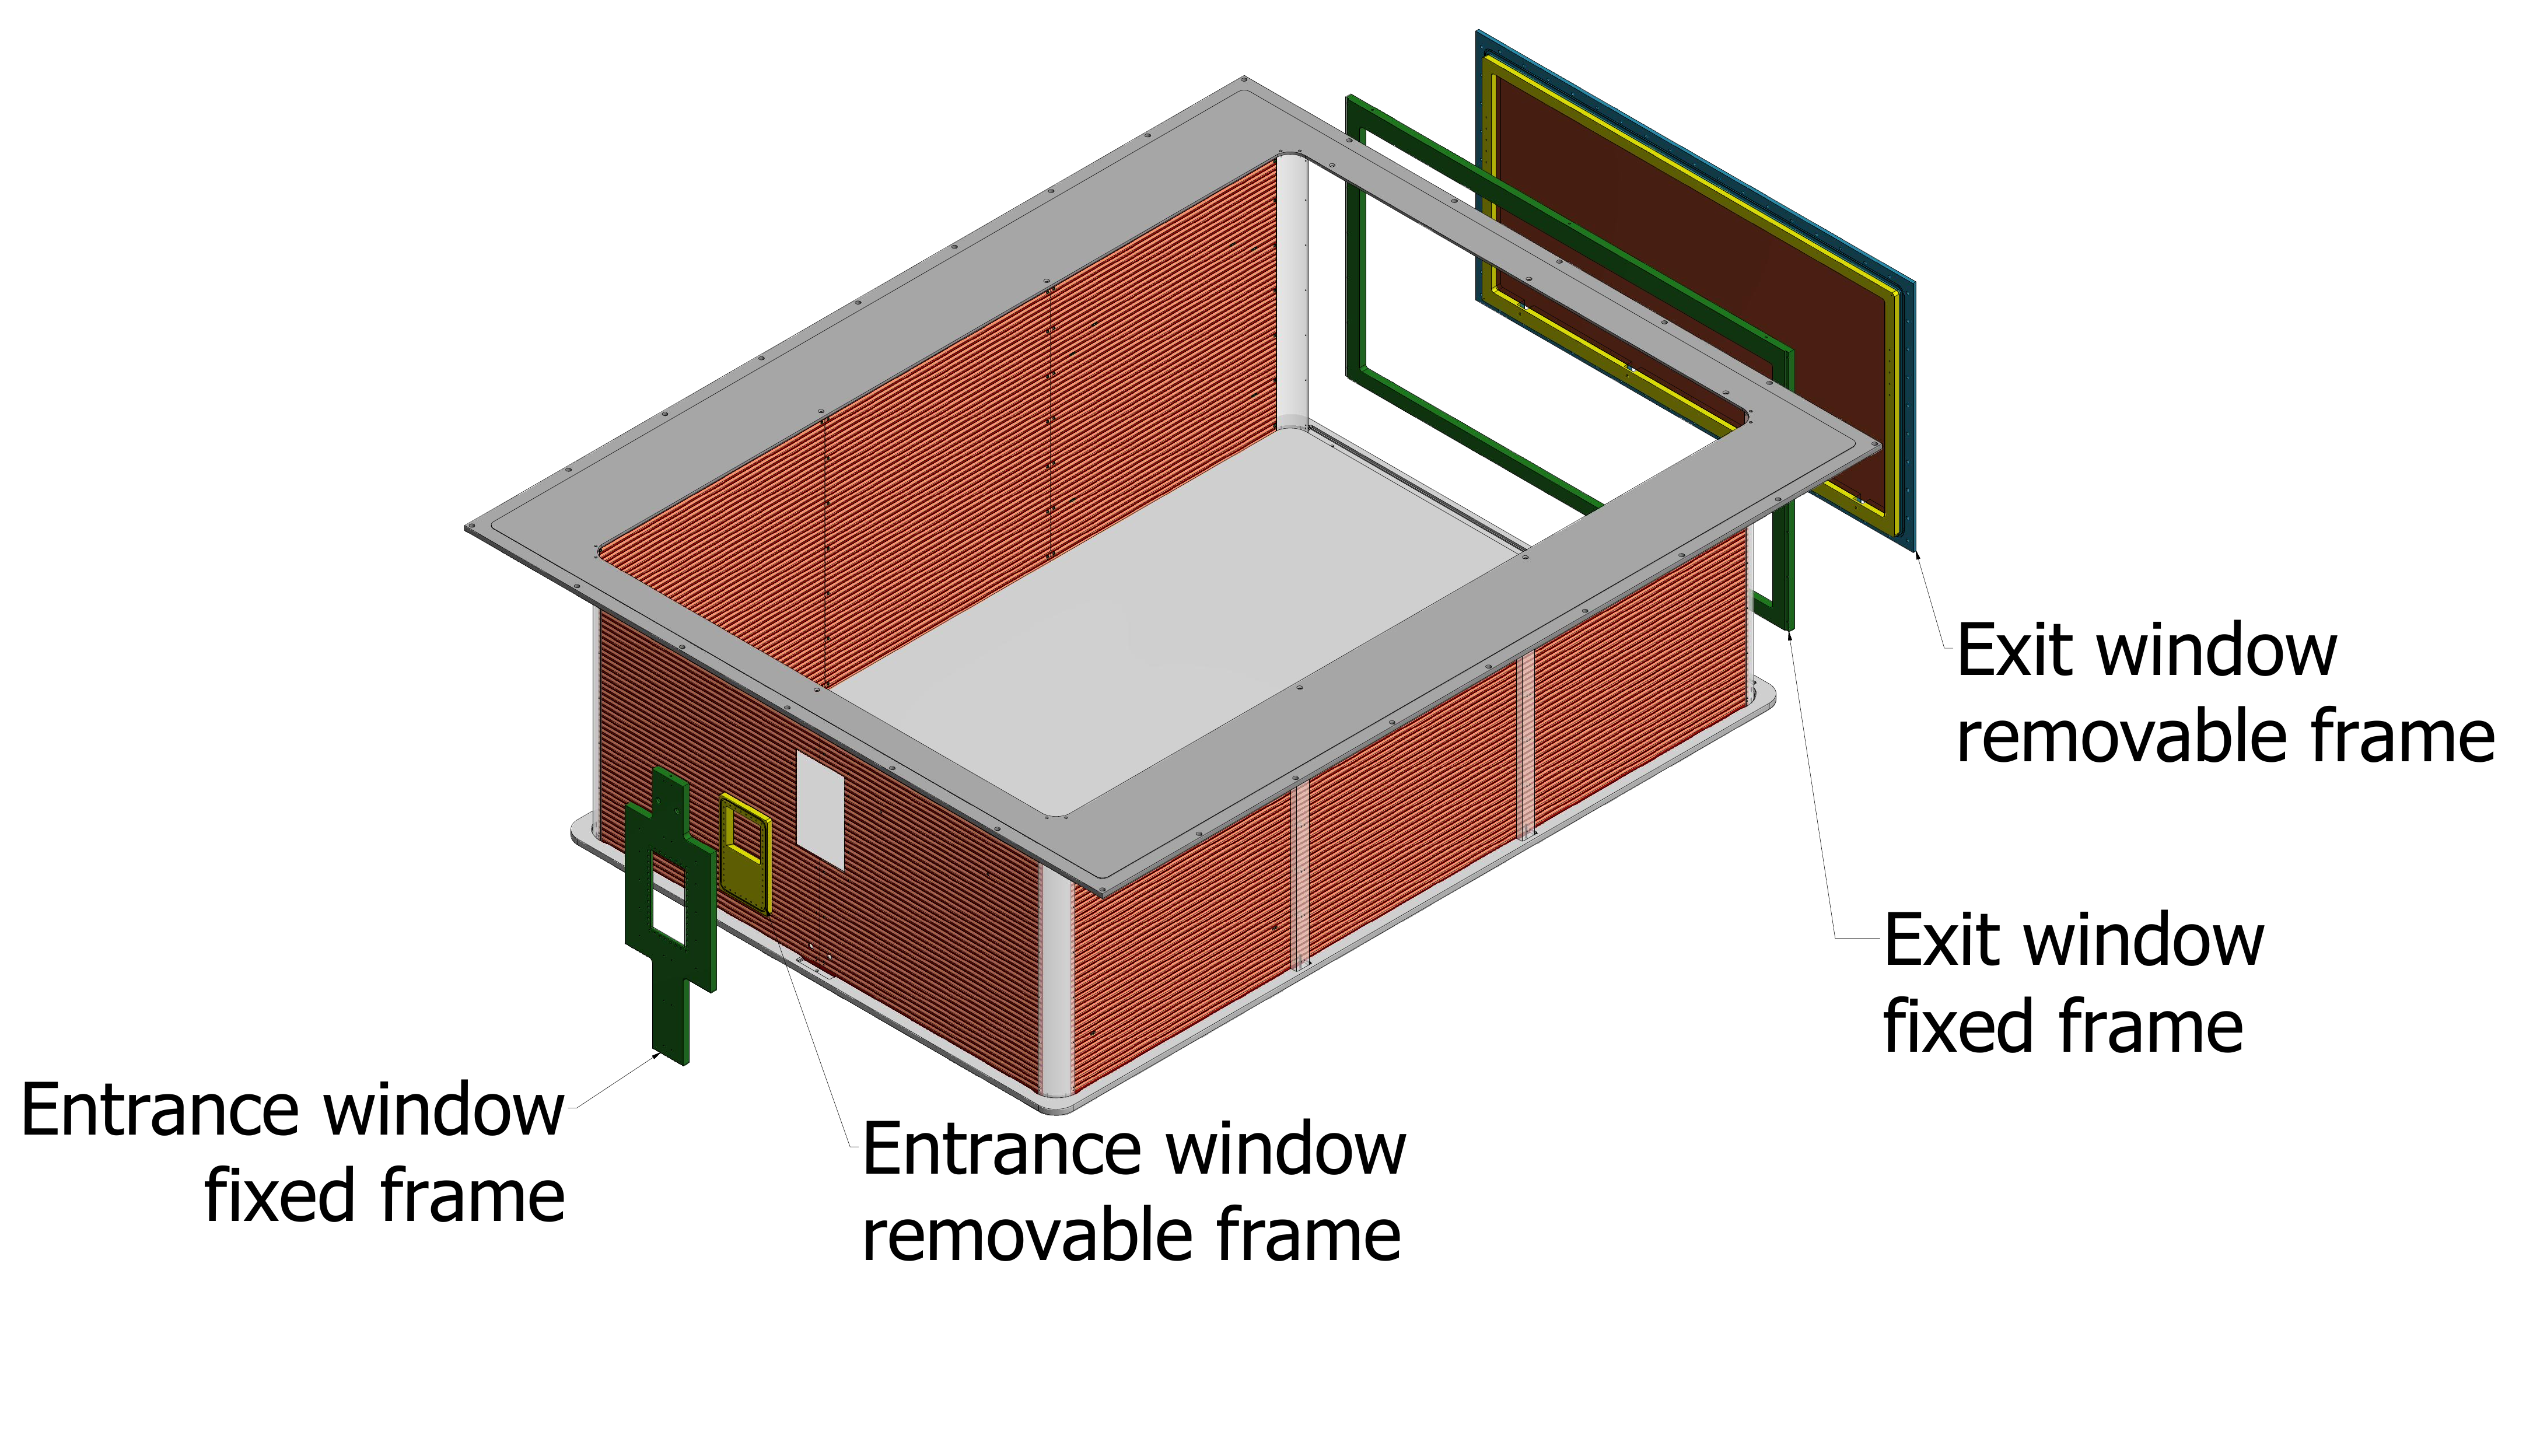
\includegraphics[width=.9\textwidth]{fc_overview.png}
\label{fig:fc_overview}
\caption{Overview of the field cage mechanical components.}
\end{figure}


\begin{figure}[!htb]
\centering
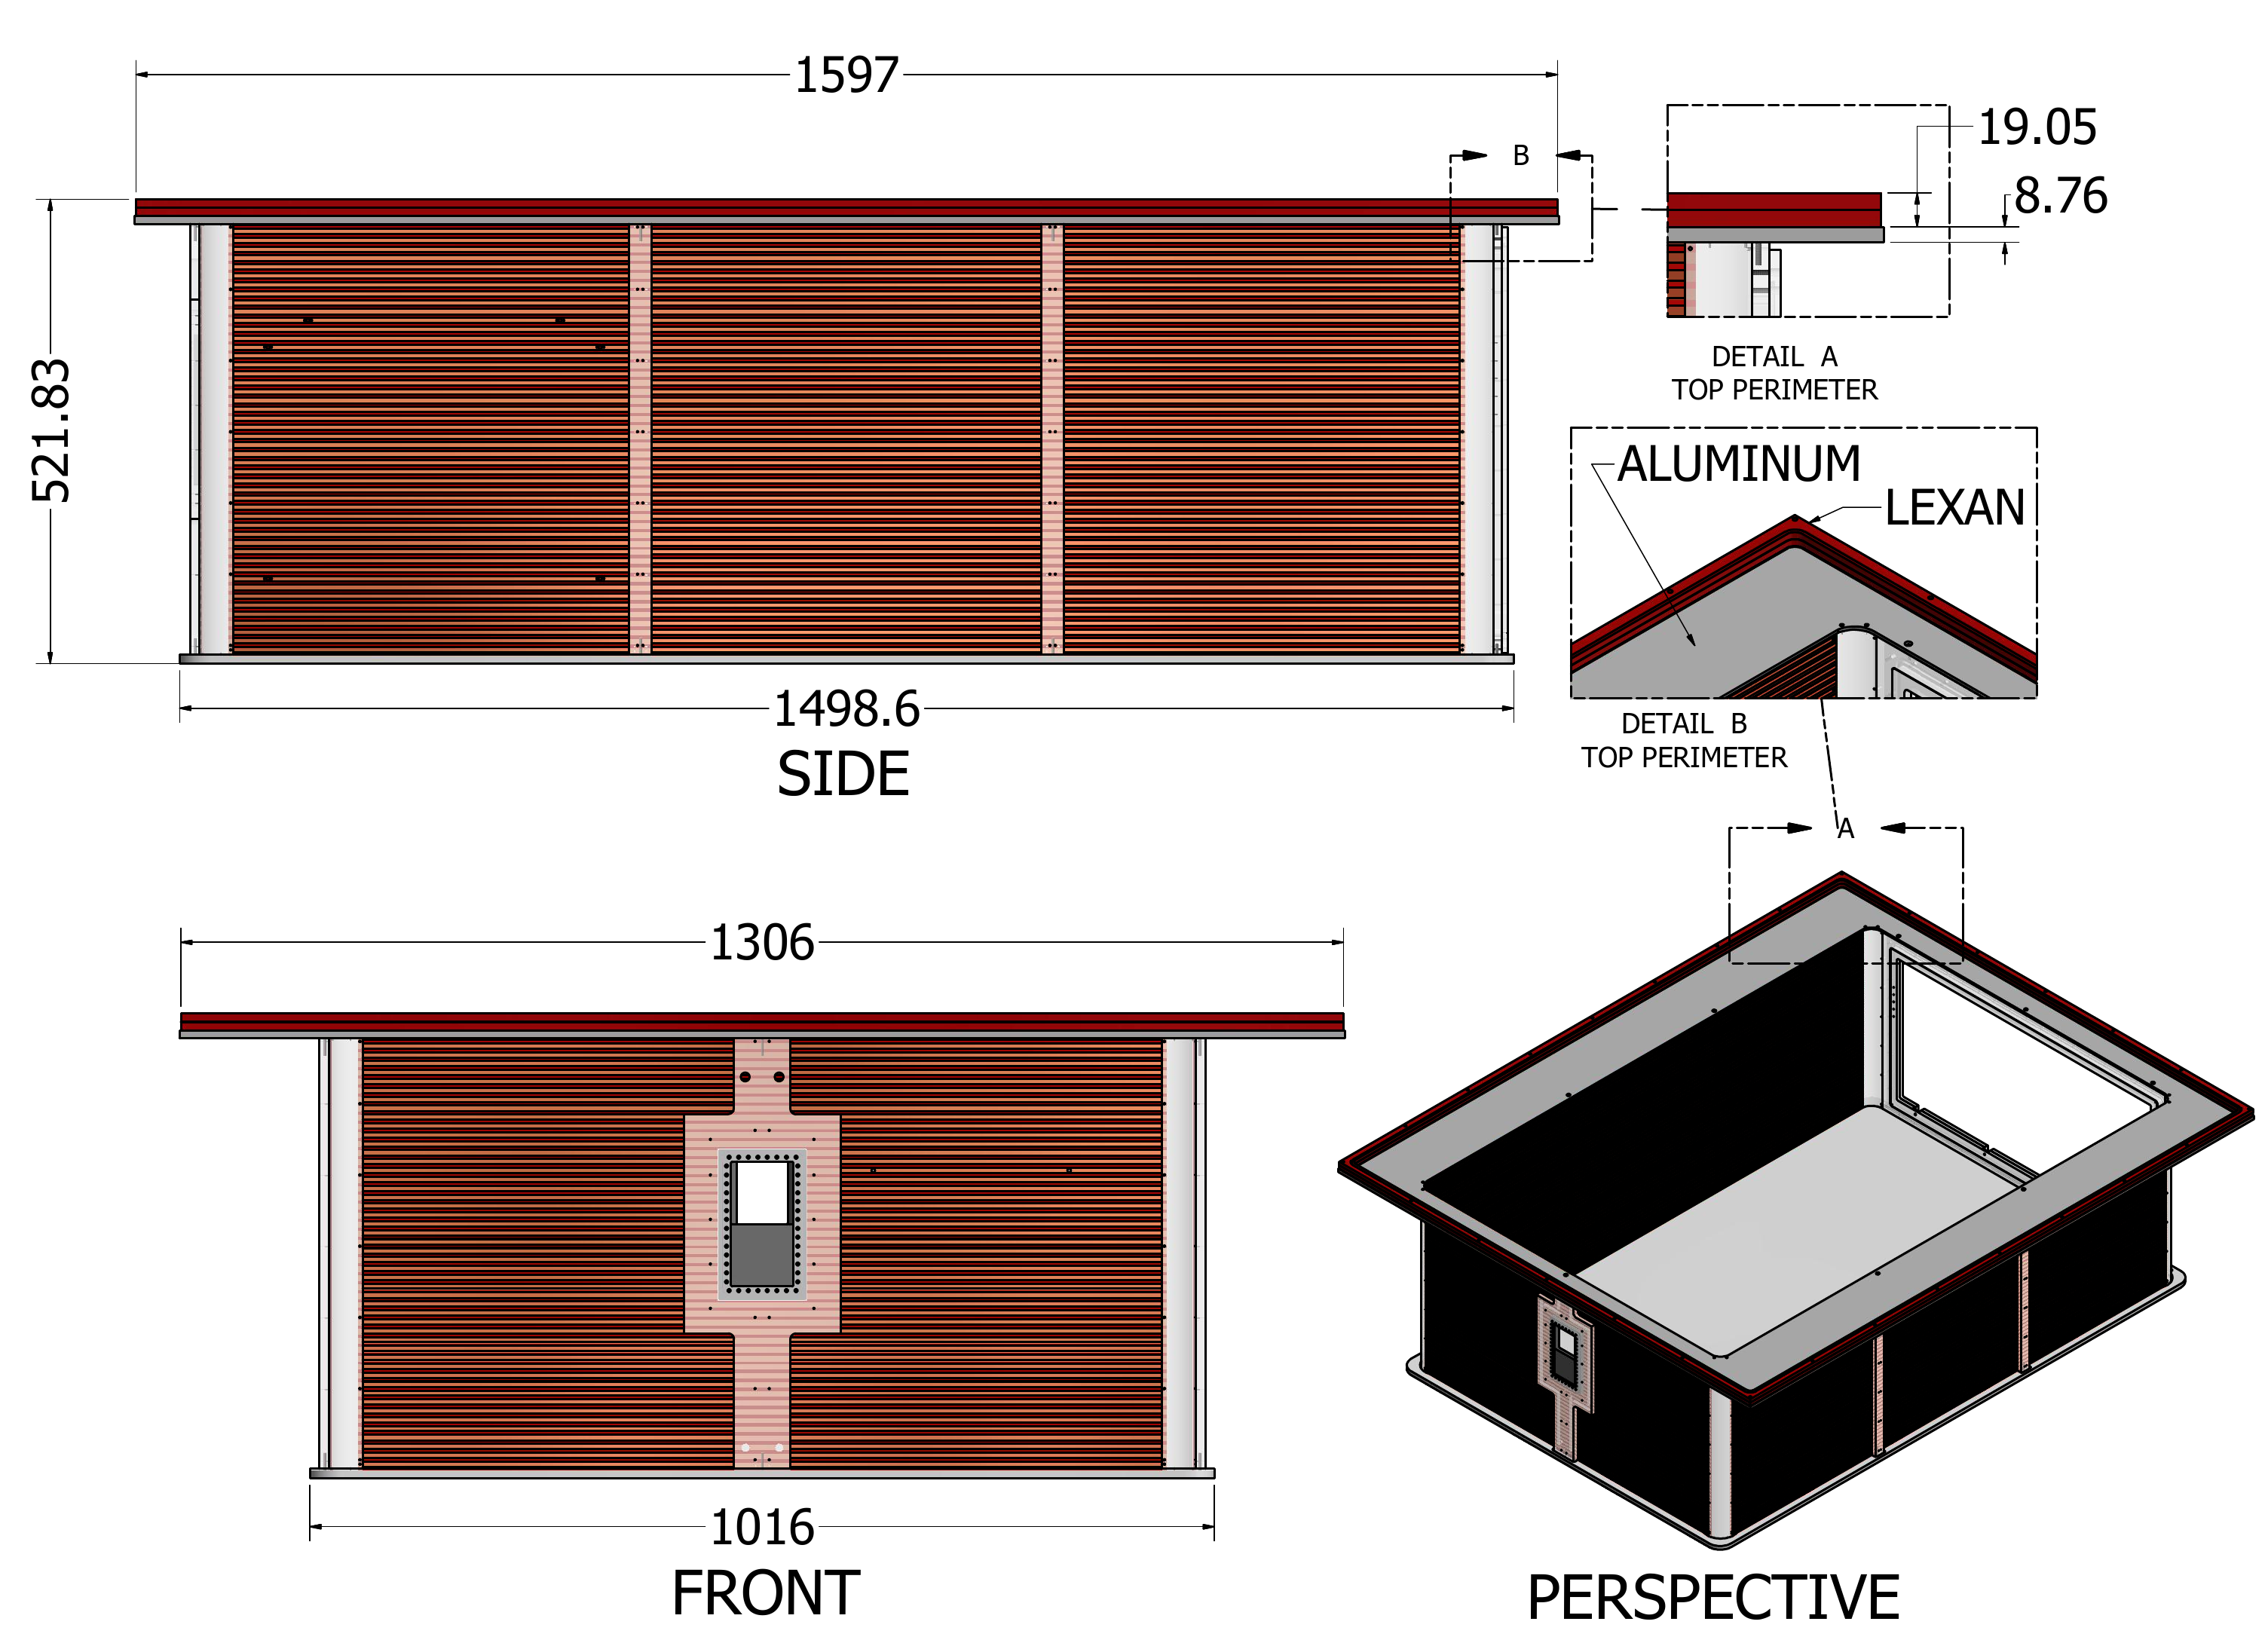
\includegraphics[width=.8\textwidth]{fc_overview2.png}
\label{fig:fc_overview2}
\caption{Schematic of the field cage.}
\end{figure}


The field cage was constructed from several panels of two-layer printed circuit board (PCBs). The front of the field cage was made of two PCBs and each side was constructed from three PCBs. These boards had copper strips etched onto the inside and outside of the board which when all the boards were assembed, formed copper rings which were used to set up the uniform electric field, as will be described later. The array of circuit boards were glued and supported by Lexan pieces. We did not use the common PCB substrate material FR4, which contains a Bromine impregnated epoxy which can outgas Bromin and absorb the secondary electrons from the track, thereby degrading the signal \cite{tpcAging}. Instead, a halogen free material, Cryogenic-G10, was used for the board material.  The downstream wall mainly consists of a large, thin exit window. The window  is constructed of   \SI{10}{\micro\metre} Kapton upon which are  evaporated Aluminum strips that define the electric field. At the bottom of field cage is the cathode that is  constructed from an Aluminum honeycomb laminate, composed of two Aluminum sheets bonded to an Aluminum honeycomb core, providing a lightweight yet rigid structure. On the other end the boards were epoxied into an Aluminum top perimeter which also served as the last electrode ring in the TPC. Together with the cathode bottom, the field cage proved to be a rigid lightweight structure. A Lexan ring containing o-rings was placed in-between the top perimeter piece and the top plate of the TPC. Screws with nylon washers, and collars, were used to mount the top perimeter, and the field cage, to the top plate; it also provided electrical isolation from the top plate. In this way the top plate could be removed and rotated with the field cage attached, without damaging any internal components. 

\begin{figure}[!htb]
\centering
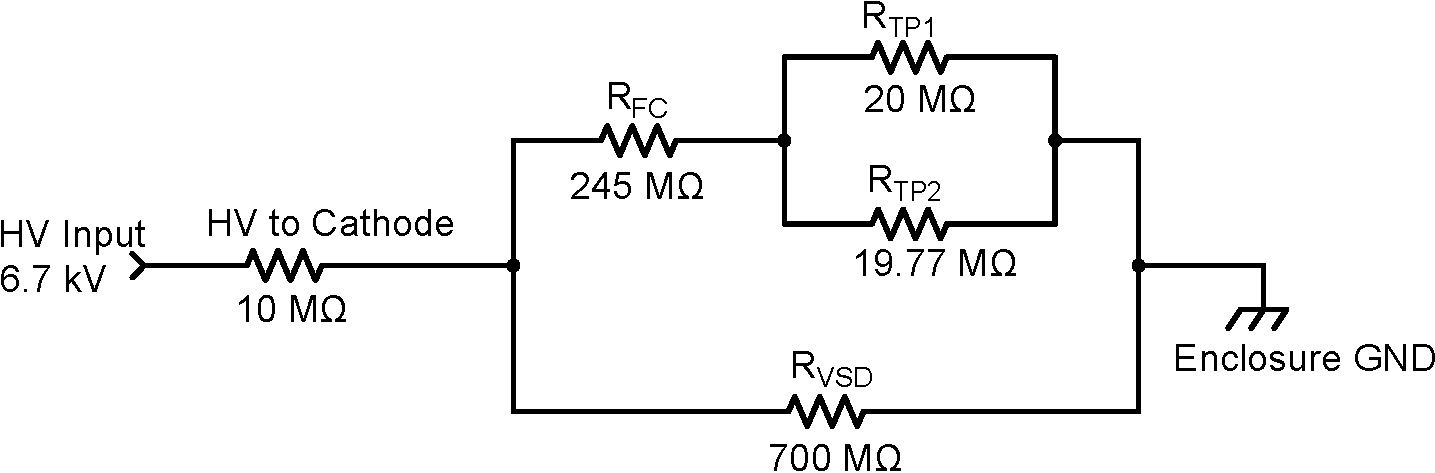
\includegraphics[width=\textwidth]{TPC_schematic.pdf}
\caption{Schematic of the resistive elements in the TPC system.}
\label{fig:TPC_schematic}
\end{figure}



Figure~\ref{fig:TPC_schematic} shows the schematic of the effective resistances of the TPC subsystem. The cathode is connected to the high voltage (HV) supply through a \SI{10}{\mega\ohm} resistor and has an effective capacitance to ground of \SI{4}{\nano\farad}, $C_{VSD}$. The cathode voltage $V_{cath}$ can be calculated as,
\begin{equation}
V_{cath} = \frac{V_{HV}}{ 1 + \frac{10}{ \left( (245 + R_p)^{-1} + 700^{-1} \right)^{-1} } },
\end{equation}
where 
\begin{equation}
R_p = \left( R_{TP1}^{-1} + R_{TP2}^{-1} \right)^{-1},
 \label{eq:Reff}
\end{equation} 

is the effective resistance of the last resistor, and $V_{HV}$ is the high voltage supply; all resistor values are given in \si{\mega\ohm}.


\begin{figure}[!htb]
\centering
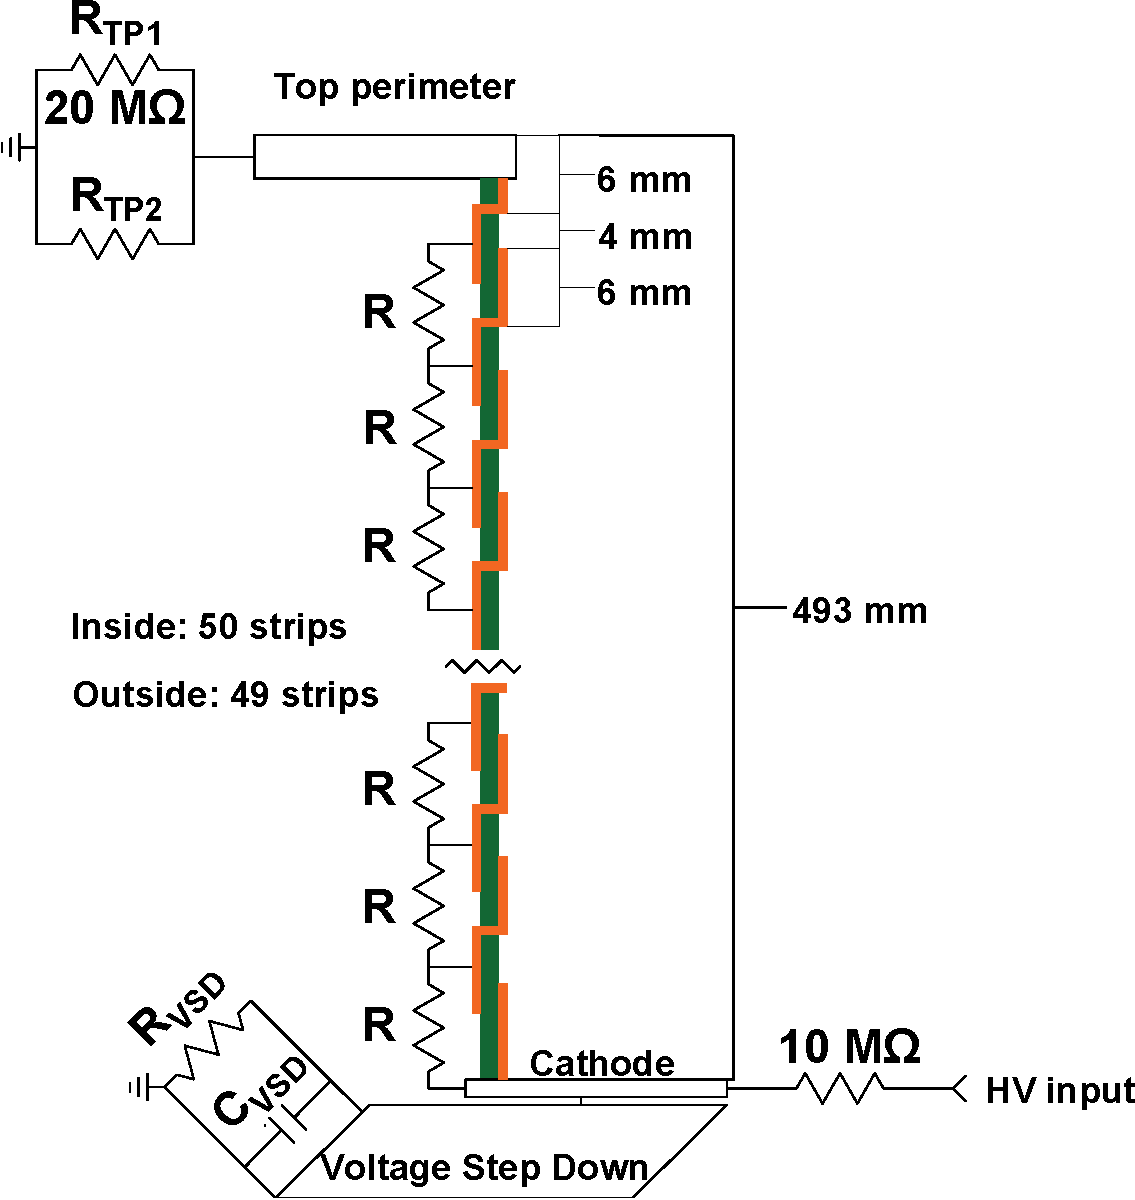
\includegraphics[scale=.6]{FC_schematic.pdf}
\caption{Schematic of the electric connections relevant to the field cage system. The strip thickness is exaggerated in the figure to show the detail.}
\label{fig:FC_schematic}
\end{figure}

Figure~\ref{fig:FC_schematic} shows a schematic detailing the connections involved in the field cage walls. The field cage contains 50 inside copper strips and 49 outside copper strips. The strips are \SI{6}{\milli\metre} in width and spaced \SI{10}{\milli\metre} apart. Since the field cage was built with an array of PCB boards, connections from adjacent strips were connected all the way around until all the strips formed a continuous ring. The interfaces where the side pieces met were connected by G10 corner pieces where conductive paint strips were painted on. The first inside strip is connected to the cathode, which is itself connected by an effective \SI{5}{\mega\ohm} resistor ($R$) to the first outside strip. The first outside strip is connected through a via to the second inside strip. These outside strips formed a small electric field which repelled electrons away from the PCB substrate between inside strips, preventing build up on the insulating material. This pattern repeats until the very last strip. A resistor chain, connected to the outside strips, creates a voltage divider in which each strip is separated by a constant difference voltage and a fixed distance, setting up a constant electric field. The last strip of the field cage is composed of a small inner strip  (\SI{1.5}{\milli\metre}) on the PCB board and the top perimeter piece (\SI{4.5}{\milli\metre}) giving an  effective thickness of \SI{6}{\milli\metre}, which is the same as the other strip widths. The top perimeter is connected to electrical ground through a \SI{20}{\mega\ohm} resistor ($R_{TP1}$) with the option to place an additional resistor ($R_{TP2}$) in parallel to tune the voltage of the top perimeter, as seen in Figure~\ref{fig:FC_schematic}. Allowing for a tunable resistor for fine tuning of the electric field in the region between the top perimeter and the wire planes as will be discussed in Section~\ref{sec:wireplanes}. 

The voltage on each strip, $V_n$, can be expressed as, 
\begin{equation}
V_n = V_{cath} \frac{R_p + (50 - n)R}{49\cdot R + R_p}
\label{eq:FCstrip}
\end{equation}

where $n = 1$ represents the index of the first inside strip, and $n= 50$ represents the index of the last inside strip, which is the same as the top perimeter voltage.



%Talk about the uniforminty of the field cage maybe
%how far the wall was from the pad plane on the sides talk about the front


\subsection{Voltage Step Down}
The gap between the cathode and the ground of the enclosure is quite small. To prevent electric breakdown in the gas between this gap, a series of concentric copper rings safely stepped down the voltage to ground in a controlled manner, reducing the chance of electric breakdown and sparking. There were 8 concentric rings with a \SI{10}{\mega\ohm} resistors in between, creating a resistor chain which steps down the voltage each ring by approximately \SI{1000}{\volt} each time. The first ring is the same voltage as the cathode and the last ring is connected to ground. All together the total resistance of the resistor chain is \SI{700}{\mega\ohm}.


\subsection{Wire Planes}
\label{sec:wireplanes}
%Add figure of gating grid transparency closed and open configuration 

There are three wire planes that are mounted underneath the pad-plane. The wire plane closest to the pad-plane (\SI{4}{\milli\metre}) are the anode wires. The next plane (\SI{8}{\milli\metre}) is the ground plane or Frisch grid. The last plane (\SI{14}{\milli\metre}) is the gating grid. The gating grid is the first plane that electrons meet as they drift upward from the field cage volume towards the anode plane. The gating grid functions as a gate, either allowing electrons and ions through, or blocking them entirely. The ground plane functions to shield the inside volume of the TPC from the high electric field surrounding the anode wires. The ground plane is the least interesting plane and is held to ground by shorting the plane to the enclosure ground through shorted BNC terminator on the outside of the TPC. We also use the ground plane to input a pulser, which is used to spread the pulsed signal to all the pads on the TPC in order to calibrate the electronics of the TPC. This is done by replacing the shorted BNC with a \SI{50}{\ohm} termination and injecting the pulser on the other end. 


 \begin{table*}[!htb]
 \centering
\ra{1.1}
\begin{tabular}{@{}ccccccc@{}}\toprule 
\multicolumn{7}{c}{GET electronics settings}\\
\midrule
 Plane & Material & Diameter \si{\micro\metre} & Pitch \si{\milli\metre} & $D_{p.p.}$ \si{\milli\metre}& Tension \si{\newton} & Voltage \si{\volt}\\ [0.5ex] 
 Anode  & Au-plated W   &  20  &  4  &  4   &  0.5  &  1460  \\
 Ground & BeCu          &  75  &  1  &  8   &  1.2  &  0     \\ 
 Gating & BeCu          &  75  &  1  &  14   &  1.2 &  -110$\pm$ 70\\ 
 \bottomrule
\end{tabular}
\caption{Wire plane properties. Were $D_{p.p.}$ is the distance from the anode wire to the pad plane.}
\label{tb:wireplane}
\end{table*}

In the open configuration, the gating grid is transparent to electrons coming from the field cage volume and also allows for ions to move from the avalanche region into the TPC volume. In the closed configuration it is opaque to electrons and ions, when set to the right voltages. Typically the gating grid is always in the closed configuration, only opening it momentarily when the data acquisition trigger criteria is met to take data. By keeping it always closed the electrons which come from the un-reacted beam are blocked,  which if allowed to go to the anode wires, would quickly build up enormous amounts of positive ions, flooding the field cage with space charge, distorting the electrons represnting the track paths. We open the gating grid for about \SI{11}{\micro\second} which is more than the time it takes for the electrons to drift one TPC volume. After this, we close the gating grid to prevent the back-flow of ions from the avalanche region from that event. Since ions move with a velocity much slower than that of electrons \cite{blumrol}, the ions only move several \si{\micro\metre} in the time the gate is open. This allows for electrons to pass through while preventing the back-flow of ions into the FC volume, reducing or even eliminating the space charge resulting from the avalanche region.

Figure~\ref{fig:gg_onoff} shows a Garfield simulation of the drift lines of electrons in both the on and off configurations. In the on configuration, all the wires share the same average voltage, $V_{g.g.}$, which is set to the optimal voltage that represents of 100\% electron transparency. Figure~\ref{fig:wires_open} shows the electrons are allowed to drift completely through the gating grid all the way to terminate on the anode wires. In the off configuration, the reference voltage $V_{g.g.}$ remains the same, but alternating wires get an offset voltage of $\pm \Delta V$, so that the electric field produced by the voltage difference $2\Delta V$ between wires is great enough to block incoming electrons. Figure~\ref{fig:wires_closed} shows this case were the electron drift lines are fully blocked, as they terminate on the more positive wires. Opening the grid from this closed bi-polar mode is simply done by removing the offset voltage and allowing the two wires to short which equilibrates their charges, coming back to the average voltage setting in the on configuration.

\begin{figure}[!htb]%
    \centering
    \subfloat[Wires open]{{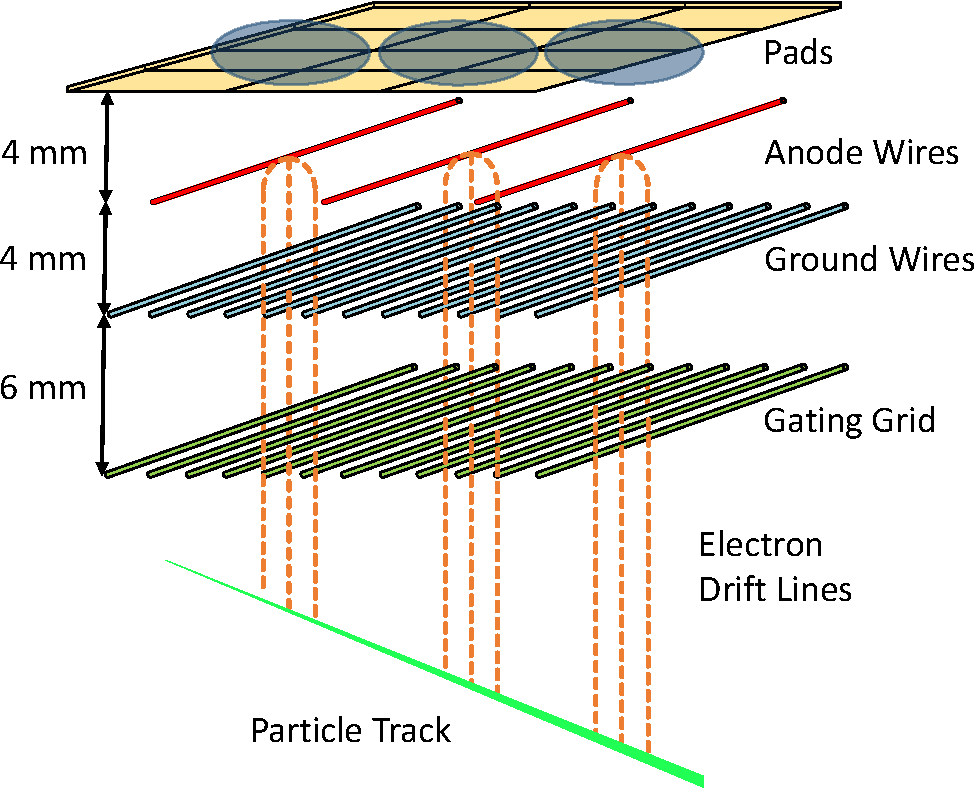
\includegraphics[width=.45\textwidth,valign=t]{wires_open.pdf} \label{fig:wires_open}}}%
    \qquad
    \subfloat[Wires closed]{{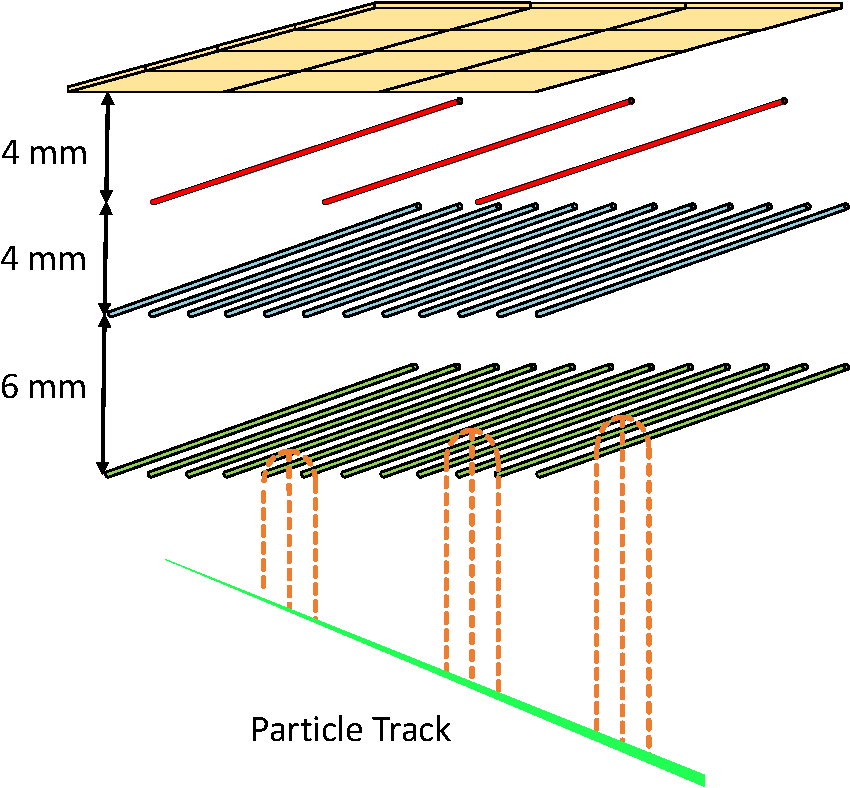
\includegraphics[width=.39\textwidth,valign=t]{wires_closed.pdf} \label{fig:wires_closed}}}%
    \caption{Cartoon depiction of electron drift lines going through the various wire planes.}%
    \label{fig:wires}%
\end{figure}

\begin{figure}[!htb]
\centering
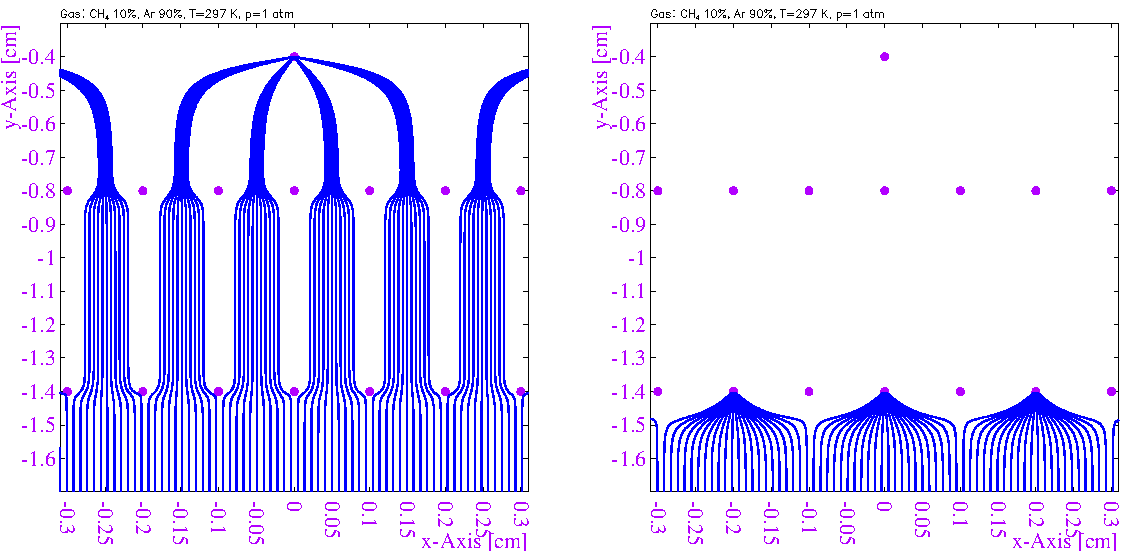
\includegraphics[width=\textwidth]{gg_onoff.pdf}
\caption{Garfield simulations of the on and off configuration of the gating grid with the drift lines of electrons through all of the grids.}
\label{fig:gg_onoff}
\end{figure}


Both configurations of the gating grid were measured and simulated. To measure the electron transparency in the on configuration all wires were set to the same voltage $V_{avg}$, and the anode wires were lowered to \SI{500}{\volt}. By lowering the voltage of the anode wires we could measure the large charge of the beam without saturating the electronics. The average charge deposited in the chamber was measured as a function of $V_{avg}$. Changing the average voltage required a different top perimeter resistor value according to Eq.~\ref{eq:TP_resistor}. Several runs were taken ranging from \SIrange{-198}{-40}{\volt}, with and without the magnetic field. Theoretically the most negative value represents 100\% electron transparency and was used as the reference run in which we scaled all measurements to. The measured electron transparency, $T$, was estimated as $T_i = \langle dE/dx\rangle_i /{\langle dE/dx\rangle}_{ref}$, where $\langle dE/dx\rangle_{ref}$ represents the average energy loss of the reference run, and $\langle dE/dx\rangle_i$ is the average energy loss for the $i^{th}$ run. Figure~\ref{fig:ggAvgTrans} shows the measured transparency as a function of $V_{avg}$, as compared with the corresponding Garfield simulation \cite{garfield++}. The average gating grid voltage used in the experiment was \SI{-171}{\volt} to ensure we were well within the 100\% transparency region. 

To measure the electron transparency as a function of the difference voltage $\Delta V$, the average voltage was first set to 100\% transparency, $V_{avg}=\SI{-171}{\volt}$, and the difference voltage was added and subtracted from alternating wires. Figure~\ref{fig:ggDeltaVTrans} shows the result of the simulation and experiment with and without the magnetic field. By introducing the magnetic field the required voltage to close the grid increased as expected. In the experiment we selected the value of $\Delta V = \SI{65}{\volt}$ to ensure we were well within the region of 0\% transparency. In both the on and off configurations good agreement was seen with the corresponding Garfield++ simulations when accounting for statistical error in the MC simulations and in the data.   



\begin{figure}[!htb]%
    \centering
    \subfloat[On configurations where all wires are the same voltage.]{{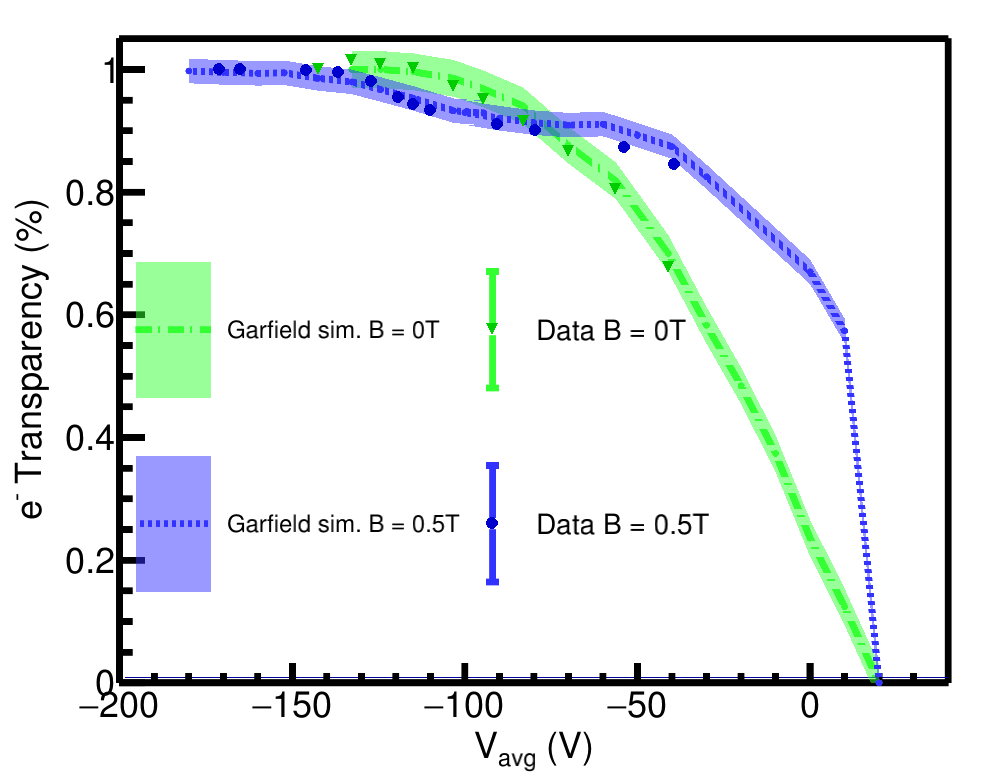
\includegraphics[width=.45\textwidth,valign=t]{averageTransparency.png} \label{fig:ggAvgTrans}}}%
    \qquad
    \subfloat[Off configuration where adjacent wires have a voltage difference of $2 \Delta V$.]{{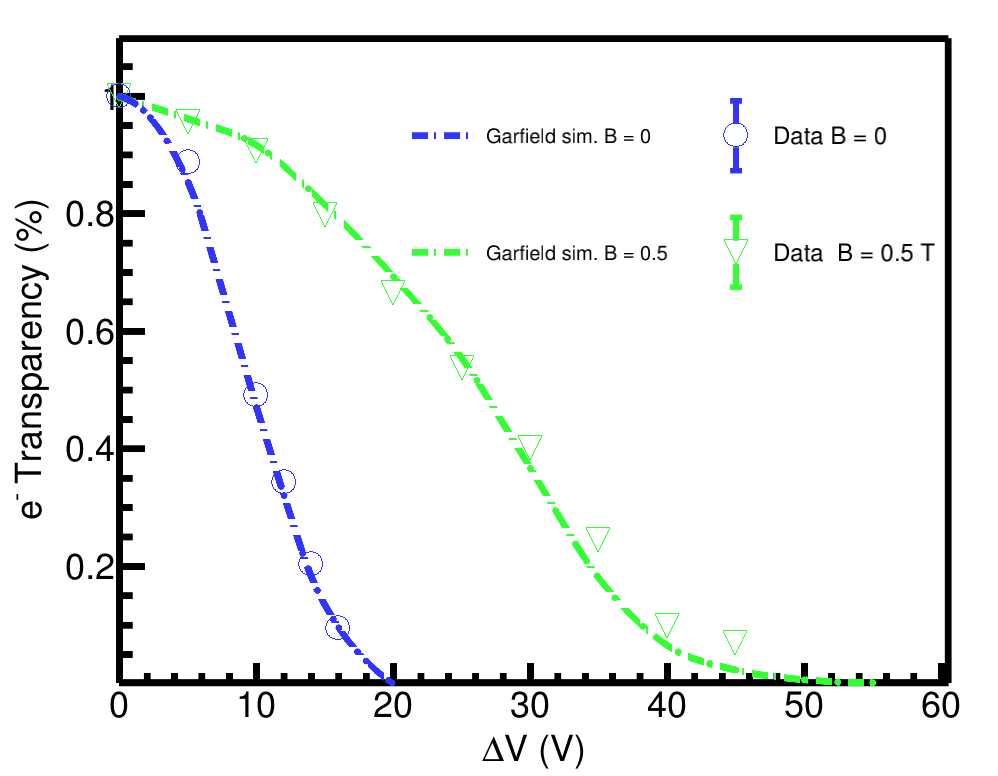
\includegraphics[width=.45\textwidth,valign=t]{transparencyDeltaV.png} \label{fig:ggDeltaVTrans}}}%
\caption{Electron transparency as measured and simulated in the on and off configurations of the gating grid.}    
\label{fig:ggTrans}
\end{figure}


The anode wires are made of very thin Gold plated Tungsten wires, about \SI{20}{\micro\metre} in diameter. They are biased to high voltages of about  \SI{e3}{\volt} which creates a very high electric field very close to the anode wire. As the electron approaches the anode wire, the field gets strong enough that the kinetic energy gained between collisions exceeds the ionization potential of the gas knocking out more electron-ion pairs in the gas. This happens over succesive  collisions creating an avalanche effect amplifying the electron current.  The final number of electrons produced depends on the anode wire voltage and the gas properties. The absolute gas gain was not experimentally determined but it was calculated in a Garfield simulation. For the experimental data pertaining to this disertation, the anode wires were biased to two different voltages. We will refer to the voltage \SI{1460}{\volt} as the \emph{high voltage} and \SI{1214}{\volt} as the \emph{low voltage}. Two sections of the anode wire plane, were biased with the lower voltage setting to minimize the effects of a leakage of secondary electrons around the end of the gating grid \cite{jon}.


 Figure~\ref{fig:anodegain} shows the electron distribution for the total number of electrons produced in a avalanche process created by a single electron. The distribution follows the expected Polya distribution, and the MC data in the simulation was fitted with a Polya function \cite{blumrol}, which can be expressed as,

\begin{equation}
P(x) = A_0^{-1}\cdot \frac{A_1^{A_1}}{\Gamma(A_1)} \left(\frac{x}{A_0}\right)^{A_1-1}e^{\frac{-A_1x}{A_0}}.
\end{equation}

For the voltage of \SI{1460}{\volt} the parameters of the fit are $A_0=903.9$ and $A_1=1.50$ and for the voltage of \SI{1214}{\volt} the parameters are $A_0=150.0$ and $A_1=1.47$. These Polya distribution fits will be important later as the input to the Monte Carlo simulations of the detector response in Section~\ref{sec:monteCarlo}.



\begin{figure}[!htb]
\centering
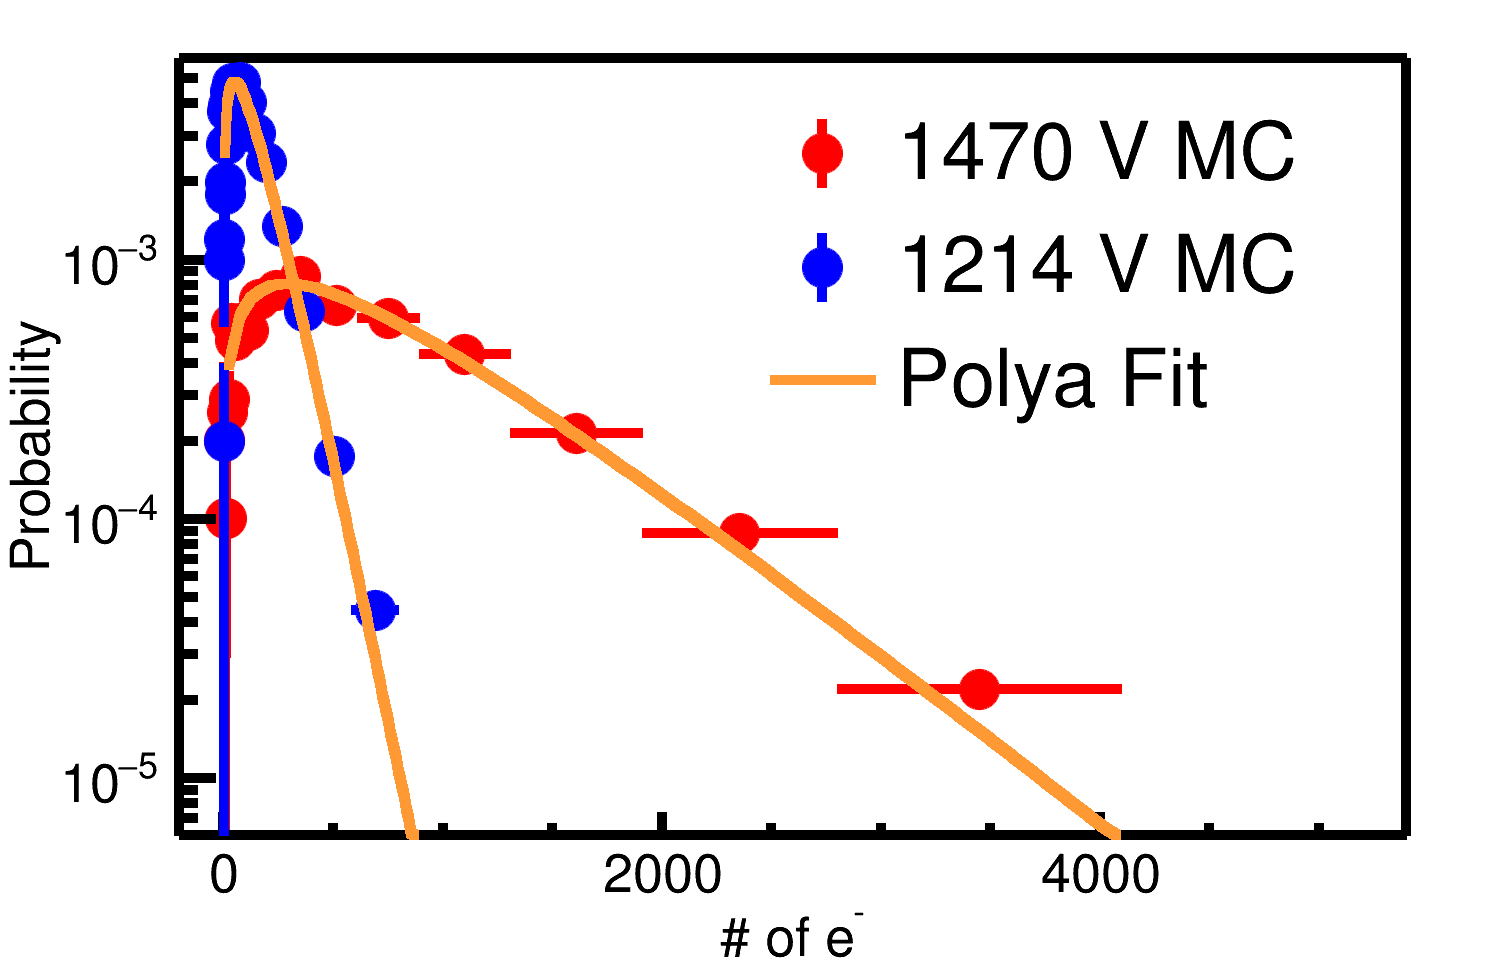
\includegraphics[width=.8\textwidth]{gain.png}
\caption{Number of electrons produced in a single avalanche on an anode wire. Two different voltages were simulated using Garfield++ at 1470 $V$ and 1214 $V$. The expected Polya distribution fit is also given in yellow.}
\label{fig:anodegain}
\end{figure}



Care must be taken to choose the resister ($R_{TP2}$) that connects the field cage divider chain to the top plate. The end of the field cage nearest to the top plate is at the same potential as the Aluminum top perimeter piece to which the field cage is glued. This top perimeter piece forms a horizontal surface that is an equipotential representing the last ring. The voltage difference between the average voltage on  the gating grid and the voltage of the top perimeter influences the electric field just below the gating grid. If $R_{TP2}$ is incorrectly chosen, the electric field near the gating grid will be different for electrons that pass near the field cage walls than it is for electrons in the center of the TPC,  causing distortions of the tracks in the TPC. This requires the value for $R_{TP2}$ to be chosen correctly. 

To understand how to calculate $R_{TP2}$ we imagine the space between the cathode and the gating grid can be split into two virtual volumes, Region 1 defined as the space between the cathode and the top-perimeter, and Region 2 defined between the top-perimeter and the gating-grid. The magnitude of the electric field in the region between the top-perimeter and the cathode, $E_1$, is defined as,

\begin{equation}
E_1 = \frac{V_{g.g.} - V_{tp}}{ y_{g.g.} - y_{tp} },
\end{equation}
where  $V_{g.g.}$, $V_{tp}$ , $y_{g.g.}$, and $y_{tp}$ are the voltages and vertical y-positions of the gating-grid and top-perimeter respectively. The y-position here refers to the center of the electrodes. The magnitude of the electric field in the region between the top-perimeter and the cathode, $E_2$, is defined as,

\begin{equation}
E_2 = \frac{V_{tp} - V_{cath}}{ y_{tp} - y_{cath} },
\end{equation}
where  $V_{tp}$, $V_{cath}$ , $y_{tp}$, and $y_{cath}$ are the voltage and vertical y-position of the top-perimeter and cathode respectively. The y-position of the cathode is defined as the face of the cathode. The condition for a smooth electric field across these two virtual volumes is defined as the solution to the equation $E_1 = E_2$. Substituting Eq.~\ref{eq:FCstrip} for $V_{tp}$ -- $n=50$ -- we can solve for the effective resistance of the top perimeter $R_p$ as, 

\begin{equation}
R_p = 49 \cdot R  \left(\frac{ y_{g.g.} - y_{cath} }{ y_{TP} - y_{cath} \frac{V_{cath} - V_{gg}}{V_{cath}} }- 1 \right),
\label{eq:TP_resistor}
\end{equation}

where the relevant vertical dimensions are $y_{g.g.} - y_{cath} = \SI{497.3}{\milli\metre}$ and $y_{tp} - y_{cath} = \SI{490}{\milli\metre}$. The value of $R_{TP2}$ can then be calculated from Eq.~\ref{eq:Reff}.


\subsection{Pad Plane}
The pad-plane is a multi-layer circuit board which is segmented into \SI{11.5}{\milli\metre} x \SI{7.5}{\milli\metre} charge sensitive pads, arranged in an array of 108 x 112 pads in the x and z-directions respectively; making 12096 pads in total. There is an insulating gap of \SI{0.5}{\milli\metre} on each side separating the pads so that the effective area covered by the pads is \SI{1344}{\milli\metre} x \SI{864}{\milli\metre}. There is a via and trace coming from each pad, through the board, to the opposite side of the pad plane, and is arranged in a surface pads which is readout by a surface mount SAMTEC connector. Figure~\ref{fig:padplane} shows the pad plane boards being glued to the top plate and the holes which allow for the readout of pads. The pads were gold plated for excellent electric conduction properties. 

\begin{figure}[!htb]
\centering
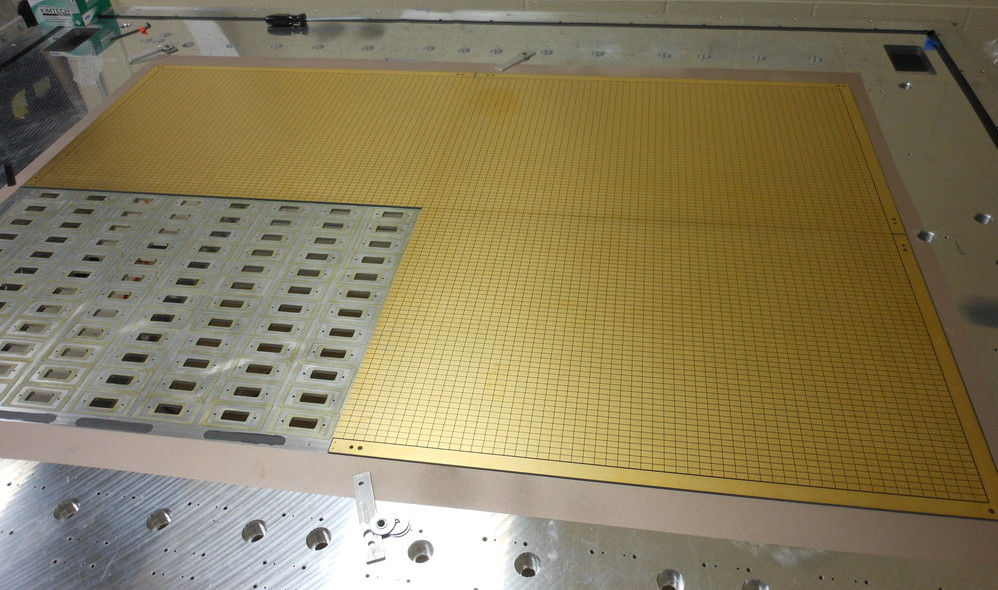
\includegraphics[width=.8\textwidth]{3boards_ps.jpg}
\caption{Figure of the pad plane boards being glued to the top plate. }
\label{fig:padplane}
\end{figure}


\subsection{Electronics}

Signals in the S$\pi$RIT TPC are amplified and digitized by the recently developed Generic Electronics for TPCs (GET) \cite{get}.  Short cables transmit the signals from the surface mount connectors, through a circuit protection board called ZAP, to the inputs of the AGET chips which are mounted to the AsAd board as seen in Figure~\ref{fig:getzap}. Each AGET chip services 64 pads (63 pads are connected in our case). Four AGET chips are mounted on one AsAd  motherboard. Figure~\ref{fig:aget} is the schematic of each  AGET chip which contains a charge sensitive pre-amplifier, several other stages of amplifiers, and a Switched Capacitor Array (SCA) with a maximum of 512 time buckets which operates in a circular readout buffer. The sampling frequency can be adjusted from 1 to \SI{100}{\mega\hertz}. The gain of each AGET can be configured as 0.12, 0.24, 1.0, or \SI{10}{\pico\coulomb} over the whole dynamic range, and the analog-to-digital converters (ADCs) on each AsAd board provides 12 bit resolution. The peaking times of the shaping amplifiers can be set to 69, 117, 232, 501, 720, or \SI{1014}{\nano\second}. In this experiment, the gain was set to the highest setting, 0.12 \si{\pico\coulomb}, the peaking time \SI{117}{\nano\second}, and the sampling frequency \SI{25}{\mega\hertz} (resulting in \SI{40}{\nano\second} time buckets). 

\begin{table*}[!htb]
\centering
\ra{1.3}
\begin{tabular}{@{}rr@{}}\toprule 
\multicolumn{2}{c}{GET electronics settings}\\
\midrule
ADC bit range       & 14 bits \\
Sampling frequency  & 1-100 MHz \\
Dynamic range       & .12, .24, 1.0, 10pC \\
Peaking time        & 69,117,232,501,720,1014 ns \\
Time bucket range   & 512\\
\bottomrule
\end{tabular}
\caption{Summary of range of GET electronics settings. }
\label{tb:getoverview}
\end{table*}

\begin{figure}[!htb]
\centering
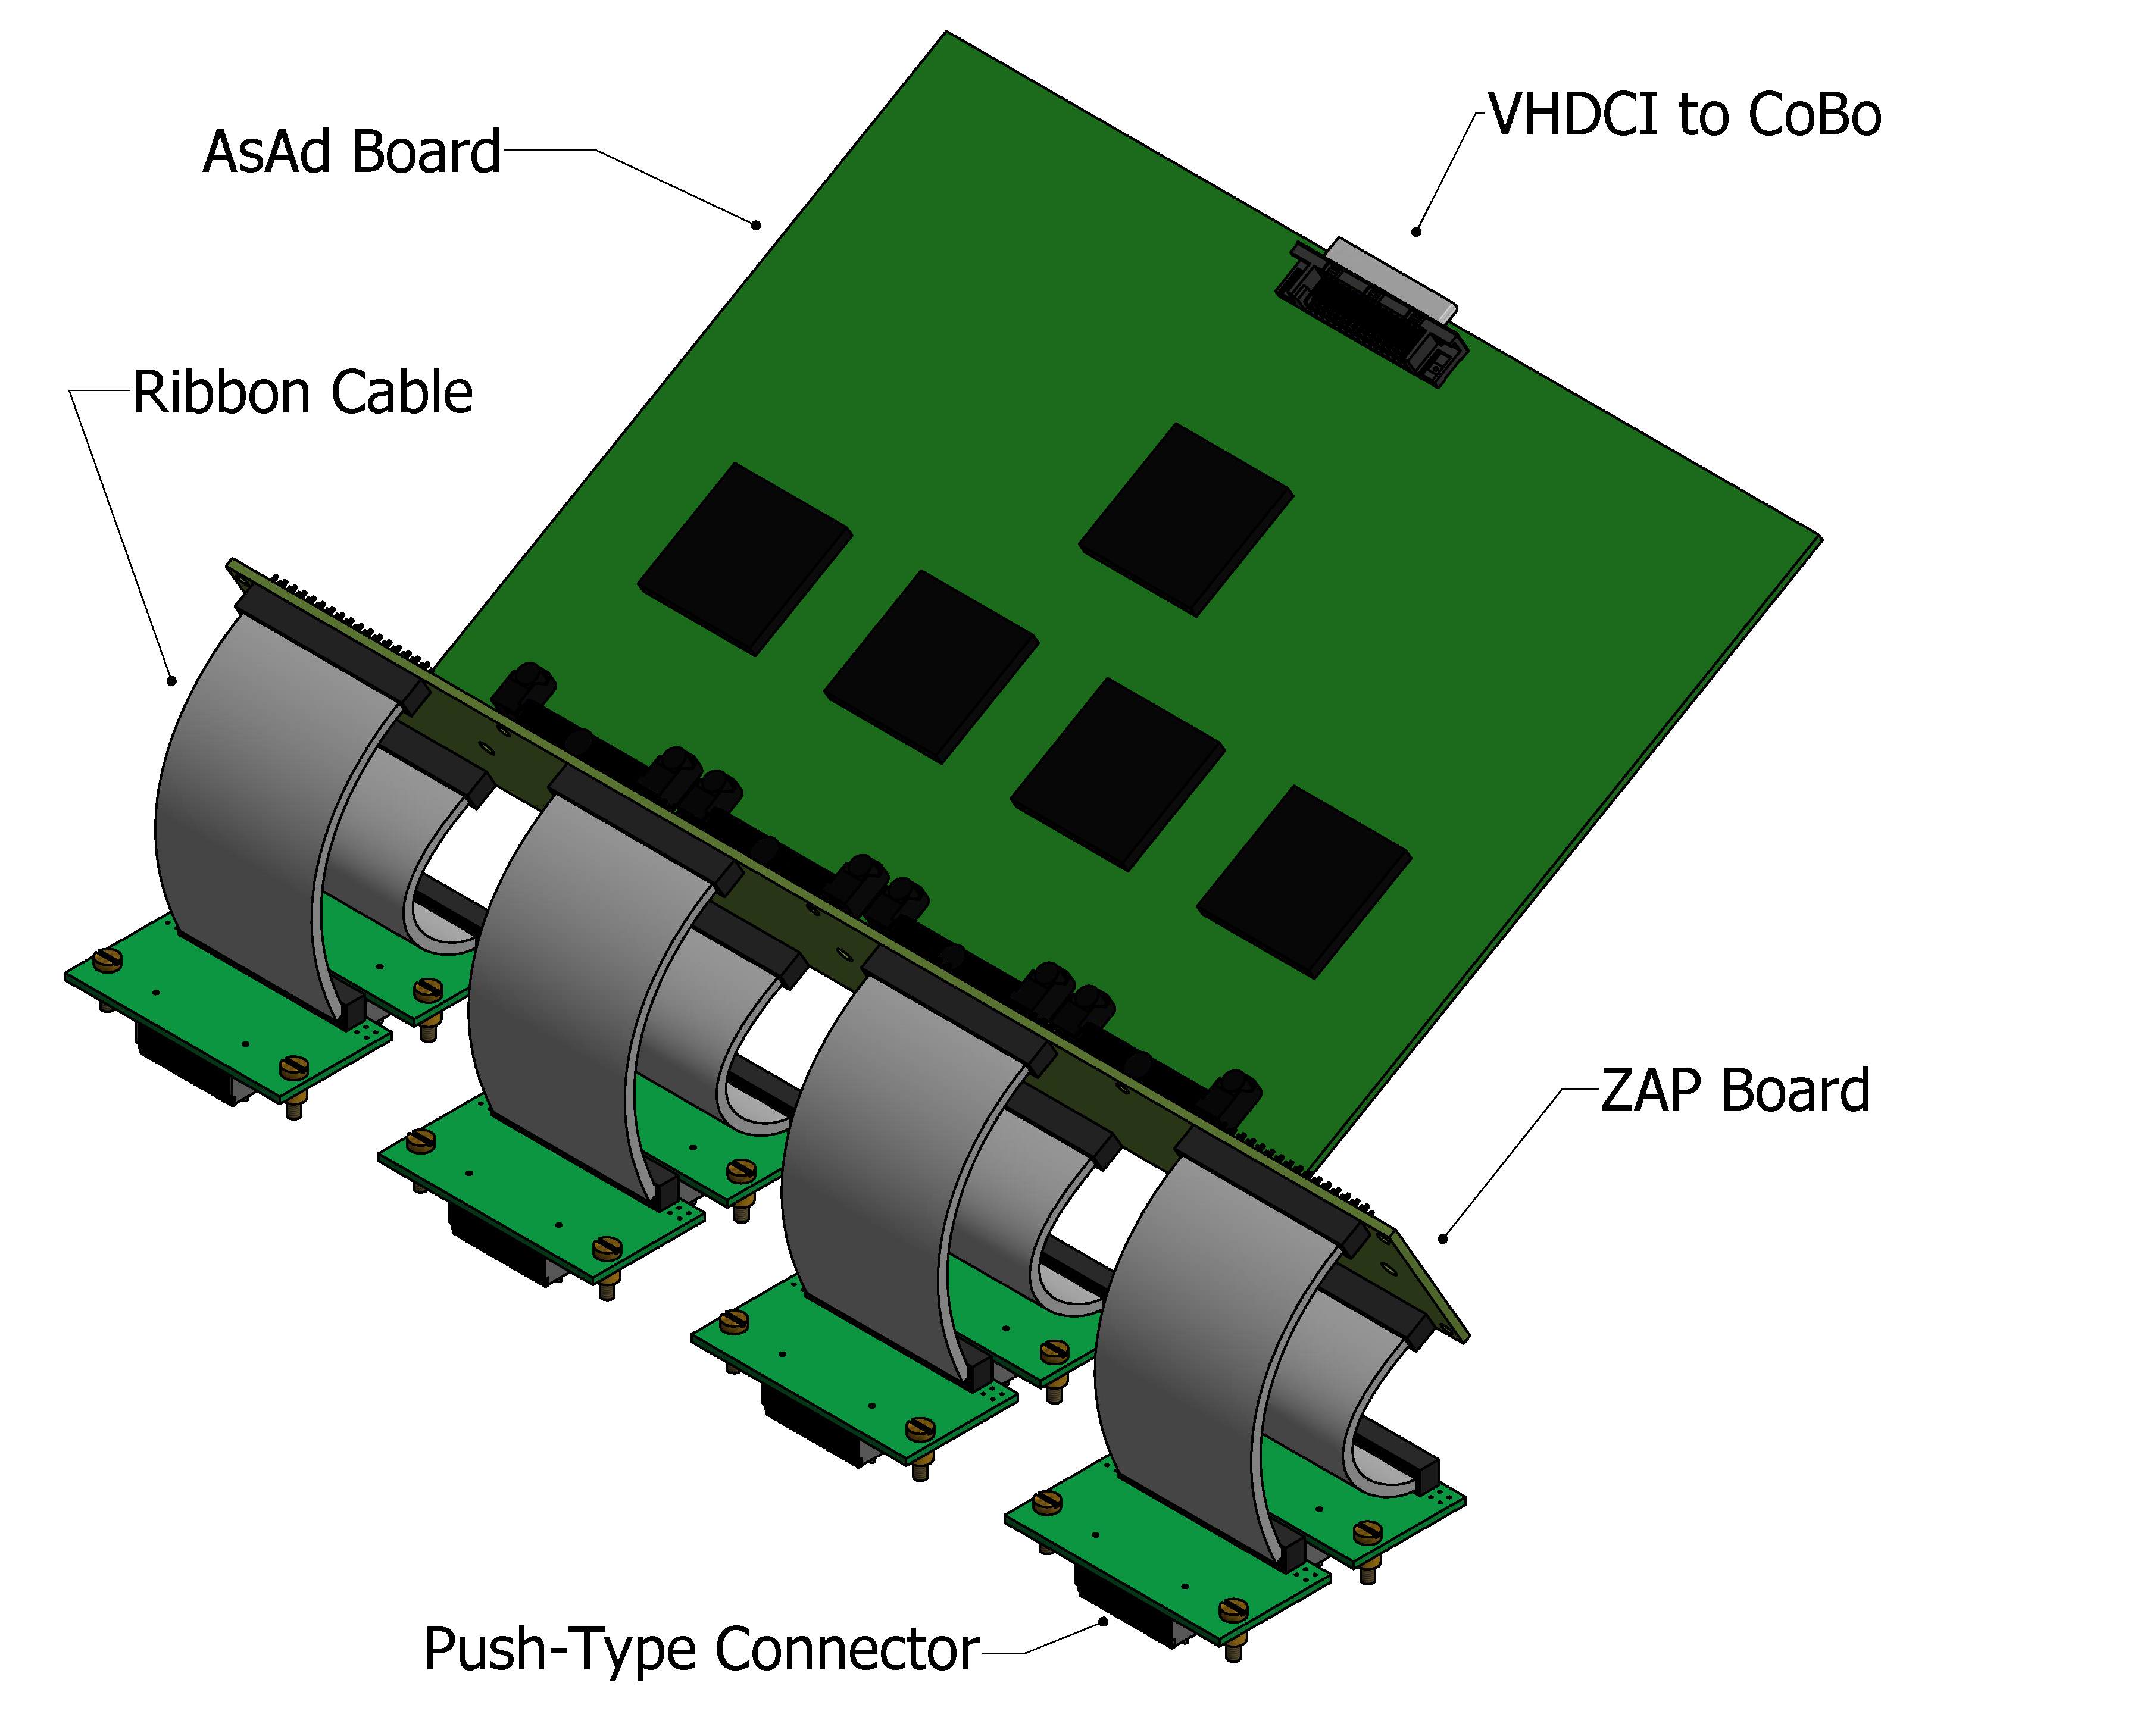
\includegraphics[width=.5\textwidth]{GET_and_ZAP.pdf}
\caption{Drawing of the ZAP and AsAd board which is connected to the surface pads on the backside of the pad-plane.}
\label{fig:getzap}
\end{figure}



\begin{figure}[!htb]
\centering
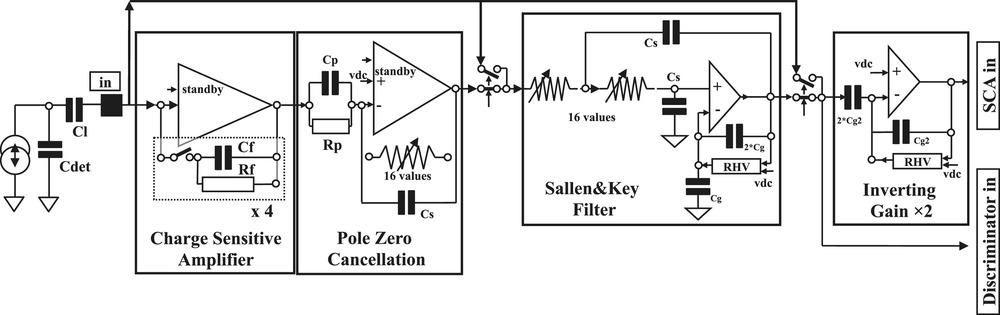
\includegraphics[width=\textwidth]{AGETfncn.jpg}
\caption{Schematic of the internals of the AGET chip from \cite{get2}}
\label{fig:aget}
\end{figure}


\begin{figure}[!htb]
\centering
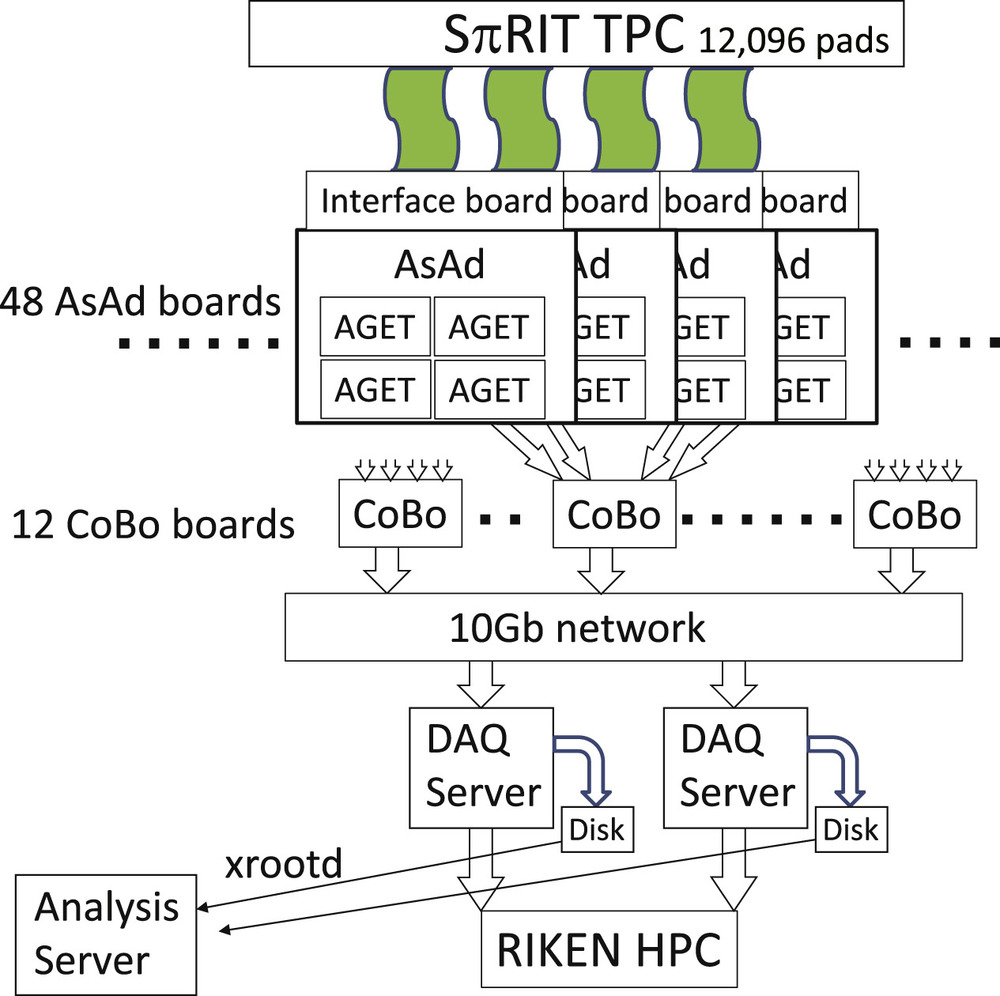
\includegraphics[width=.5\textwidth]{GETlayout.jpg}
\caption{Readout structure of the AsAd boards and CoBo board structures. Also the relevant components of the DAQ system.}
\label{fig:coboDAQ}
\end{figure}

After each AsAd board has digitized the data it is sent to the Concentration Boards (CoBo). Each CoBo board can concentrate the data from 4 AsAd boards. The Multiplicity, Trigger, and Time module (MuTanT) \cite{get} provides the common trigger signal for all CoBo boards.  Each board sends the data to the DAQ server which writes to disk the data from each board, which was handled by two separete DAQ servers; saving to one common analysis server. The data could then be analyzed using the RIKEN High Performance Computing (HPC) cluster or moved to the NSCL or MSU cluster for analysis. The Aget 2.0, asad 2.1, and cobo 1.0 firmware versions were used in this analysis. 

\section{Energy loss in material}
\label{sec:energyloss}

The average energy loss in a material can be described by the Bethe-Bloch equation,
\begin{equation}\label{eq:bb}
\frac{dE}{dx} = \frac{4\pi NZ^2e^4}{mc^2\beta^2} (\ln \frac{2mc^2\beta^2\gamma^2}{I} - \beta^2),
\end{equation}
where $N$ is the number density of electrons in the medium, $e$, the elementary charge, $mc^2$, is the rest mass of the electron, $Z$ is the charge of the traversing particle, $I$ is the mean excitation energy of the medium, and $\beta$ is the velocity of the particle \cite{blumrol}. Yet there is a large variation in energy loss around this mean value. The statistical variation of energy loss in a material was described by Landau \cite{landau} and later better described by Shulek \cite{shulek} and Bichsel \cite{bichsel1}. In both approximations it is described by a most probable energy loss value, with a long, high-energy loss tail. The solid curve in Figure~\ref{fig:straggling} shows the energy loss distribution in Ar gas for a proton with momentum \SI{3.4}{\giga\eVperc} \cite{bichsel}. The dashed line is the distribution under the Landau assumptions. The mean energy loss $\langle\Delta\rangle$ is significantly shifted from the most probable value $\Delta_p$, due to the long high energy tail.  Because of this long tail, for a finite set of energy loss measurements along a given track, the mean value is very unreliable. The most probable energy loss is the better observable which can be obtained either through fitting of the observed distribution or through the truncated mean method. 

\begin{figure}
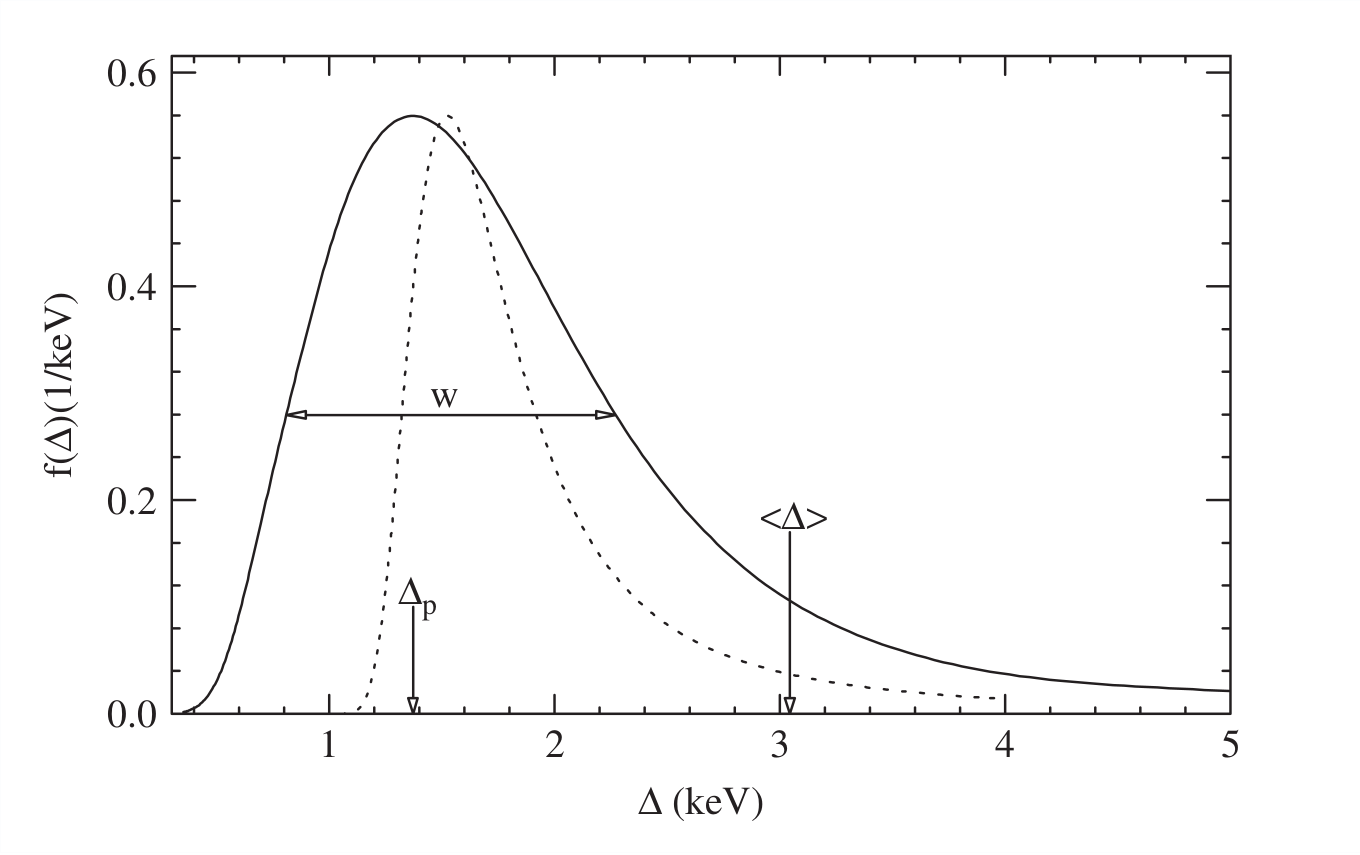
\includegraphics[width=\textwidth]{bichsel.png}
\caption{Energy loss distribution of a $\beta\gamma$ = 3.6 particle in Ar gas taken from \cite{bichsel}}
\label{fig:straggling}
\end{figure}

The truncated mean is the average mean value calculated after throwing away the top fraction of the highest energy loss entries. This approximates the most probable value without performing a fit to a known distribution. If a set of $n$ observed energy loss values, $\Delta_i/x$, in a given track are sorted from smallest to largest value. The truncated mean $C$, is calculated from the reduced set of points $n_t = f_r n$ as,

\begin{equation}
C = \frac{1}{n} \sum\limits_{i}^{n_t} \Delta_i/x,
\label{eq:truncmean}
\end{equation}

where $f_r$ is the cut off fraction. In this Dissertation, a value of 0.7 was used. This was the same value used in the STAR TPC collaboration \cite{starsyst}. 




%Suppose $E$ represents the set of $N$ energy loss points measured, sorted from lowest to highest energy loss. The $j^{th}$ index marks the position where  $i > j$ entries represent the highest value of energy loss measurements, where their fraction of the total set is expressed as, $f_c = \sum_{i>j} E_i/ \sum_i E_i$. The truncated mean is expressed as the mean value of the remaining energy loss measurements, throwing away the top $f_c$ fraction, expressed as,

%\begin{equation}
%\langledE/dx\rangle_t = \frac{\sum_{i < j} E_i}{N}
%\label{eq:truncatedM}
%\end{equation}

 %A full description of the energy loss distribution can be described in CITE HERE.


\subsection{Gas Properties}
The gas used was a mixture of 90\% Ar and 10\% Methane ($\mathrm{CH_4}$) by volume (P10 gas), and operated just under atmospheric pressure 1 atm. The gas was continually flowed through the field cage and exited into the enclosure volume, finally passing through a bubbler to atmosphere. The gas purity was monitored with an oxygen and water monitor which are the two most concerning contaminants. The water never exceed  50 ppm  and the oxygen level never exceeded 50 ppm, which are the two main contaminants in the gas which can absorb primary electrons \cite{tpcAging}. Figure~\ref{fig:driftvel} shows the drift velocity of P10 gas at 1 atm (\SI{760}{\torr}) as a function of the reduced electric field value given in units of \si{\volt\per\centi\metre\per\torr}. Operating near the peak value of the drift velocity curve minimized the change in the drift velocity as the effective field slightly changes due to slight variations in the pressure. The electric field in the experiment was \SI{125}{\volt\per\centi\per\metre} at \SI{760}{\torr}, giving a reduced electric field \SI{0.17}{\volt\per\centi\metre\per\torr}.

\begin{figure}[H]
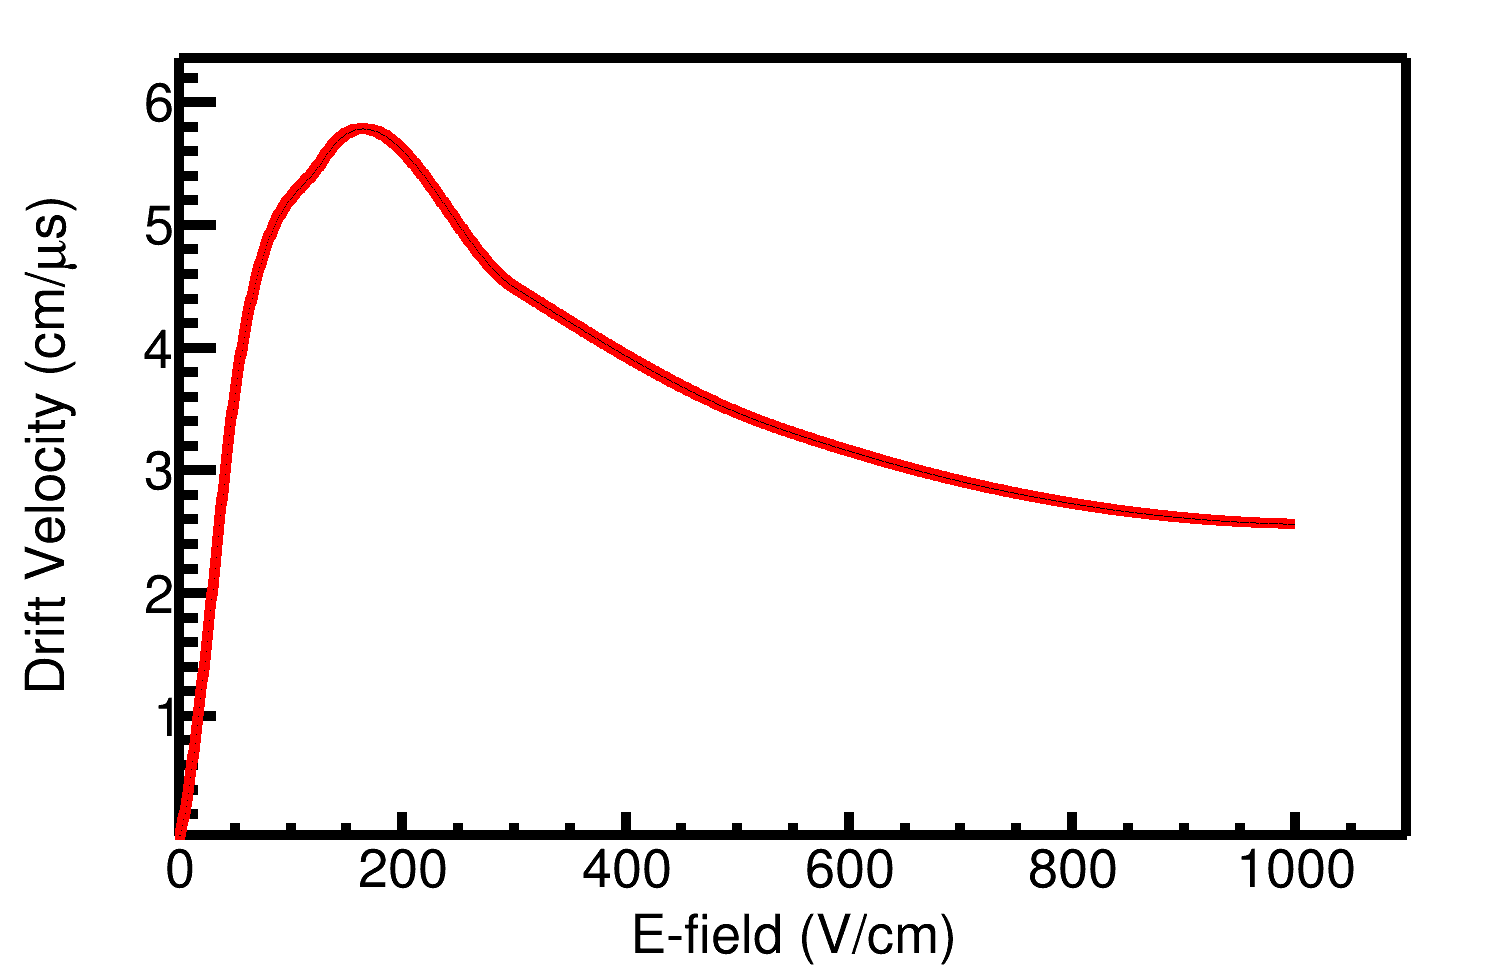
\includegraphics[width=\linewidth]{driftvel.png}
\caption{Drift velocity of electrons in P10 gas as a function of the reduced electric field.}
\label{fig:driftvel}
\end{figure}

The general formula for the drift velocity, $d\vec{x}/dt$, of an electron in the presence of electric and magnetic fields, $\vec{E}$ and $\vec{B}$, can be expressed in the Langevin equation as,  

\begin{equation}
\frac{d\vec{x}}{dt} = \frac{\mu}{1+(\omega\tau)^2}\Big(\vec{E} + \omega\tau\frac{\vec{E}\times\vec{B}}{|\vec{B}|}+\omega^2\tau^2\frac{\vec{E}\cdot\vec{B}}{|\vec{B}|^2}\vec{B}\Big),
\label{eq:elecdrift}
\end{equation}

where $\mu=\SI{5.43}{\centi\metre\per\second}$ is the signed drift velocity, $\omega=\SI{8.79e10}{\radian\per\sec}$ is the cyclotron frequency, and $\tau=\SI{2.48e-11}{\second}$ is the collision parameter for a particular gas \cite{blumrol}.

Several properties of the gas were simulated in Garfield including the longitudinal and transverse diffusion, $\sigma_l$ and $\sigma_t$ respectively, and the electron and ion drift velocities, $v_d$ and $v_i$ respectively for the experimental electric field of \SI{125}{\volt\per\centi\metre}. The results are summarized in Table~\ref{tb:gasprop}.


\begin{table}[!htp] % not just 'h!'
\centering % not a center environment
\begin{tabular}{
  @{}
  l
  S[table-format=1.2]
  S[table-format=1.2]
  S[table-format=1.2]
  S[table-format=1.2]
  S[table-format=5.2]
  S[table-format=5.2]
  @{}
}
\toprule
Gas properties &
 {$\sigma_{t}$} &
 {$\sigma_{l}$} &
 {$v_{d}$} &
 {$v_{i}$}  &
 {$G_{h}$} &
 {$G_{l}$} \\
&
  {($\si{\centi\meter}^{-1/2}$)} &
  {($\si{\centi\meter}^{-1/2}$)} &
  {(\si{\centi\meter\per\micro\second})} &
 {(\si{\centi\meter\per\micro\second})} \\

\midrule
\phantom{abc}   &.024   &.034  &5.43  &  \num{2.05e-4} &  903   &150     \\
\bottomrule
\end{tabular}

\caption{Gas properties of P-10 gas at 1 atm pressure.}
\label{tb:gasprop}
\end{table}

%Add table for gas diffusion 

\section{Pad Response Function}
\label{sec:prf}
Each electron avalanche produces a two-dimensional image charge on the pad plane, as shown in the cartoon in Figure~\ref{fig:2DPRF}, where the projection of the charge distribution onto the $x$ and $z$ axis of this distribution are labeled as $\rho(x)$ and $\rho(z)$ respectively. If $\rho(x,z)$ represents the charge distribution on the pad-plane, the total charge observed a particular pad, $Q$, is expressed as,

\begin{equation}
Q(x_o,z_o) = \int_{z_o - \frac{l}{2}}^{z_o + \frac{l}{2}} \int_{x_o - \frac{w}{2}}^{x_o + \frac{w}{2}} \rho(x-x_o\textprime,z - z_o\textprime) dxdz,
\label{eq:prfpadCharge}
\end{equation}

where $x_o$ and $z_o$ represent coordinates of the center of that pad, $x_0\textprime$ and $z_o\textprime$ are the coordinates of the avalanche, $w$ is the width, and $l$ is the length of the pad. The total charge observed for a given track is a superposition of all avalanches on all the anode wires. Typically in a TPC, the charges on each pad are grouped into clusters, and it is practical to cluster in only one direction. Therefore we will speak about the marginal probability distribution over a given layer of pads (x-distribution), or row of pads (z-distribution). The marginal distribution for a given layer can be written as,
\begin{equation}
\rho_x(x) = \int_{z_o - \frac{l}{2}}^{z_o + \frac{l}{2}} \rho(x,z)dz,
\end{equation}

and over a given row can be written as,

\begin{equation}
\rho_z(z) = \int_{x_o - \frac{w}{2}}^{x_o + \frac{w}{2}} \rho(x,z)dx.
\end{equation}

By substituting the variables  $\lambda_x = x - x_o\textprime$, and $\lambda_z = z - z_o\textprime$, we can express the charge distribution independent of the avalanche location. The Pad Response Function (PRF) along the x-direction of a given layer can be written as,

\begin{equation}
P_X(\lambda_{x_o}) = \frac{ \int_{\lambda_{x_o}-\frac{w}{2}}^{\lambda_{x_o} + \frac{w}{2}} \rho_x(\lambda_x)d\lambda_x } {\int_{-\infty}^\infty \rho_x(\lambda_x)d\lambda_x     },
\label{eq:prflayer}
\end{equation}

where $\lambda_{x_o} = x_o - x_o\textprime$; in a similar manner for the situation we cluster along the z-direction  of a given row the PRF can be written as,

\begin{equation}
P_Z(\lambda_{z_o}) = \frac{ \int_{\lambda_{z_o}-\frac{l}{2}}^{\lambda_{z_o} + \frac{l}{2}} \rho_z(\lambda_z)d\lambda_z }{\int_{-\infty}^\infty \rho_z(\lambda_z)d\lambda_z  },
\label{eq:prfrow}
\end{equation}

where $\lambda_{z_o} = z_o - z_o\textprime$.


\begin{figure}[!htb]
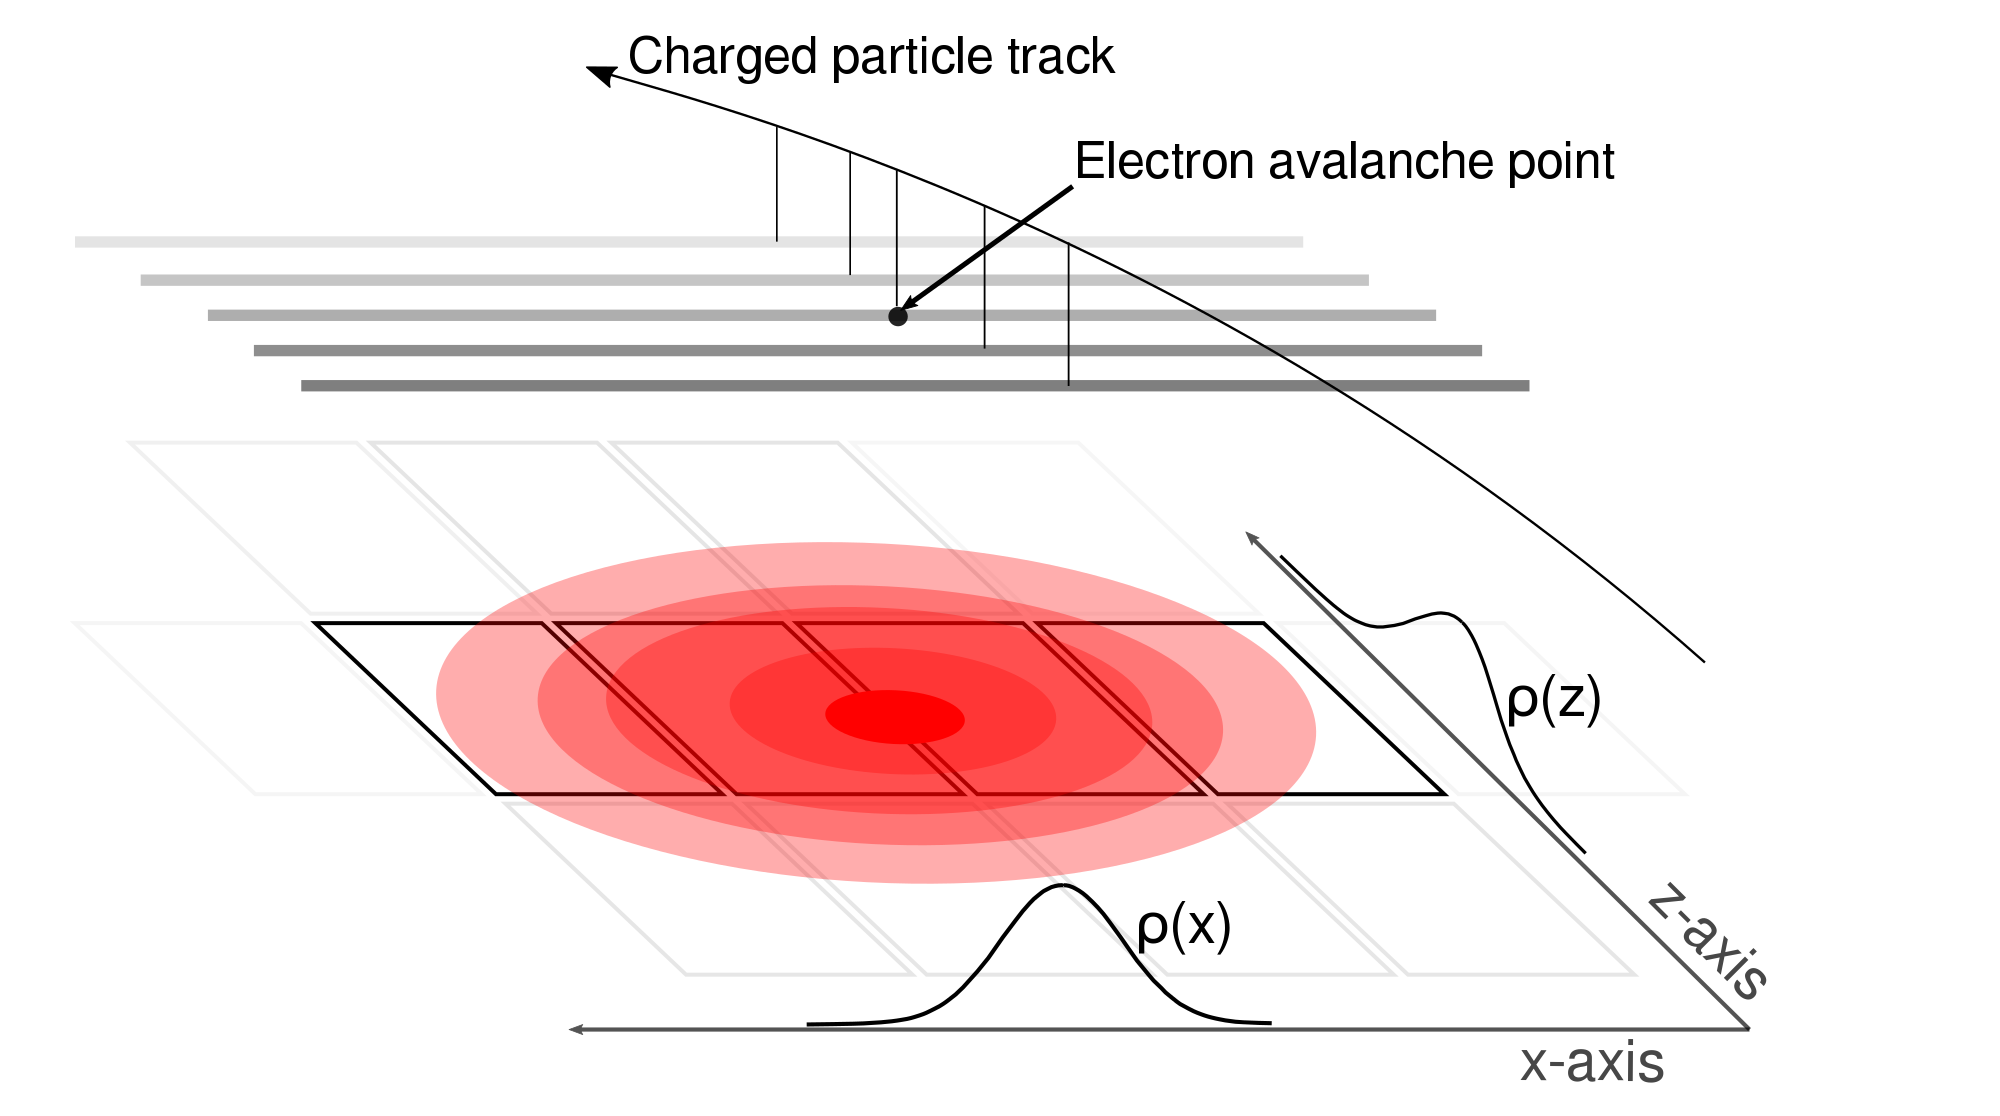
\includegraphics[width=\linewidth]{padsat_Large}
\caption{A cartoon illustration of the charge distribution resulting from an electron avalanche on one wire and the projections of the distribution onto the two axis $\rho(x)$ onto the x-axis and $\rho(z)$ onto the z-axis. The orientation of the wire planes is flipped upside down to display the perspective better.}
\label{fig:2DPRF}
\end{figure}

Gatti \cite{gatti} derived a semi-empirical formula for the charge distribution in a simple multi-wire TPC given as, 
\begin{equation}\label{eq:gatti}
\begin{split}
PRF_{\mathrm{Gatti}}(\lambda)
& = \frac{K_{1}}{K_{2}\sqrt{K_{3}}}\bigl[\arctan(\sqrt{K_{3}}\tanh\bigl[K_{2}\bigl(\frac{\lambda}{h}+\frac{w}{2h}\bigr)\bigr]) \\
& - \arctan(\sqrt{K_{3}}\tanh\bigl[K_{2}\bigl(\frac{\lambda}{h}-\frac{w}{2h}\bigr)\bigr])\bigr] \\
\end{split}
\end{equation}

where $w$ is the width of the pad, $h$ is the distance of the anode plane to the pad plane, and $\lambda$ is the distance of the pad center to the avalanche point. It is a single parameter equation where the two parameters $K_1 = \frac{K_{2}\sqrt{K_3}}{4 \arctan(\sqrt{K_3})}$ and $K_2 = \frac{\pi}{2}\left(1-\frac{\sqrt{K_{3}}}{2}\right)$ depend on the parameter $K_3$, which is a function of the ratio of the anode wire diameter to the distance of the anode wires to the pad plane. $K_3$ can be looked up in a graph in \cite{blumrol} and \cite{gatti}.


\begin{figure}[!htb]
\begin{overpic}[width=\linewidth]{fig5.pdf}
\put(61,55){\contour{white}{ PRF${}_{\mathrm{Gaus}}(\lambda)$ eq. \ref{eq:gaus}  }}
\put(61,49){\contour{white}{ PRF${}_{\mathrm{Gatti}}(\lambda)$ eq. \ref{eq:gatti} }}
\end{overpic}
\caption{Experimental pad response function of many events for a crossing angle of $85^{\circ} < \theta \leq 90^{\circ}$.  }
\label{fig:expprf}
\end{figure}


Since we take the marginal distributions only along one layer or row of pads, correlations are introduced in the PRF from adjacent layers or rows which cause slight deviations from the expected Gatti distribution. Also, analytic PRFs only exist for classical multi-wire TPCs. For these reasons it is useful to experimentally measure the PRF and fit it with an empirical function, typically a Gaussian, to describe its behavior. The method for extracting the experimental PRF will be discussed latter, but by averaging over many events in the experimental data, the resulting PRF for the S$\pi$RIT TPC is shown in Figure~\ref{fig:expprf}. Here we see the deviations from the expected analytic Gatti distribution (black curve), whereas fitting with a two parameter Gaussian function (red curve) gives a better description of the  data, Eq.~\ref{eq:gaus}, with the two parameters being the normalization coefficient, $N_0$, width $\sigma$, and with a mean value assumed to be 0.

\begin{equation}\label{eq:prfgaus}
PRF_{\mathrm{Gaus}}(\lambda) = N_0 e^\frac{-\lambda^2}{2\sigma^2}
\end{equation}

While the differences between the Gaussian distribution and the Gatti distribution are small for this TPC geometry, we use the Gaussian distribution because of its superior reproduction of the tails of the pad response function.   



\begin{comment}
\subsection{Considerations when constructing a TPC}
Several considerations went into the construction of the S$\pi$RI TPC which I wish to summarize and document here. All materials and glues of the TPC were selected as low out-gassing materials. Several materials (that are common place in nuclear labs), such as vacuum grease, Viton o-rings, all out-gas organic chemicals into the counter gas which damage the TPC by permanently lowering the gain over time. The organic molecules responsible are difficult to identify exactly, but lists of good and bad materials are well known in the literature from experiments. If a material we wished to used was not on these lists we placed the material in a clean chamber with the counter gas and flowed this counter gas through a small proportional counter making sure the gain did not drop at high collection rates when exposed to a high rate alpha Americium source. 

Sparking
Two volumes of gas. 
\end{comment}


\section{Radio Isotope Beam Factory (RIBF) Facility }
%Cyclotron facility overview.
%Samurai line overview.
%Beam line element overview.
%Big rips beam PID. reference 
The primary and secondary beams were produced at the Radioactive Isotope Beam Factory (RIFB) facility at RIKEN, in Wako-shi, Japan. The RIBF facility starts with two primary beam types, ${}^{132}$Xe and ${}^{238}$U, which are produced by an ion-source and accelerated to progressively higher kinetic energies by 1 linear accelerator (RILAC), and 4 different cyclotrons (RRC, fRC, IRC, and SRC), until they reach a beam energy of \SI{345}{\MeVA}. Figure~\ref{fig:samuraiBeamLine} shows the later stages of the cyclotrons and the following beam lines to which these beams can be sent. For this dissertation, the beam went through the BigRIPS spectrometer, where the specific rare isotope beams of interest were produced and on to the SAMURAI dipole where the  \spirit TPC was placed. The red box indicates the location of the experimental setup in Figure~\ref{fig:samuraiBeamLine} .


\begin{figure}[!htb]
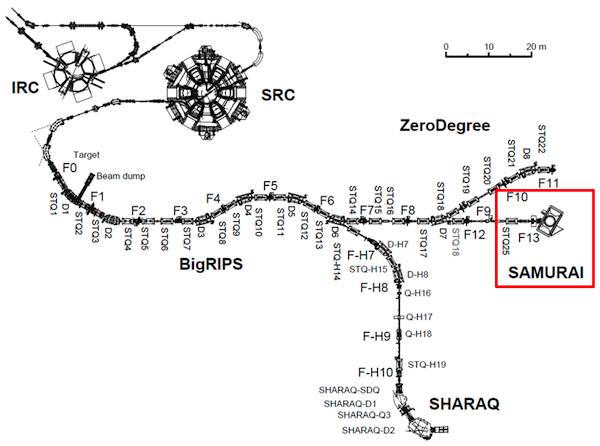
\includegraphics[width=\linewidth]{SAMURAI-beamline.png}
\caption{Overview of the RIBF, BigRIPS, and SAMURAI beamline.}
\label{fig:samuraiBeamLine}
\end{figure}

After the SCR, the primary beams impinge on a rotating \SI{3}{\milli\metre} Be target which fragments the beam into many different species. These fragments are then separated by the BigRIPS spectrometer which is tuned to the particular secondary fragment of interest. This is accomplished through several dipole magnets, slits, and wedge degraders. The resulting secondary beam is not pure and the purity depends on the capability of BigRIPS to deliver the secondary beam of choice and the primary beam used. The BigRIPS separator had many scintillators for timing, an ion chamber for Z identification and beam tracking elements used to determine the magnetic rigidity of the beam. Information from these detectors allow  allowed  identification  of the mass, charge and momentum of each isotope in the secondary beam. This information was determined beam particle by beam particle and recorded along with the TPC data on each event. With this information, it was possible to select with precision the reactions to be included in any subsequent data analysis.  

In the experimental campaign,   several beams were utilized that have  different intensities and purities. Table~\ref{tb:beams} summarizes the average qualities of the 4 secondary beams that were used in our experimental campaign. Most beams were delivered with an intensity of \SI{10}{\kilo\hertz}.

 \begin{table*}\centering
\ra{1.3}
\begin{tabular}{@{}ccccc@{}}\toprule 
 Primary Beam & Secondary Beam & Energy at mid target \si{\MeVA} & Intensity \si{\kilo\hertz} & Purity (\%) \\ [0.5ex] 
 \midrule
 ${}^{238}$U   & ${}^{132}$Sn   &  269.2  &  9.5  &  54   \\
 ${}^{238}$U   & ${}^{124}$Sn   &  270.3  &  9.1  &  10  \\
 ${}^{124}$Xe  & ${}^{112}$Sn   &  270.4  &  7.6  &  48  \\
 ${}^{124}$Xe  & ${}^{108}$Sn   &  269.3  &  7.5  &  52   \\
 \bottomrule
\end{tabular}
\caption{Primary and secondary beam properties produced in the \spirit TPC experimental campaigns. }
\label{tb:beams}
\end{table*}



\section{Experimental Setup}

The \spirit TPC was designed to fit into the dipole gap of the  dipole magnet at the end of the BigRIPS beam line. Figure~\ref{fig:experiment} shows a drawing of the \spirit TPC inside of the SAMURAI magnet chamber which was rotated to the $\ang{0}$ configuration. Typically the SAMURAI (Superconducting Analyzer for Multi-particles from Radioisotope beams) dipole magnet is operated under vacuum as a large-acceptance multi-particle spectrometer for radioactive-beam experiments. This magnet can reach magnetic fields up to \SI{3}{\tesla} at the center of the pole gap and was operated at \SI{0.5}{\tesla} for these sets of experiments. The space between the magnetic pole faces is further complicated by large bolts which protrude from the pole faces. These bolts secure the vacuum chamber to the magnet which is not practically removable; though the inside of the magnet was not operated under vacuum. This required an extensive rail system and support frame to slowly slide in the TPC over the bolts, finally raising the TPC several \si{\centi\metre} to the final height. 

\begin{figure}
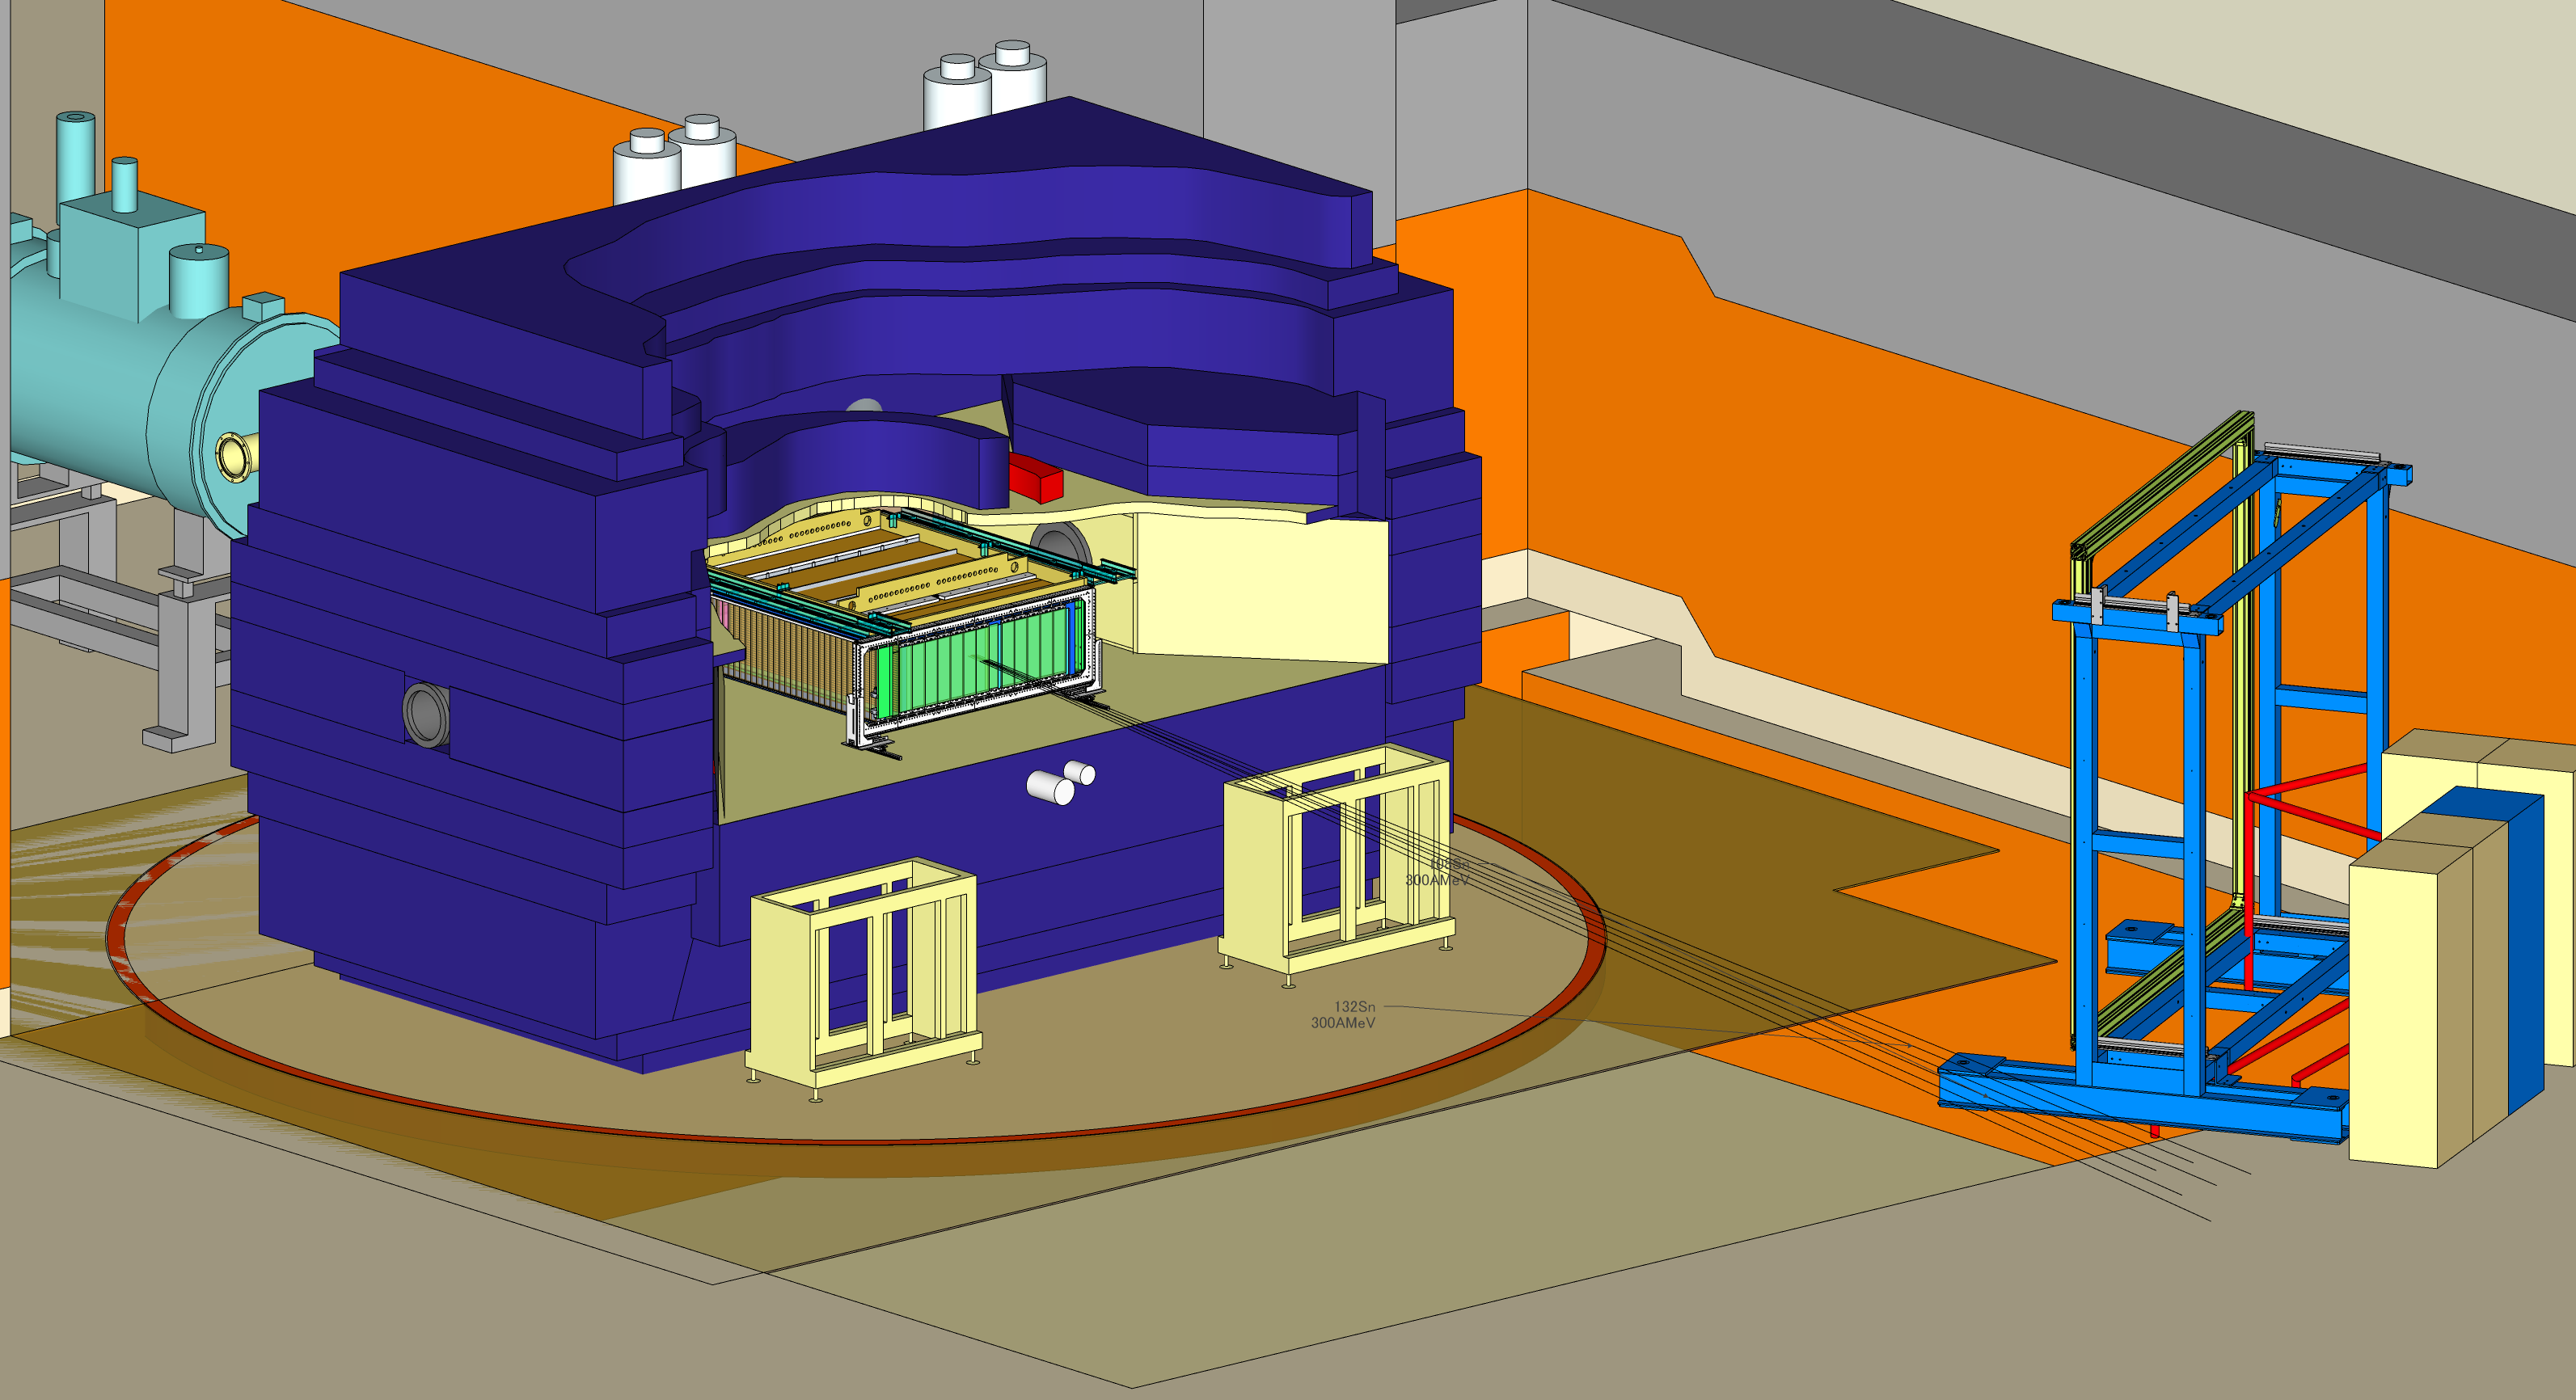
\includegraphics[width=\textwidth]{perspective.png}
\caption{Drawing of the experimental setup with the TPC inside of the SAMURAI magnet at $\ang{0}$ configuration.}
\label{fig:experiment}
\end{figure}

The height of the TPC was roughly aligned with a self-leveling laser system to match the center of target with the center of the beam line. Once the TPC was adjusted to the final location, the position of the TPC was measured in fine detail with a the VStars-N photogrametry system \cite{vstars}. Small highly reflective targets were placed all over the TPC both inside and out and pictures were taken with a calibrated lens and camera system. Using the commercial software provided the set of different camera perspectives was reconstructed into a 3-dimensional point cloud of all the targets. Since the magnet was also measured with the same system after installation, we can match the two systems to get the absolute position of the TPC, and its internal components, relative to the magnet frame. The position resolution of this type of system was estimated to be around \SI{200}{\micro\metre} for each coordinate.

The origin of the \spirit TPC was defined to be at the center of the TPC pad plane in the x-direction and at the edge of the first upstream pad. The center of the magnet is defined as the center of the magnet in x and z-directions and the middle of the dipole gap in the y-direction. The origin of the \spirit TPC in the magnet frame is (1.8,205.5,-580.5) for x,y,z-coordinates in units of \si{\milli\metre}. The error in each coordinate estimated to be (0.2,0.1,0.4) \si{\milli\metre} respectively. 

%Maybe put a position table summary here of the TPC position and definition of the coordinates system in the TPC frame and the Magnet frame

\section{Beam Drift Chambers (BDC)}
\label{sec:bdc}

There were two beam drift chambers (BDC) located along the beam pipe upstream of the magnet and after the last focusing quadropole magnet. These beam drift chambers contained two sets of parallel plate avalanche counters (PPAC) which could get the (x,y) coordinates of the beam. Since they were places approximately \SI{1}{\metre} apart, we were able to track the direction of the beam in the beam line using a linear extrapolation. The resolution of the initial angle the beam enters the SAMURAI dipole was estimated to be \SI{0.64}{\milli\radian} and \SI{0.24}{\milli\radian} for the two angles defining the beam vector \cite{jon}. The initial angle, energy, and charge of the beam is then propagated through the magnetic field map until the angle on target is found. The angle on target though small will be important later for transforming back into the center of mass system as will be seen in Section~\ref{sec:beamangle} and Section~\ref{sec:pionSpectra}.


\section{Ancillary Detectors }
Several ancillary detectors were placed inside and outside of the \spirit TPC to facilitate in making the trigger for the experiment. The ability of ancillary detectors to work effectively when placed outside the TPC  was one of the more important considerations we made when designing the TPC. A brief description of each ancillary detector system is given here with particular focus on how the experimental trigger was made. 


\subsection{Kyoto Multiplicity Trigger}
\label{sec:kyoto}
%kyoto array sets multiplicity trigger
%scintillator bars
 The Kyoto Multiplicity Array, shown in Figure~\ref{fig:aux}, consists of two arrays of plastic scintillating bars on each side of the TPC, each consisting of 30 bars. The entire TPC structure was designed so that light charged particles could pass through the field cage and side walls of the TPC enclosure without excessive energy loss and scattering. This allowed the number of tracks passing through the sides of the TPC could be measured by in an external array. In heavy ion collisions the more central a nuclear collision is, the more nucleons participate in the collision, resulting in a higher observed track multiplicity. It is this correlation between the number of tracks and centrality of the collision that makes the number of hits in the Kyoto Array sensitive to the centrality of events. It is more likely that in very central collisions more tracks are going to the large angles and measured by the Kyoto array. In the experiment the trigger selection criteria was $n_{Kyoto} > 4$, where $n_{Kyoto}$ is the total number of tracks measured by both arrays. The Kyoto array proved to be a good trigger that suppressed peripheral collisions; this will be discussed in later sections. 

\begin{figure}[!htb]
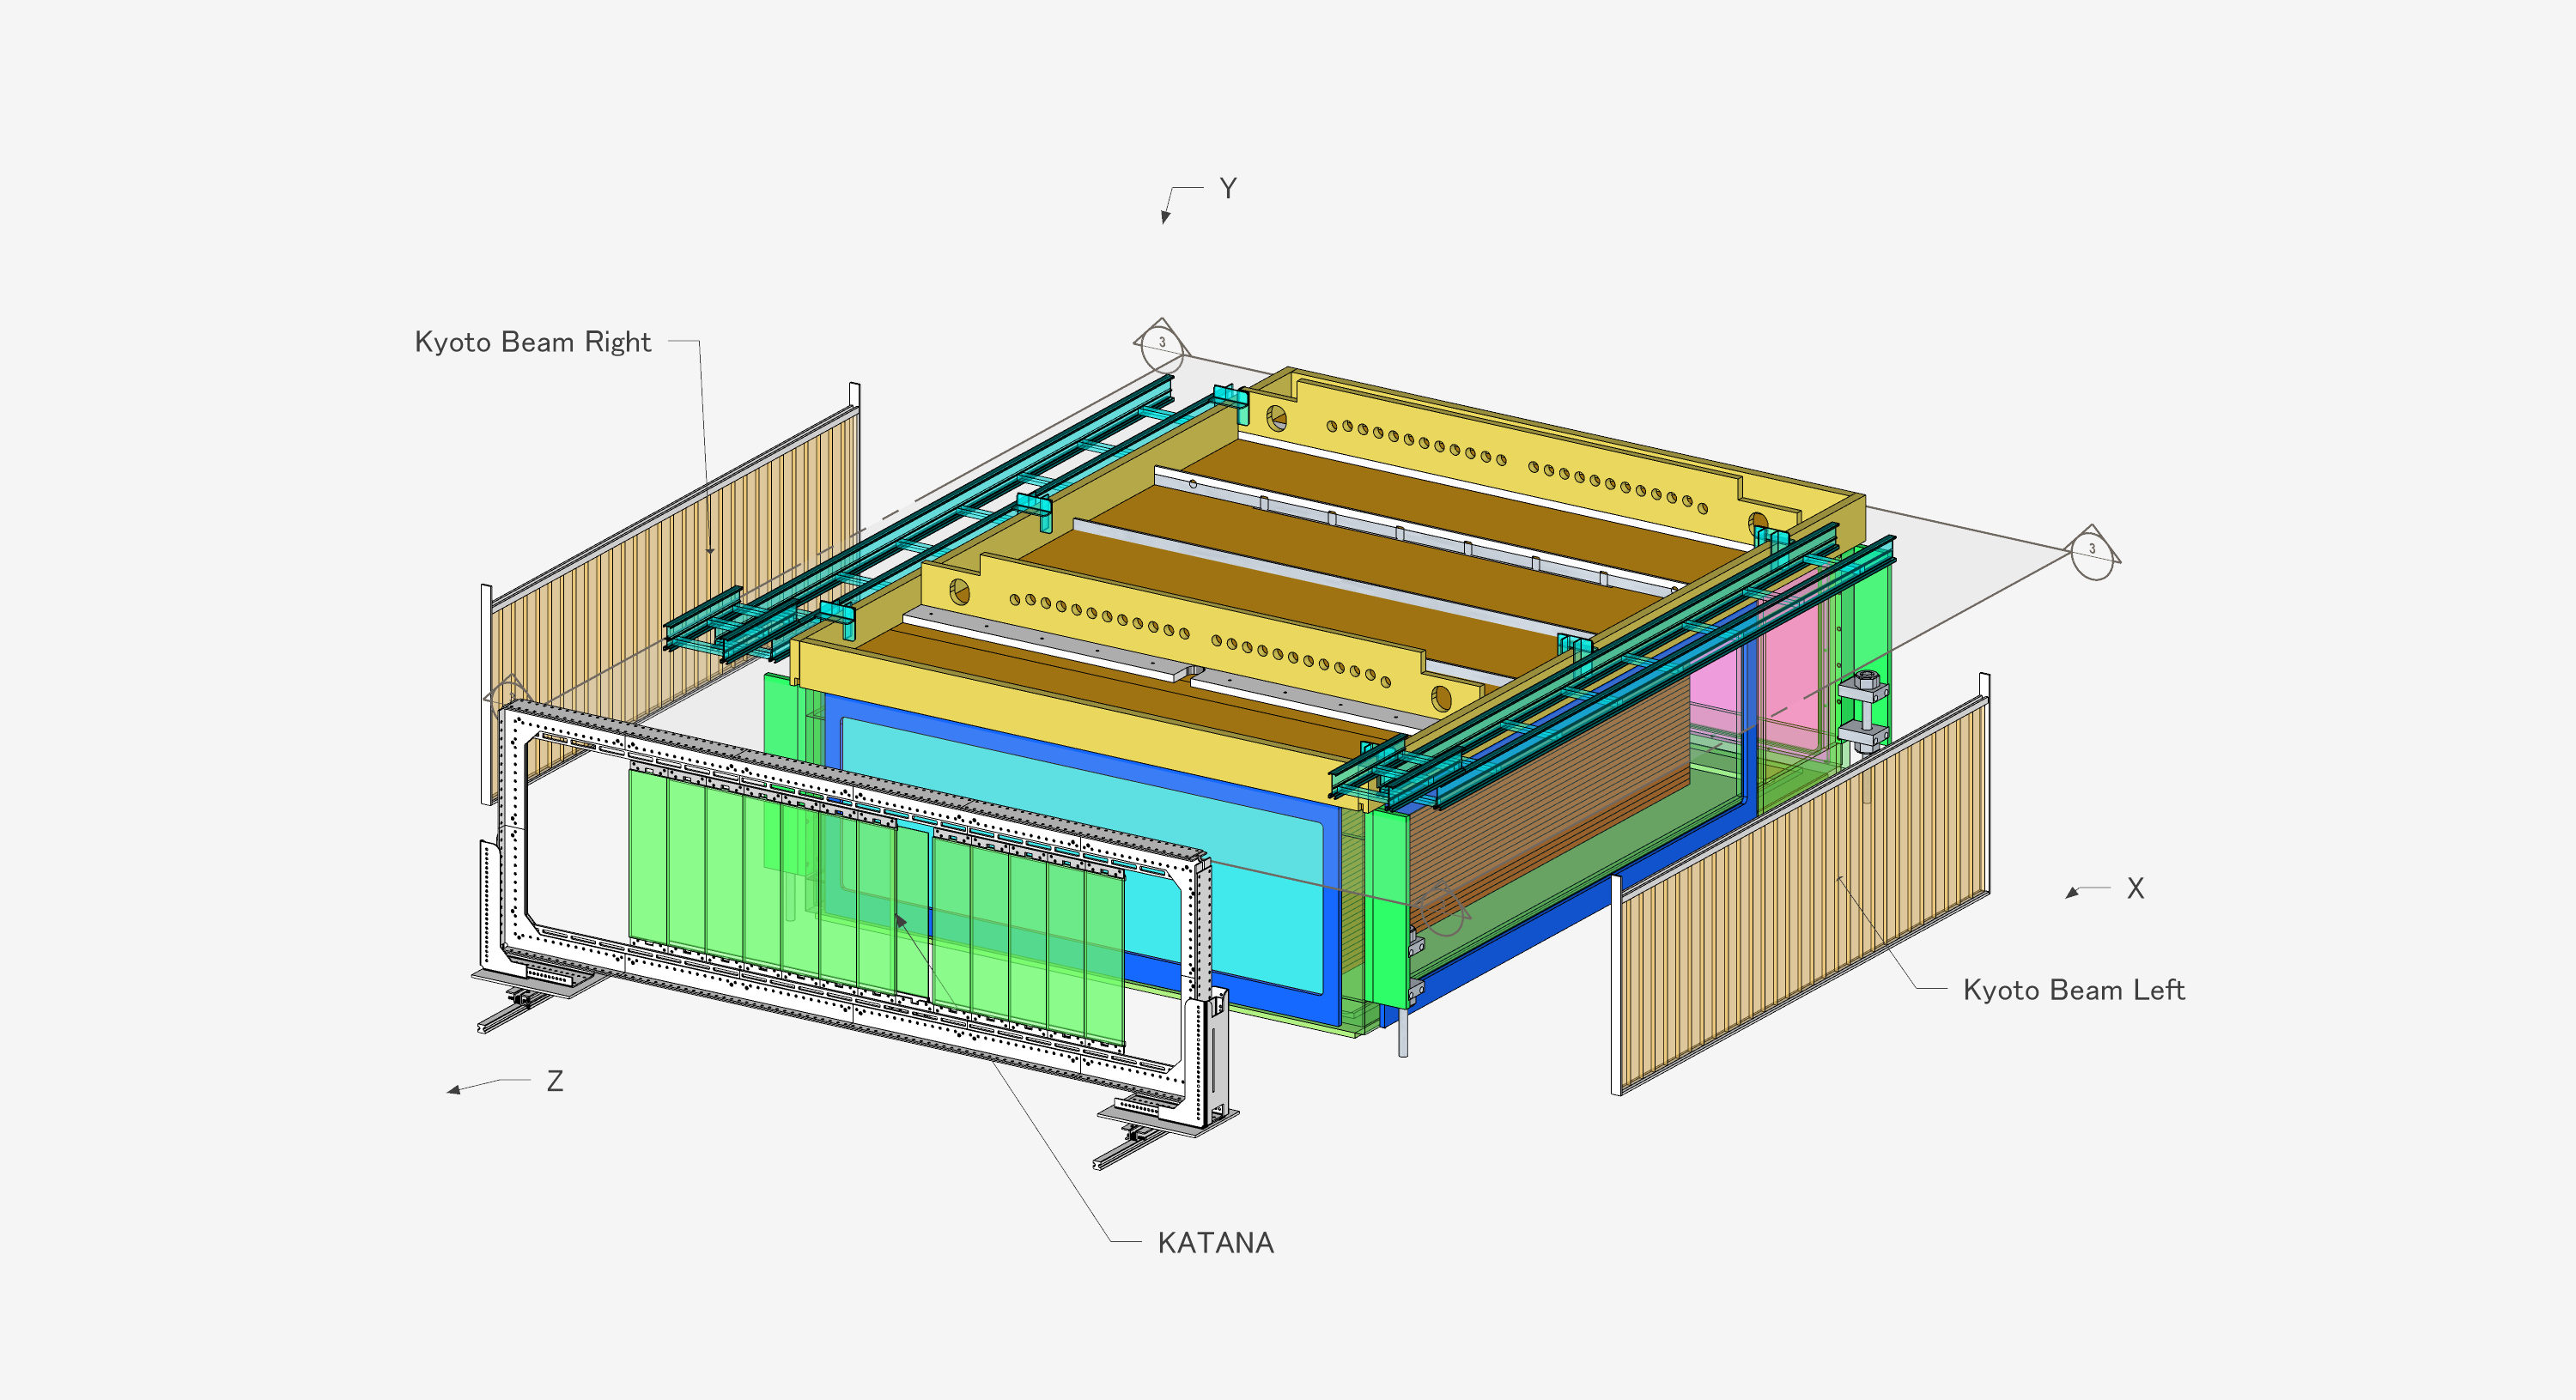
\includegraphics[width=\textwidth]{TPCAux.png}
\caption{Exploded views of Kyoto and KATANA arrays.The Kyoto array elements are in tan and are located on the left an right side of the TPC. When they are in place, they are nested against the thin Aluminum side windows of the TPC. The KATANA array is in green and is located adjacent to the downstream window of the TPC.}
\label{fig:aux}
\end{figure}


\subsection{KATANA Veto and Multiplicity Array}
%beam veto
%beam trigger optional
 Figure~\ref{fig:aux} also shows the Krakow KATANA array, which consists of 12 plastic scintillating bars mounted adjacent to the downstream wall of the TPC enclosure. Three of the 12 bars, which are 1 mm in thickness, and operated as a beam veto in the event the beam did not make a nuclear collision with the target; this occurred approximately 99\% of the time. The 9 other bars were 1 cm in thickness and provided additional information about the light particle multiplicity array similar to the Kyoto array. We found that a large number of events involved peripheral collisions and active target events in which the beam interactions with the counter gas. Active target events contributed to a large multiplicity in the KATANA but not to the Kyoto array. So multiplicity $M_{Kyoto} > 4$ in the Kyoto array combined with a veto on events with a forward going projectile remnant with Z>20 provided the most effective suppression of peripheral collisions and active target events. Thus the KATANA array was used in primarily the beam veto mode. This was accomplished by positioning the array so that the expected position of the beam exiting the TPC would be centered on the three thin paddles. The threshold of the veto paddles were set so that the charge of a particle passing through, $Z$, would veto any event that satisfied $Z > 20$, where the charge of the Sn beam is $Z=50$. 


\subsection{Active Veto Array}
The beam was tuned by two sets of quadrupole  magnets, STQ 1 and STQ2 (as seen in Figure~\ref{fig:samuraiBeamLine}), so that the beam spot was focused on the TPC target location. Because of the inherent angular dispersion of the beam, some events significantly deviated from the target location. These could be suppressed in the analyses by a gate on the reaction vertex; however, there remained a concern about the dead time such target frame events would contribute and how this would limit the amount of good data we could obtain.  To veto these type of events an active veto array was set at the entrance of the TPC consisting of four small scintillating bars arranged to be slightly larger than the target size. The threshold was set so that any beam particle which passed through any of the bars it would send a signal not to trigger the system since the beam path would not be on target but on some other material inside the TPC. Minimizing these active veto rates also proved to be useful when tuning the beam to be more centered on the target.


\section{Data Acquisition (DAQ) }
The Data AcQuisition (DAQ) consisted of three different systems. The RIBFDAQ system served as the master DAQ for the BigRIPS beam identification DAQ, the TPC DAQ, the NeuLAND neutron wall DAQ, and the Kyoto Array DAQ systems. The TPC DAQ was handled by the NARVAL framework to readout the GET electronics for the \spirit TPC. A General Trigger Operator (GTO) trigger was supplied to each DAQ synchronizing the subsystems. 

\section{Trigger Condition}
Signals from all of the auxiliary detectors were combined into several logic combinations to form a trigger logic for triggering the data acquisition  (DAQ) to record data. An upstream scintillating bar formed the start counter signal, triggering on any beam coming down the beam line. The active veto will trigger for any beam that is off the target location. The KATANA veto produced a signal if the beam passed through the TPC un-reacted, causing no nuclear collision; this produces a veto signal with a width of \SI{4}{\micro\second} which is the approximate time it takes for the beam to drift and clear the field cage volume. The Kyoto multiplicity trigger produces a signal when the total number of tracks passing through both Kyoto arrays are greater than 4. 


\begin{figure}[!htb]
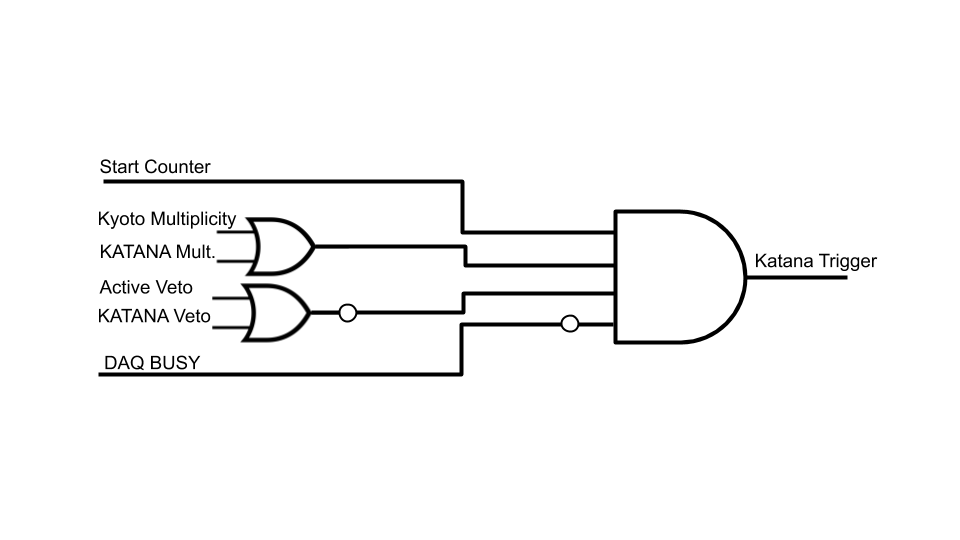
\includegraphics[width=\linewidth]{KatanaLogic.png}
\caption{KATANA trigger box logic.}
\label{fig:katanaLogic}
\end{figure}

\begin{figure}[!htb]
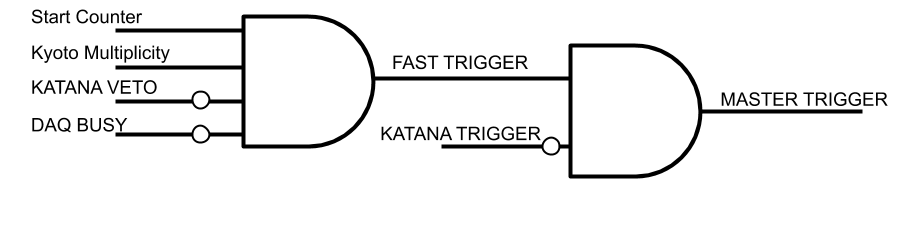
\includegraphics[width=\linewidth]{TriggerLogic.png} 
\caption{Master trigger logic.}
\label{fig:trigLogic} 
\end{figure}

\begin{figure}[!htb]%
    \centering
    \subfloat[${}^{124}$Xe primary beam trigger.]{{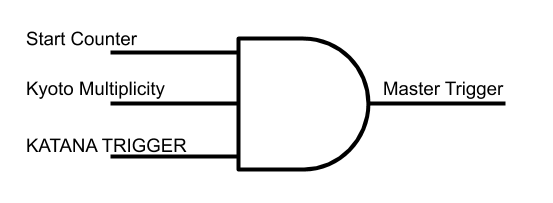
\includegraphics[width=.45\textwidth,valign=t]{DataTrigger1.png} \label{fig:dataTrigger1}}}%
    \qquad
    \subfloat[${}^{238}$U primary beam trigger.]{{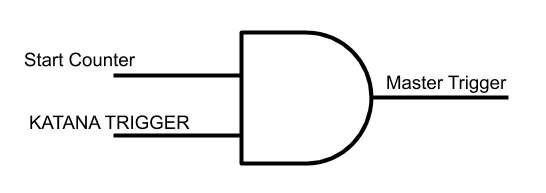
\includegraphics[width=.45\textwidth,valign=t]{DataTrigger2.png} \label{fig:dataTrigger2}}}%
	\caption{Master triggers in each primary beam setting.}    
	\label{fig:datatrigger}
\end{figure}

There were several special trigger considerations incorporated into the trigger for the TPC. We required that the gating grid be opened quickly to not lose electrons from portions of the tracks that pass close to the gating grid. If the DAQ was not busy, we therefore generated a trigger once we had a start detector signal, a Kyoto multiplicity >4 signal, and neither a Katana Veto signal nor an active target signal. This was referred to as the Fast Trigger, and it triggered the opening of the gating grid, which took about 350 ns. Following the initial trigger, we had the possibility of a fast clear signal that could be initiated by a later beam particle traversing the TPC. If the last beam particle came within 4 us after the fast trigger, electrons from this beam particle could pass through the gating grid. Such data would be useless, so we closed the gating grid and stopped the data acquisition with a fast clear signal. Additional fast clears  also was initiated if the Katana trigger box did not generate a trigger. Figure~\ref{fig:trigLogic} shows the logic of both of these triggers.

The Katana trigger box initially did not take on the major trigger responsiblities. In later runs, most of the trigger functions were performed in the Katana trigger box. The master trigger for the DAQ was different for each primary beam. During the ${}^{124}$Xe primary beam, the KATANA trigger box was an input into the trigger logic, whereas in the ${}^{238}$U primary beam, the KATANA trigger box functioned as the trigger logic utilizing the internal trigger electronics. In either case the differences in the trigger logic were very minor and they both behaved practically the same except for minor details on the gating-grid trigger \cite{jon}. Figure~\ref{fig:katanaLogic} summarizes the KATANA trigger box logic. 

Figure~\ref{fig:dataTrigger1} summarizes the ${}^{132}$Xe primary beam, where the condition to produce a true KATANA trigger output required a Start Counter, KATANA multiplicity, no Veto, and no DAQ busy signal. The KATANA trigger, Kyoto Multiplicity, and Start Counter together triggered the DAQ. 

 Figure~\ref{fig:dataTrigger2} summarizes the ${}^{132}$Xe primary beam, where the condition to produce a true KATANA trigger output required a Start Counter, Kyoto or KATANA multiplicity, no Veto, and no DAQ busy signal. Here the KATANA trigger and the SC SUM together triggered the DAQ. 
 
 %I don't think this is true.
 
 It is worth mentioning how the busy signals for the experiment were handled. The DAQ system itself produces a busy signal which was combined in an OR with the busy signals from either the opening or closing the gating grid. When opening the gating grid, it is assumed the full volume of the TPC will be read out, therefore  a \SI{11}{\micro\second} gate busy signal is produced; which is slightly more than the time it takes for all the electrons to drift in the field cage. In the case where the gating grid should be closed, either due to the fast clear circuit or the end of the TPC measurement, a \SI{5}{\micro\second} busy signal is produced to allow for the gating grid to settle to a steady state, closed configuration, and to clear the drift volume of any residual electrons from the beam. Both of these gates are included with the DAQ in an OR configuration which makes the overall busy signal. 
 


\section{Collision Data}

Figure~\ref{fig:data} shows the example pad plane readout of the TPC from a central nuclear collision of Sn + Sn. Here we can see several tracks resulting from a single vertex location which is near the target region. The color values represent the max ADC observed in a given pad. The large amount of saturation that occurs in the electronics which is represented by the brightest yellow value. Also the lower voltage anode sections described in Section~\ref{sec:wireplanes} are denoted by red arrows. The pads directly over these wire planes have an effective gain reduction due to the lower anode voltage on the wires. Tracks with a high enough energy loss continue through these sections, but tracks with low energy loss values do not deposit enough energy and disappear, only to reappear in the higher gain section in between. 

\begin{figure}[!htb]
\centering
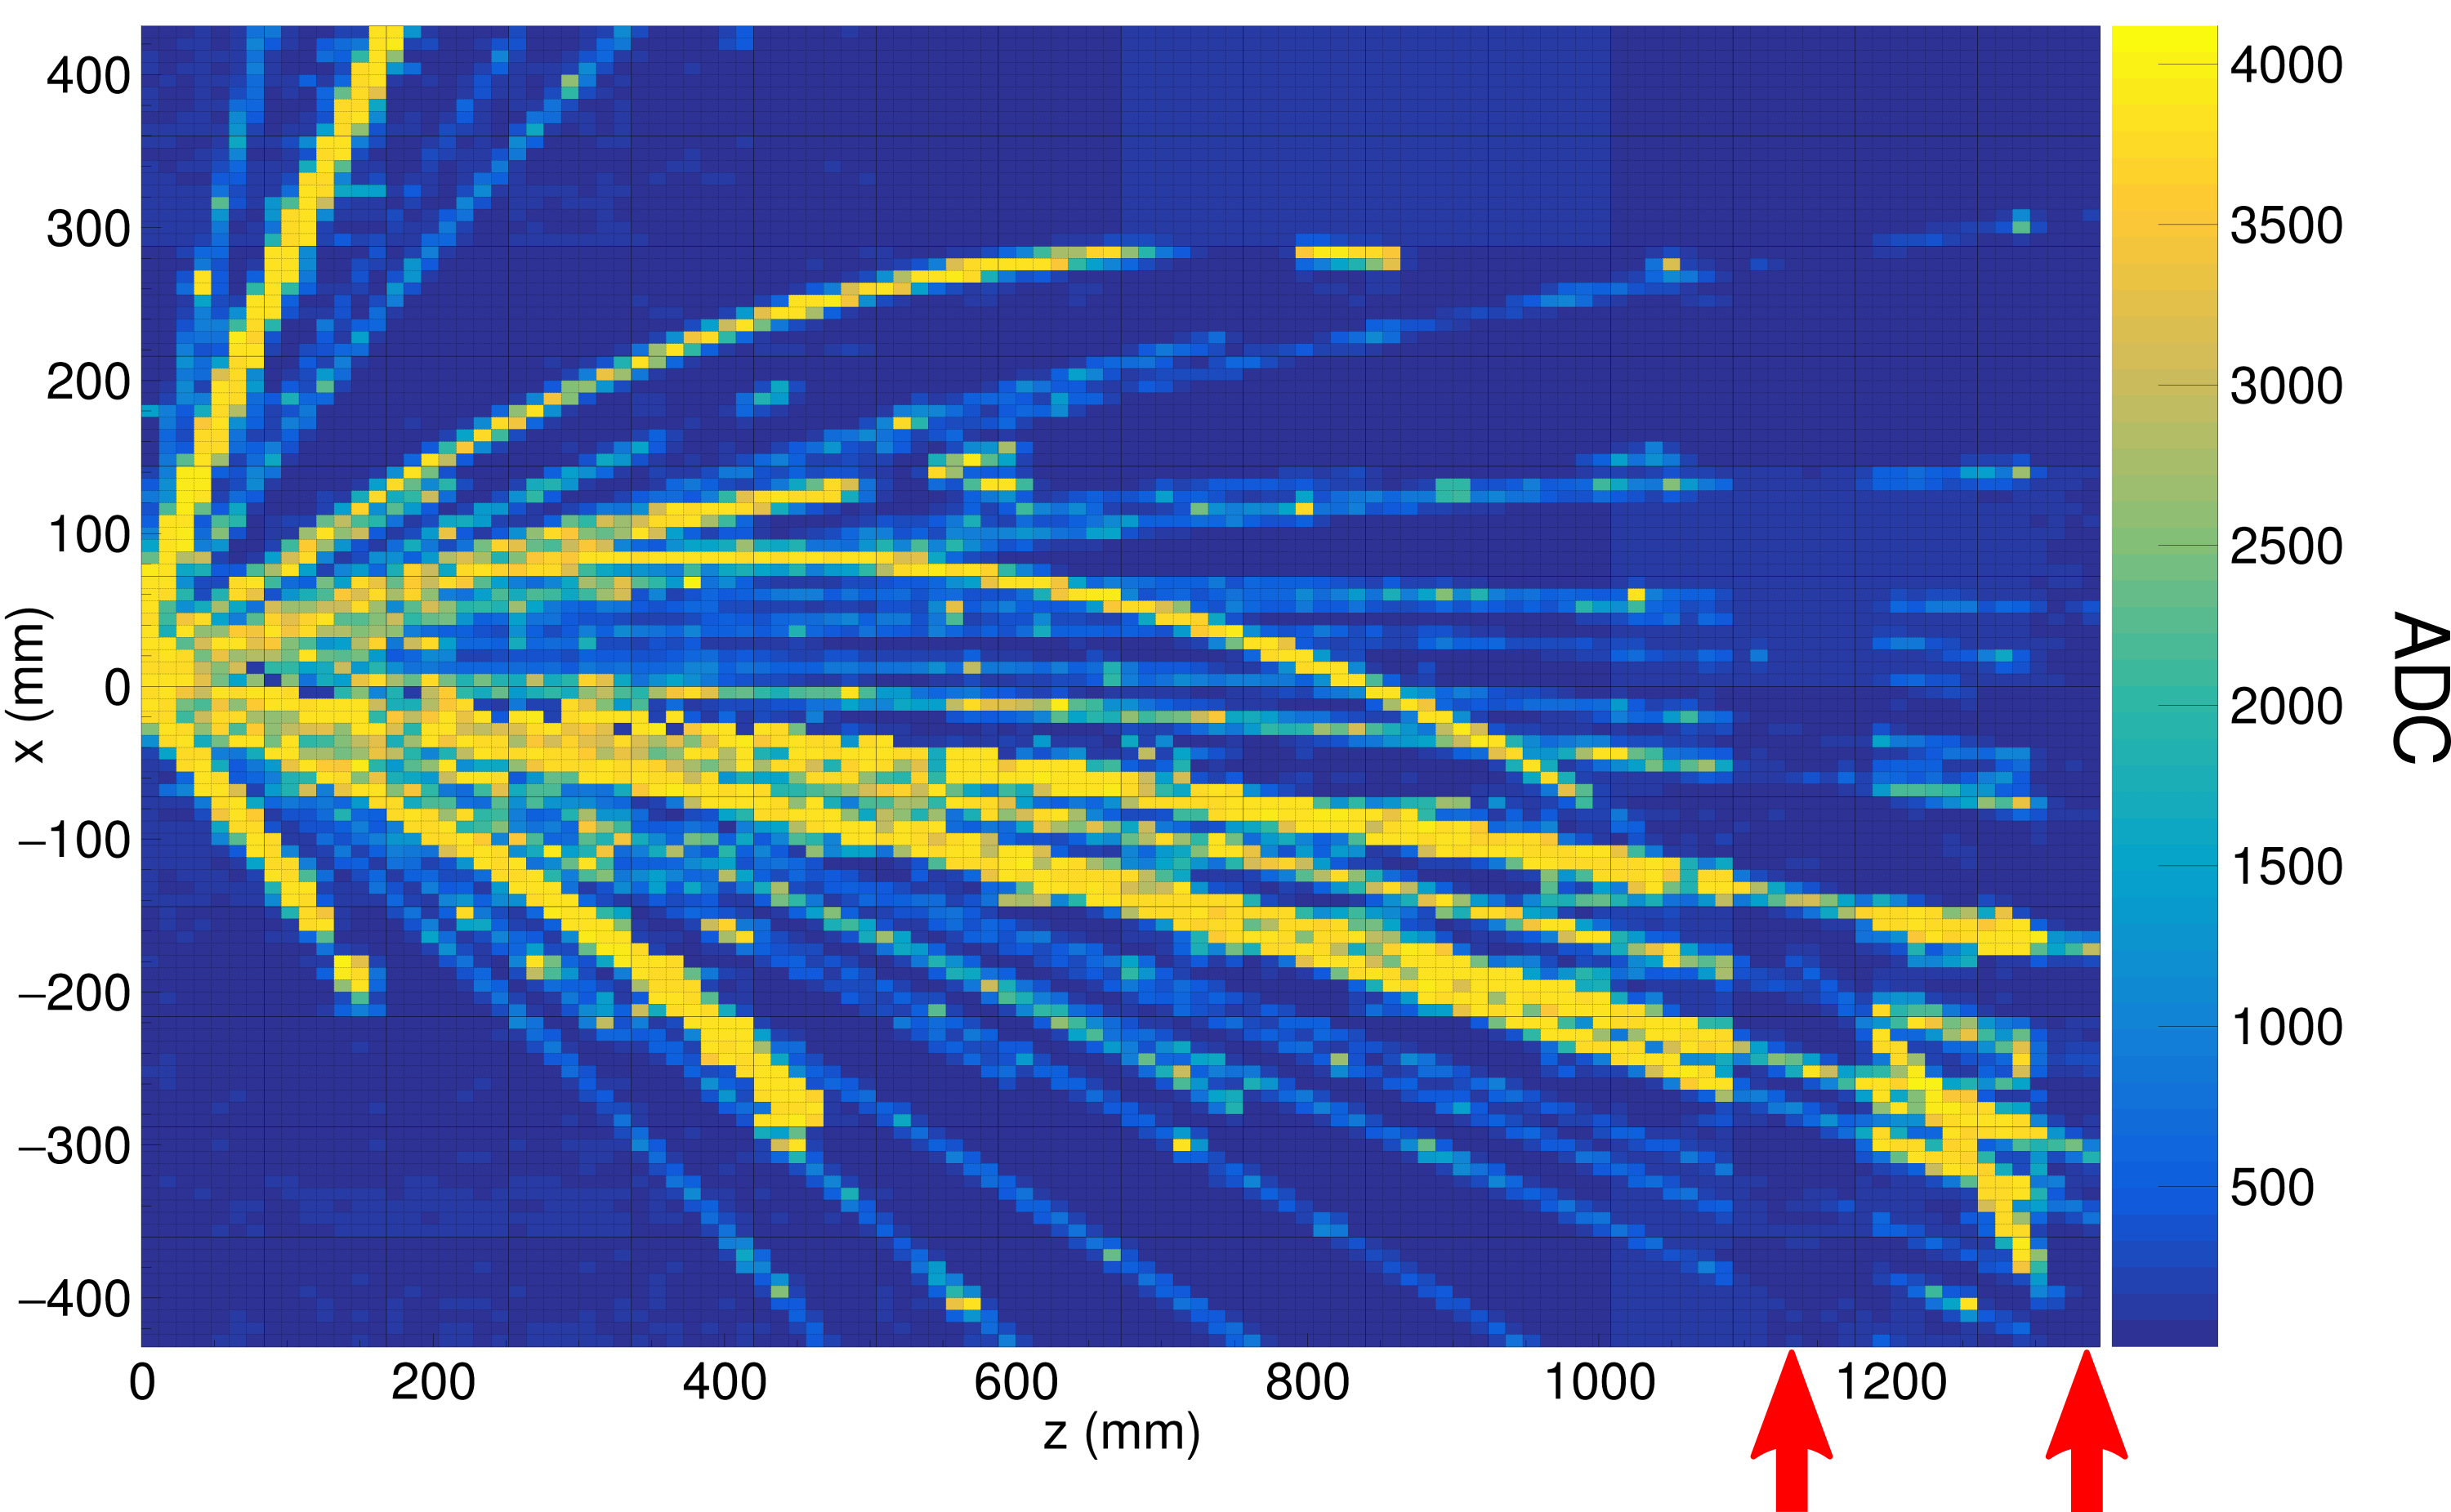
\includegraphics[width=.8\linewidth]{data.png}
\caption{Pad plane projection for a collision event in the TPC. Highlighted by red arrows are two regions of anode wires which had a reduced voltage of 1214 V. The voltage of the rest of the TPC anode wires are 1460 V. The reduction in voltage reduces the gain by a factor of about 10. }
\label{fig:data}
\end{figure}



Shown in Figure~\ref{fig:cocktail} is a typical calibration event, where one particle enters the TPC volume at a time and parallel to the pad plane, representing an ideal case for momentum and $dE/dx$ determination; as it does not suffer from inefficiencies of high multiplicity events seen in the collision experimental data. The primary goal of this data set was to calibrate the TPC in both momentum and dE/dx as will be discussed in Section~\ref{sec:cocktail}. 

\begin{figure}[!htb]
\centering
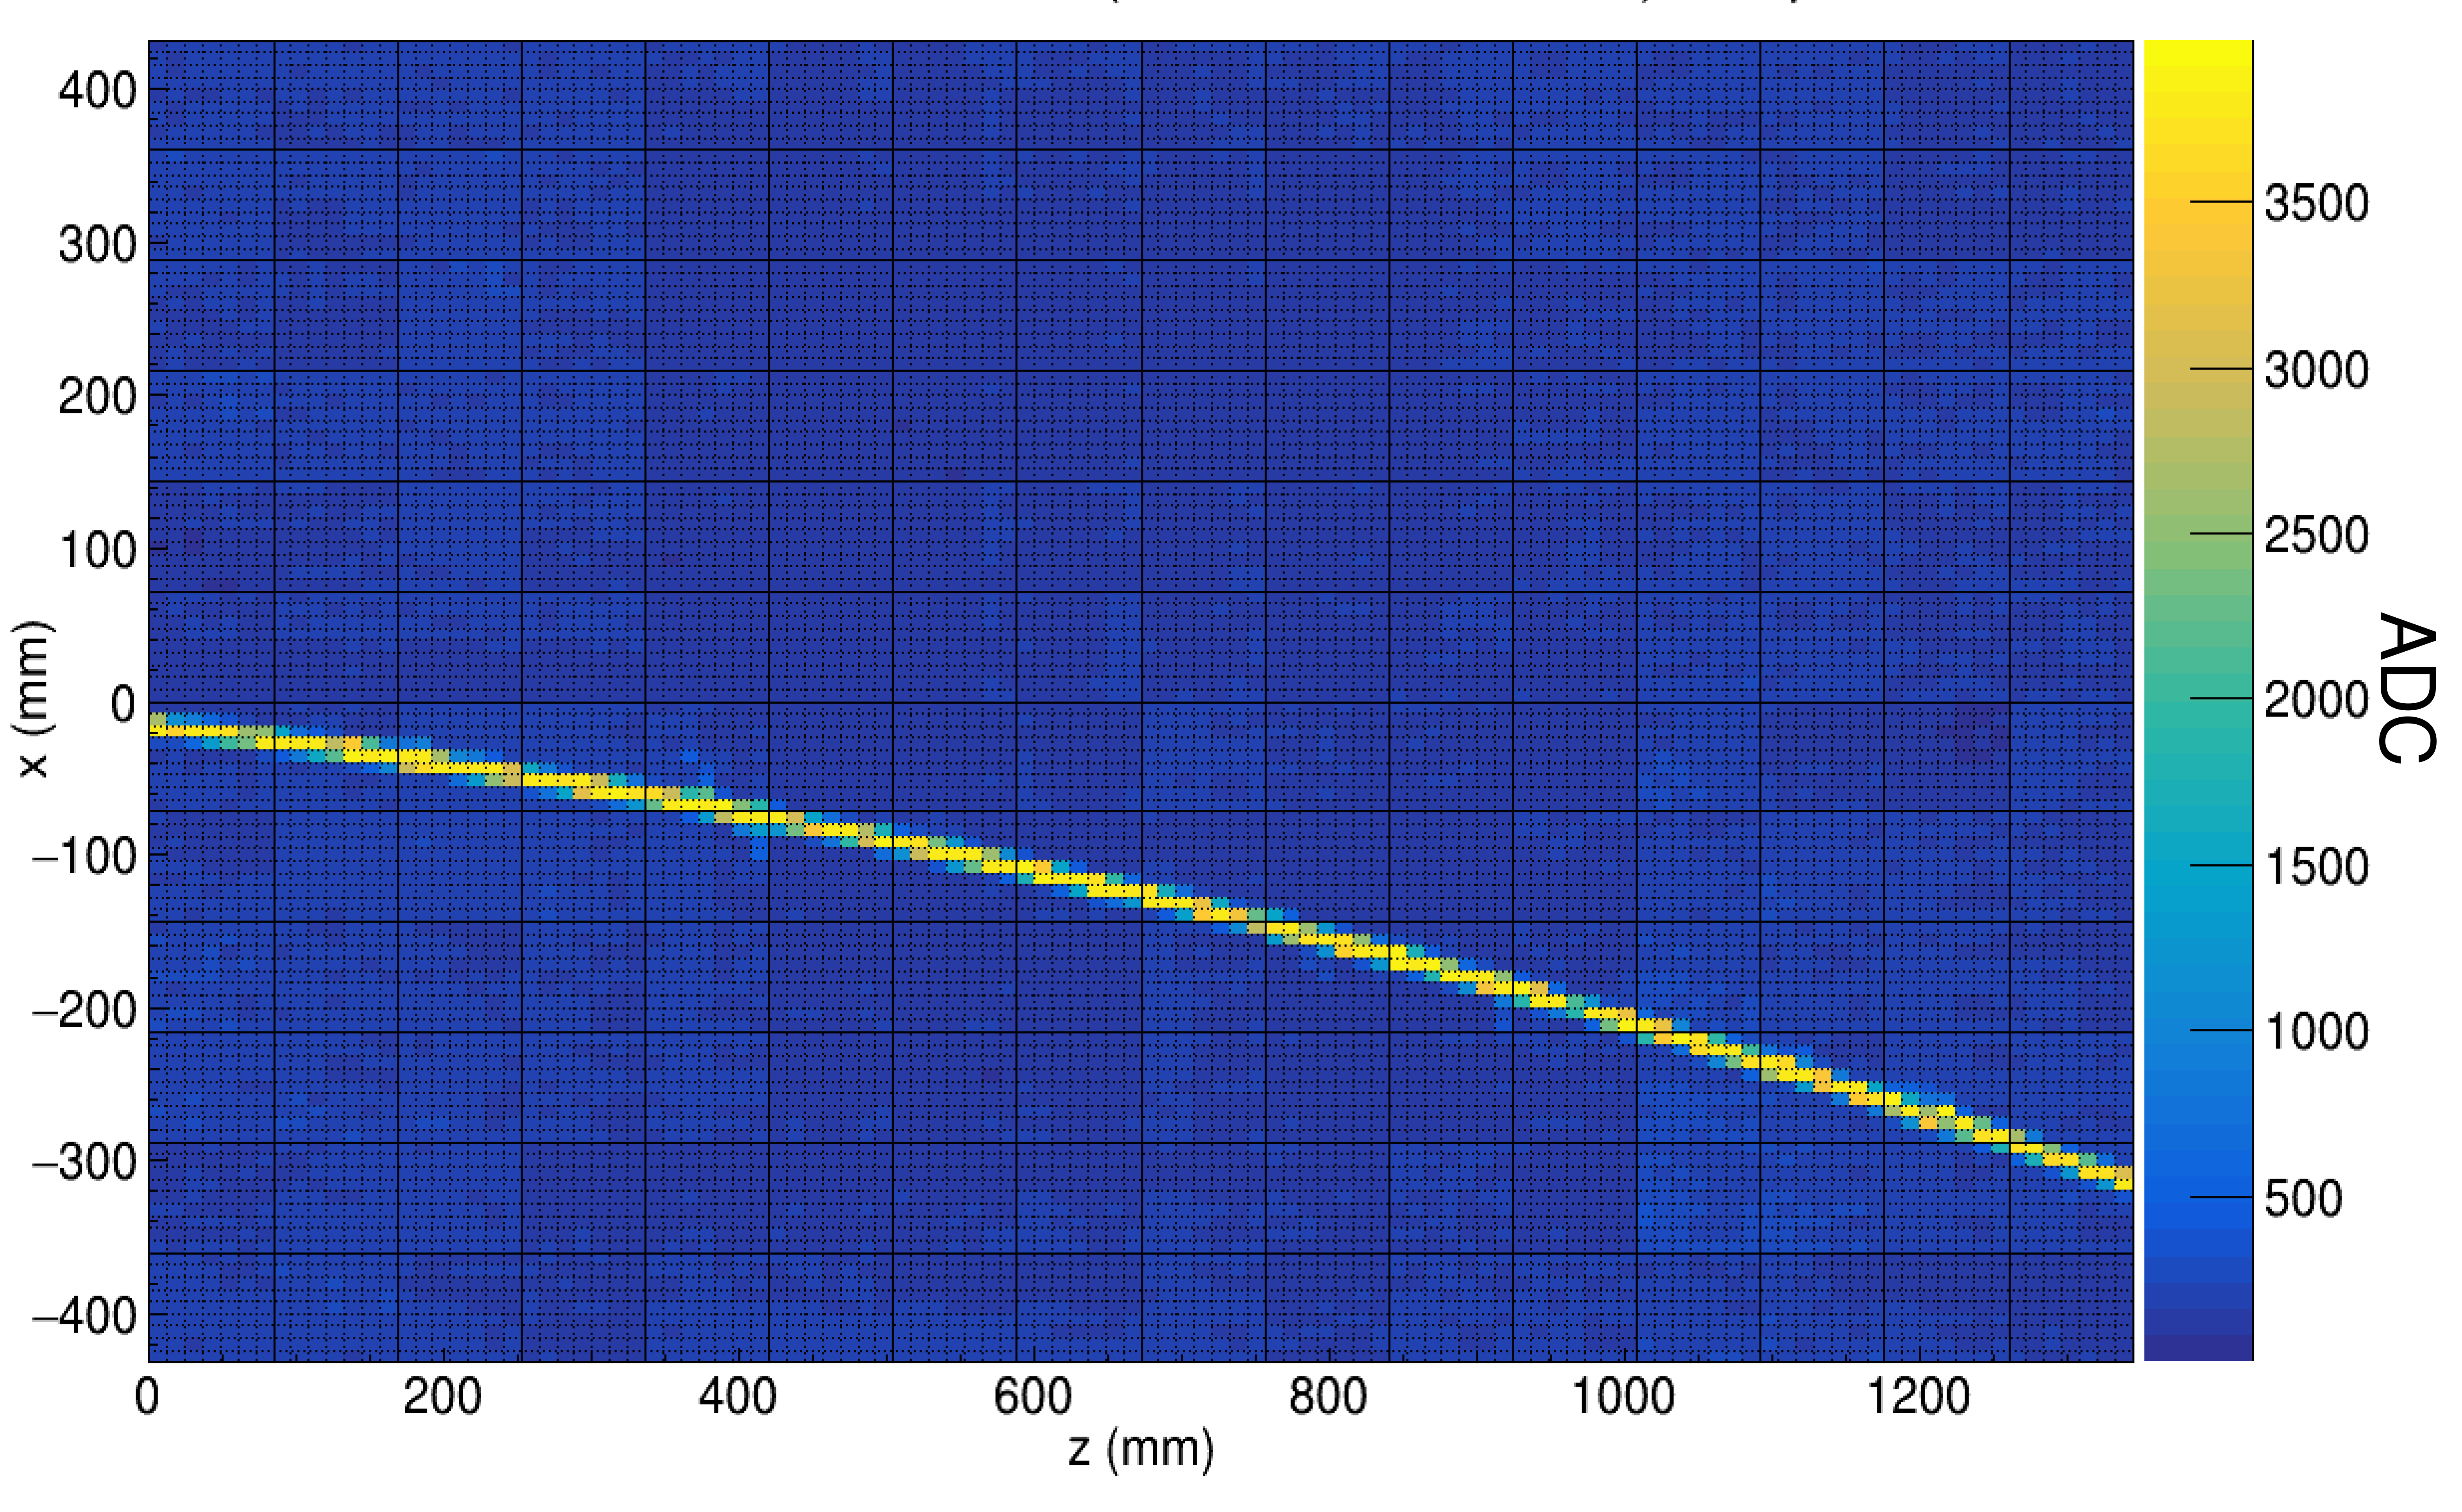
\includegraphics[width=.8\linewidth]{cocktail.png}
\caption{Pad plane projection for a calibration event in the TPC.}
\label{fig:cocktail}
\end{figure}



\chapter{Data Analysis I: Calibration and Corrections}
\label{chap:data1}

\section{S$\pi$RITROOT Software}
\label{sec:software}

The S$\pi$RITROOT software is written in c++ and is based on the FAIRROOT package \cite{fairroot}. It is separated into modules which can be turned on or off depending on the particular analysis. While the base classes and frame work are provided by the FAIRROOT package, we added the specifics of the \spirit TPC and the algorithms for track reconstrucition. Here we will briefly describe the outline of the main tasks in the S$\pi$RITROOT software and then will discuss of each task later. The level of discussion concerning the software is really a practical, base understanding, appropriate for the discussion of this dissertation. For more details about the tracking algorithm the reader is refered to \cite{spiritroot_paper}, and to actual software which is published on GitHub \cite{spiritroot_git}. 

The main tasks which make up the reconstruction algorithm are:

\begin{itemize}
  \item Decoder task
  \item Pulse Shape Algorithm (PSA Task)
  \item Helix Track Finding Algorithm
  \item Track Fitting and momentum reconstruction(GENFIT package)
  \item Vertex Reconstruction (RAVE package).
\end{itemize}


\subsection{Decoder task}
The decoder task reads in the raw data files output from the GET electronics converting the binary data into \spirit ROOT classes using the GETDecoder \cite{getdecoder}. When the software is loaded, a map is also loaded which maps each channel in the CoBo board onto the physical pad location on the pad plane. The information is stored in a pad container called the \emph{STPad} class. This container stores the row, layer, and the raw ADC time bucket spectrum; where the row refers to the pad numbering along the x-direction and the layer refers to the numbering along the z-direction. Then the information from all of the pads is combined to form the event container called the \emph{STRawEvent} class which represents the raw event information. 

Three basic calibrations are performed on the raw data level within this task. The gain calibration calibrates the electronics will be described in Section\ref{sec:elecCalib}. The anode gain calibration which will be discussed in Section~\ref{sec:anodeCalib}, and the gating grid noise subtraction and time bucket cut which is described in Section~\ref{sec:ggnoisesub}.
%gain calibration 
%ggnoise subtraction
%GG time bucket cut


\subsection{Pulse Shape Algorithm (PSA) Task}
\label{sec:psa}
%Yoffset match the TPC-Vertex_y with BDC_Y
%YPedestalOffset what is it for?
%cobo gain matching
An algorithm loops over the raw time bucket spectrum to find all the unique pules in each pad. It is very likely that there are several pulses in a pad coming from multiple tracks passing under the same pad which are separated only in arrival time. Figure~\ref{fig:psaTask} shows the PSA task working on one particular pad in experimental data. The shaded histogram in every sub-figure represents the ADC raw spectrum of the pad. In Fig.~\ref{fig:psa0} we see the PSA has identified the first pulse and fitted it with the standard pulse; the result of the fit is shown by the red line. The fitted red line is then subtracted from the ADC spectrum, which is shown in the shaded histogram in Fig.~\ref{fig:psa1}. Here, the second pulse is found and fitted again with the same procedure; the red line will be subtracted from the raw ADC spectrum. The black line represents the sum of all the fitted pules in each step. This continues until all pules are found or until the PSA reaches the last bin in the spectrum. Figure~\ref{fig:psa4} shows the final result where 4 fitted pulses were found. The agreement between the total summed line and the raw ADC spectrum exemplifies how successful the PSA is in this particular set of data. 

%Mention about the minimum distance between hits? 

The fit of each individual pulse contains the height of the pulse and the timing information of the start of the pulse. We define the start of the pulse to be the location in time when the rising edge of the pulse reaches of 10\% of its peak value. The height of the pulse is related to the charge induced on the pad, $Q$. Combined with the start time of the pulse $t_o$  it is saved into a new container representing a \emph{hit}, called the \emph{STHit} class. After the PSA processes each pad in the raw event, an entire hit cloud of the event is produced. The x and z-coordinates come from the center of the pad which is already stored in the map of STPad. Since the STHit class inherits from the STPad class this information is also carried over. The y-coordinate is calculated using the known drift velocity $v$ and time of the signal $t_o$ as $y = v\cdot t_0$, $t_0$. The hit class forms the fundamental structure from which all tracking is performed since it contains the x,y,z spacial coordinates, and charge information $Q$.

\begin{figure}[!htb]%
    \centering
    \subfloat[$\mathrm{1^{st}}$ step of the PSA]{{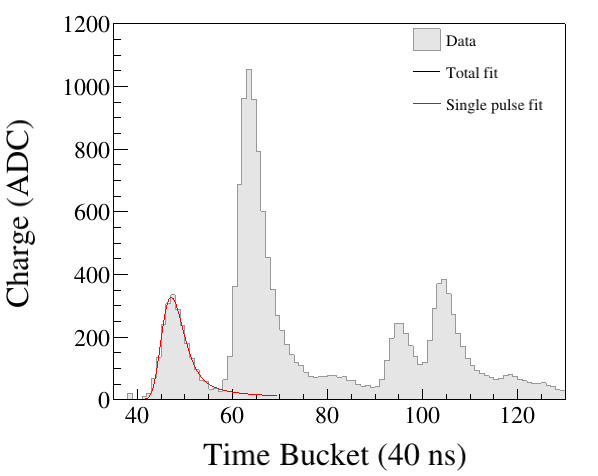
\includegraphics[width=.4\textwidth,valign=t]{psa0.png} \label{fig:psa0}}}%
    \qquad
    \subfloat[$\mathrm{2^{nd}}$ iteration]{{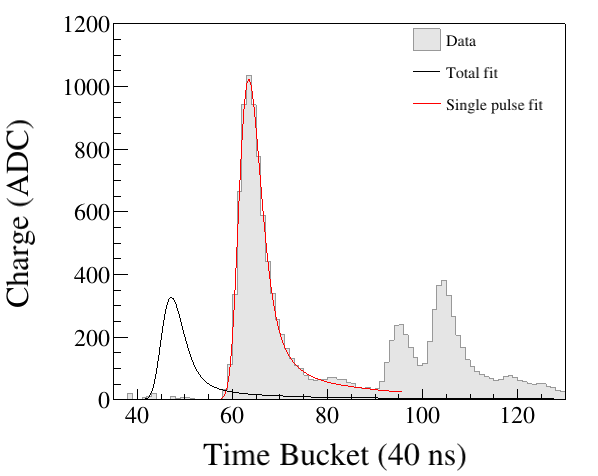
\includegraphics[width=.24\textwidth,valign=c]{psa1.png} \label{fig:psa1}}}%
    \subfloat[$\mathrm{3^{nd}}$ iteration]{{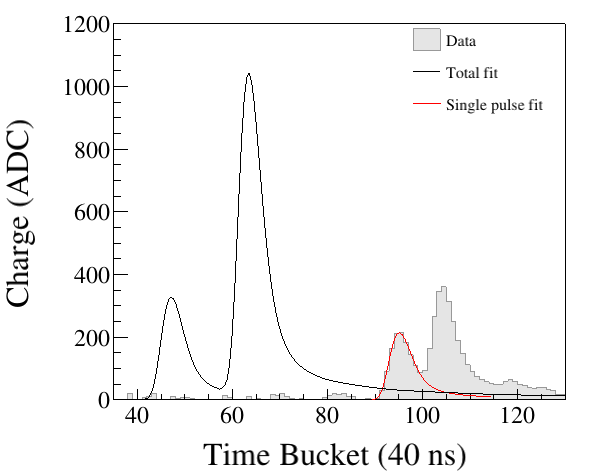
\includegraphics[width=.24\textwidth,valign=c]{psa2.png} \label{fig:psa2}}}%
    \subfloat[$\mathrm{4^{nd}}$ iteration]{{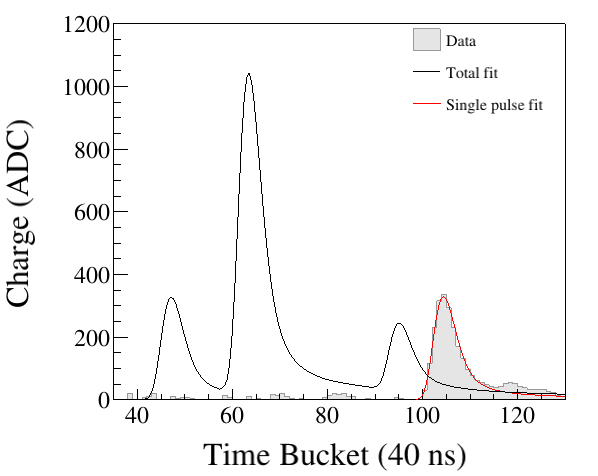
\includegraphics[width=.24\textwidth,valign=c]{psa3.png} \label{fig:psa3}}}%
    \subfloat[Final output of the PSA]{{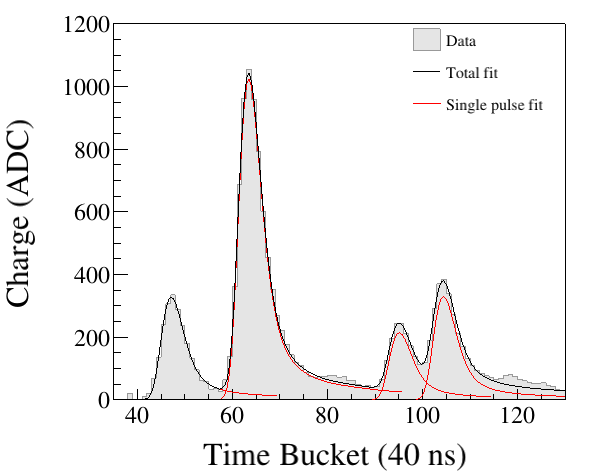
\includegraphics[width=.24\textwidth,valign=c]{psa4.png} \label{fig:psa}}}%

  	\caption{Example of the pulse shape algorithm through each step of in processing a given pad. }
	\label{fig:psaTask}
\end{figure}


\subsection{Helix Tracking}
%Cluster cut
%ellipsoid cut
\label{sec:helixtrack}

 The function of the  helix track finding algorithm is to sort the hit cloud into unique sets of hits representing tracks. This is performed by a Riemann track finding algorithm where the Cartesian space is mapped onto a Riemann sphere. This is a particular transformation in which unique helices in the Cartesian space form great circles on the Riemann sphere. This is particularly useful since hits which correspond to a track form a helices the Cartesian space of the TPC coordinates. It is difficult to search for tracks in the hit cloud by fitting a general helix to different combinations of hits. It is much easier to search for collection of hits by fitting a plane to the great circles which are formed on the Riemann sphere. More details on the Riemann tracking can be found here \cite{spiritroot_paper}. From here the set of hits which form a unique track are stored into a new helix track container called the STHelixTrack class. 
 

%\paragraph{Definition of clustering}
The hits within a helix track are dense and the position resolution of an individual hit is not very precise. As discussed in Section~\ref{sec:prf}, the TPC achieves sub-millimeter position resolution by combining neighboring pads into clusters using the the Pad Response Function (PRF). In the helix track finding task, the hits are further reduced into more precise clusters. A brief description of the method of clustering is illustrated in Figure \ref{fig:topview}. We have found that it is sufficient to simply cluster hits along one direction, either along the x or z-direction, depending on which direction is most perpendicular to the track. For example, the three clusters at the bottom of Figure \ref{fig:topview} are clustered along the x-axis, and the upper three are along the z-axis. The bold pads highlight the hits belonging to an example cluster from each set. Since we decide to cluster only in one direction, there is a natural inflection point in a track where the direction of clustering must switch. This switching point is determined by the crossing angle of the track $\theta$, which is defined as the angle between the tangent of the track, projected onto the pad plane, and the x-axis -- at a particular cluster location. In this definition, $\theta = \ang{90}$ corresponds to the case when the track is going along the z-axis and $\theta = \ang{0}$ for a track going along the x-axis.  The clustering direction in the case $\ang{45} < \theta \leq \ang{90} $ is along the x-direction. For tracks with angles $\ang{0} < \theta \leq \ang{45}$ we cluster along the z-axis. 

 

\begin{figure}[!htb]
\centering
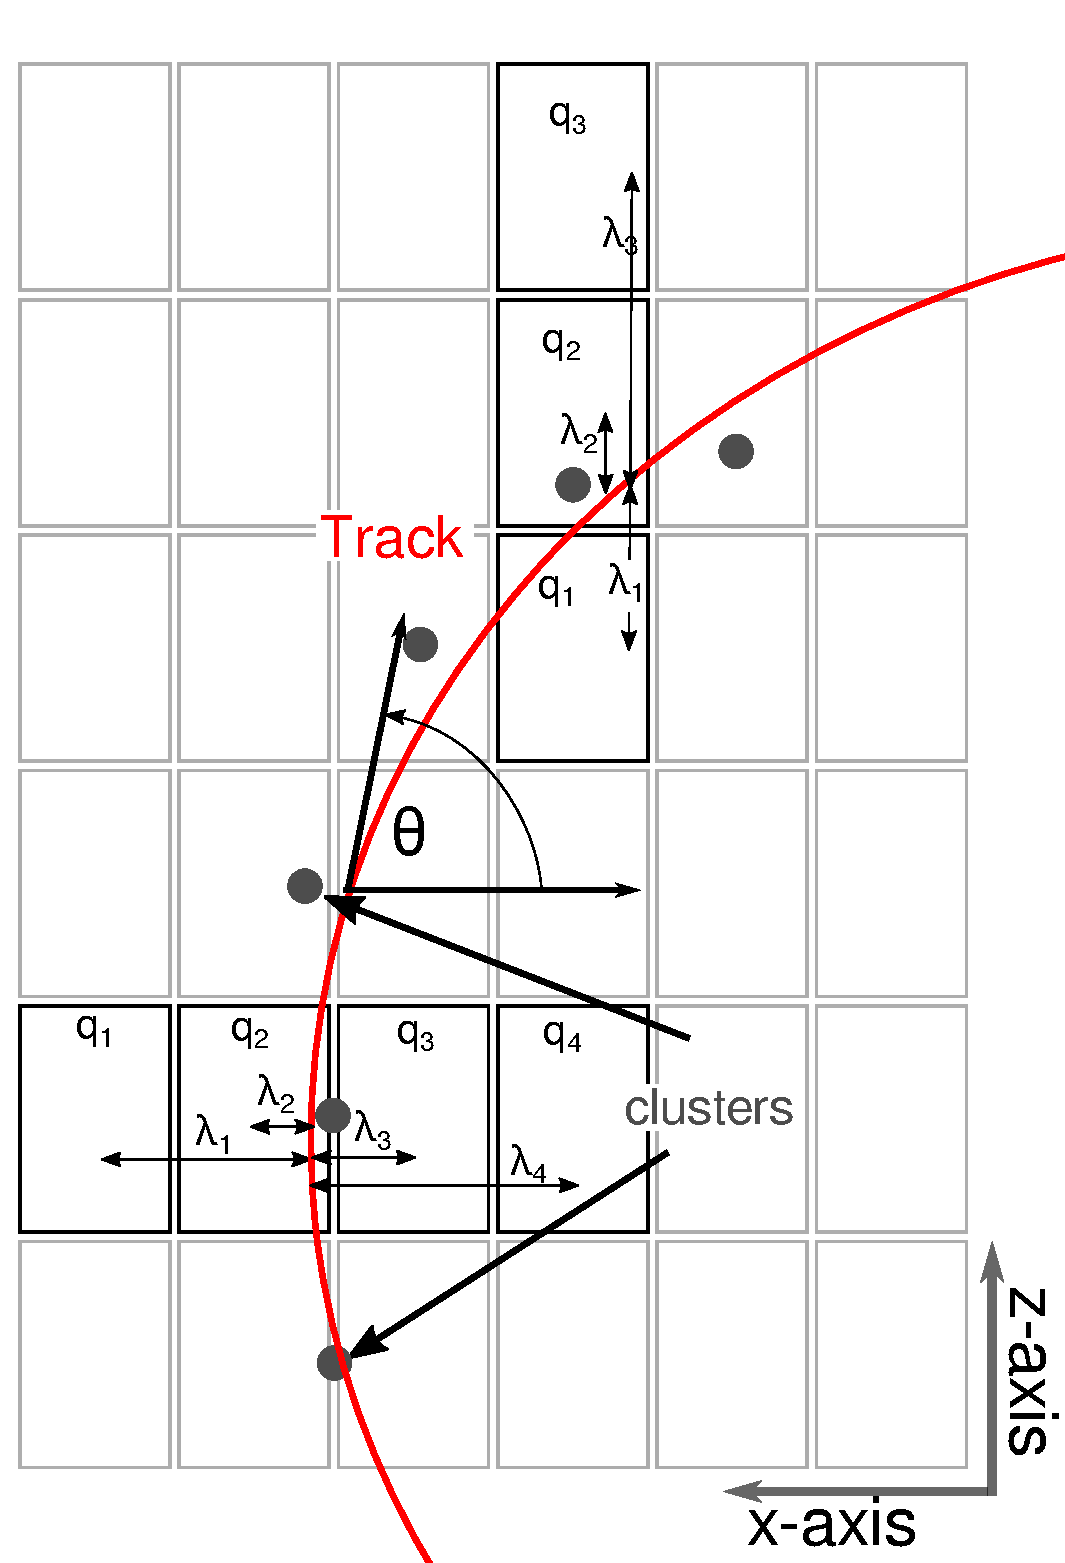
\includegraphics[scale=.5]{top_view_helix_ext.pdf}
\caption{Top down view of a fit to a track passing through several pads. Here we outline the pads in bold, where the charges $q_i$ represent the charged deposited on each pad. In this example, three clusters at the bottom are clustered in the x-direction and for the upper three clustered in the z-direction. The cluster representing each group of hits represent the average position of the track. The track fit represents the position of the avalanche, $\bar{x}$,  where the position from the center to each pad to the $\bar{x}$ position is defined as $\lambda_i$.}
\label{fig:topview}
\end{figure}

 The position along the clustering direction, $\overline{X}$, is calculated as the charge-weighted average, $\overline{X} = \sum_i q_ix_i$, where $q_i$ and $x_i$ are the charge and position of the i-th hit in the cluster. The other direction is set to the center of the pad. For example, if we are clustering hits along the x-axis, the z-position is set to the center of the pad in the z-direction and vice versa. Switching the clustering direction gives better position resolution than if we clustered only along one direction. You can imagine if we calculated the clusters only along the x-axis, tracks with $\theta \approx 0^{\circ}$ the x-position is not well defined. The cluster position and charge is stored into a new container representing the cluster called the STHitCluster class. All the clusters which belong to a particular helix track is also stored in the corresponding STHelixTrack class. 

\subsection{Correction Task}
\label{sec:corrTask}
%extend dynamic range
%PRF cut
%space charge correciton
In this task the hit distribution, within a given cluster, is checked against the measured PRF discussed in Section~\ref{sec:prf}. Figure~\ref{fig:prfpimData} shows black lines around the measured PRF in the data representing gates defining the acceptable PRF region. If the charge distribution of the hits in a particular cluster is such that less than 50\% of the hits lie within this PRF gate, the cluster is thrown out from the track. Later, in Section~\ref{sec:expPRF}, we will describe how to define the PRF for a cluster. Clusters which do not follow this PRF gate usually have been corrupted in some way. Typically this occurs when charges from other nearby tracks mix distorting the hit distribution which corrupts the energy loss and position of the cluster. This tends to occur most frequently in the dense region surrounding the target, where the track density is high. But it may occur along the track for any other reason. The width of the gate is to allow for a reasonable range of PRF values to be accepted, without biasing the data too much.   

%CONSIDER SHOWING SOME PROOF OF IT IN ACTION 

This correction task also handles several other important corrections. The first is a novel algorithm which extends the dynamic range of the electronics and is discussed in detail in Section~\ref{sec:extendDynamicRange}. The other correction task that is handled here is the space charge correction which will be discussed in more detail in Section~\ref{sec:spacecharge}. These two corrections represent the most significant corrections that greatly improve the data. 

\subsection{Momentum and track reconstruction (GENFIT)}
After all of the corrections are applied to the clusters, the cluster's position and charge values are then passed to a software package which reconstructs the momentum of the track called GENFIT. GENFIT utilizes a Kalman fitting algorithm which returns the estimated momentum and charge values for a given track \cite{genfit}. These values are then stored in into a new track container called the STRecoTrack class. 

This task is repeated a second time, but this time including the vertex as a constraining point in which all tracks are refitted. In this way, the momentum resolution is greatly improved by adding the vertex as a constraining point; since the BDC detectors, described in Section~\ref{sec:bdc}, provide very accurate x and y values for the vertex location on the target. The energy loss of the track is calculated by the truncated mean method described in Eq.~\ref{eq:truncmean}. The GENFIT task represents the final part of the analysis which pertaining to track reconstruction. From here the PID can be constructed using the energy loss, momentum, and charge information. 

\subsection{Vertex tracking (RAVE)}
\label{sec:vertex}
After all tracks are reconstructed by GENFIT, the tracks are then passed to the RAVE software package which reconstructs the event vertex from a collection of tracks \cite{rave}.  The RAVE vertex is typically referred to as the TPC vertex in this dissertation. It is used primarily to find if an event is on target by observing the z-distribution as will be discussed in Section~\ref{sec:vertexcut}. Off target events stemming from reactions in the active collimator or with the counter gas are rejected this way. After such off-target events are rejected,  we use the BDC vertex and refit the tracks as mentioned in the above section; this leads to more accurate momentum values than the TPC generated vertex provided by the RAVE routine. 



\section{Calibrations and Corrections}
In the following subsections we will discuss in detail the calibrations and corrections happening within the software framework that was outlined above.  

\subsection{Gating grid noise subtraction}
\label{sec:ggnoisesub}
Opening the gating grid is essentially done by shorting the adjacent wires in the gating grid together, and allowing them to reach equilibrium as fast as possible. Due to coupling between the gating grid, the ground plane, and other effects, the impedance of the supply cables was not perfectly matched, causing an imbalance in the current where one side discharged faster than the other side. This caused an under-damped oscillating current in the grid, which created and  oscillating residual noise early in the time bucket spectrum. Figure~\ref{fig:ggNoiseSub} shows in the upper panel shows the ADC time bucket spectrum after averaging over 2000 events in a given pad. 
 %The ground grid shielded some of the noise, but the path to ground was on two ends and was not sufficiency for this frequency.
 
\begin{figure}[!htb]
\centering
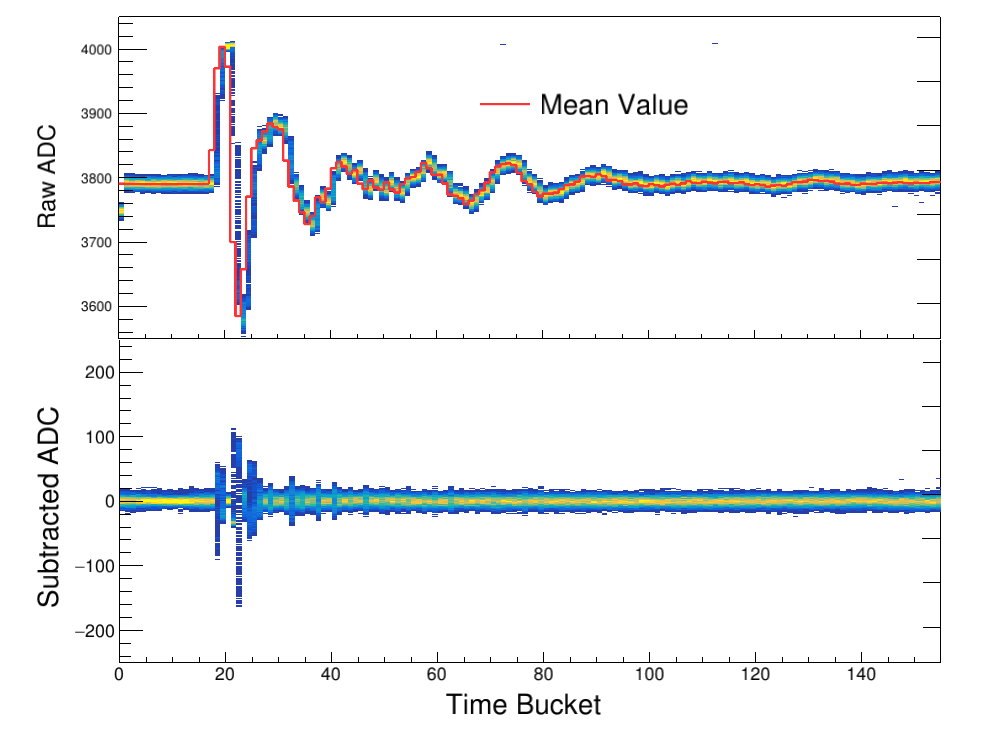
\includegraphics[width=\textwidth]{ggNoise.png}
\caption{Gating grid noise profile and subtraction for a particular pad.}
\label{fig:ggNoiseSub}
\end{figure}

The gating grid noise profile was measured by recording experimental data, only turning off the anode wires. By doing so there are no signals originating from tracks in the TPC and there is only the gating grid noise, since the grid is still being triggered. The gating grid noise was stable for a given pad and the average value --shown as the red line-- can be calculated after averaging over several thousands of events and then removed by subtracting the profile from the real data for each pad.

The bottom panel of Fig.~\ref{fig:ggNoiseSub} shows the gating grid noise self correcting itself, representing a best case scenario. The pedestal -- or base line ADC-- is around 3800 ADC in the upper panel, is automatically subtracted when subtracting the gating grid noise profile since the subtracted ADC spectra is centered around 0. Still some residual gating grid noise remains even after the subtraction, but it is significantly reduced and its extent is over a much smaller time bucket region. This failure happens in regions where the derivative of the gating grid noise is large. In these areas the ADC value is dependent upon small jitters in the timing of the signal and as a result can vary significantly from event to event. To remove this residual noise in the subtracted spectra we ignored the first 30 time buckets of the readout.

In the experiment the gating grid itself was quite stable in the  ${}^{132}$Sn and ${}^{124}$Sn systems and was not stable in the ${}^{108}$Sn and ${}^{112}$Sn beams, where gating grid resistors broke in these earlier runs many times. Because of this, the gating grid noise was monitored regularly and we took gating grid noise profiles frequently, especially after a gating grid board was replaced. 


%The average noise profile was constructed by averaging all the events in the gating grid runs, pad-by-pad; each pad had a slightly different noise profile since the impedance to each pad was slightly different. It is worth noting that the small electronics noise would be effectively canceled out by averaging over thousands of events. During the first stages of the software, the gating grid noise profile closest to that run would be subtracted from the raw data canceling the gating grid noise in that run. 

\subsection{Cocktail calibration}
\label{sec:cocktail}

\begin{table*}\centering
\ra{1.3}
\begin{tabular}{@{}rrrrrrr@{}}\toprule
& \multicolumn{3}{c}{$100 MeV Target$}\\
\cmidrule{2-4}
Particle &\phantom{abc} & Measured & Corrected & \% Difference Raw & \% Difference Corrected\\
\midrule
p   & 882.8 & 929.5 & 877.3   &  3.7  & -1.0  \\
d   & 817.1 & 831.15 & 797.94 &  1.7  & -2.3\\
\bottomrule
\end{tabular}
\caption{Summary of expected cocktail for the calibration run taken with the Al target. }
\label{tb:cocktail100tar}
\end{table*}

\begin{table*}\centering
\ra{1.3}
\begin{tabular}{@{}rrrrrrr@{}}\toprule
& \multicolumn{3}{c}{$100 MeV$}\\
\cmidrule{2-4}
Particle & Expected & Measured & Corrected & \% Difference Raw & \% Difference Corrected\\
\midrule
p   & 882.8 & 903.5 & 889.0 &  2.0   & -1.6  \\
d   & 817.1 & 898.5 & 874.5 &  2.1   & -2.7\\
\bottomrule
\end{tabular}
\caption{Summary of expected cocktail from the lower beam energy.}
\label{tb:cocktail100}
\end{table*}

\begin{table*}\centering
\ra{1.3}
\begin{tabular}{@{}rrrrrrr@{}}\toprule
& \multicolumn{3}{c}{$300 MeV$}\\
\cmidrule{2-4}
Particle & Expected & Measured & Corrected & \% Difference Raw & \% Difference Corrected\\
\midrule
d   & 1621 & 1704 & 1612   &  5.1 & -0.6  \\
t   & 1612 & 1691 & 1596   &  4.9  & -1.0\\
${}^{4}$He   & 1613 & 1698 &  1595 & 5.3 & -1.1\\

\bottomrule
\end{tabular}
\caption{Summary of expected cocktail from the higher beam energy.}
\label{tb:cocktail300}
\end{table*}

A cocktail of several light charged particles (p,d,t,${}^{3}$He,${}^{4}$He) of well defined magnetic rigidity was produced was produced and measured in the TPC to provide a momentum calibration of the TPC. The magnetic and slit settings of the dipoles in the BigRIPS spectrometer were set so that the momentum resolution of the beam was defined to better than $\delta p/p$ < 1\%. Two magnetic rigidity settings were studied with no target in place. A thick Aluminum target was also inserted to provide a slightly lower energy calibration point for part of the lower rigidity setting, effectively creating three energy calibration points over several particle species. In some cases the certain particles were not able to propagate or were strongly attenuated and resulted in measurements of poor statistical precision. 

Since the cocktail beam was a mono-energetic source of particles and rigidity selection in the BigRIPS corresponding to an actual momentum resolution of better than 1\%, we can interpret the  observed momentum resolution as a measurement of the intrinsic TPC momentum resolution of the TPC for these particles. The momentum resolution in general depends on several factors such as the particle's angle, momentum, charge, track multiplicity, etc. This calibration beam represents an ideal situation where the track was parallel to the pad plane and the track is not affected by the presence of other tracks. The average momentum resolution was measured to be $dp/p = 2\%$ over the full range of particle species for all settings as measured by the sigma of the Gaussian momentum distribution. 

The energy loss resolution can also be directly measured from the monochromatic source provided by the cocktail beam. Each particle species in the cocktail beam has a well defined most probable energy loss;  the energy loss resolution was measured to be approximately 5\% for all particles. These measurements are summarized in Table~\ref{tb:momresolution}.

Since the magnetic dipole setting of the BigRIPS spectrometer is well defined, we can calculate the expected momenta of each particle species measured. The energy losses through various materials in the beam line were propagated using LISE++ software \cite{lise++}. We found that the momenta of light particles in the  cocktail calibration beam differed significantly (up to 5\% ) from the expected values. This is shown in Tables~cref{tb:cocktail100tar,tb:cocktail100,tb:cocktail300}. We could address this discrepancy by incorporating the smaller horizontal magnetic field components at the edge of the dipole and taking into account the electron drift velocities in the direction of $\vec{E}\times\vec{B}$ direction as seen from Eq.\ref{eq:elecdrift}. The $\vec{E}\times\vec{B}$ drift velocity causes the electron trajectories to shift toward the +x-axis in the TPC coordinates causing particles of positive charge (going in the -x-axis) to have a higher measured momenta than in reality.  The details of the correcting for the $\vec{E}\times\vec{B}$ effect will be discussed later in Section~\ref{sec:spacecharge} in a more general way which also includes the correction for the presence of positive space charge in the field cage volume. The same correction technique was applied here, where the cocktail beam is the special case of zero space charge.

(Tables~\cref{tb:cocktail100tar,tb:cocktail100}), protons see a slight improvement of about ~1\% where as the deuterons are over corrected in both settings. In general, all these light particles corrected momentum are of the order of 1\% smaller than value given by the rigidity selection in the BigRIPS separator. This discrepancy could reflect the accuracy of our knowledge of the magnetic field of the SAMURAI dipole. Without a definitive explanation for this discrepancy, we have not attempted further correction of the calculated momenta. We note that it is of the same order as the resolution of the measurement of these momenta.  

\begin{table*}\centering
\ra{1.3}
\begin{tabular}{@{}cc@{}}\toprule
Momentum Resolution \% & <dE/dx> Resolution \% \\
\midrule
1.6  & 4.6\\
\bottomrule
\end{tabular}
\caption{Summary of the estimated momentum and energy loss resolutions.}
\label{tb:momresolution}
\end{table*}

%Apendix of the beam line elements
%apendix of the settings of the bigrips elments
%Picture of cocktail before and after ExB effect
%Table of LISE++ expected cocktail energies ridigity setting of dipole magnets (reference big rips line)


\subsection{Electronics calibration}
\label{sec:elecCalib}

\begin{figure}[!htb]
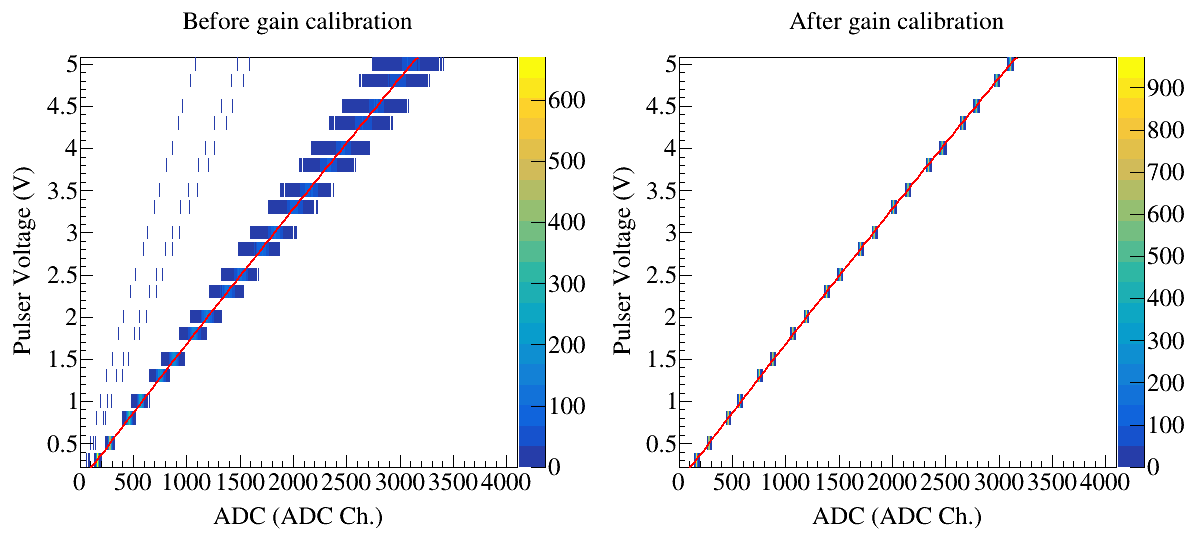
\includegraphics[width=\linewidth]{gaincalib.png}
\caption{Repose of each channel in the electronics to various input voltages of an input signal supplied by a pulse generator.}
\label{fig:gaincalib}
\end{figure}

The electronics were calibrated by measuring the response of each channel to an input signal supplied by a pulse generator. This is a relative calibration technique with the intent to calibrate the varying gains in each channel relative to one another, not an absolute calibration. The pulse was distributed to all the electronics channels by pulsing the ground plane for a range of input voltages. This distributed the pulse evenly across the entire pad plane. The input voltage is plotted as a function of the measured height of the pulse in the electronics channel given in units of ADC in Fig.~\ref{fig:gaincalib}, for every channel. The small variation in each channel can be seen as the wide band around each measurement point. A linear fit is performed to get the calibration line for each channel. A particular channel is chosen which provides a reference calibration to which the slopes of all other channels are calibrated too.   The right panel shows the resulting distribution of channels after calibration, in which the channel variation is reduced significantly. 



\subsection{Anode gain calibration}
\label{sec:anodeCalib}
As discussed in Section~\ref{sec:wireplanes} the voltage of the anode sections 12 and 14 were reduced during the experiment due to high currents being observed on the wires due to a leak in the gating grid that has since been corrected. Out of all the runs used in the analysis in this thesis -- see \ref{tb:runList} -- the anode sections 12 and 14 were lowered to \SI{1085}{\volt} for runs 2272-2371 and set to \SI{1214}{\volt} for all other runs. By lowering the voltage on these anode wires, the gas gain is lowered as compared with all the other anode wire plane sections which operate at \SI{1460}{\volt}. To account for the drop in gain, we artificially increase the gain of the pads which lie above these anode wires in the software. The multiplicative factor is estimated by plotting the energy loss in the high gain sections relative to the low gain sections.



\begin{figure}[!htb]
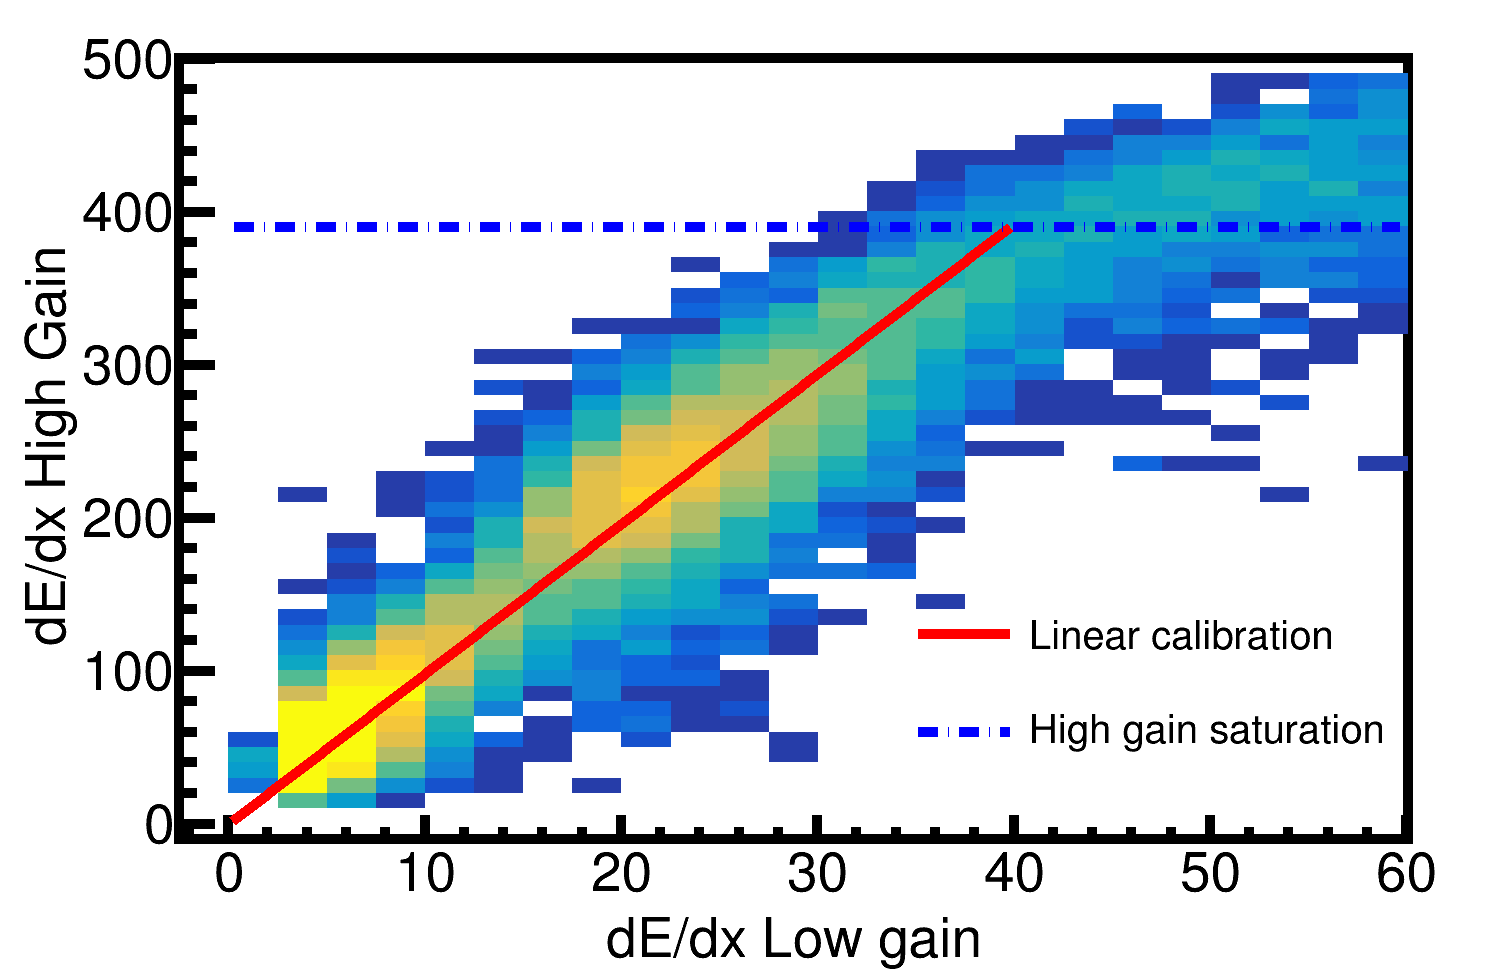
\includegraphics[width=\linewidth]{highlowcal.png}
\caption{Calibration of low and high gain sections of the anode wires.}
\label{fig:highlowcal}
\end{figure}

Figure~\ref{fig:highlowcal} shows the correlation plot of $\langle dE/dx\angle$ of the high versus the low gain sections. The effects of the high gain channel saturation can around a value of 400 ADC\si{\per\milli\metre} and plateaus, where as the low gain does not; this region is left out of the fit. A linear fit was performed for the calibration between the high gain channel $h_c = G\cdot l_c$, where $l_c$ is the value of the low gain channel and $G$ is the gain factor. In the case where the low anode voltage was \SI{1214}{\volt}, the $G=9.8$, where in the case of \SI{1085}{\volt}, the $G = $.  

 A map defining the gain calibration of each pad is pre-loaded into the software. In the decoder task the raw ADC spectra was multiplied by this gain factor for each channel. The PSA thresholds of those channels also were multiplied by the same gain factor since the noise levels were also artificially magnified as well. 

\subsection{Extending the dynamic range of the Electronics}
\label{sec:extendDynamicRange}

Using a TPC for measurements of HICs in intermediate energy heavy ion collisions presents a different set of challenges as opposed to higher energy experiments. Typically in higher energy experiments fundamental particles are produced with charge $\pm e$. Also, the particles are traveling at higher energies in which the energy losses are near or close to the minimum ionization in the energy loss. In these cases the dynamic range of most TPC electronics can cover a wide range of particles. In nuclear HICs, we are interested in measured particles with charges $Ze$ where Z=1-3, and even higher in some applications. Since the energy loss in the Bethe-Bloch equation, Eq.~\ref{eq:bb}, is proportional to $Z^2$, the range of energy losses reflects the possible range of z values. Even more, in low energy nuclear HIC of intermediate beam energies -- around \SI{300}{\MeVA} -- produce low velocity particles which exist in the $1/\beta^2$ region of Eq.~\ref{eq:bb}, where the energy loss grows dramatically. In this case, the limited dynamic range of electronics significantly limit the PID as the charge of a particle increases and the velocity decreases, leading to very large and even saturated pulses in the electronics. 

Several TPCs have tried to address this issue by having regions of low and high gain, either in amplification gain or in electronics gain. This mitigates the complete loss of information but introduces a new problem. Particles which deposit large amounts of charge will have good measurements in the low gain areas, whereas particles depositing minimal energy losses will lose information in the same low gain areas. The reconstruction of such tracks will suffer. There are ongoing efforts in the nuclear community to develop new electronics which hope to mitigate these issues by developing more sophisticated  pre-amplifiers and electronics \cite{feanics,feanics2}.  Never the less, it is useful to develop a software technique which extends the dynamic range of TPC electronics without the use of new external hardware. Which can be particularly useful for experiments which have already taken data with older electronics technologies. In this section we will outline a novel software technique that takes advantage of the PRF described in Section~\ref{sec:prf} and can effectively extend the dynamic range of the TPC electronics. 

In TPCs, the effective dynamic range is very different from the single channel dynamic range depending on how the TPC measurement is used. Typically TPCs are operated inside of a magnetic field for the purpose of reconstructing the momentum of a track, which requires sub-millimeter precision in the position determination along the track path. This is achieved by clustering several pads together as discussed in Section~\ref{sec:helixtrack}. To achieve this at least 2 adjacent pads must be measured, and the precision increases as the number of adjacent pads increases. 

In this case the effective dynamic range is not the single channel dynamic range, but the relative dynamic range between central pad --holding the largest charge-- and the adjacent pads --holding the smaller charges in the PRF distribution. For example, to measure minimum ionizing particles, the Signal-to-Noise-Ratio (SNR) of the pad with the smallest charge in the distribution should be some reasonable value above noise, so that the full charge distribution can be measured. From the PRF in Section~\ref{sec:prf}, we know the central pad in the cluster holds about 80\% of the total charge, where as the two adjacent pads each hold the remaining 10\%. In the \spirit TPC the electronics gain was set so that the the pads have a SNR of 6:1 for minimum ionizing tracks, and therefore the central pad had a SNR of 50:1. The maximum SNR in the central pad -- before the electronics saturate -- the SNR is 800:1. Therefore the maximum SNR is roughly 16 times larger than that of minimum ionizing particles. 

Figure~\ref{fig:intro} shows the theoretical energy loss curves for several particles as a function of rigidity $p/q$. Minimum ionization can be seen to take place around \SI{10}{\kilo\electronvolt\per\centi\metre}. The dashed lines and vertical blue bar in are separated by a factor of 16, representing the effective dynamic range in the \spirit TPC. This dynamic range should be regarded as approximate because the energy loss fluctuates significantly about the most probable energy loss as described in Section~\ref{sec:energyloss}. Nevertheless, the blue dashed lines and vertical blue bar illustrate that the range of energy losses sampled in a fixed gain readout system is limited. One can change the gain and shift the energy loss range that can be sampled, but the dynamic range itself cannot be increased.

  
\begin{figure}[ht!]
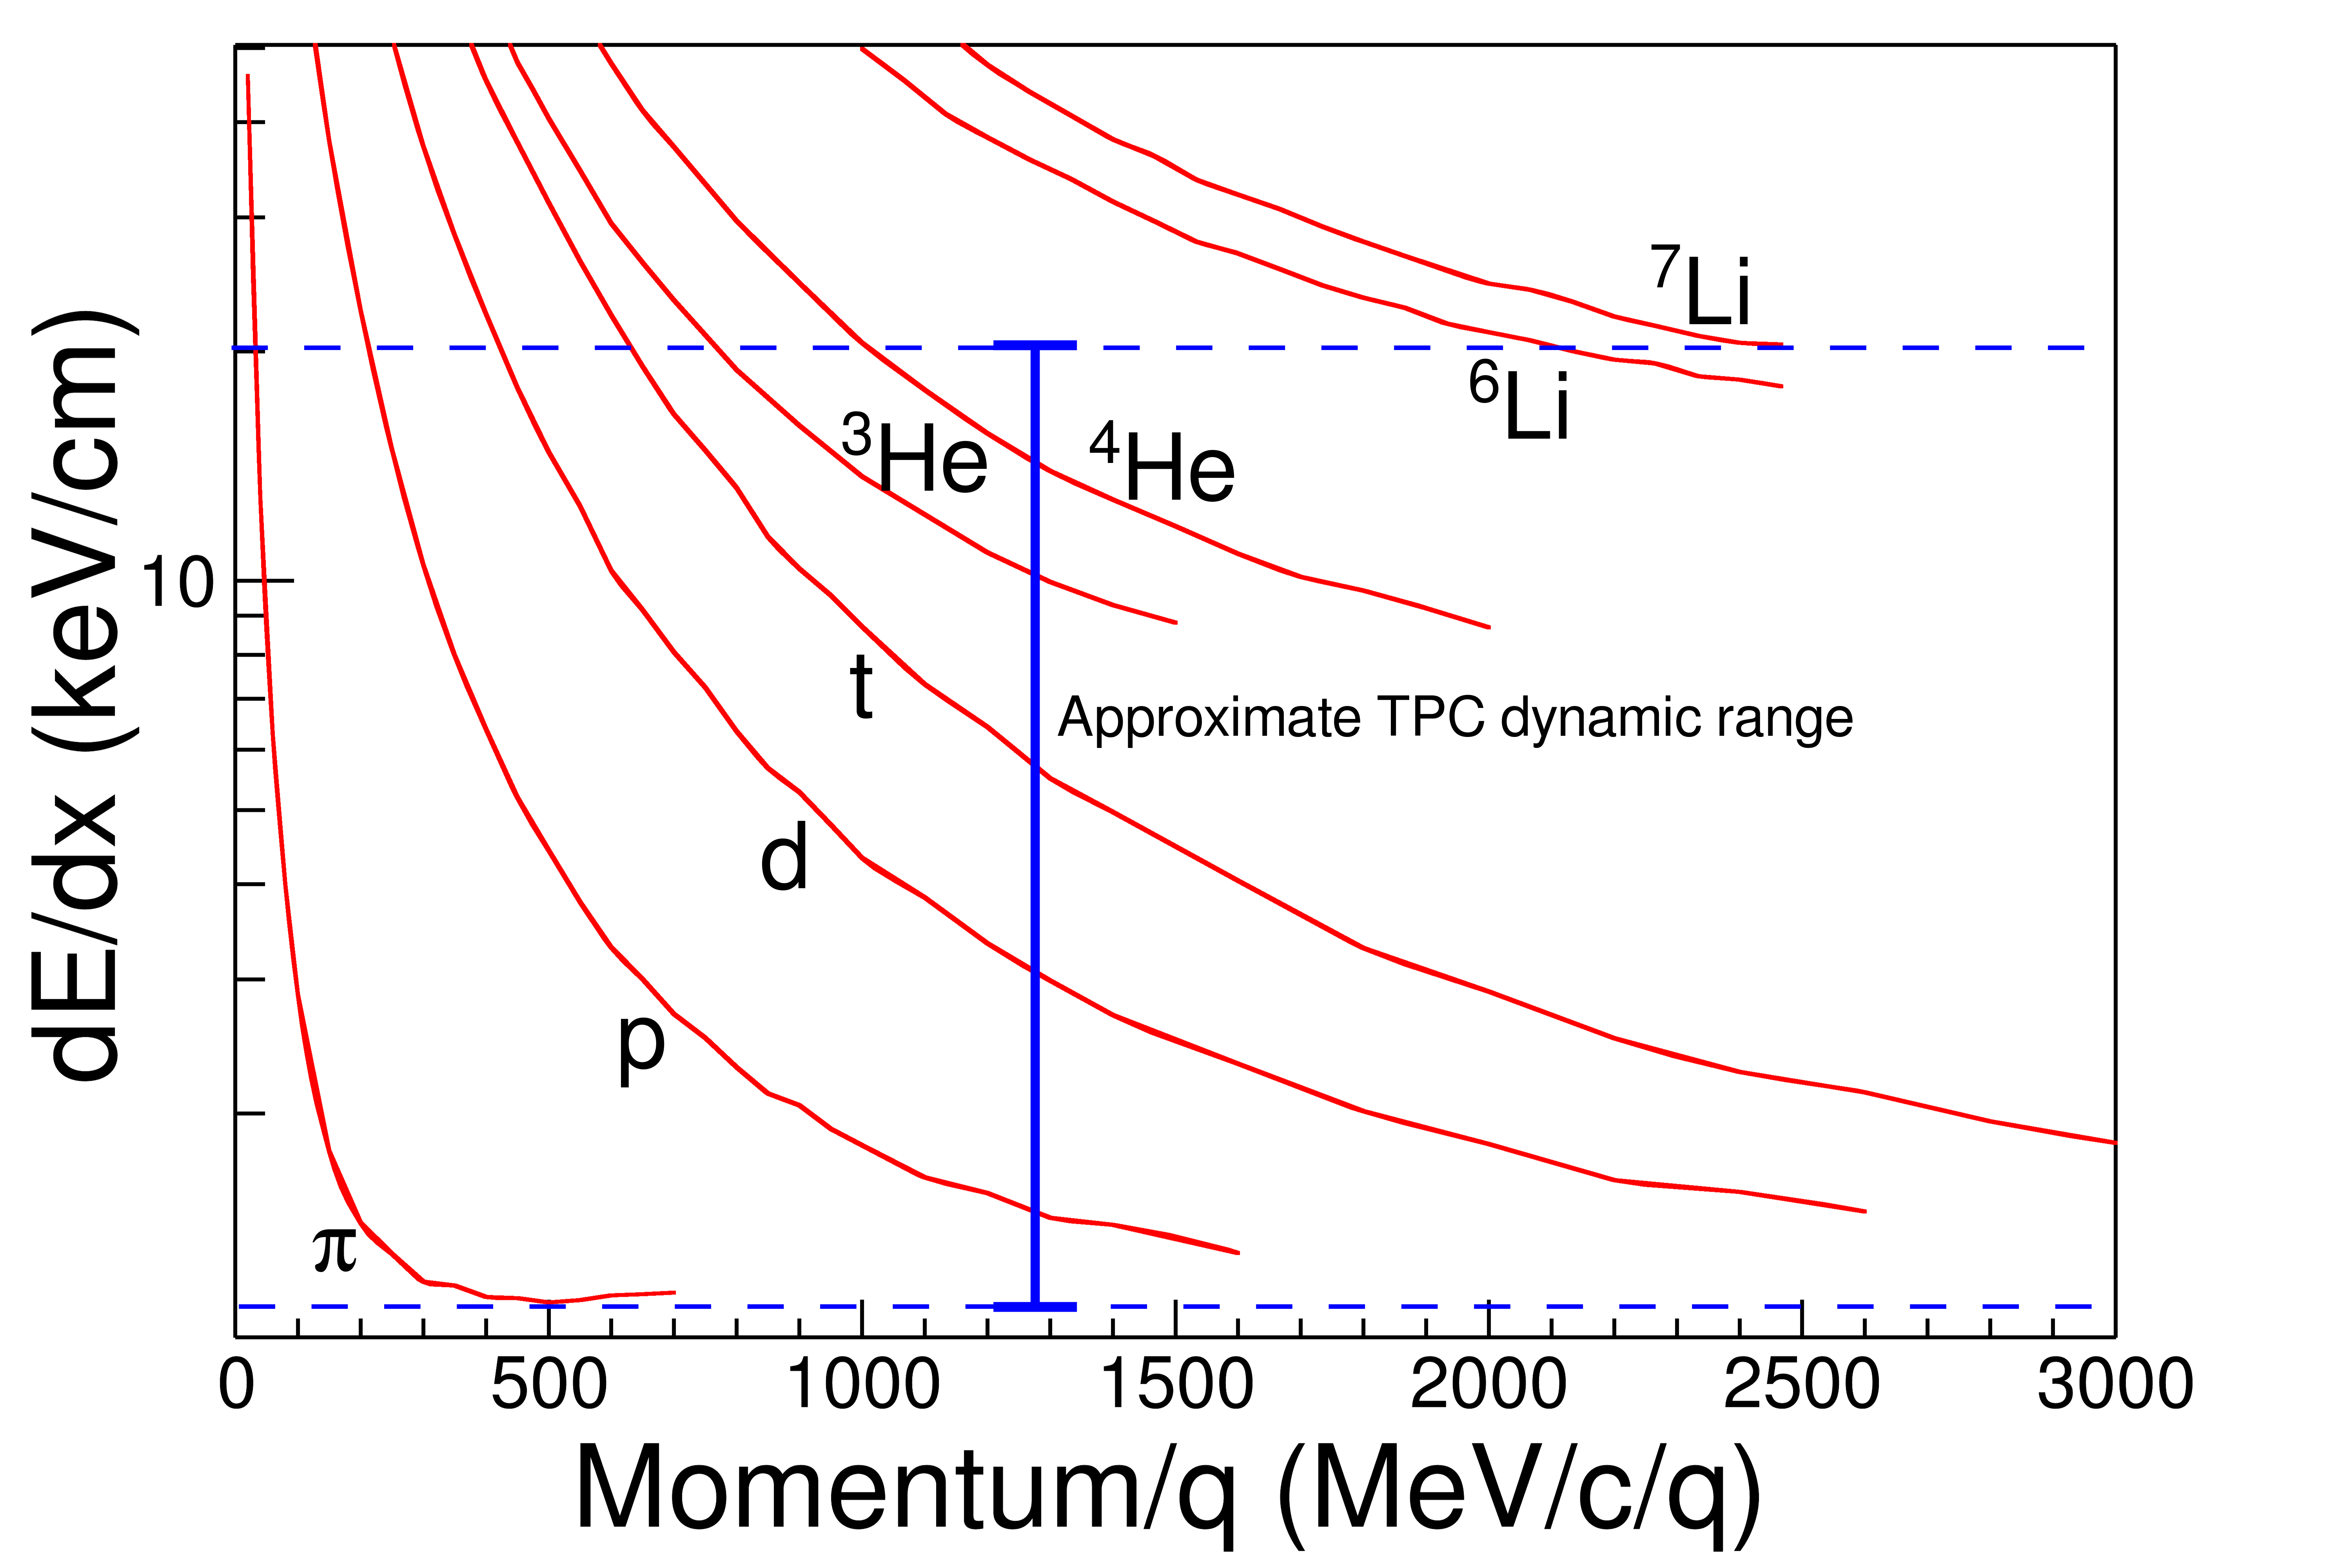
\includegraphics[width=\linewidth]{intrographic}
%\includegraphics[width=\linewidth]{intrographic_2}
\caption{The expected $dE/dx$ lines of different particles are given in red as calculated by Geant4. The approximate dynamic range of the TPC is shown by the vertical bar for the gain setting used in the experiment. Anything outside of this region would be saturated to some degree.}
\label{fig:intro}
\end{figure}


\subsection{Experimental Pad Response Function}
\label{sec:expPRF}
As mentioned in Section~\ref{sec:prf}, the PRF depends on the angle of the track as it crosses the wires and pads. The PRF of the TPC was experimentally determined from non-saturating hits and clusters in tracks at various track crossing angles. As in Fig.~\ref{fig:topview}, we postulate that the PRF is a function of the total charge deposited in a cluster $Q = \sum_i q_i$, and the difference in position of the center of the $i^{th}$ pad, $x_i$, to the mean position $\bar{x} = \sum_i x_i q_i/Q$, defined as,

\begin{equation}
\lambda_i = x_i-\bar{x}. 
\label{eq:lambda}
\end{equation}

The PRF is simply defined as the charge fraction of each pad as a function of $\lambda$, as shown in Equation \ref{eq:prf}. 

\begin{equation}\label{eq:prf}
PRF(\lambda_i) = \frac{q_i(\lambda_i)}{Q}
\end{equation}

Averaging over many events in the experimental data, the resulting PRF is particularly well behaved for the S$\pi$RIT TPC as seen in Fig.~\ref{fig:expprf}. Here we see the deviations from the expected analytic Gatti distribution (black curve). Fitting with a two parameter Gaussian function -- the red curve -- describes the data better. The PRF was fit with a two parameters Gaussian function, where $N_)$ is the normalization coefficient and $\sigma$ the corresponding width:

\begin{equation}\label{eq:gaus}
PRF_{\mathrm{Gaus}}(\lambda) = N_0 e^\frac{-\lambda^2}{2\sigma^2}.
\end{equation}


\begin{figure}[ht!]s
\begin{overpic}[width=\linewidth]{fig5.pdf}
\put(61,55){\contour{white}{ PRF${}_{\mathrm{Gaus}}(\lambda)$ eq. \ref{eq:gaus}  }}
\put(61,49){\contour{white}{ PRF${}_{\mathrm{Gatti}}(\lambda)$ eq. \ref{eq:gatti} }}
\end{overpic}
\caption{Experimental pad response function of many events for a crossing angle of $85^{\circ} < \theta \leq 90^{\circ}$.  }
\label{fig:expprf}
\end{figure}



The shape of the PRF depends on the crossing angle of the track, which determines how wide the charge is distributed along the wire \cite{gatti}. Figure~\ref{fig:prfpimData} shows the PRF for $\pi^-$ tracks versus the crossing angle $\theta$ of the track. The PRF gets wider starting from $90^{\circ}$  until where the clustering switches directions at $\ang{45}$. If we did not switch clustering directions the PRF would become wider until it was a uniform distribution and there was no position resolution. Switching shows the opposite trend where the PRF becomes narrower going from $45^{\circ}$ to $0^{\circ}$, as the position resolution gets better.

\begin{figure}[!htb]
     \centering
	 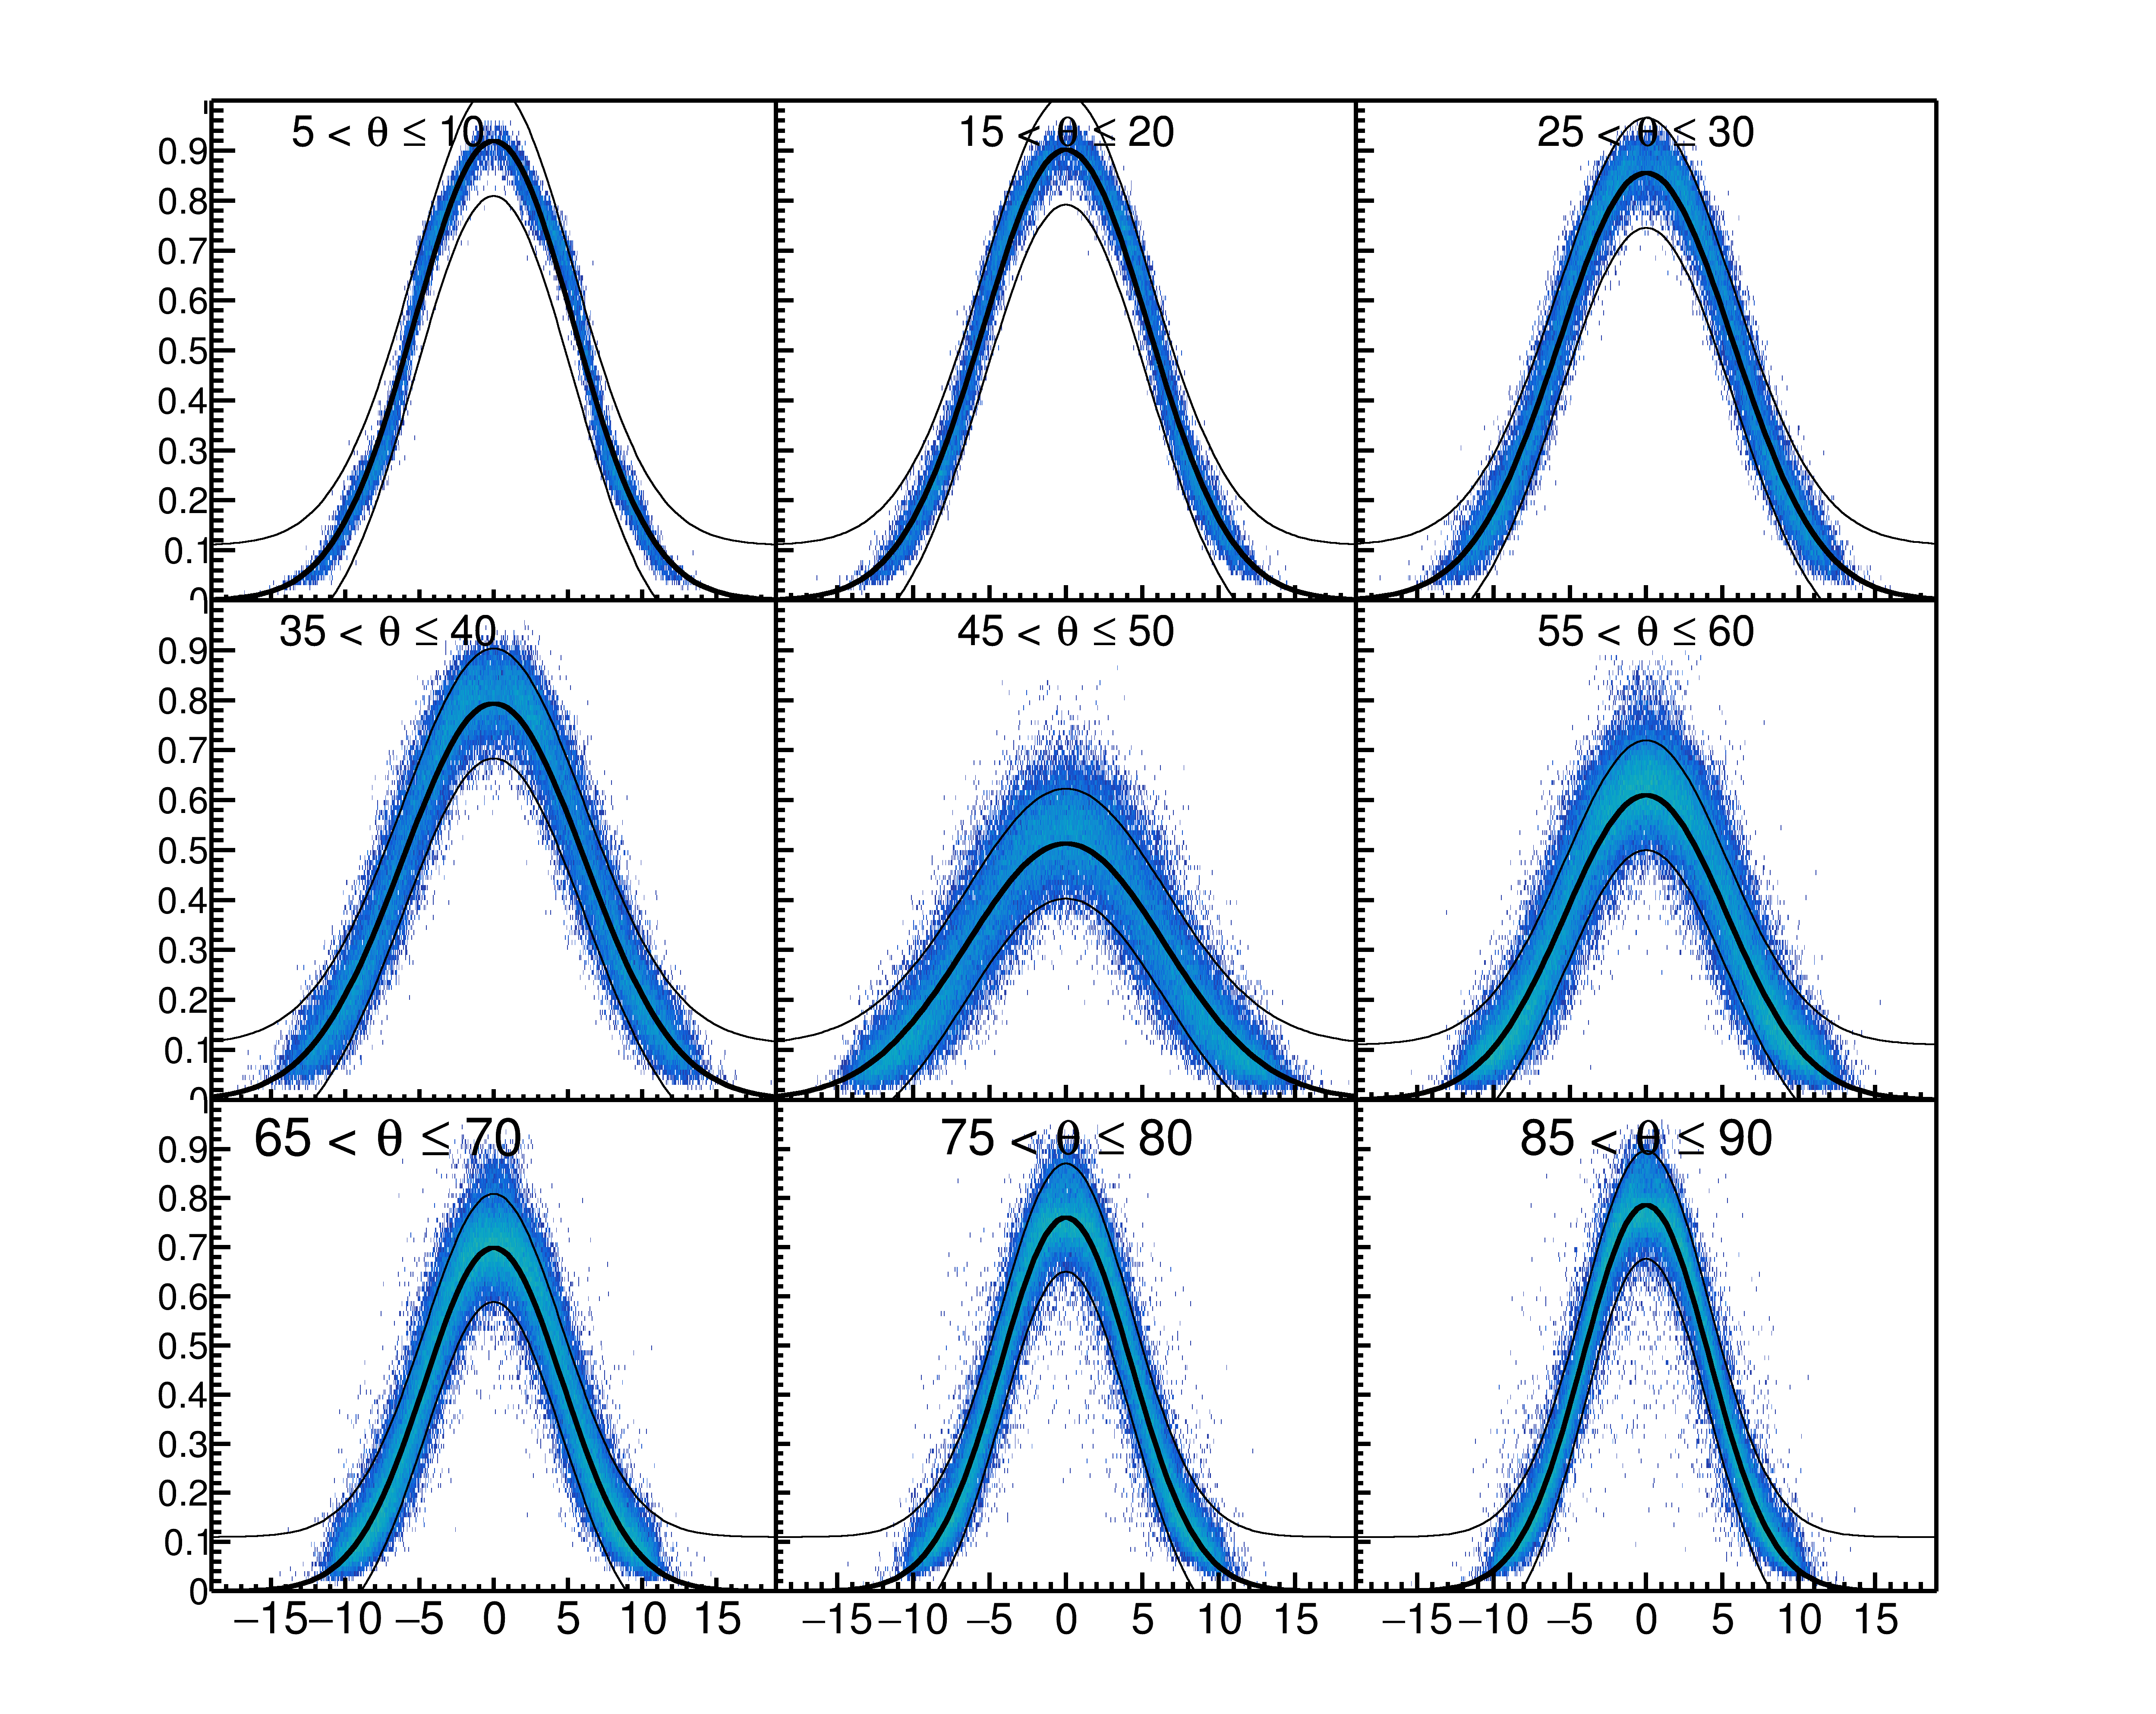
\includegraphics[width=\textwidth]{PRFs_data_wcut.png}
     \caption{Pad Response Function of $\pi^-$ tracks in experimental data. }
     \label{fig:prfpimData}
\end{figure}

\begin{figure}[ht!]
\vspace{5mm}
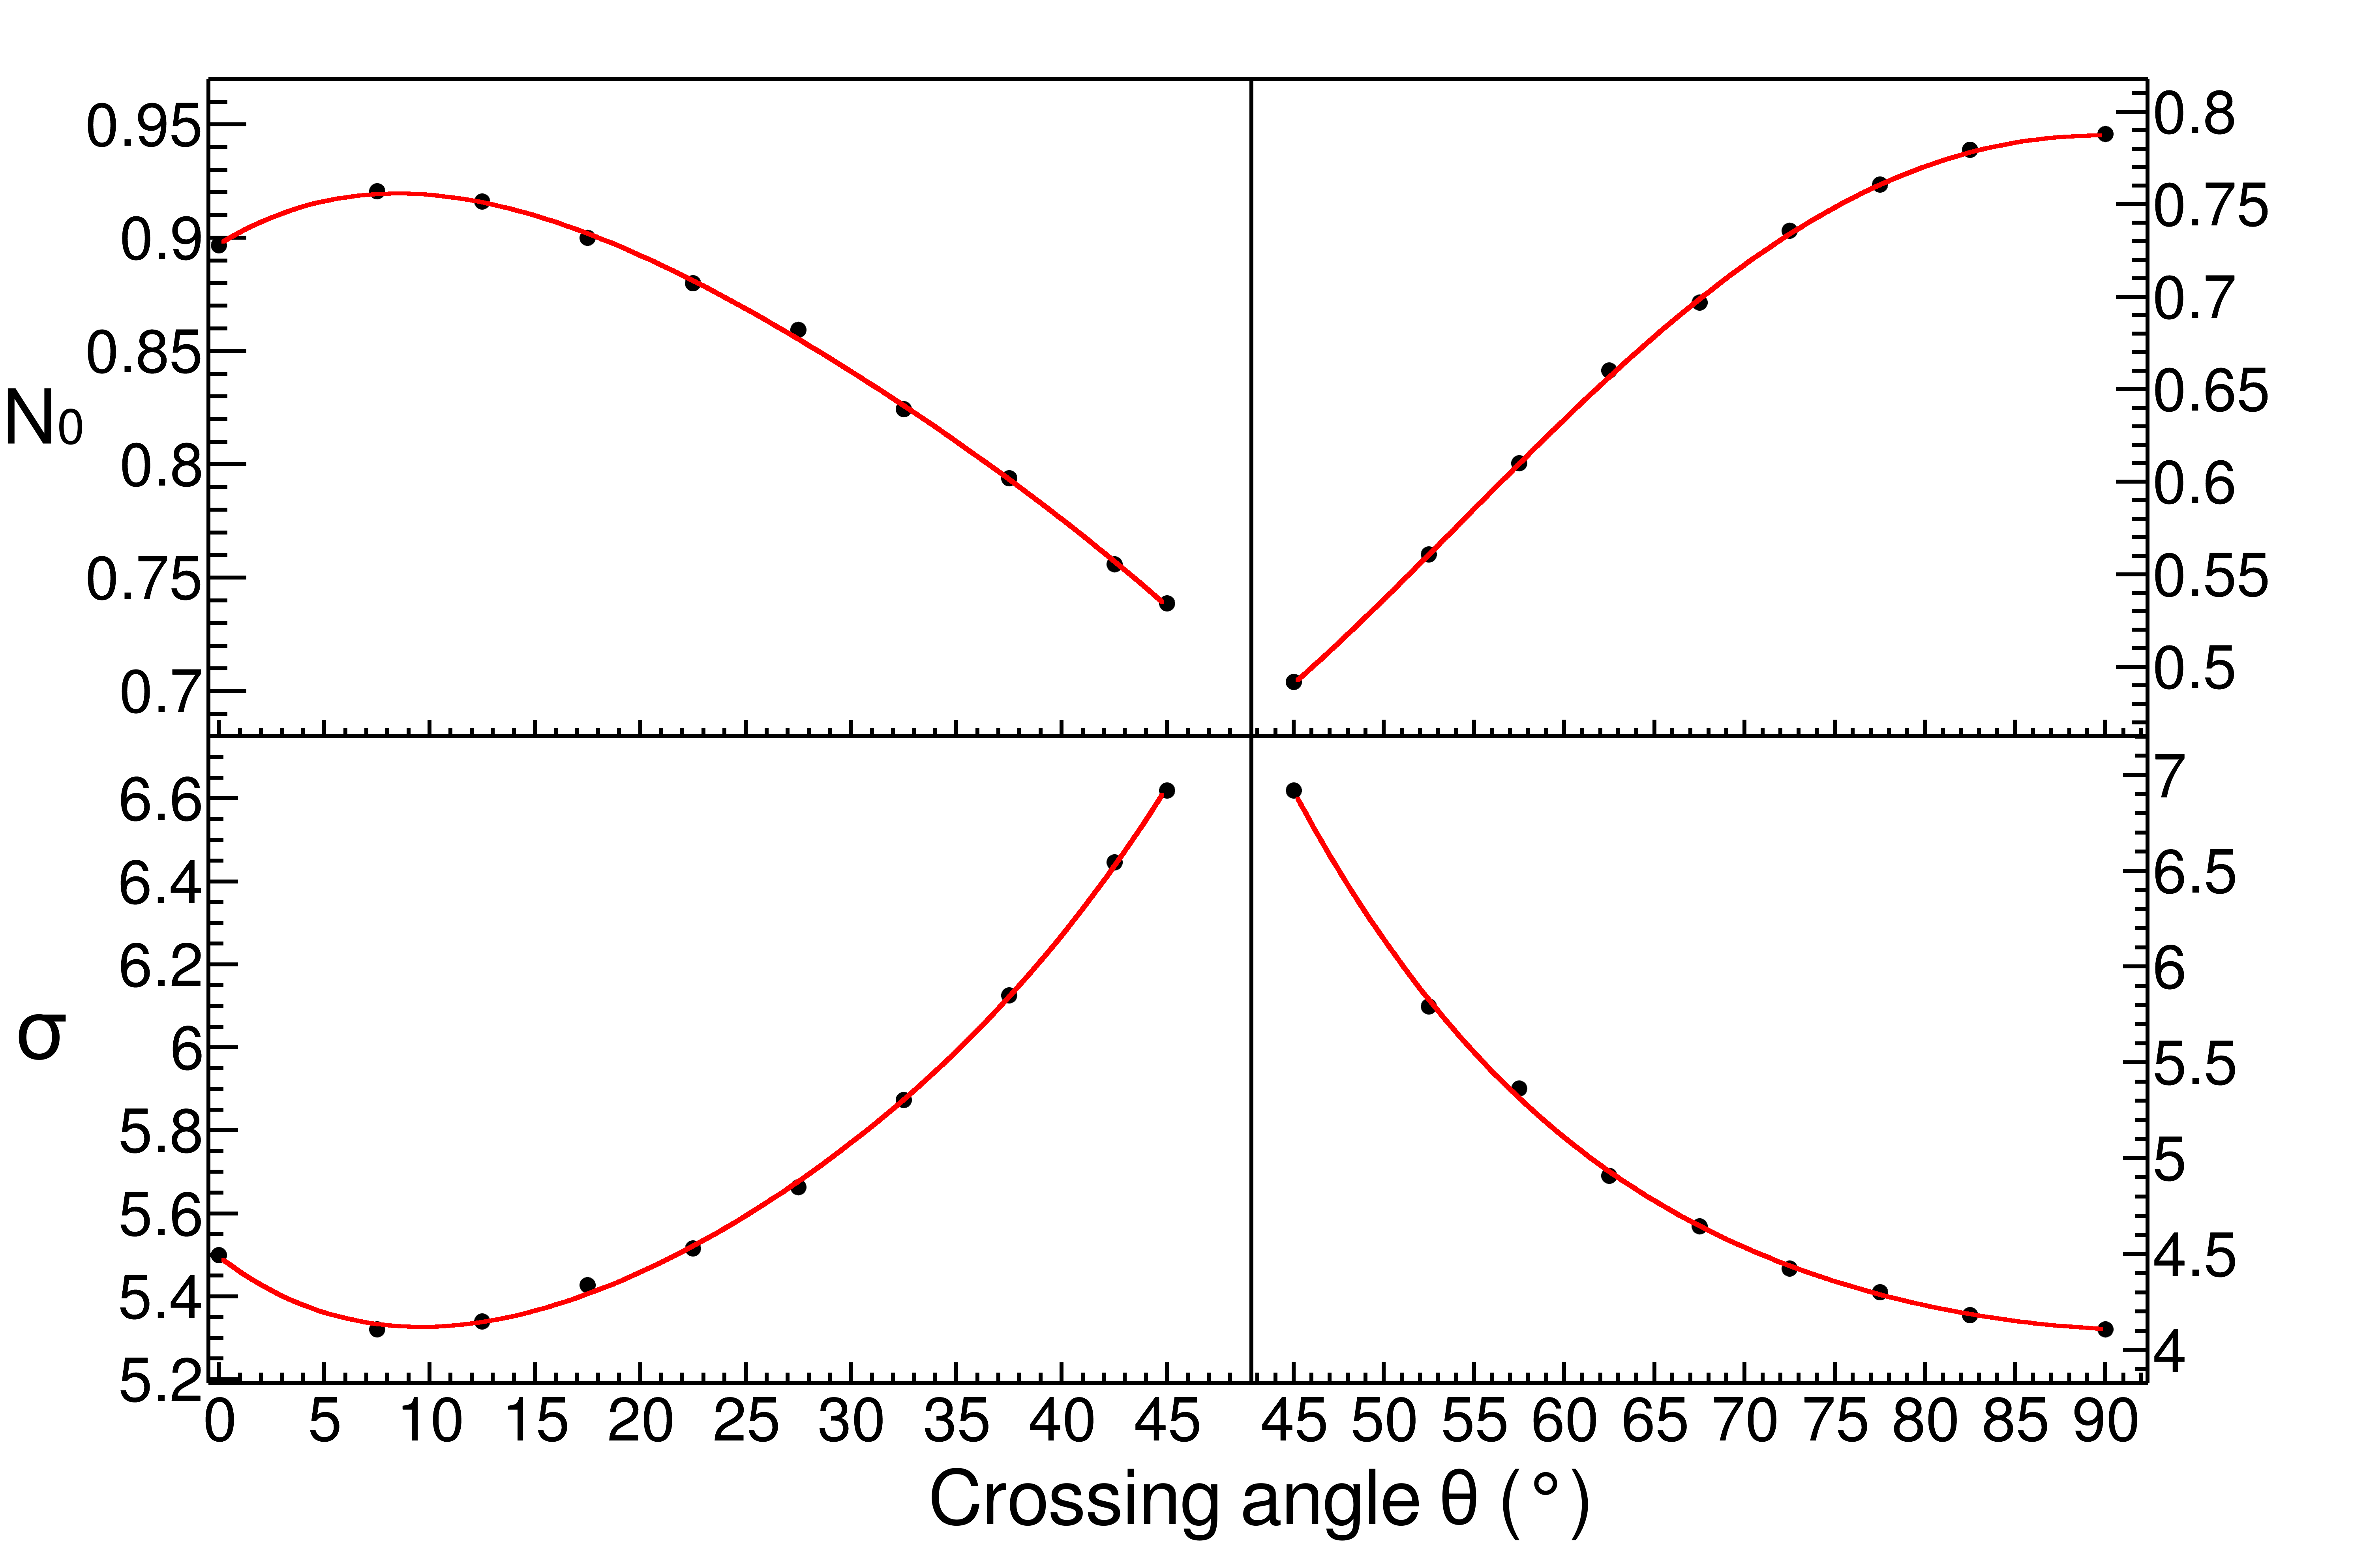
\includegraphics[width=\linewidth]{fig7}
\caption{Parameters $N_{0}$ and $\sigma$ as a function of the crossing angle $\theta$ with the $4^{th}$ order polynomial fits.}
\label{fig:normsigma}
\end{figure}

\begin{comment}
\begin{table}
\centering
 \begin{tabular}{||c c c c c c||} 
 \hline
 Coefficient & $c_0$ & $c_1$ & $c_2$ & $c_3$ & $c_4$ \\ [0.5ex] 
 \hline\hline
 $0 < \theta < 45$ & & & & &  \\ [.25ex]
 \hline
 $N_0$ & .897 & 5.766E-3 & -4.263E-4 & 7.444E-6 & 5.705E-8 \\ 
 \hline
 $\sigma$ & 5.496 & -3.920E-2 & 2.693E-3 & -5.208E-5 & 5.334E-7\\
 \hline
 $45 < \theta < 90$ & & & &  & \\ [.25ex]
 \hline	
 $N_0$ & 1.220 & -6.258E-2 & 1.608E-3 & -1.492E-5  & 4.654E-8 \\
 \hline
 $\sigma$ & 31.368 & -1.109 & 1.779E-2 & -1.336E-4 & 3.940E-7\\
 \hline
\end{tabular}
\caption{Coefficients of the $4_th$ order polynomial fit to the Gaussian parameters $N_0$ and $\sigma$. The polynomial form is given as $c_0 + c_1 x + c_2 x^2 + c_3 x^3 + c_4 x^4$}
\label{tb:coeff}
\end{table}
\end{comment}
 
The Gaussian fit was performed on each PRF for a crossing angle steps of  $\ang{5}$ ranging from $\ang{0} < \theta \leq \ang{90}$. Figure~\ref{fig:normsigma} shows the two parameters resulting from fitting the the Gaussian function -- Eq.~\ref{eq:prfgaus} -- which are are plotted versus $\theta$. A $4^{th}$ order polynomial fit of these parameters allowed for interpolating for any given $\theta$ value, which is shown as the black line. Once we have this interpolation, we can predict the PRF for any given value of $\theta$. 


\subsection{Method of Desaturation}
\label{sec:desat}

\begin{figure}[ht!]
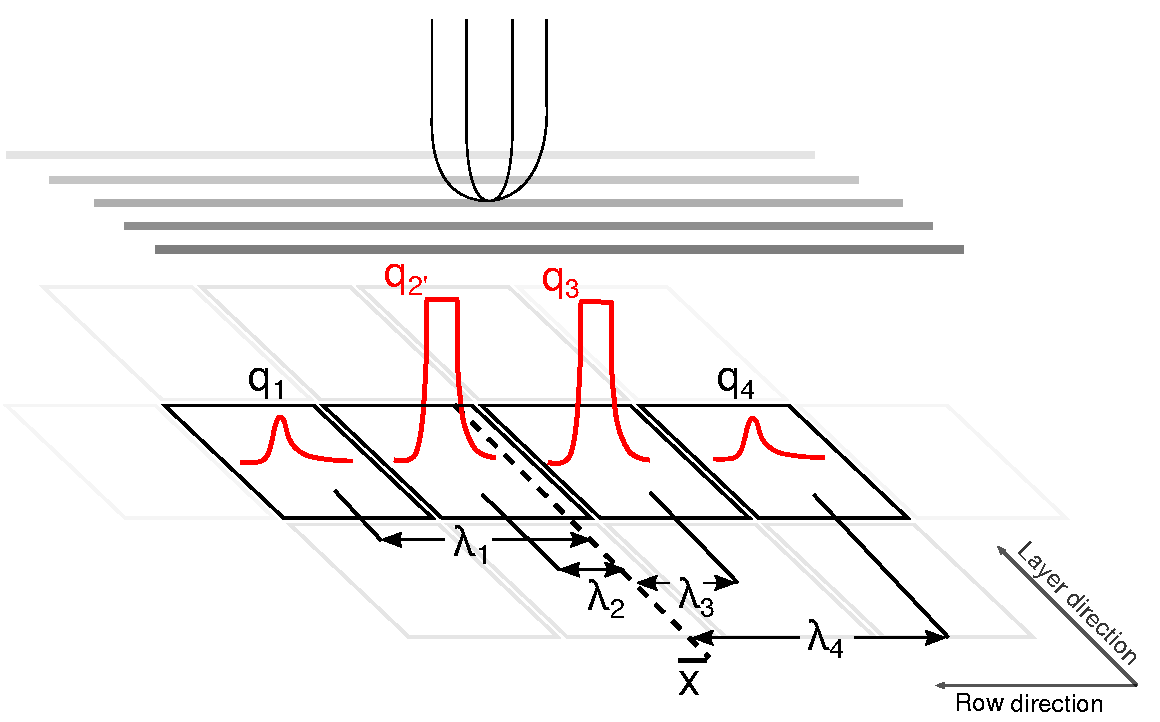
\includegraphics[width=\linewidth]{saturated_pads}
\caption{A typical case of a saturating event. The red pulses represent the time bucket signal for each collected charge. The pads directly underneath the avalanche point, $q_{2'}$ and $q_{3'}$, are saturated while pads farther away, $q_1$ and $q_4$ are not saturated.}
\label{fig:satpad}
\end{figure}

In the following, we will use the term \emph{desaturation} to describe the technique of correcting saturated pads. Figure~\ref{fig:satpad} shows a typical situation of saturated hits in a cluster. When an avalanche causes a large enough induced signal, the pads directly underneath the avalanche collect the largest charge becoming saturated, denoted here as $q_{2\textprime}$ and $q_{3\textprime}$. Pads further away collect less charge and typically are not saturated, detonated here as $q_{1}$ and $q_{4}$. Although the charge values in the saturated channels are lost, we know that the distribution of all charges must follow the PRF; this is fundamental operating principle of all TPCs. We have already measured the PRF as a function of crossing angle in Section~\ref{sec:expPRF}, and from the tracking information, we know the crossing angle of the track at a given cluster and therefore the PRF corresponding to that cluster. 

We assume the distance of each pad to fitted track, $\lambda_i$ , Eq.~\ref{eq:lambda}, is fixed, defining the fraction of charge each pad receives as defined by the $PRF(\lambda_i)$ function. To determine the best estimate for the charge values of each saturated pad, a chi squared function is minimized,

\begin{equation}\label{eq:chi}
\chi^2 = \sum_i \frac{(q_i^{\mathrm{obs}} - q_i^{\mathrm{expect}})^2}{q_i^{\mathrm{expect}}},
\end{equation}


where $q_i^{\mathrm{obs}}$ are the non-saturated charges and $q_i^{\mathrm{expect}}$ are the charge values expected for that pad as calculated from the PRF, $q_i^{\mathrm{expect}} = Q\cdot PRF(\lambda_i)$. The saturated charge values $q_{i}^{\textprime}$ are treated as unknown variables and are allowed to vary in the $\chi^2$ minimization routine, they enter the calculation when they are added to get the total charge $Q = \sum q_i + \sum q_i^{'}$. The minimum $\chi^2$ value returns the best estimate for the unknown saturated charge values. The saturated hit charges are updated to reflect these estimates and the cluster position and charge is updated accordingly.


\begin{figure*}[!htb]
\centering
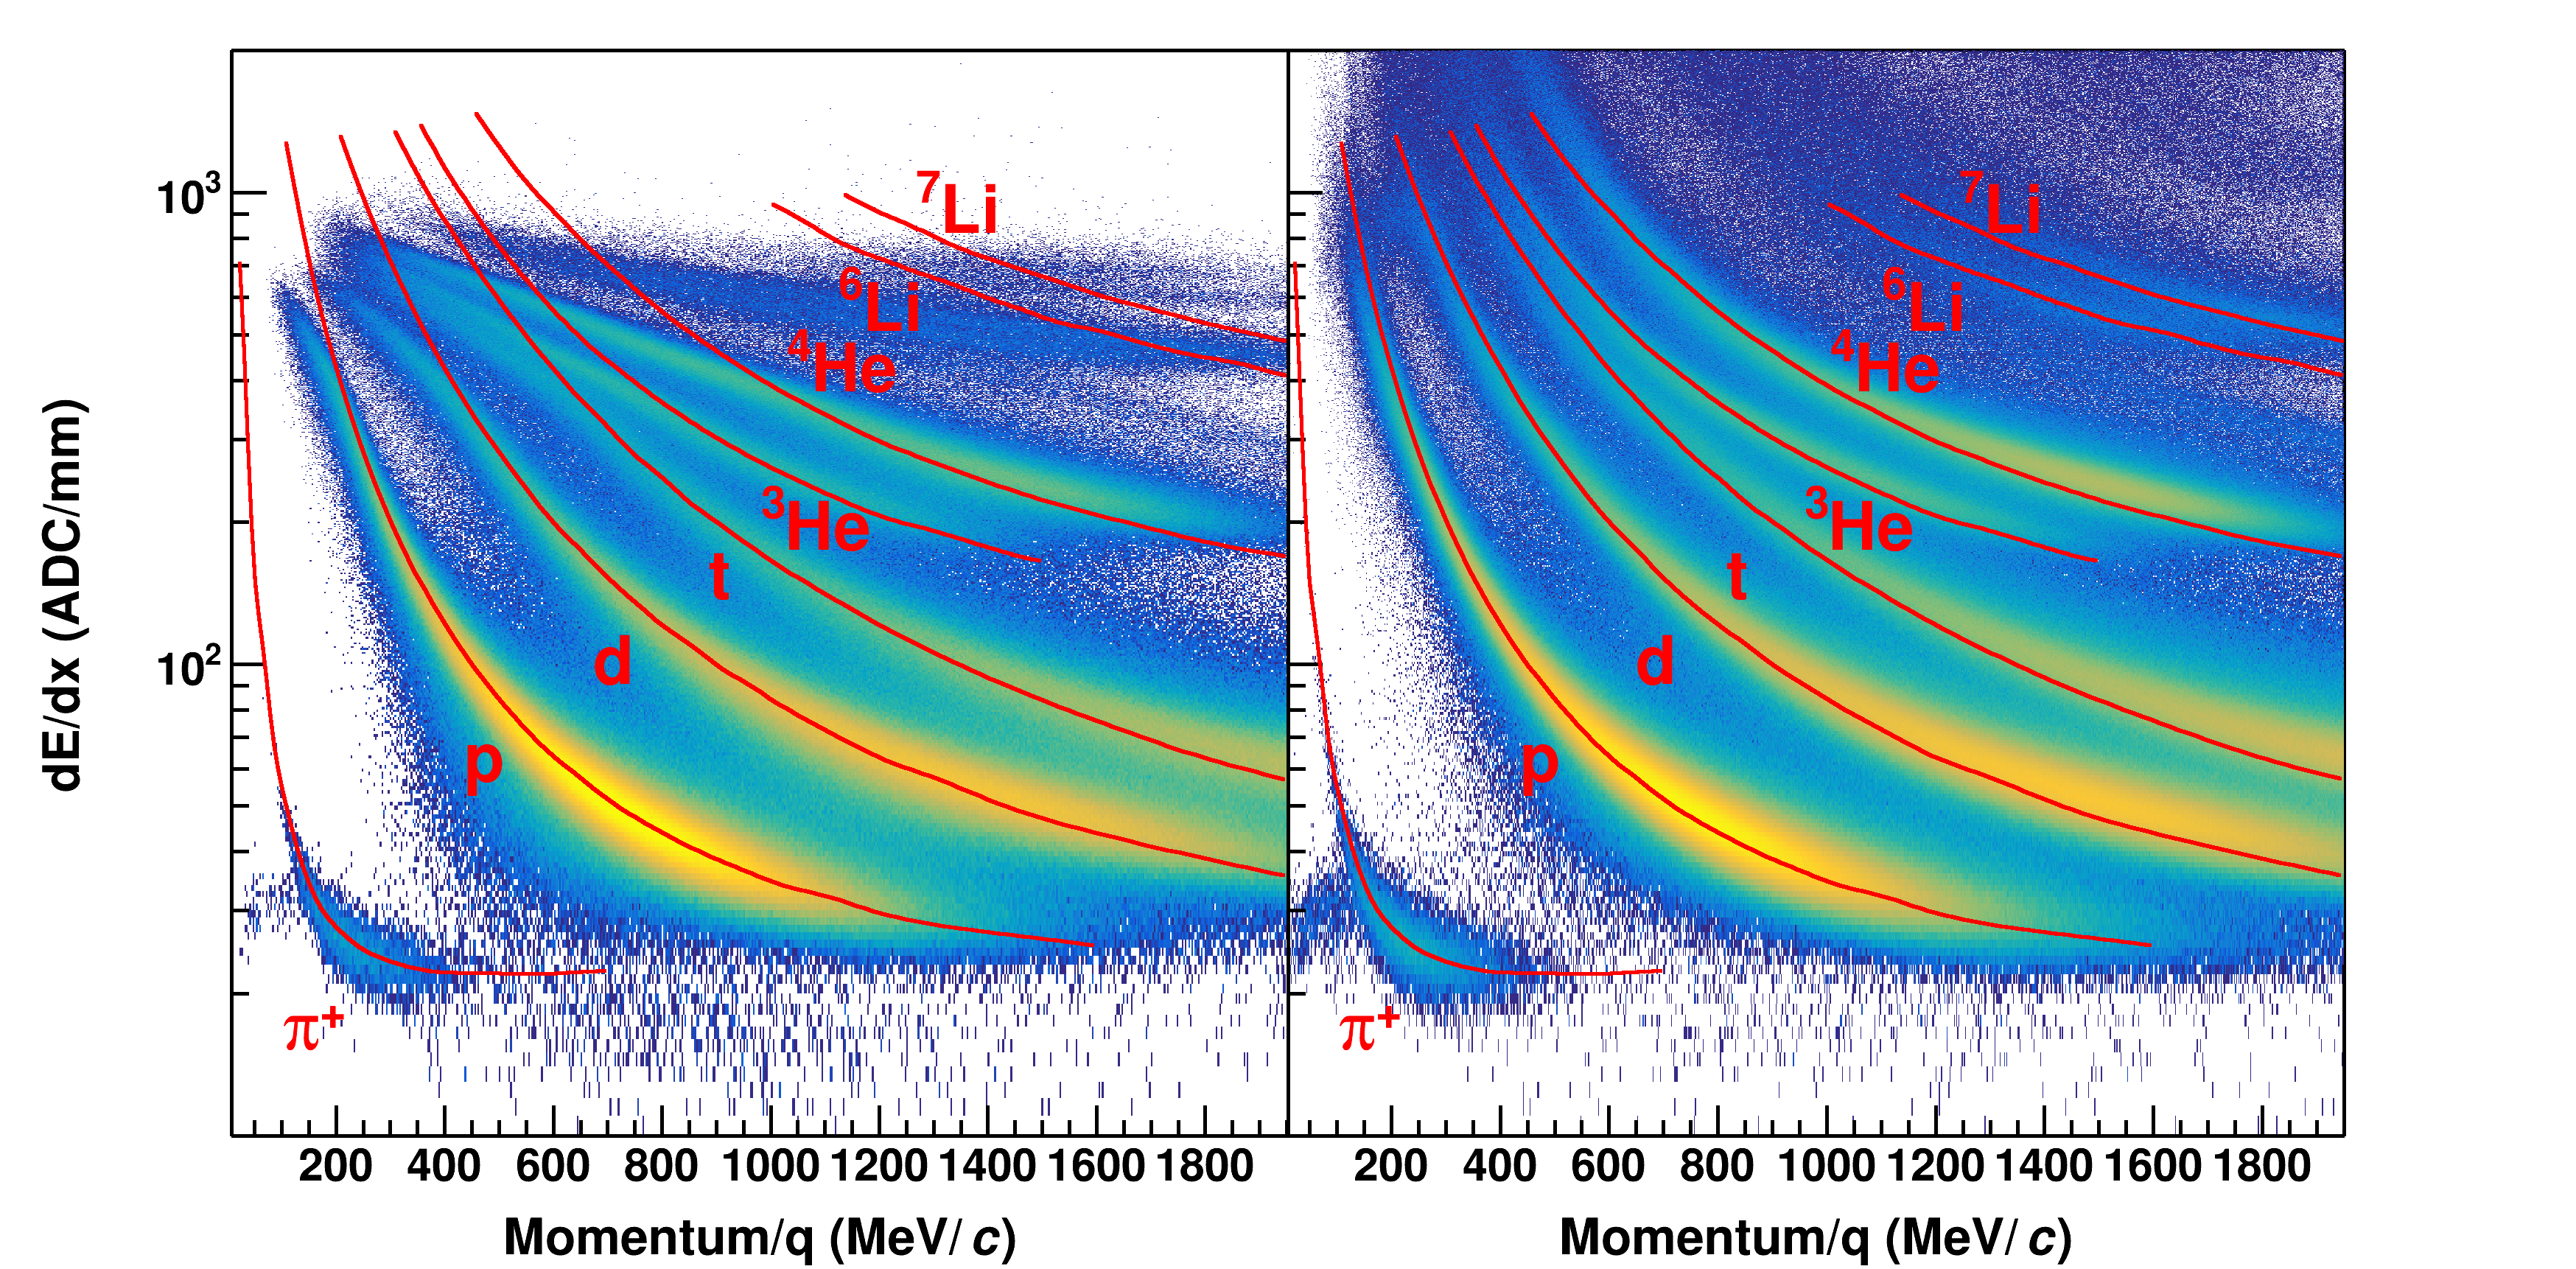
\includegraphics[width=\linewidth]{data_combine}
\caption{Uncorrected (left panel) and desaturated (right panel) collision data at polar angles of $\theta < 40^{\circ}$ and azimuthal angles between $-80^{\circ} < \phi < 80^{\circ}$}
\label{fig:data_combine}
\end{figure*}


\begin{figure*}[!htb]
\centering
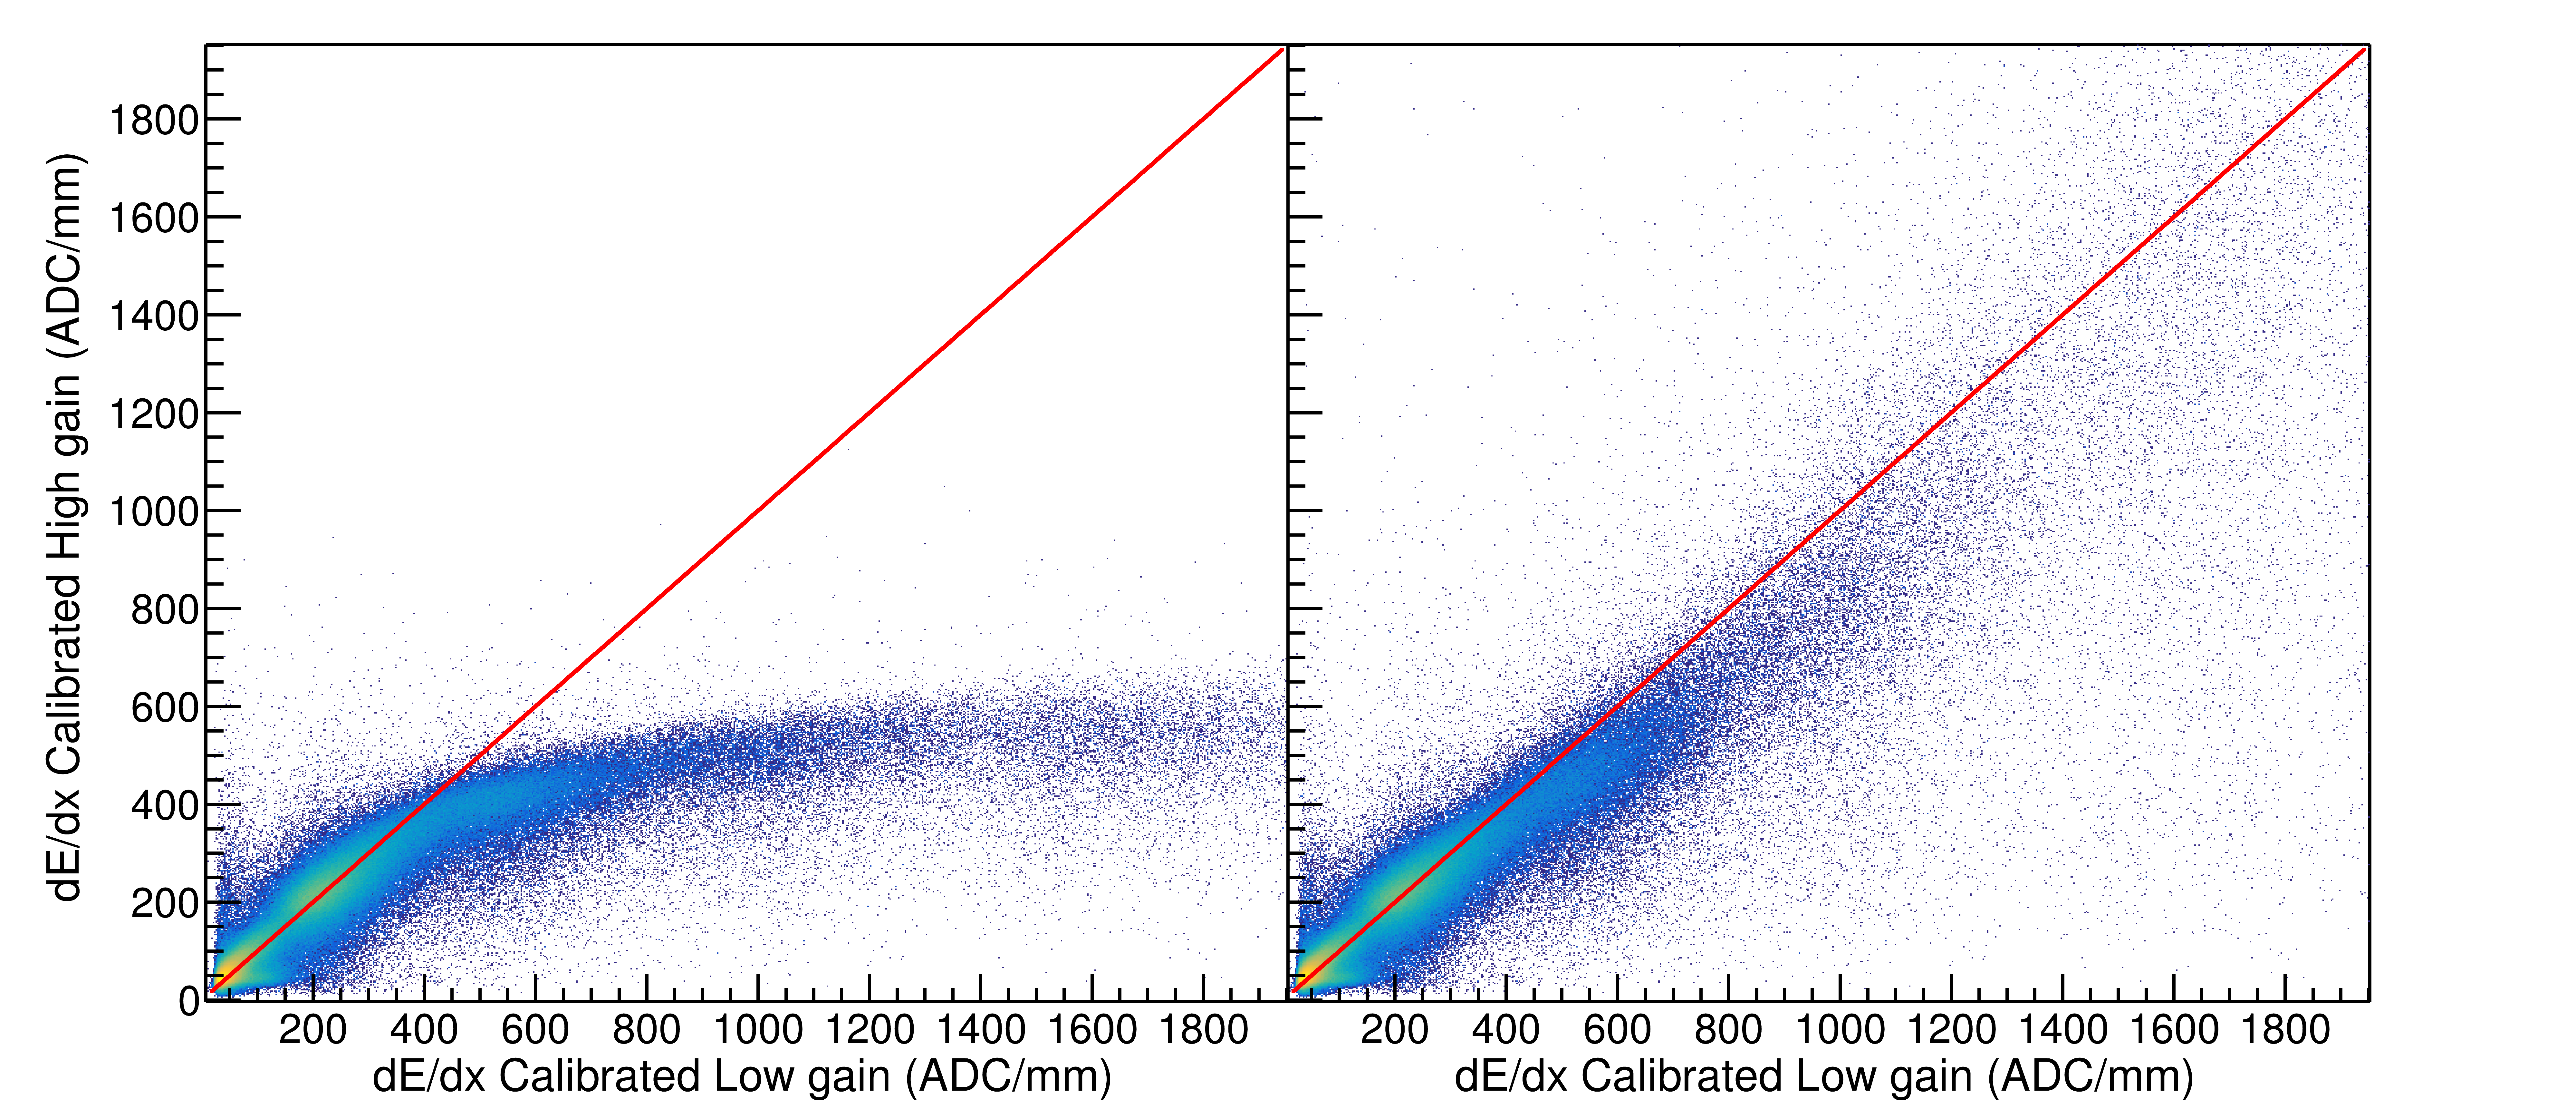
\includegraphics[width=\linewidth]{lowvshigh.png}
\caption{Uncorrected (left panel) and desaturated (right panel) collision data comparing the low gain region to the high gain anode regions of the TPC.}
\label{fig:lowvshigh}
\end{figure*}

To provide evidence of the success of this technique, we observe tracks which saturate pads in the high anode wire voltage region are not saturated in the low anode voltage region. While this desaturation technique avoids the need to lower the gain of any region, the low anode voltage region proved to be a direct measurement of the success of this technique.
 
Figure~\ref{fig:lowvshigh} shows the the $\langle dE/dx\rangle$ values of the high gain region compared with the calibrated low gain region. The effect of saturation can be seen in the high gain region for the uncorrected data above values of \SI{400}{ADC \per \milli\metre} where the values plateau, where as the low gain region still returns accurate values. Below this value the electronics are not saturated, and therefore the high and low gain sections agree. After applying the desaturation method, the correlation between the high and low gain sections is restored, as seen in Fig.~\ref{fig:lowvshigh}. From this comparison, we can approximate that the correction has corrected the high gain sections to agree with low gain sections to values of \SI{2000}{ADC \per \milli\metre}, increasing the dynamic range by a factor of a factor of at least 5.

The success of the desaturation becomes more clear when looking at the PID lines from the experimental data in Fig.~\ref{fig:data_combine}. In the following PID plots the red lines represent the most probable energy loss as given by Geant4 straggling functions. The uncorrected data in the left panel shows the effects of saturation, where the PID lines deviate significantly from their theoretical expectations starting at around \SI{400}{ADC \per \milli\metre}. After applying the desaturation technique -- in the right panel-- we see a large improvement, most notably for the He and Li particles, which suffer the most from saturation. Even the ${}^{6}Li$ and ${}^{7}Li$ particles can be separated and a more subtle improvement of the lighter particles (p, d, t), can also be seen at lower momenta. In these regions, there was little to no PID resolution before desaturation technique was applied.  


%Give some failures of the assumptions made

\subsection{Space Charge Corrections}
\label{sec:spacecharge}

%MAYBE ADD A LITTLE NAPKIN CALCULATION OF SPACE CHARGE TO SHOW ORDER OF EFFECT. 

As the particles passes through the gas inside of the field cage, they ionize the gas creating electron-ion pairs. The drift velocities of the ions are typically \SI{e4} times slower than electron drift velocities \cite{blumrol}. Because of this, any source of ions have the potential to build up in the drift volume, creating a positive space charge. If the space charge build up is large enough, it would distort drifting electrons therefore biasing the track momentum measurement. There are several regions of the TPC in which ions are created. The largest source of positive ions is created in the avalanche process near the anode wires. But as discussed in Section~\ref{sec:wireplanes}, the gating grid captures all of the ions from this region. The other source of ions come from the primary ionization produced by the beam and reaction products in the detector gas. The energy loss  $\langle dE/dx\rangle \propto Z^2$, where Z is the charge of the particle type. Because the charge of the un-reacted beam is around Z~50, the ionization due to the beam is a factor of \num{2e3} times that of the light charged particles which mostly are of charge Z~1. Therefore the ions resulting from the un-reacted beam is the largest source of positive ions in the TPC. 


%NEED TO PUT IN ABOUT THE GATING GRID LEAK 
 
 \begin{comment}
 
 \begin{table}[!htb] % not just 'h!'
\centering % not a center environment
\begin{tabular}{
  @{}
  l
  S[table-format=1.2]
  S[table-format=1.2]
  S[table-format=1.2]
  S[table-format=5.2]
  S[table-format=5.2]
  @{}
}
\toprule
Beam Energy Loss  &
 {${}^{132}$Sn} &
 {${}^{124}$Sn} &
 {${}^{112}$Sn} &
 {${}^{108}$Sn} &
  {Avg.}\\
  
\midrule
$\si{\kilo\eV\per\centi\meter}$ & 11.2   &.034  &5.43   &  903   &150     \\
\bottomrule
\end{tabular}

\caption{Average energy loss of each beam.}
\label{tb:beameloss}
\end{table}
\end{comment}


\begin{figure}[!htb]
\centering
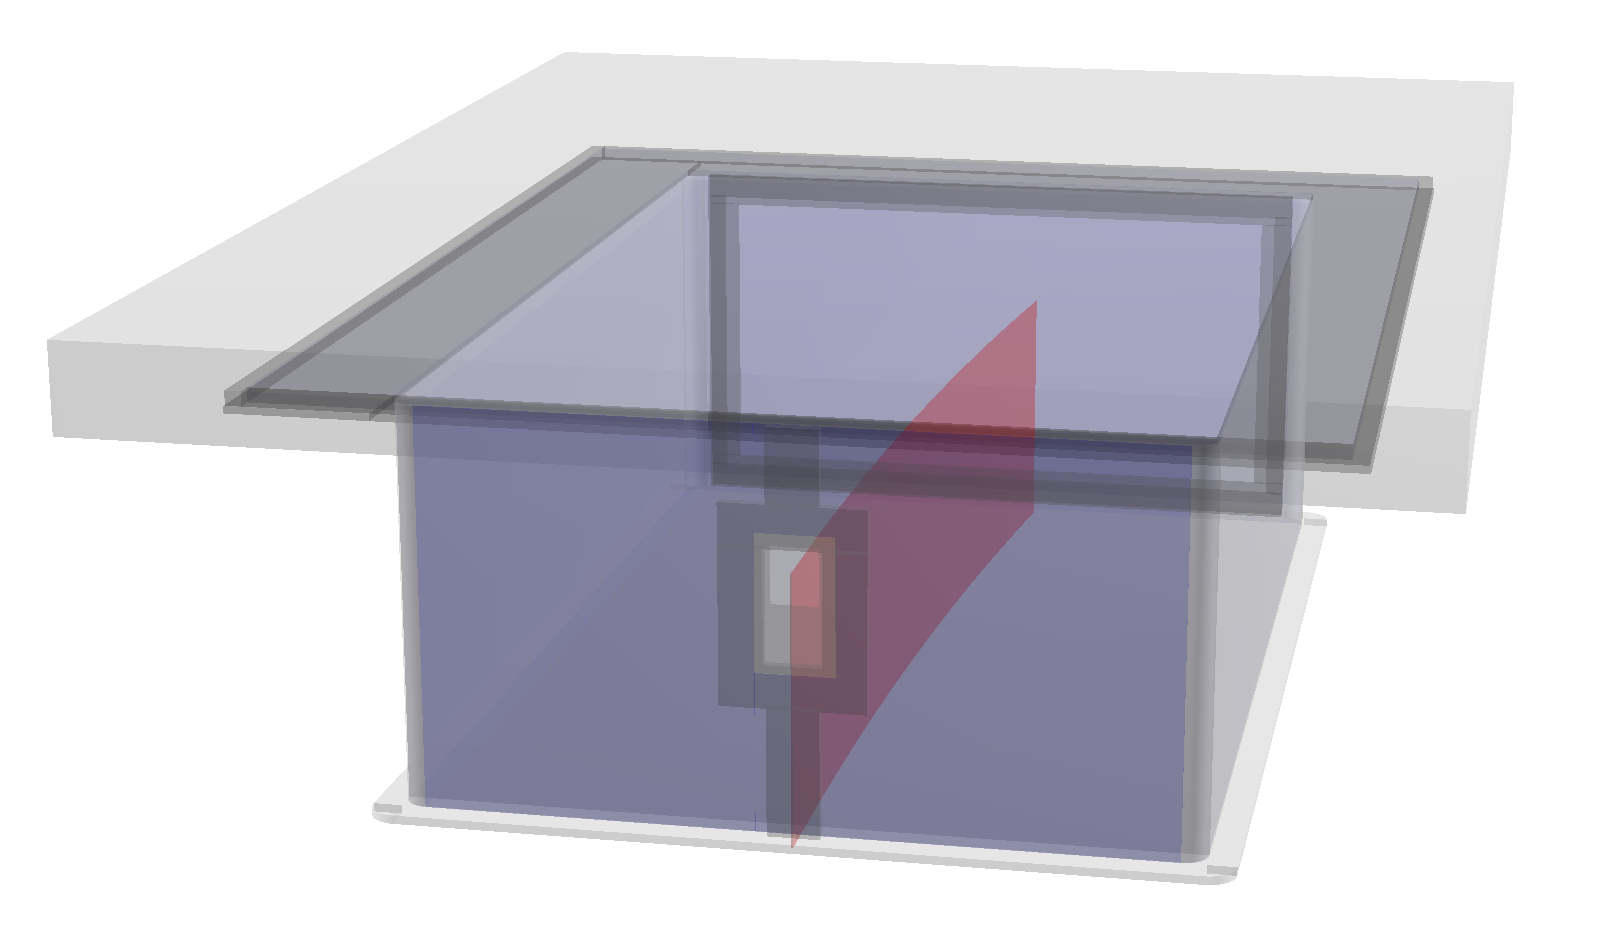
\includegraphics[width=\linewidth]{spacechg_cartoon.png}
\caption{Location of space charge in 132 Sn}
\label{fig:spacechg_cartoon}
\end{figure}


\begin{figure}[!htb]
\centering
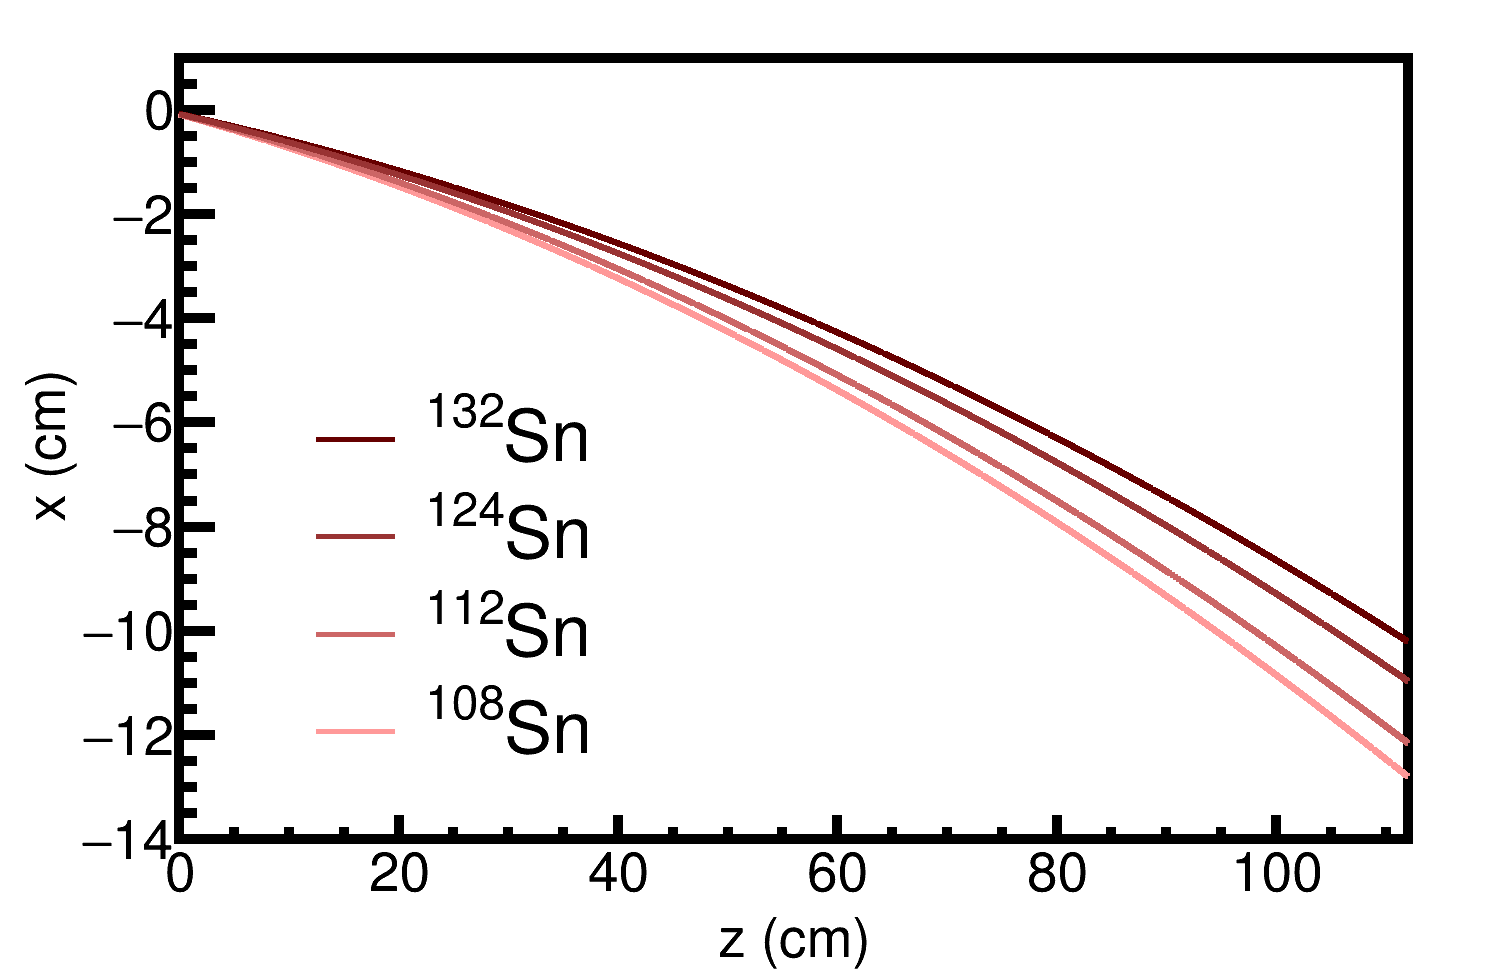
\includegraphics[width=\linewidth]{beampath.png}
\caption{Beam path of the experiments}
\label{fig:beampaths}
\end{figure}
 
 
 The beam is positioned about \SI{25}{\centi\metre} below the anode plane and \SI{29.6}{\centi\metre} above the cathode in the TPC. It takes electrons approximately 5\si{\micro\sec} to drift to the anode plane where as it takes the ions \num{5e4}\si{\micro\sec} to drift to the cathode. The beam rate in the experiment was approximately \SI{10}{\kilo\hertz}, which has an average occurrence of 1 beam every \SI{100}{\micro\sec}. This is  much shorter than the time it takes for the ions to terminate on the cathode plane, resulting in a build up of positive ions. Figure~\ref{fig:spacechg_cartoon} gives an idea of the shape of the sheet of space charge carved out by the beam path. The ions from each beam create a line charge which drifts towards the cathode with a constant velocity. The average distance between sequential ion paths is about \SI{25}{\micro\metre} apart, therefore we expect the average number of beam paths that make up the sheet charge is around \num{1440} tracks. Since the number of tracks in the sheet charge is large, and inter beam spacing is very small, we approximate the sheet charge as a uniform charge density. 
 
 The secondary beams entering the TPC are also composed of many secondary species which are impurities as will be discussed in Section~\ref{sec:beam}. Their charge values are mostly distributed around Z~50. Let us assume a beam of ${}^{132}$Sn where the energy loss in P10 gas, at \SI{270}{\MeVA}, is \SI{11.2}{\kilo\electronvolt\per\centi\metre}. From the total number of beams above, and the beam path length of \SI{135}{\centi\metre}, the estimated charge density would be on the order of \SI{3e-8}{\coulomb\per\metre\squared}. This gives us an understanding of the amount of space charge we should expect to see in the chamber. 
 

Once the amount of charge is known, the electric potential can be calculated by solving Poisson's equation, 

\begin{equation}
\nabla^2 \phi = \rho,
\end{equation}

 where $\phi$ is the electric potential and $\rho$ is the free charge. The numerical solution is provided by the Jacobi method \cite{poisson}, provided all 6 sides have defined Dirichlet boundary conditions for the potentials. We neglect the wire plane region since the drift details around it are not significant for the space charge effects we are discussing here. The pad plane and cathode are trivial, where the side walls of the field cage are given linearly varying potentials on the surface, such that the electric field is the same strength as the real TPC with no space charge present. Once the electric potential is solved, the electric field is simply the gradient of the potential  $\vec{E}= -\nabla \phi$. 
 
It has been shown before that the amount of space charge present in the chamber is related to observables such as the Distance-Of-Closest-Approach (DOCA) of each track to the vertex point \cite{starSC}. In the presence of no space charge, the DOCA distribution of each track would be a centered around the true vertex location. Because of the left right symmetry in the TPC, the space charge affects different regions of the TPC differently, and a bias is introduced to the measured vertex location and widening the distribution to vertex of each track.  

An example of the distortion map in the TPC is shown in Fig.~\ref{fig:sc_shift} where left-going tracks are shown in blue, and right-going tracks shown in green. The vectors show the direction of electron shift, and their magnitude have been magnified to show the detail. The dashed lines show the tracks under the influence of the space charge where left and right-going tracks are affected differently. Right-going tracks tend to higher momentum values and the left-going tracks going to lower momentum values, for positively charged particles.  
 

\begin{figure}[!htb]
\centering
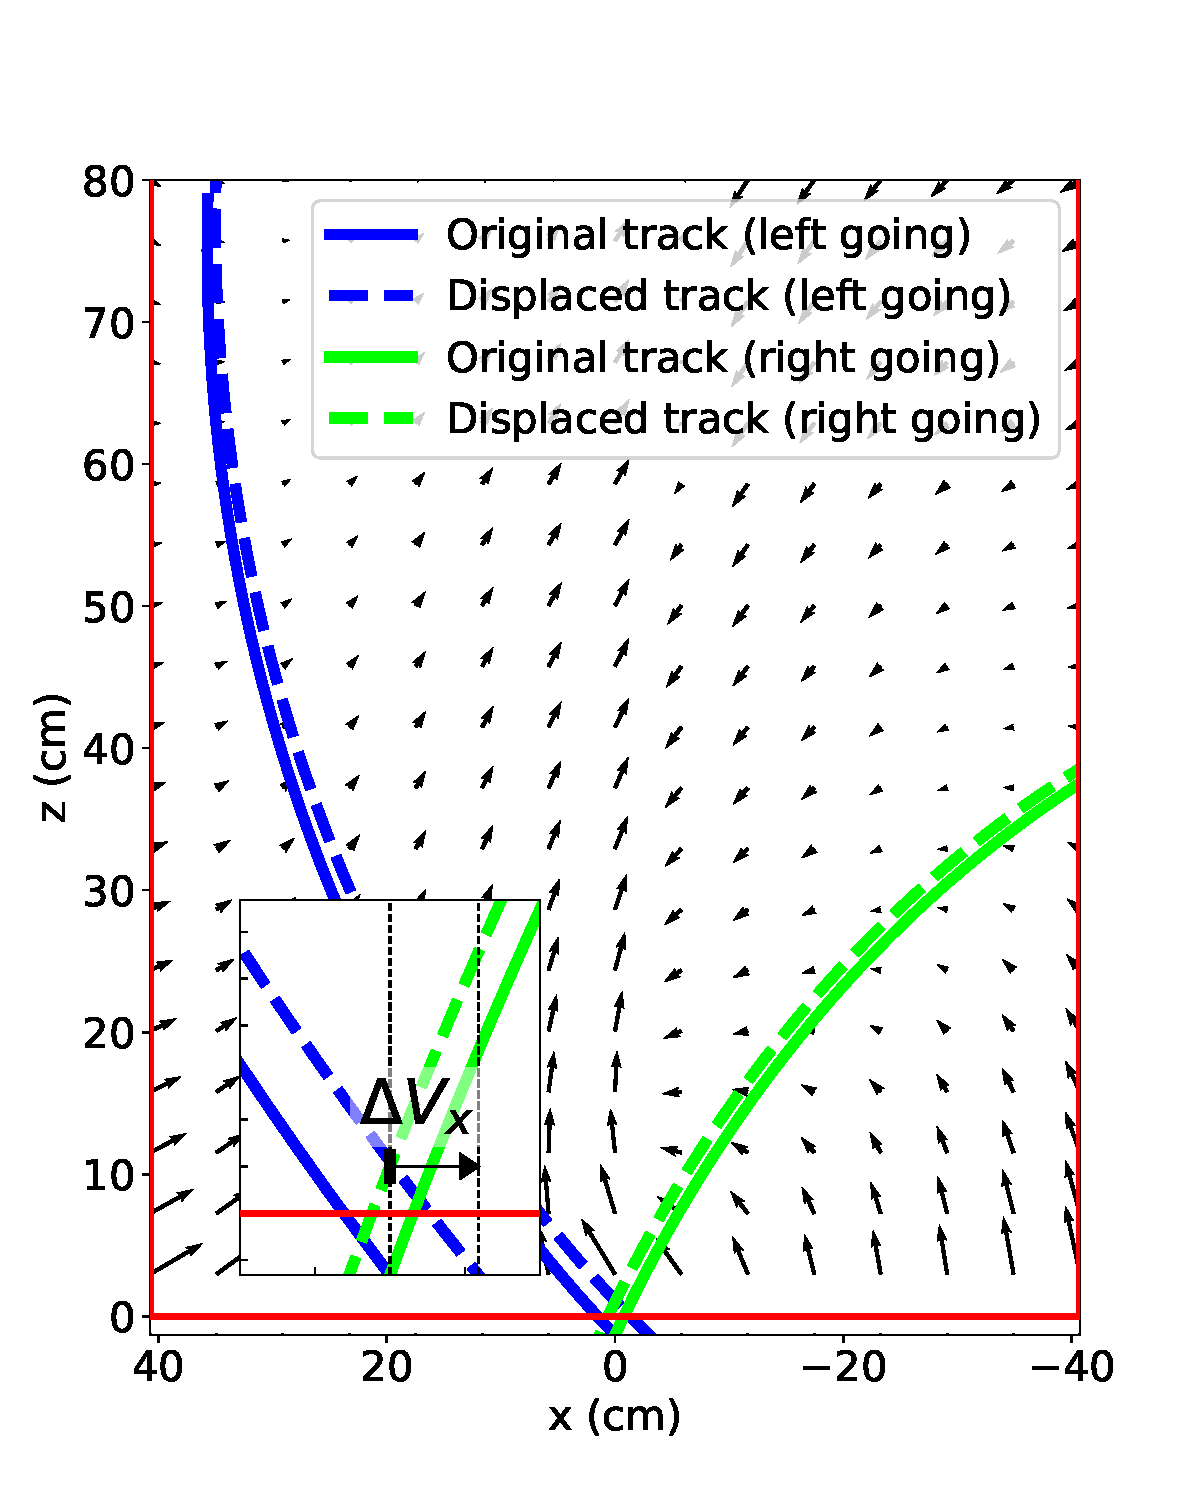
\includegraphics[scale=.5]{Effect_SC.pdf}
\caption{Example of the map of the electron shift. The effect is also shown on left-going (blue) and right-going (green) tracks. The original tracks are shown in the solid line and the shifted track in the dotted line.}
\label{fig:sc_shift}
\end{figure}

The inset figure of Fig.~\ref{fig:sc_shift} shows the effects of the space charge have on the x-component of the DOCA to the vertex. The DOCA distribution is displaced left-going track labeled by $\Delta\mathrm{V}_\mathrm{x}$, and in the opposite direction for right-going tracks. Figure~\ref{fig:VLR} shows the difference between right and left tracks as $\Delta\mathrm{V}_\mathrm{LR} = \Delta\mathrm{V}_\mathrm{x}^L - \Delta\mathrm{V}_\mathrm{x}^R$ , where  $V_x^L$ and $V_x^R$ are the most probable values of the DOCA distribution for left and right-going tracks respectively. As the space charge increases this value increases, where in the presence of no space charge, we would expect exactly $\Delta\mathrm{V}_\mathrm{LR} = 0$. 

\begin{figure}[!htb]
\centering
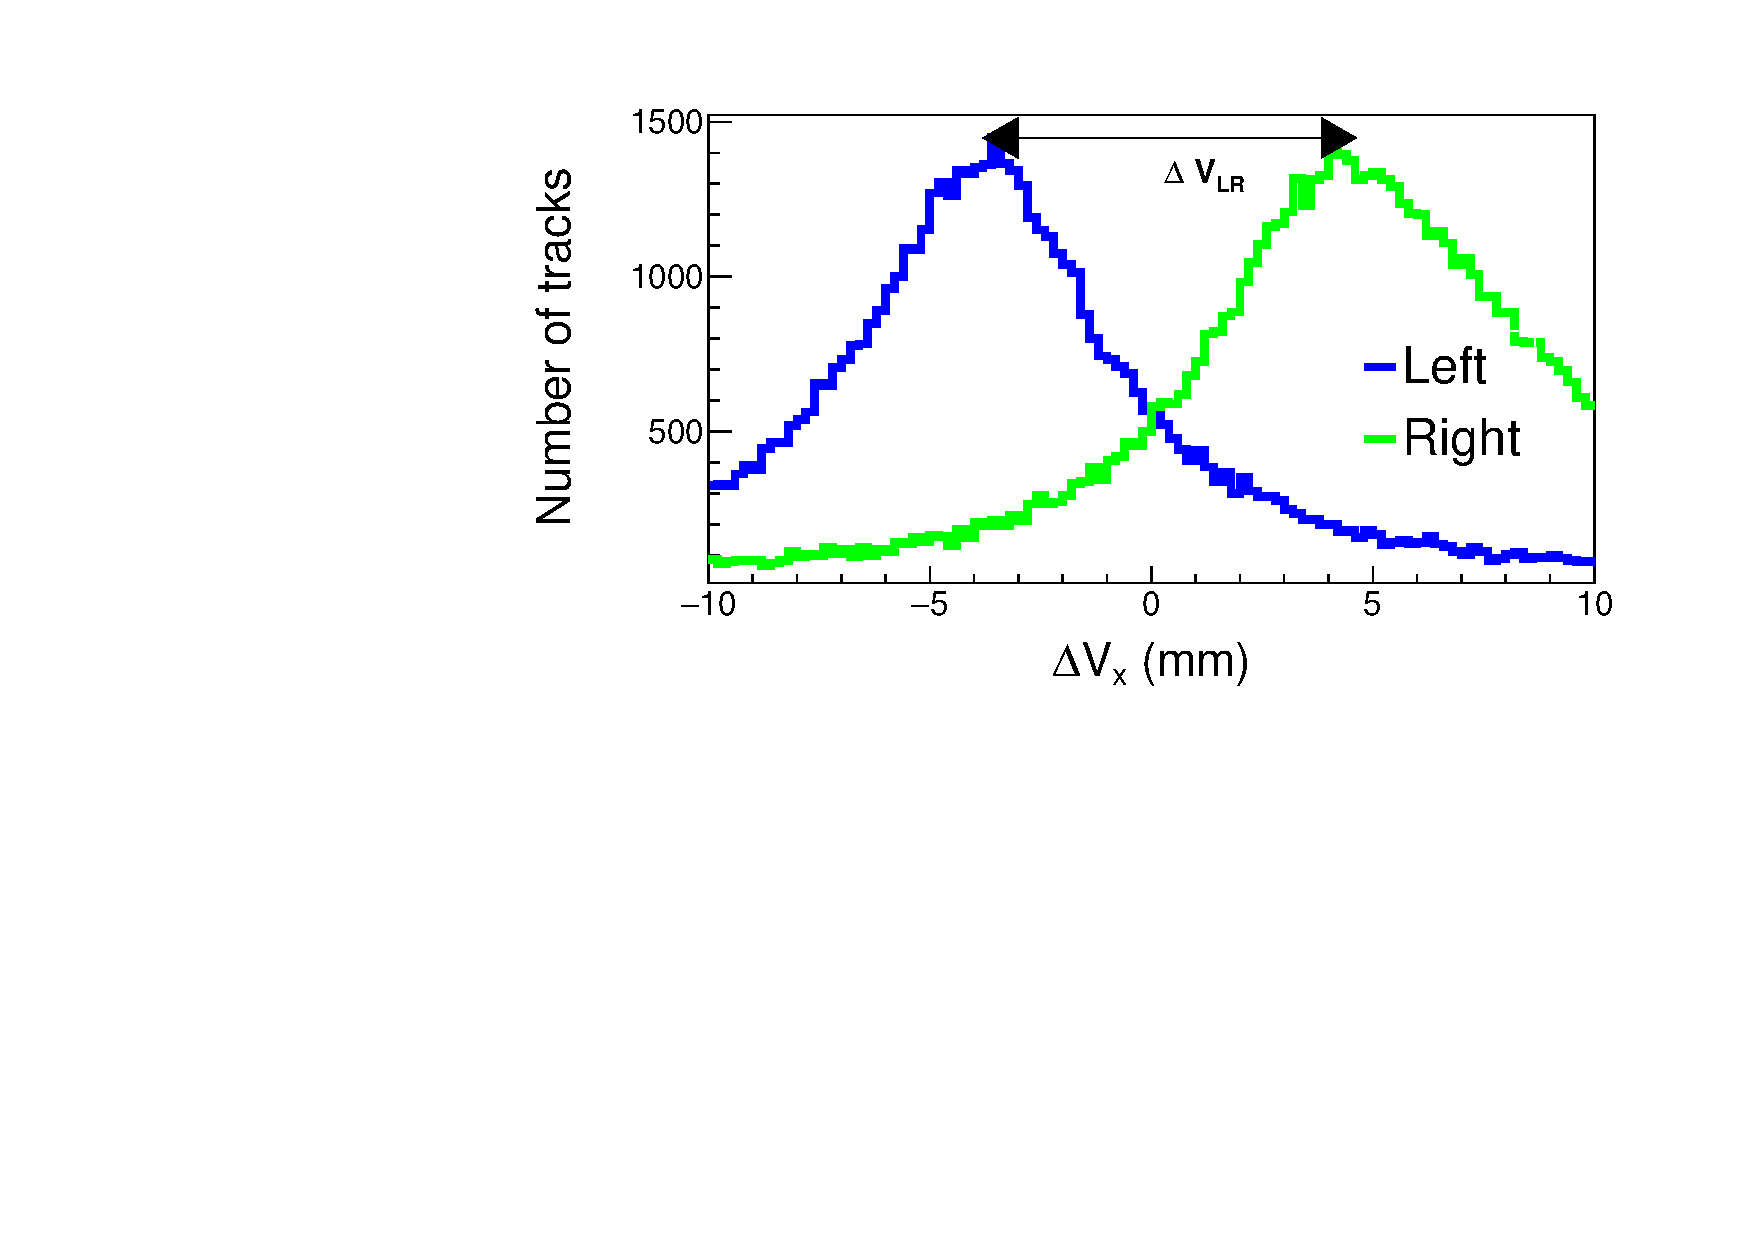
\includegraphics[scale=.5]{DVTP_raw.pdf}
\caption{$\Delta\mathrm{V}_\mathrm{x}$ distribution for left-going and right-going tracks. }
\label{fig:VLR}
\end{figure}



\begin{figure}[!htb]
\centering
\includegraphics[width=\linewidth]{VLR_beamrate.png}
\caption{ $\Delta V_{LR}$ versus the beam rate for all systems with the fitted function.}
\label{fig:VLR_br}
\end{figure}



\begin{figure}[!htb]
\centering
\includegraphics[width=\linewidth]{sc_beamrate.png}
\caption{Space charge fit function versus the beam rate for all systems. These are the assumed functions we use for interpolating the space charge value from the beam rate.}
\label{fig:spacechg_br_all}
\end{figure}

The average beam rate was recorded in each experimental run and slightly varied from run to run due to beam production variations. The amount of space charge present in the field cage is directly proportional to the beam rate and therefore $\Delta\mathrm{V}_\mathrm{LR}$.  Fig.~\ref{fig:VLR_br} shows the relation between the measured $\Delta\mathrm{V}_\mathrm{LR}$ values and the estimated beam rate. 

The only parameter in the space charge correction algorithm is the surface charge density $\sigma_{\mathrm{SC}}$. By varying $\sigma_{\mathrm{SC}}$ for a wide range of values, the $\Delta\mathrm{V}_\mathrm{LR}$ observable is measured and plotted in the left panel of Fig.~\ref{fig:spacechg_relation}. The values are linearly fit to find the solution of the surface charge density which gives $\Delta\mathrm{V}_\mathrm{LR} = 0$, which is then taken to be the estimate for the average amount of space charge present in a given run.

This is done for several runs which vary in beam intensity. Since the surface charge density is proportional to the beam rate, a linear fit gives good agreement for interpolating the surface charge values as a function of beam rate. Figure~\ref{fig:spacechg_relation} shows the relation of the dependence of the space charge as a function of beam rate for the ${}^{132}$Sn system.

\begin{figure}[!htb]
\includegraphics[width=\linewidth]{SC_Relation.pdf}
\caption{Relationship between the observable  $\Delta\mathrm{V}_\mathrm{LR}$ and the estimated charge density, and the beam intensity for each run. The blue and green line represents two separate runs at different beam intensities. The condition for  $\Delta\mathrm{V}_\mathrm{LR} = 0$ is solved for for each run. These values are then plotted against the beam intensity where finally a linear fit provides the interpolation for all beam intensities in between.}
\label{fig:spacechg_relation}
\end{figure}


Following this algorithm, the space charge can be estimated for each run and system. Figure~\ref{fig:scDensity} shows the summary of the extracted space charge values for each secondary beam. The linear fits relating the space charge density to the beam rate for each system is shown in Fig.~\ref{fig:spacechg_br_all} where the space charge value is inferred from the measured beam rate. Notice that in the $\tin{112}{124}$ system we assume a constant the space charge correction, since the variation in $\Delta\mathrm{V}_\mathrm{LR}$ rate did not span a large enough range to warrant a more detailed analysis. 

To reduce the need to compute a new electric field for each space charge value, notice that $\vec{E}\propto \rho$. We can therefore solve the electric field for a certain reference charge value $\rho_o$, and scale the solution for any other free charge $\rho$ linearly by the ratio $\rho/\rho_o$. The full magnetic field map is provided by the SAMURAI collaboration \cite{magnet}. The velocity field map is calculated following Eq.~\ref{eq:elecdrift}, where the electron drift through this velocity map is propagated by using a time stepped $\mathrm{4}^{\mathrm{th}}$-Order Runge-Kutta integration from a certain starting point.
  
 The correction map is calculated in the inverse method, starting from the anode wires and location on the pad-plane (x,z), and stepping backward in time in the Runge-Kutta integration through the velocity field map until the electron reaches the measured y-position. This is done over a 3-dimensional grid where points in between are interpolated by a tri-linear interpolation. The measured clusters value (x,y,z) position is input into the correction map which outputs the interpolated correction values $dx$ and $dz$ which correspond to that cluster. The cluster position is then shifted to new positions $x\textprime = x + dx$ and $z\textprime = z + dz$.
 

%What is the best figure to put in? VLR vs Charge density? 
%estimate of the error of VLR and how it corresponds to charge density

\begin{figure}[!htb]
\includegraphics[width=\linewidth]{spaceChgDensity.png}
\caption{Distribution of estimated space charge densities for each beam type.}
\label{fig:scDensity}
\end{figure}



\begin{figure}[!htb]
\includegraphics[width=\linewidth]{VLRresidual.png}
\caption{Residuals in the fitted line of $\Delta V_{LR}$ observable for all systems.}
\label{fig:vlrResidual}
\end{figure}

Adding the BDC vertex greatly improves the momentum resolution of the track fitting.  Since we know that the space charge affects right and left-going tracks differently, both tracks appear to diverge from the original vertex location appearing to no longer originate from the BDC vertex which is independent of the space charge effects. Without correcting for the space charge effects adding the BDC introduces a systematic shift in the momentum when comparing right and left-going tracks as compared with the momentum value before adding the BDC. For tracks at polar angles of $\theta_{Lab} < \ang{40}$, the disagreement between momentum values with and without the BDC are much less obvious. This is because for small deviations in the track -- at smaller polar angles -- leads to small deviations at the target location. Therefore the momentum without does not disagree as much as with the BDC point as shown in Fig.~\ref{fig:mom_S_before}. Figure~\ref{fig:mom_L_before} shows the momentum value of tracks going at polar angles of $\theta > 40 \deg$ which are more sensitive to small changes in the track -- corresponding to larger deviations at the target location. Therefore we get large systematic shifts in the momentum after including the BDC. After correcting for the space charge effects, the reconstructed momentum value agrees with or without the BDC included, for both  polar angles $\theta_{Lab} < \ang{40}$ and $\theta_{Lab} > \ang{40}$, as seen in Fig.~\ref{fig:mom_S_after} and Fig.~\ref{fig:mom_L_after} respectively. 


\begin{figure}[!htb]%
    \centering
    \subfloat[Compare the momentum before and after including the BDC vertex for tracks with $\theta_{Lab} < \ang{40}$, before the space charge correciton.]{{\includegraphics[width=.45\textwidth,valign=c]{BDC_P_small_angle.pdf} \label{fig:psa0}}}%
    \qquad
    \subfloat[Comparison of the momentum before and after including the BDC vertex for tracks with $\theta_{Lab} > \ang{40}$, before the space charge correction.]{{\includegraphics[width=.45\textwidth,valign=c]{BDC_P_large_angle.pdf} \label{fig:mom_L_before}}}\\
    \subfloat[Compare the momentum before and after including the BDC vertex for tracks with $\theta_{Lab} < \ang{40}$, after the space charge correction.]{{\includegraphics[width=.45\textwidth,valign=c]{BDC_P_aftercor_small_angle.pdf} \label{fig:mom_S_after}}}%
    \qquad
    \subfloat[Compare the momentum before and after including the BDC vertex for tracks with $\theta_{Lab} < \ang{40}$, after the space charge correction.]{{\includegraphics[width=.45\textwidth,valign=c]{BDC_P_aftercor_large_angle.pdf}  \label{fig:mom_L_after}}}%

 \label{fig:mom_sc}
\end{figure}



\begin{figure}[!htb]%
    \centering
    \subfloat[$\tin{132}{123}$ system.]{{\includegraphics[width=\textwidth,valign=c]{sn132_SC} \label{fig:132momdist_sc}}}%
    \qquad
    \subfloat[$\tin{108}{112}$ system.]{{\includegraphics[width=\textwidth,valign=c]{sn108_SC} \label{fig:108momdist_sc}}}%
	\caption{Momentum distributions of the Left and Right sides of the TPC for $\pi^+$ and $\pi^-$ particles.}
	\label{fig:sc_momdist}
\end{figure}



This is one of the arguments for the success of the space charge correction task. Recall that only the relative distance between left and right-going tracks was minimized, and there was no guarantee that the corrected tracks coincide with the absolute BDC position at the target. The others being the agreement with the expected cocktail calibration beam as described in Section~\ref{sec:cocktail}.

Here we will discuss some of the final results of the pion kinetic energy spectrum as it pertains to the verification of the space charge analysis. The details of the pion PID analysis will be discussed in detail in Section~\ref{sec:pid}. Figure~\ref{fig:sc_momdist} shows the $\pi^+$ and $\pi^-$ kinetic energy distributions in the center of mass system for the $\tin{132}{124}$ and $\tin{108}{112}$ systems. The momentum distributions are split into the beam-left and beam-right side of the TPC. For central collisions, one would expect no difference between the two momentum distributions due to the symmetry of the emission. As seen in the left panels of both figures, the data before the space charge correction is shown, where as in the right panels the data after the space charge correction is shown. There is a significant improvement in the matching of the left and right side momentum distributions for both charged pion species, in both systems, especially for the high energy tail of the pions. It is remarkable that the DOCA observable provided a good enough measure of the average space charge in the chamber. There is no reason to assume correcting the DOCA distribution would correct the momentum distribution. This is the strongest evidence to the success of the space charge correction.



\section{CoBo timing correction}
The arrival time of signals originating from each pad may differ due to timing delays in the electronics and cabling. These timing differences affect the y-position measurement of each track. By measuring the y-direction track residuals, we find the timing differences correspond to about $\pm$\SI{2}{\milli\metre} in position differences. The timing difference is stable for each pad across several runs. 

\begin{figure}[!htb]%
    \centering
    \subfloat[]{{\includegraphics[width=.3\textwidth,valign=c]{run2907_yoffset6before_row_at_layer10.png} \label{}}}%
    \qquad
    \subfloat[]{{\includegraphics[width=.3\textwidth,valign=c]{run2907_yoffset5before_row_at_layer30.png} \label{}}}%
    \subfloat[]{{\includegraphics[width=.3\textwidth,valign=c]{run2907_yoffset4before_row_at_layer50.png} \label{}}}%\\
    
    \subfloat[]{{\includegraphics[width=.3\textwidth,valign=c]{run2907_yoffset6after_row_at_layer10.png} \label{}}}%
	\qquad
    \subfloat[]{{\includegraphics[width=.3\textwidth,valign=c]{run2907_yoffset5after_row_at_layer30.png} \label{}}}%
    \subfloat[]{{\includegraphics[width=.3\textwidth,valign=c]{run2907_yoffset4after_row_at_layer50.png} \label{}}}%

	\caption{Cobo timing correction for three different layers. One singe pad is represented by a unique layer and row number. The $dy$ residual of the track fitting shows, in the upper panel, that there is a timing calibration issue. This offset is fixed over several runs for a given pad. Therefore we can correct using a time correction map for each pad; the bottom panels show the distribution after correction. }
  	\label{fig:coboCorr}
\end{figure}



\begin{figure}[!htb]%
    \centering
    \subfloat[Before applying the timing correction.]{{\includegraphics[width=.46\textwidth,valign=c]{run2905_yoffset1before_all.jpg} \label{fig:yoff_allBefore}}}%
    \qquad
    \subfloat[After applying the timing correction.]{{\includegraphics[width=.46\textwidth,valign=c]{run2905_yoffset1after_all.png} \label{fig:yoff_allAfter}}}%

    \caption{Y-residual distributions for all pads.}
	\label{fig:yoff}
\end{figure}


 Figure~\ref{fig:coboCorr} shows the y-residuals, across all the rows, for three different layers; where each row here represents a unique pad with a row and layer ID. Before the correction, one can see large deviations in the y-residuals which correspond to timing differences. The mean value of the y-residual distribution is fitted and an inverse correction map is constructed for each pad. The data is then reconstructed subtracting value from the inverse map, $dy$, for each pad. The resulting corrected distribution is shown in Fig.~\ref{fig:coboCorr} for the same layer set. Figure~\ref{fig:yoff} also show the summary of all the pads before the correction and after the correction. There is a significant improvement in the width of the distribution going from \SI{1.5}{\milli\metre} to \SI{0.6}{\milli\metre}. 



%Reference appendix for poisson solver 
%Tables for ion drift velocity in P-10 Gas reference Sauli
%Figure of sDAC or POCA 
%Figure of cartoon of what is happening to tracks
%Figure of correction map in TPC and MC map 
%Figure of before and after correction BDC vs reco momentum
%Figure of track residuals before and after?



\section{Monte Carlo Simulation}
\label{sec:monteCarlo}

The MC simulation is composed of two separate simulations. The first simulation utilizes Geant4 to simulate the interactions of a particle passing through the various materials in the TPC. A scale model of the field cage was made, and the correct materials types were put in, with the correct gas mixture and density of P-10 gas at a density of 1 atm. The magnetic field map of the SAMURAI dipole magnet was also imported into Geant4 as well after assuming rotational symmetry along the axis perpendicular to the pole face -- since only 1/4 of the magnet was simulated. Along with the energy loss and particle transport, Geant4 also handles multiple scattering, and particle decays, which are all important effects especially for calculating the inefficiencies of pions. The output of Geant4 is a series of energy loss points which contain the amount of energy lost in $\si{\kilo\electronvolt\per\centi\metre}$ and the location of the energy loss in Cartesian space $(x,y,z)$. 

In the second part of the MC simulation, the physical processes of the TPC measurement are simulated, such as the electron drift, avalanche process, and all processes involved in the signal creation in the electronics. This is separated into three software tasks, the drift, pad response, and electronics tasks. In the following section we will discuss these tasks in more detail, the discussion of Geant4 is not covered here and the reader is refered to \cite{geant4}.  

\subsection{Drift Task}
 
 The first step of the drift task is to convert the primary and secondary ionization points of the MC track provided by Geant4 into electrons. The average number of electrons created in a gaseous detector,$N_{e^-}$, can be described as,
\begin{equation}
N_{e^{-}} =  \frac{\Delta E}{I},
\label{eq:kev2el}
\end{equation}
 
where $I$ is the ionization coefficient of P10 gas (Table~\ref{tb:gas}) and $\Delta E$ is the energy loss deposited. Each electron is then drifted along the electric field lines, under the assumption  that the electric field is uniform, which is true for most of the pad plane region. The total length drifted from the initial primary ionization point to the final anode wire is $L_{anode}$. 

\begin{table*}\centering
\ra{1.3}
\begin{tabular}{@{}rr@{}}\toprule 
\multicolumn{2}{c}{Electron Transport Gas Properties} \\
 \midrule
Drift velocity & 5.53 $\si{\centi\meter\per\micro\second}$\\
Transverse diffusion & 240 $\si{\micro \meter \centi\meter}^{-1/2}$\\
Longitudinal diffusion &  340 $\si{\micro \meter \centi\meter}^{-1/2}$\\
Gas Ionization & 26.2 $\si{\eV}$\\
\bottomrule
\end{tabular}
\caption{An overview of electron drift properties in P10 gas.}
\label{tb:gas}
\end{table*}

Drifting electrons frequently collide with the detector gas causing them to change direction. This stochastic motion is  described by a diffusion process occurring along the direction of travel (longitudinal) and transverse to the motion. The longitudinal ($c_{l}$) and transverse ($c_{t}$) diffusion coefficients are determined by Garfield++ calculation  \cite{garfield++} in the presence of a \SI{0.5}{\tesla} magnetic field, listed in Tb.~\ref{tb:gas}. The diffusion process is modeled by randomly sampling from a Gaussian distributions describing the diffusion in both of the directions. The random displacement vector is then added to the final position of the electron. The deviation in the transverse direction, $dr$, is randomly sampled from the distribution,

\begin{equation}
dr = e^{-\frac{r^2}{2\sigma_{t}^2}},
\end{equation}

where $\sigma_{t}=c_{t}\cdot\sqrt{L_{anode}}$.The transverse Cartesian directions can be written as $dx = dr \cdot \cos(\alpha)$ and $dz = dr \cdot \sin(\alpha)$, where $\alpha$ is a random angle from 0 to 2$\pi$, since there is no preferential angle  of emission in the transverse plane. The shift associated with the longitudinal diffusion, $dl$, is randomly sampled from, 

\begin{equation}
dl = e^{-\frac{t^2}{2\sigma_{l}^2}},
\end{equation}

where $\sigma_{l}=c_{l}\cdot\sqrt{L_{anode}}$. 

The final position of the electron along the wire is calculated  $x' = x + dx$. The electron will terminate on the closest anode wire, that is the anode wire that is closest to the shifted z-position $z\textprime = z + dz$, and the final electron z position is then updated to be the same as the anode wire it terminated on. The total drift time of the electron $t$ is calculated as,

\begin{equation}
 t = \frac{L_{anode} + dl}{v_d} + t_{offset},
 \label{eq:electronTime}
\end{equation}
 
where $v_d$ is the drift velocity. The parameter $t_{offset} = \SI{49.92}{\nano\second}$ is to allow for an alignment of the MC time bucket spectrum with the data. This is because the y-position corresponding to $t=0$ in the data time bucket spectra, does not correspond to the same position in the MC.  

Once the electrons have terminated on a particular wire, the avalanche process is simulated. The total number of electrons produced in the avalanche process of a single electron was simulated in Garfield++ and discussed in Section~\ref{sec:wireplanes} for the anode wire voltages used in the experiment. The number of electrons produced in the avalanche is randomly sampled from the Polya distribution  corresponding to the anode wire sections the electron terminated. The number of electrons produced is stored as a gain factor in that particular electron, instead of multiple instances of the original electron, to save storage space and computation time. 

%We assume that the lateral movement along the wire arising form $\vec{E}\times\vec{B}$ effect near the wire is negligible as compared with diffusion and other effects described later. 

It is worth mentioning there is the possibility to simulate the space charge effects in this task. This is not used for calculating the response of the TPC for efficiency calculations since it is a trivial exercise to input the space charge map only to then correct for it using the inverse map.  

\subsection{Pad Response Task}
The total charge of each avalanche is then distributed according to the pad response function (PRF) described in Section~\ref{sec:prf}. The PRF is simulated as the double integral of a 2-dimensional Gaussian. The final output charge on all the pads are the superposition of the PRFs of all drifted electrons. The MC PRF is expressed as, 

\begin{equation}
PRF(x,z) = \iint e^{-\frac{(x-x_o)^2}{2\sigma_x^2}} e^{-\frac{(z-z_o)^2}{2\sigma_z^2}}dxdz,
\end{equation}

where $\sigma_x = 3.4$ and $\sigma_z = 3.5$, and $x_0$ and $z_0$ are the final position of the drifted electron. The Gaussian width parameters were determined through an iterative comparison matching the PRFs of the MC and experimental data sets. 


\subsection{Electronics Task}

The purpose of the electronics task is to simulate the electronics response to a particular charge induced on each pad, converting charge into ADC channels. In a simplified picture, the induced charge on each pad goes through a pre-amplifier and shaping amplifier which determine the final pulse shape that is read out. The pulse shape did not change significantly in any circumstance, such as pulse height, data type, or particle type, as long as the electronics settings were fixed. This allows us to assume the pulse shape is constant and can be described by two variables, the height of the pulse, $Q$, and the starting time bucket of the pulse, $t_o$. The starting time of the pulse is defined as the time at 10\% pulse height, on the rising edge. The shape of the pulse depends on the shaping time constant which was set to \SI{117}{\nano\second} for the data analyzed here. Figure~\ref{fig:pulseshape} shows the pulse shape which was extracted from the experimental signals in the data. These were signals that did not saturate the electronics and was averaged over a wide range of ADC values. Here it is normalized so the maximum height is 1. 



\begin{figure}[!htb]
    \centering       
    \includegraphics[width=\linewidth]{satpulse.png} 
    \caption{The standard pulse shape and saturated pulse shape extracted from the experimental data, and used in the MC software.}
    \label{fig:pulseshape}
\end{figure}


Converting the charge in each pad into the height of the ADC response in the electronics is calculated as, 

\begin{equation}
Q = f_G  N_{e}  \cdot e \cdot\frac{ADC_{max} - ADC_{pedestal}}{f_c}
\label{eq:etoADC}
\end{equation},

where $e$ is the fundamental charge of the electron in $\si{\femto \coulomb}$, $N_{e}$ is the total number of avalanche electrons, $ADC_{pedestal}$) is the pedestal (300 ADC, $\mathrm{ADC_{Max}}$ is the maximum allowed ADC value (4096), and $f_c$ is the dynamic range setting (\SI{120}{\femto\coulomb}). The pulse shape given in Fig.~\ref{fig:pulseshape} is multiplied by the pulse height $Q$ giving the full time bucket estimate of the TPC response. Random Gaussian noise is added to each time bucket, where the root-mean-squared value of the electronics noise was measured to be around 6 ADC. The timing information of the pulse is calculated from Eq.~\ref{eq:electronTime}. The coefficient $f_G$ corresponds to a factor which allows for fine tuning of the ADC calibration. This factor is calculated by

\begin{equation}
f_G^p = \frac{\langle dE/dx\rangle_{Data}^p}{\langle dE/dx\rangle_{MC}^p}
\label{eq:dedxcalibration}
\end{equation}

where $\langle dE/dx\rangle_{MC}^p$ and $\langle dE/dx\rangle_{Data}^p$  are the energy loss values for a particle in a given momentum bin $p$. The calibration will be discussed later in Section~\ref{sec:mccomparison}.


\section{Monte Carlo Track Embedding}
\label{sec:embedding}

There are several effects in a complex experimental set up that influence the data in either unknown or un-quantifiable ways. One such effect is the bias of the triggering system, here the Kyoto and Katana multiplicity arrays preferentially select data that are emitted in a particular reaction plane. As previously discussed, the saturation effects of the electronics, notably the shadowing of other tracks. The effects of track multiplicity and the distribution of heavy ion and residues from the breakup of the target and projectile which can cause tracking failures. In these cases, a full MC simulation would be cumbersome if not impossible to do. Simply put, there is no better substitute for simulating experimental data, than the experimental data itself. By embedding MC tracks into experimental data -- and propagating through the tracking and reconstruction algorithm -- one can account for all these sources of biases which are contained in the data, while at the same time measuring the response of the TPC.

%As discussed in Section~\ref{sec:software}, the software is composed of several tasks, each of which have the possibility of introducing errors or biases through assumptions made in the tracking algorithm. The TPC system itself introduces errors related to the physical measurement which can be addressed through modeling the TPC, and its materials. 

%For all of the sources of biases in the TPC, it is clear that a MC type approach to solving for the response of the TPC would be the most practical method. Also by embedding MC events into real data we can take into account the effects of the experimental setup as well as the software and the detector system all together at once. Track embedding is the process of taking a MC simulated track and embedding its response into an experimental data event. After reconstructing this new embedded event we match the input MC track to the corresponding final reconstructed track.  By doing so, we can evaluate the response of the entire TPC system to any given input. 



%\begin{sidewaysfigure}[!htb]
%\centering
%\includegraphics[width=\textwidth]{FlowEmbedding.pdf}
%\caption{Flow of embedding implementation in the software.}
%\label{fig:flow}
%\end{sidewaysfigure}


%\clearpage
%\pagestyle{lscape} % first clear the page and change the pagestyle
%\begin{landscape}
% your landscape table(s) or figure(s) here
%CONSIDER ROTATING THIS FIGURE IF ALLOWED
\begin{figure}[!htb]
\centering
\includegraphics[width=\textwidth]{FlowEmbedding.pdf}
\caption{Flow diagram of the embedding software.}
\label{fig:flow}
\end{figure}

%\end{landscape}
%\pagestyle{plain}

\begin{figure}[!htb]%
    \centering
    \subfloat[200 MeV/c $\pi^-$ MC digitized track]{{\includegraphics[width=.46\textwidth,valign=c]{mcresponse.png} \label{fig:mcevent}}}%
    \qquad
    \subfloat[Experimental data event.]{{\includegraphics[width=.46\textwidth,valign=c]{event5.png} \label{fig:dataevent}}}%
    \caption{Charge readout of the pad plane, showing the max ADC in a given pad, for both the MC simulation and experimental data.}
	\label{fig:mcDataEmbedtrack}
\end{figure}


\begin{figure}[!htb]%
    \centering
    \subfloat[Perspective view.]{{\includegraphics[width=.5\textwidth,valign=c]{perspective_embed} \label{fig:persEmbed}}}%
    \qquad
    \subfloat[Top down view.]{{\includegraphics[width=.3\textwidth,valign=c]{top_embed} \label{fig:topEmbed}}}%
    \subfloat[Side view.]{{\includegraphics[width=.55\textwidth,valign=c]{side_embed} \label{fig:sideEmbed}}}%
  
    \caption{A 200 MeV/c $\pi^-$ embedded into a nuclear collision type event. The embedded track identified by the software is highlighted by the solid green line. }
	\label{fig:embedtrack}
\end{figure}


The detailed software flow diagram of the embedding algorithm is shown in Figure~\ref{fig:flow}. Starting from Geant4 and passing through the 3 MC digitization tasks described above, the output response of the MC track in the TPC is created. From here we directly embed the MC signals into experimental data by adding the MC signals directly into the experimental time bucket spectrum, pad-by-pad. As will be described in Sec.~\ref{sec:simSat}, prior to embedding the MC signals, all pads which are saturated in the experimental data are identified and flagged. MC signals are forbidden to be embedded after the (MC) saturation time bucket position identified in the procedure outlined in Section~\ref{sec:simSat}. Figure~\ref{fig:mcevent} shows the response of a \SI{200}{\mega\electronvolt\per\clight} $\pi^-$ track in the TPC. Figure~\ref{fig:dataevent} shows this track embedded into an experimental event. In the following, here I will refer to experimental data with embedded MC signals as \emph{embedded data} for short, the MC generated response as \emph{MC data}, and data only containing only the experimental signals as \emph{experimental data}. The three sets of data are each independently analyzed by the PSA algorithm described in Section~\ref{sec:psa},  which finds all the hits associated with each data set. These three independent hit data sets are temporarily stored. 

Here within the PSA algorithm, is the first and most important part of the embedding software. If the embedding portion of the PSA task is turned on,  it has the job to identify which hits in the embedded data set originate from the MC hits set and which are from the experimental data. Once the MC hits are identified, these embedded hits can be tagged and tracked through the entire software. 

First, the hits in the embedded set are matched against the experimental data, identifying which of the embedded hits originate from the experimental hit set. For two hits to match, they must satisfy two criteria, $\left|(Q_{\mathrm{Data}} - Q_{\mathrm{Embed} })/Q_{\mathrm{Data}}\right| < .05$ and $\left|t_{\mathrm{Embed} } - t_{\mathrm{Data} }\right| < 3$ where $Q$ and $t$ represent the charge and time of the hit respectively. Hits that satisfy these criteria are then removed from the embedded data set.

The surviving hits are then compared with the MC hit data set, where the criteria for a matching MC hit is, $\left|t_{\mathrm{Embed} } - t_{\mathrm{MC} }\right| < 3$.  There is no requirement for a matching criteria for the charge values which would artificially bias the charge values selected depending on our cut. This is critical for minimum ionizing particles such as pions; this can only be accomplished by first removing almost all of the experimental hits as was done in the first step. Each embedded hit that passes this step of criteria is tagged as a originating from a MC hit. From here, the embedded data is treated as if it were real data passing through the same software analysis. 

 If a helix track has one hit that is embedded it will also be tagged as embedded. When the hits in a helix track are clustered, if a cluster contains one embedded hit it is itself tagged as an embedded cluster. Furthermore, if a track that is reconstructed contains any embedded clusters, it is tagged as an embedded track also. The goal of this na\"ive tagging approach is to preserve all the information of where the embedded hits, clusters, and tracks have gone, preserving as much information until the end without introducing a bias.
 
  When MC embedding is performed, another task is added to the end of the analysis routine, namely the embedded correlation task. It is the job of this task to identify which of the final embedded tracks are candidates for the original input track. For example, several things may happen along the process of embedding that may disqualify a track as a candidate in this na\"ive tagging approach. A track could break up, lose or share its charge with an adjacent track, or it may be not be identified at all for a variety of other reasons. For the final reconstructed track to be a candidate for the input MC track, it must satisfy two conditions, $N_{sat} > 5$ and $N_{\mathrm{sat}}/N_{\mathrm{Total}} \geq .5$, where $N_{\mathrm{sat}}$ is the number of saturated clusters in a track, and $N_{\mathrm{Total}}$ is the number of total clusters. The first criteria is a simple minimum cut where to ensure the minimum condition of a embedded track is met at least having 5 clusters. The second criteria is the strongest cut, ensuring the track has at least half of its clusters coming from embedded MC signals. The set of tracks which satisfy both conditions are saved into an array of candidate tracks, which may represent the original MC track. This is done so that if any track splitting has occurred, all of the split tracks will be saved into the vector. it is then left to the user to decide how to further study these tracks. 

If the embedded track is split into multiple tracks, the user must select what they believe to be the track which most represents the original track, for the purposes of calculating efficiency. This is to preserve the definition of efficiency is strictly $\leq 1$. Typically only one of the tracks in the set will satisfy one of the reasonable quality cut conditions in an analysis which will be discussed further in Section~\ref{sec:qualitycut}. For example, the most reasonable assumption is the track originating from the vertex is the most correct in this case, where as the split fraction of the track wont originate from the vertex but instead have a large distance to vertex value. In this thesis, the track with the minimum distance to vertex is identified as the track in which the efficiency analysis will be performed.



\subsection{Simulating Saturation}
\label{sec:simSat}

Since saturation is one of the largest and most important effects in the data, simulating it correctly in MC embedding becomes paramount. In general all preamplifiers have a finite range of output values set by a positive and negative rail (typically -12V and +12V). If the input charge into a charge sensitive preamplifier causes the output voltage to reach the max (or min) output voltage, the preamplifier saturates and the response may be non-linear. The picture is complicated by the fact that there is usually an RC feedback loop which dissipates the input charge. The time a pre-amplifier returns to linear behavior depends on the input charge and how quickly it can be dissipated \cite{akiGET}. The pad is otherwise considered dead and no further charge can be measured until the channel can recover. There are several types of saturation that must be simulated or accounted for to correctly model the TPC response. They all are varying degrees of the same effect which manifest in different ways in the detector. 
 
Due to the long, high energy tail in  the energy loss distribution of a particle traversing matter, it is common to see pads along the track which have collected large energy loss values saturating the electronics of a couple of pads. This occurs for all tracks, even for minimum ionizing tracks. In this case, the saturation is infrequent and typically not an issue as there are many other clusters are not saturated. As the charge of the particle gets higher, or the momentum gets lower, the  energy loss value also becomes higher, and a significant fraction of pads in a track may be saturated. In Section~\ref{sec:desat}, we outlined an algorithm to correct for the saturation for a  particular track, but saturation also affects the measurement of surrounding tracks. In order to make an accurate MC simulation, we must understand how saturation affects surrounding tracks. 

Pads that saturate have no signal or are \emph{dead} for a given amount of time after the saturating signal, depending on the input charge. For charges that are at or above the level of the dynamic range, the pad will certainly be dead from that moment on for the remaining time of the measurement. Signals from tracks passing directly underneath this pad, arriving later in time,  will therefore not be observed in that pad. In a sense the saturating signal is \emph{shadowing} any future tracks. As the track multiplicity of an event increases, the probability of track shadowing increases. This will change event by event and is very difficult to simulate except through a MC track embedding approach, which will be discussed in Section~\ref{sec:embedding}. 

\begin{figure}[!htb]
\centering
\includegraphics[width=\linewidth]{satpulsepz.png} 
\caption{Example of the pole zero correction when applied to the normal pulse and saturated pulse.} 
\label{fig:pulseSatTag}
\end{figure}


When the input signal is very large, the electronics can be dead for up to \SI{35}{\milli\second} \cite{akiGET}. The beam rate in the experiment was about \SI{10}{\kilo\hertz}, which corresponds to an average of \SI{100}{\micro\second} between subsequent beams. In this case, channels can be effectively dead for several events before recovering. There is a large amount of high energy electrons, commonly referred to as \emph{delta rays},  which are produced from the beam passing through the gas. These electrons scale with the charge of a particle, in which the Sn beam produces several high energy electrons \cite{pdg}. In the presence of the magnetic field, almost all of the electrons traveling perpendicular to the field curl up and cannot travel very far, even for very high energy electrons. Figure~\ref{fig:deltaE} shows the horizontal and vertical extent of the delta rays in a top down and side views of the TPC. While many electrons can stop in the gas, some electrons have a high enough kinetic energy in the vertical direction where they can penetrate the gating grid without being blocked. Then they either terminate on the anode wire or possibly deposit their charge directly in the pad. In either case, the charge induced on the pad is large enough to kill the pad for a time long enough to last until at least the next event. This manifests as random dead pads in the experiment, that follow the beam path.  

%Example picture of dead pads?


\begin{figure}[!htb]%
    \centering
    \subfloat[Top view]{{\includegraphics[width=.46\textwidth,valign=c]{deltaE_topview_neg} \label{fig:deltaE_topview}}}%
    \qquad
    \subfloat[Side view]{{\includegraphics[width=.46\textwidth,valign=c]{deltaE_sideview_neg} \label{fig:deltaE_sideview}}}%

  	 \caption{Geant4 simulation of ${}^{108}$Sn beam at 270 MeV/A in P10 gas. Notice the extent of the delta electrons in the vertical direction as compared to the horizontal extent. }
	\label{fig:deltaE}
\end{figure}


\begin{figure}[!htb]
\includegraphics[width=\textwidth]{padplane_sat.png}
\caption{Results of the algorithm to tag saturated pads, where the black dot denotes a pad was saturated. The charge values plotted is the maximum charge in the pad plane for the entire event.}
\label{fig:satTag}
\end{figure}

Simulating the saturation effects is handled naturally by embedding. Once the time bucket of the saturating signal has been identified, no further signals are embedded since the pad is assumed to be dead. In the case a pad is dead for the whole event, the time of saturation is set to the first time bucket and no signal is embedded for any time bucket. We only need to identify where the time of saturation occurs. The characteristic signature of a saturated signal is the fast fall time of a pulse, which quickly reaches zero, as opposed to the long tail of normal pulses as seen in Figure~\ref{fig:pulseshape}. The long exponential tail can be effectively removed by a software technique which is similar to the electronics concept of pole-zero compensation \cite{polezero}. If the raw ADC value at a particular time, $i$, is represented as $f_i$, the corrected pulse which differentiates out the exponential tail, $f_i^{'}$ can be expressed as, 

\begin{equation}
f_i^{'} = \frac{-b_1\cdot f_{i-1}^{'} + a_o\cdot f_i + a_1 \cdot f_{i-1}}{b_o}
\label{eq:satpolez}
\end{equation}

where $a_o$ = .9723, $a_1$=-.9453, $b_o$=.9545, and $b_1$=-.9203. These coefficients were tuned to remove the long tail of the standard non-saturating pulse, without producing any negative undershoots. If the same procedure is applied to the saturated pulse, the correction produces a negative undershoot, since there was no long exponential tail to begin with. Figure~\ref{fig:pulseshape} shows the pulses as the red curves, and after the pole-zero correction as the blue curves for both the normal and saturated pulses. 

By applying this technique to the real data, we can identify whether a pad has a saturating pulse by looking for this negative undershoot. A negative peak is identified as a saturated signal if it exceeds the threshold of less than -20$\cdot G$ ADC for more than 8 time buckets, and if the max ADC value is > $G\cdot$500, where $G$ is the gain calibration coming from low gain sections discussed in Section~\ref{sec:anodeCalib}. The max ADC condition eliminates false positives which come from  the dead pads where the gating grid subtraction is still applied, introducing large false negative peaks, but have no positive signals. After meeting these two conditions, the pad is flagged as saturated and the time bucket position of saturation is set to $t_{peak} - 5$, where $t_{peak}$ is the time bucket position of the negative peak. This is because the falling edge is around 5 time buckets after the rising edge of the saturation. A separate time is also stored called the MC time bucket position, which sets the point in time in which a signal cannot be embedded any further. This time is set to $t_{peak} - 30$ to ensure that the MC embedded signals do not overlap the real saturating data signal, which would be impossible. These two positions are also shown in Figure~\ref{fig:pulseSatTag}.

There is another way a pad can saturate which occurs when all the pulse heights within the time bucket spectrum add to more than the max ADC threshold of 3500 ADC. This arises since the fall time of the preamplifier circuit is much longer than the time bucket measurement window, and pulses are allowed to pile up in the preamplifier. In this case, no single pulse will reach over the max ADC value yet the last pulse will have a pulse shape that is missing the long characteristic tail, but otherwise looking like a normal pulse. These pulses are also identified by the algorithm described above, since this type of saturated pulse  still has no long tail. 

 When embedding signals into pads, we do not consider the previous amount of total charge in the pad. We assume this type of saturation is a higher order correction, and the current algorithm approximates most of the saturation effects.  Figure~\ref{fig:satTag} shows all of the pads in an event which are tagged by the algorithm as saturated, denoted by the black dots. The max ADC values in a pad are shown in the z-axis color scale, to give a sense of the success of the algorithm. It may appear that the ADC values of some pads appear to be lower than 3500 ADC, but upon further inspection they all satisfy the mode of saturation where the total sum of heights is greater than the max ADC value as mentioned earlier. 

Dead pads are identified earlier in the software when reading in the raw data (STCore class). A dead pad is simply a pad which only contains electronic noise and no signals. A dead pad is identified by having a total ADC r.m.s. value  of less than 50 ADC and a max ADC < 50 over the full time bucket spectrum. Here the dead pad is also tagged as saturated and the time bucket position of saturation is set to the first time bucket. 

%NEED TO ADDRESS WHY THE MAX ADC THRESHOLD IS 3500
%maybe simple pream fig
%maybe example from aki paper about times
%maybe 

%Add figure showing saturated time bucket spectra with location of saturation identified and with pulse shape from embedding I would like to add and how it blocks it.
%Add Figure with 2D pad plane response with and without saturation flag

\subsection{MC and Data Comparison}
\label{sec:mccomparison}
Here we compare several important observables to ensure the MC is simulating the data sufficiently. These observables will be relevant later in the discussion of quality cuts and efficiency analysis discussed in Section~\ref{sec:efficiency}. The most important observable is the total number of clusters, $N_{clust}$. The number of clusters in a track depends on the geometry of the TPC, the spherical angles of the track, and the clustering algorithm. MC tracks were embedded into data for several particle types. The input angular and momentum distribution was uniform. The final measured distributions were weighted such that the angular and momentum distribution matched that of the data for a fair comparison. Figure~\ref{fig:clustcomp} shows the normalized cluster distributions for the MC and data for several particle types. There is no data below $N_{clust} < 20$ because this is the minimum cut to ensure quality PID lines in the data. The normalization is changed for each particle type to display them on the same scale. Very good agreement is seen between the MC and data over a wide range of particle species. 

\begin{figure}[!hbt]
\includegraphics[width=\linewidth]{numcluster.png}
\caption{Comparing the distribution of the number of clusters in MC embedded tracks to experimental data.}
\label{fig:clustcomp}
\end{figure}

The second most important observable is the distance-of-closest-approach (DOCA) to the vertex. Figure~\ref{fig:pocacomp} shows the DOCA distributions for the MC embedded tracks and the data, for the same range of particle species. The distributions were again normalized to different values to display on the same scale. Here the only other cut was the $N_{clust} > 20,$ which cleaned up the background spectrum. It is also worth mentioning the data plotted is also after the space charge correction. Before the space charge correction the distributions would be much wider. It is a fair comparison to compare the space charge corrected data distributions to the MC without space charge effects.  

\begin{figure}[!hbt]
\includegraphics[width=\linewidth]{poca.png}
\caption{Comparison of the DOCA distribution of MC embedded tracks to data.}
\label{fig:pocacomp}
\end{figure}


The other important cut which is made inside of the software is on the PRF distribution of each cluster discussed in Section~\ref{sec:corrTask}. We can also see good agreement between the MC PRF for $\pi^-$ in Figure~\ref{fig:prfpimMC}, and the data PRF, Figure~\ref{fig:prfpimData}, where the black line is the PRF fit to the experimental data. It is sufficient to use such a simple universal PRF function as we can describe all the crossing angle effects discussed in \ref{sec:prf}. Therefore these effects must arise from geometric effects related to the track angle, the amount of charge distributed over an anode wire, and the superposition of the PRF from neighboring anode wires which contribute to the appearance of a changing PRF.

\begin{figure}[!htb]
         \centering
         \includegraphics[width=\textwidth]{PRFs_MC_wcut.png}
         \caption{PRF response of the MC $\pi^-$ tracks.}
         \label{fig:prfpimMC}
\end{figure}


%Add Figure of Pad response function for pion,proton.... for MC vs Data vs angles...
%Add Figure of Number of clusters of MC vs Data
%Add Figure of dEdx MC vs Data
%Add Figure of Momentum resolution MC vs Data
%Add Figure of track residuals? MC vs data?


%\section{Aligning TPC}

%explain the different shifts in the TPC
%BDC shift
%Hit offshet shift




\section{Efficiency Corrections}
\label{sec:efficiency}

Since the \spirit TPC is a fixed target experiment it's angular coverage is certainly not 4$\pi$. Because the target is several cm away from the widow of the field cage the geometric acceptance is not even 2$\pi$. The rectangular design complicates the calculation of the geometric acceptance of the TPC. Because of this, there are regions of the TPC where it is impossible to reconstruct a track due to the geometric constraints; in these regions the efficiency is exactly 0. In general the efficiency is a function of at least four main parameters. Three define the phase space of a track, momentum $p$ and the two spherical lab angles $\theta_{Lab}$ and $\phi_{Lab}$, and one is the multiplicity of the event. These are the main contributing factors to the efficiency calculations. 

The track efficiency $\epsilon$ is calculated bin-by-bin and is simply written as, 
\begin{equation}
\epsilon = \frac{n_{reco}}{N},
\end{equation}

where $n_{reco}$ is the number of embedded tracks which are successfully reconstructed, and $N$ is the total number of input embedded tracks for that given bin. A track is defined to be successfully reconstructed if it exists in the correlation task described in \ref{sec:embedding}, and therefore meets the minimum criteria for an embedded track, and if it passes the various quality cuts performed on the experimental data set; this could be angular cuts, multiplicity cuts, PID cuts, etc. The TPC's response introduces a finite resolution in both the angles and the momentum. Because of the final measured track could have migrated out of the input bin into another bin. The bin-by-bin correction method is only valid if this effect is small as compared with the size of the bin. If not a more complicated un-folding procedure is needed. A track is defined as successfully reconstructed even it it has migrated out of the bin, and has successfully passed all cuts. The efficiency value is assumed to represent the center of the input MC bin.  
%TALK ABOUT BIN SIZES HEREE????? 

 MC tracks are embedded into a set of \num{e4} on target events and the measured output tracks are correlated to the input track using the embedding software. If the track split in the analysis software, and there are several tracks identified by the software as an embedded track, or part of one, we certainly cannot double count the track as the efficiency is  defined strictly as $\epsilon < 0$. In this case, the track with the minimum distance to vertex is taken for the purposes of calculating efficiency. It is very rare for the later segments of the track to have a distance-to-vertex which originates from the target region. It's reasonable to assume the track with the minimum distance to vertex is the track that best represents the MC input track. The embedded MC tracks are generated as a uniform distribution in $\theta$,$\phi$, and $p$, to ensure each bin has as similar number of input tracks $N$, giving approximately the same statistical error. Here the efficiency distribution is independent of the initial input distribution since we were careful to define reconstructed tracks, as those which may have migrated out of the bin. Neglecting them would make the efficiency biased by the input distribution. Embedding into \num{e4}  events ensures a good sample of the multiplicity distribution, which the efficiency is also a function of. 
 
 \begin{figure}[!htb]%
    \centering
    \subfloat[Polar efficiency plot where $\theta$ is represented by the radius of the circle and $\phi$ is measured as the polar angle made between the y and x axis; this view is  best understood as looking at the TPC from the downstream point of view.]{{\includegraphics[width=.46\textwidth,valign=c]{pim_200_pol.png} \label{fig:pim_pol_eff_ex}}}%
    \qquad
    \subfloat[Cartesian representation of the same efficiency plot  as in the polar plot.]{{\includegraphics[width=.46\textwidth,valign=c]{pim_200_efficiency.png} \label{fig:pim_flat_eff_ex}}}%
	\caption{Efficiency calculations for $\pi^-$ particle traveling at \SI{200}{\mega\eVperc}.}
	\label{fig:pim_eff_ex}
\end{figure}
 
 
Figure~\ref{fig:pim_eff_ex} shows the efficiency calculated for $\pi^-$ tracks traveling with momentum \SI{200}{\mega\eVperc} as a function of the two laboratory angles. It is easiest to visualize the efficiency distribution first in a polar representation which is most like viewing the actual TPC and progressing to a visualization that is easier to see the values. Figure~\ref{fig:pim_pol_eff_ex} shows the efficiency values plotted in a polar representation where $\theta_{Lab}$ is represented as the radial dimension and $\phi$ is represented as the polar angle. This representation is best understood as if one looked at the tracks in the TPC from the downstream point of view. Of course the vertical direction of the TPC,$\phi$=\ang{90}, is limited in vertical space, therefore tracks are not reconstructed well. The same is the case in downward going tracks, the region centered around $\phi$=\ang{270}. The most efficient regions left and right in the TPC where it has the most acceptance. Though this view is the most intuitive to think about in geometric sense, the values of the efficiency in each bin are difficult to see. Figure~\ref{fig:pim_flat_eff_ex} shows the same efficiency plot but in a Cartesian plot. Here we can see even better the acceptance of downward going tracks , $\phi$=\ang{270}, is greater than the dip in upward going tracks, $\phi$=\ang{90}, resulting from the field cage being shorter in the top than in the bottom, this was due to the space the electronics took up on the top of the TPC, making the field cage asymmetric up and down. 

The area enclosed by the red lines represent the region of the highest efficiency over the full region in $\theta_{Lab}$.  Since we take cuts similar to these in the real data, we assume the efficiency is independent of $\phi$ over these small regions. The efficiency then can be represented as just a function of the two remaining variables. Figure~\ref{fig:132_eff} shows the efficiency of $\pi^-$ and $\pi^+$ particles in the $\tin{132}{124}$ system and Figure~\ref{fig:108_eff} for the $\tin{108}{112}$ system as a function of $\theta_{Lab}$ and momentum $p_{Lab}$. 



\begin{figure}[!htb]%
    \centering
    \subfloat[$\pi^-$ efficiency for $\tin{132}{124}$]{{\includegraphics[width=.46\textwidth,valign=c]{pim_132_efficiency.png} \label{fig:pim_132_eff}}}%
    \qquad
    \subfloat[$\pi^+$ efficiency for $\tin{132}{124}$]{{\includegraphics[width=.46\textwidth,valign=c]{pip_132_efficiency.png} \label{fig:pip_132_eff}}}%
    \caption{Pion efficiencies in the $\tin{132}{124}$ system. }
	\label{fig:132_eff}
\end{figure}



\begin{figure}[!htb]%
    \centering
    \subfloat[$\pi^-$ efficiency for $\tin{108}{112}$]{{\includegraphics[width=.46\textwidth,valign=c]{pim_132_efficiency.png} \label{fig:pim_108_eff}}}%
    \qquad
    \subfloat[$\pi^+$ efficiency for $\tin{108}{112}$]{{\includegraphics[width=.46\textwidth,valign=c]{pip_108_efficiency.png} \label{fig:pip_108_eff}}}%
 	\caption{ Pion efficiencies in the $\tin{108}{112}$ system. }
	\label{fig:108_eff}
\end{figure}



\section{PID Analysis}
\label{sec:pid}
%PID lines over all picture


%PID of pion cut
%background estimation

The energy loss curve in Eq.~\ref{eq:bb} can be described as a 5-parameter general function as, 

\begin{equation}
\frac{dE}{dx} = \frac{p_0}{\beta^{p_3}}(p_1 - \beta^{p_3} + \ln(p_2 + {\beta\gamma}^{-p_4})),
\label{eq:5par_bb}
\end{equation}

where the parameters $p_0-p_4$ are free parameters, $\beta= p/\sqrt{p^2 + m^2c^4}$, where $m$ is the mass of the particle and $p$ is the momentum. The PID lines vary slightly as a function of the emission angle of each track. The PID was subdivided into 6 pitch angles, $\theta_P = \arctan(p_y/p_z)$, and 6 yaw angles, $\theta_Y = \arctan(p_x/p_z)$, ranging from \ang{-90} to \ang{90} for both. The pion spectra of each yaw-pitch bin was fit with Eq.~\ref{eq:5par_bb} to get the PID line which best describes the data. The distribution around this mean value is not a Gaussian distribution. The variable $z$ has been used before to transform the energy loss of a particular track $dE/dx$ into a more Gaussian variable, defined as

\begin{equation}
z_i = \ln\Big(\frac{\langle dE/dx\rangle}{\langle dE/dx\rangle_i}\Big),
\end{equation}

where $\langle dE/dx\rangle_i$ is the mean energy loss curve fit from Eq.~\ref{eq:5par_bb} for a given particle type $i$. The $z_i$ distribution of the particle of interest will be centered around 0 in this new variable. Figure~\ref{fig:pidpion_raw} shows the typical PID lines zoomed in on the pions. Figure~\ref{fig:pidpion} shows the corresponding $z_i$ distribution after all the pitch-yaw bins have been merged. Both charged pions lie on $z_i=0$, where other particle species rapidly diverge. 


\begin{figure}[!htb]%
    \centering
    \subfloat[Output PID pions.]{{\includegraphics[width=.46\textwidth,valign=c]{pidPion.png} \label{fig:pidpion_raw}}}%
    \qquad
    \subfloat[PID plot for $\pi^-$ and $\pi^+$ species in $z_i$. ]{{\includegraphics[width=.46\textwidth,valign=c]{pidPion_zi.png} \label{fig:pipion_zi}}}%
 	\caption{The charged pion PID plot achieved in the $\tin{132}{124}$ system. PID is achieve by plotting $\langle dE/dx\rangle$ versus particle rigidity, $p/q$. Unique hyperbolic lines show different particle species, where negatively charged particles are plotted as negative rigidity.  }
	\label{fig:pidpion}
\end{figure}


Now that the pion distribution is flattened, we take bin slices along $p/q$ to determine the particle yield in a certain bin and also estimate the background contribution. The background relevant to  the charged pions comes from the $e^+$ and $e^-$ resulting from the $\pi^0$ Dalitz decay described in Appendix~\ref{appen:dalitz}. Figure~\ref{fig:pimmom_flat} shows the Gaussian fits to the $z_i$ distribution for two different $p/q$ binned cuts around the $\pi^-$ particles, where as Figure~\ref{fig:pipmom_flat} shows the background $\pi^+$ particles. A Gaussian fit is performed to the pions and to the $e$ spectrum to estimate the background contribution. 

\begin{figure}[!htb]%
    \centering
    \subfloat[Bin -54 MeV/c < p/q < -52. ]{{\includegraphics[width=.46\textwidth,valign=c]{pim_mom2.png} \label{fig:pimmom2}}}%
    \qquad
    \subfloat[Bin -68 MeV/c < p/q < -66.]{{\includegraphics[width=.46\textwidth,valign=c]{pim_mom1.png} \label{fig:pimmom1}}}%

    \caption{Flattened PID $z_i$ distribution for binned slices in $p/q$ around the $\pi^-$.}
	\label{fig:pimmom_flat}
\end{figure}


\begin{figure}[!htb]%
    \centering
    \subfloat[Bin 74 MeV/c < p/q < 76.]{{\includegraphics[width=.46\textwidth,valign=c]{pip_mom1.png} \label{fig:pipmom1}}}%
    \qquad
    \subfloat[Bin 94 MeV/c < p/q < 86.]{{\includegraphics[width=.46\textwidth,valign=c]{pip_mom2.png} \label{fig:pipmom2}}}%
 	\caption{Flattened PID $z_i$ distribution  for binned slices in p/q around the $\pi^+$.}
	\label{fig:pipmom_flat}
\end{figure}


We can write the Gaussian fit for the pions as, 

\begin{equation}
G_\pi(z) = A_\pi e^{-\frac{(x-\mu_\pi)^2}{2\sigma_\pi^2}},
\end{equation}

and for the background spectra, in the pion cases $e^+$ and $e^-$:

\begin{equation}
G_B(z) = A_B e^{-\frac{(x-\mu_\pi)^2}{2\sigma_\pi^2} }.
\end{equation}

The probability that a particle is a pion can be described as,

\begin{equation}
P(\pi) = \left( 1 + \frac{A_B}{A_\pi} e^{-\frac{(x-\mu_\pi)^2}{2\sigma_\pi^2}  + \frac{(x-\mu_B)^2}{2\sigma_B^2} } \right)^{-1}
\label{eq:pionProbs}
\end{equation}

The probability value will be used later as a weighting factor when filling the histogram track-by-track as will be discussed in Section~\ref{sec:corrSpectra}. 
\chapter{Data Analysis II: Cuts and final PID}
\label{chap:data2}

As Chapter~\ref{chap:data1} covered the corrections and various calibrations to the data, this Chapter will cover the various cuts taken to improve the signal in the experimental data. Some cuts which identify the incoming beam and the event on target are the minimum cut in order to perform an analysis. The cuts pertaining to the track reconstruction quality are also required to suppress as much of the background noise as possible, most of which comes from reconstruction inefficiencies which the cuts presented here address. 



\section{Beam Particle Identification}
\label{sec:beam}

\begin{figure}[!htb]
\centering
\includegraphics[width=\textwidth]{beamPID.png}
\caption{Overall beam PID for all the systems. Several contaminants other than the desired secondary beam can be seen.}
\label{fig:beampid}
\end{figure}


\begin{figure}[!htb]%
    \centering
    \subfloat[$\tin{132}{124}$ system.]{{\includegraphics[width=.46\textwidth,valign=c]{beam-Sn132.png} \label{fig:beampid132}}}%
    \qquad
    \subfloat[$\tin{108}{112}$ system.]{{\includegraphics[width=.46\textwidth,valign=c]{beam-Sn108.png} \label{fig:beampid108}}}%

	\caption{Beam PID achieved of the the neutron rich and poor systems, from analysis of the BigRIPs spectrometer \cite{jon} }
	\label{fig:beampidTwo}
\end{figure}


%Figures of beam contaminants in our beam PID line. 
%Table of beam purity reference to Jon's thesis paper
The secondary beam is produced through the projectile fragmentation of the primary beam off of a \SI{3}{\milli\metre} thick, rotating Be target \cite{inflightsep}. The resulting fragments are filtered in-flight to the desired seconary beam. The in-flight separation is handled by the BigRIPS fragment separator which is shown in Figure~\ref{fig:samuraiBeamLine}. The dipole magnets D1 and D2 act as a velocity filter, selecting on certain magnetic rigidities $\beta\rho$. Several sets of slits further purify the secondary beam quality by discarding particles which do not focus on the right focal planes. These are the areas where the particles with different velocities focus to different locations in space, which occur at F3,F5, and F7 positions.  Each beam is tracked with the remaining part of the BigRIPS spectrometer tracking system. The particle identification of each beam is achived by the TOF-B$\rho$-$\Delta$E method described in \cite{bigrips}, where the Time of Flight (TOF) information is given by the time it takes to cross two plastic scintilators at F3 and F7 focal planes, and the $\Delta$E information is given by the MUlti-Sampling Ionization Chamber (MUSIC) \cite{music}. From this method the atomic charge, Z, and mass to charge ratio, A/Q, of each particle was measured and separate species represent two-dimensional Gaussian in this space. 

Figure~\ref{fig:beampid} shows the beam PID for all the systems for events which satisfied the trigger, several contaminants other than the desired secondary beams still passed through the BigRIPS spectrometer and made it into the TPC. The beam purity of each desired secondary beam is listed in Table~\ref{tb:beams}. The desired secondary beam of interest can be selected by using an appropriate gate around the corresponding particle. Each particle gate is selected by fitting a multivariate normal distribution with two variables defined as,

\begin{equation}
  f(x,y)=\frac1{2\pi\sigma_x\sigma_y\sqrt{1-\rho^2}}\exp\left\{
  \frac{-(x - \mu_{x})^2/\sigma_x^2-(y-\mu_{y})^2/\sigma_y^2+2\rho
  xy/\sigma_x\sigma_y}{2(1-\rho^2)}\right\},
   \label{multiGauss}
\end{equation}
where x=A/Q, y=Z, $\mu$ are the mean values, and $\sigma$ are the Gaussian widths of the two variables. The gates drawn in Figure~\ref{fig:beampidTwo} are summarized in Table~\ref{beamParameters}. 

\begin{table}[!htb]
  \begin{center}
    \begin{tabular}{cccccc}
      \hline 
      Particle Type & $\mu_\mathrm{A/Q}$ & $\sigma_\mathrm{A/Q}$ & $\mu_\mathrm{Z}$ &
      $\sigma_\mathrm{Z}$ & $\rho$\\
      \hline\hline 
      ${}^{132}$Sn & 2.64 & 0.0014 & 49.95 & 0.209 & -0.052 \\
    %  $\tin{124}{112}$ & 2.24005 & 0.00150934 & 49.9906 & 0.194804 & -0.0671999 \\
    %  $\tin{112}{124}$ & 2.47995 & 0.00182327 & 49.961 & 0.214745 & -0.0742297 \\
      ${}^{108}$Sn & 2.16 & 0.0015 & 49.99 & 0.207 & -0.059 \\
      \hline
    \end{tabular}
    \caption{2D Gaussian cuts parameters for all four systems beam PID.
    \label{beamParameters}}
  \end{center}
\end{table}

Figure~\ref{fig:beampid132} shows a zoomed in view of the PID centered around the ${}^{132}$Sn beam and Figure~\ref{fig:beampid108} the ${}^{108}$Sn beam. The red lines represent the cut where particles identified inside the circle represent the beam events which are identified as the good beam events. For both ${}^{132}$Sn an ${}^{108}$Sn a 2.83$\sigma$ cut is taken around the mean values.  


\section{Edge Cuts}


\begin{figure}[!htb]%
    \centering
    \subfloat[Top view of the tracks showing the edge effect on the left and right sides of the TPC.]{{\includegraphics[width=.45\textwidth,valign=c]{clusterLR.png} \label{fig:clusterLR}}}%
    \qquad
    \subfloat[Side view of the TPC showing the edge effect near the top.]{{\includegraphics[width=.45\textwidth,valign=c]{clusterTop.png} \label{fig:clusterTop}}}%
    \subfloat[Side view of the TPC showing the edge effect near the bottom.]{{\includegraphics[width=.45\textwidth,valign=c]{clusterBottom.png} \label{fig:clusterBottom}}}%
   
  	\caption{Example showing the edge effect has on the cluster positions near the extreme edges of the TPC volume. }    
	\label{fig:edge}
\end{figure}


Near the edges of the detection volume, the clusters of tracks significantly deviate from the trend of the fitted track as seen in different view of the reconstructed clusters in Figure~\ref{fig:edge}.  This happens because the last pads on the edges of the pad-plane have no neighboring pads containing charge, and therefore the last pad represents the last known position of the collected charge. In this case the cluster position is biased towards the inside of the TPC. This also occurs for the first and last time bucket in the vertical direction. While the number of affected clusters is small, compared with the total number in the track, the deviation at the end of the track is enough to cause issues in the momentum reconstruction. Simple cuts were taken to graphically remove these clusters around the left,right, top, and bottom of the TPC. The hits that were cut out satisfied the following conditions, 

\begin{equation*}
  |x|\geq420~\mathrm{mm},\quad y\leq-522+\mathrm{y_o}~\mathrm{mm},
  \quad\mathrm{and}\quad y\geq-64+\mathrm{(Hit\ Shift)}~\mathrm{mm}.
\label{eq:hitshift}
\end{equation*}



\section{High Density Cut}



\begin{figure}[!htb]%
    \centering
    \subfloat[Side view.]{{\includegraphics[width=.46\textwidth,valign=c]{sideviewHighDenCut.jpg} \label{fig:sideHigh}}}%
    \qquad
    \subfloat[Top view.]{{\includegraphics[width=.46\textwidth,valign=c]{topviewHighDenCut.jpg} \label{fig:topHigh}}}%
 	  \label{fig:highcut}
        \caption{Views showing the high density and edge cuts.}
        \label{fig:elipsecut}
\end{figure}



The track multiplicity in the TPC ranges from 20-80 tracks. Since all the tracks originate from a common vertex, the density of tracks near the target region is very high. In this region the separation between tracks is too small for the software to correctly determine which clusters belong to which tracks, making the information useless or even incorrect. Also, the information provided by extra vertex point from external BDC tracking described in \ref{sec:bdc}, provides all the information about the vertex location. The bad quality of hit information near the target region only hurt in the tracking and PID of a track. Hits lying within an semi-ellipsoidal cut around the target are removed from the software and not included in the track and momentum reconstruction. Figure~\ref{fig:elipsecut} shows the extent of the ellipsoidal cut in the high density region, along with the edge cuts as shaded red regions in both views of the TPC. 

\section{Beam angle selection}
\label{sec:beamangle}
The incoming secondary beam is deflected by the magnetic field and impinges on the target at some angle. From the BDC tracking information, the beam is projected as a straight line right up until entering the magnet.  The beam is then propagated through the magnetic field using a Runge-Kutta integration until reaching the target position \cite{jon}. The beam angle on target can be categorized by two angles $\theta_{a_{proj}}$ and $\theta_{b_{proj}}$ where $p_x$, $p_y$, and $p_z$ are the components of beam momentum vector:

%define angles 
%define selection

\begin{equation}
  \theta_\mathrm{a,proj}=\tan^{-1}\frac{p_x}{p_z},\quad
  \theta_\mathrm{b,proj}=\tan^{-1}\frac{p_y}{p_z}.
  \label{beamAngle}
\end{equation}





\begin{table}[!htb]
  \begin{center}
    \begin{tabular}{ccccc}
      \hline 
      System & $\mu_{\theta_\mathrm{a,proj}}$ &
      $\sigma_{\theta_\mathrm{a,proj}}$ & $\mu_{\theta_\mathrm{b,proj}}$ &
      $\sigma_{\theta_\mathrm{b,proj}}$ \\
      \hline\hline 
      $\tin{132}{124}$ & 0.61 & 2.94 & -44.18 & 1.96 \\
    %  $\tin{112}{124}$ & -0.41 & 1.58 & -53.52 & 0.90 \\
      $\tin{108}{112}$ & -0.42 & 1.95 & -55.17 & 0.97 \\
      \hline
    \end{tabular}
    \caption{2D Gaussian fit parameters for $^{132}$Sn, $^{112}$Sn and
      $^{108}$Sn beam angle cuts. \label{beamAngleParameters}}
  \end{center}
\end{table}


\begin{figure}[!htb]%
    \centering
    \subfloat[Beam angle of the $\tin{108}{124}$ system]{{\includegraphics[width=.45\textwidth,valign=c]{beamAngle-Sn108.png} \label{fig:beamangle108}}}%
    \qquad
    \subfloat[Beam angle of the $\tin{112}{124}$ system]{{\includegraphics[width=.45\textwidth,valign=c]{beamAngle-Sn112.png} \label{fig:beamangle112}}}%
    
    \subfloat[Beam angle of the $\tin{124}{112}$ system]{{\includegraphics[width=.45\textwidth,valign=c]{beamAngle-Sn124.png} \label{fig:beamangle124}}}%
    \qquad
    \subfloat[Beam angle of the $\tin{132}{124}$ system]{{\includegraphics[width=.45\textwidth,valign=c]{beamAngle-Sn132.png} \label{fig:beamangle132}}}%

	\caption{Beam angle at the face of the target in the TPC for all 4 systems.}
	\label{fig:beamangle}
\end{figure}


Figure~\ref{fig:beamangle} shows the distribution of beam angles for ${}^{132}$Sn and ${}^{108}$Sn systems. Graphical cuts represented by the red lines where events lying in the cuts represent beams that were reconstructed correctly by the beam tracking software outlined in \cite{jon}. This helped to eliminate some of the poorly reconstructed beam events. The angle rotation becomes important in the discussion of transforming back to the center-of-mass system as will be discussed in Section~\ref{sec:pionSpectra}.



\section{Vertex Cut}
\label{sec:vertexcut}

\begin{figure}[!htb]
\centering
\includegraphics[scale =.5]{vertexDistribution.png}
\caption{Projection of the vertex onto the z-axis.}
\label{fig:overviewVertex}
\end{figure}


\begin{figure}[!htb]%
    \centering
    \subfloat[$\tin{108}{124}$ system.]{{\includegraphics[width=.8\textwidth,valign=c]{vertex-Sn108.png} \label{fig:vertex108}}}% 
    \qquad
    \subfloat[$\tin{112}{124}$ system.]{{\includegraphics[width=.8\textwidth,valign=c]{vertex-Sn112.png} \label{fig:vertex112}}}% 
    \\
    \subfloat[$\tin{124}{112}$ system.]{{\includegraphics[width=.8\textwidth,valign=c]{vertex-Sn124.png} \label{fig:vertex124}}}% 
    \\
    \subfloat[$\tin{132}{124}$ system.]{{\includegraphics[width=.8\textwidth,valign=c]{vertex-Sn132.png} \label{fig:vertex132}}}%

  	\caption{Vertex distributions, around the target region, of all experimental runs for each secondary beam system. }
	\label{fig:vertexdist}
\end{figure}


The vertex information of an event, described in \ref{sec:vertex}, is estimated from reconstructing the tracks of an event to one common point. The secondary beam encounters several solid and gaseous materials along the beam line where a nuclear reaction can occur. Figure~\ref{fig:overviewVertex} shows the z-component of the reconstructed vertex for all events in the ${}^{132}$Sn system. Several peaks are seen in the spectrum which correspond to several dense materials in the beam line such as the entrance windows, target frame, Active Veto, with the largest peak representing the target. Collisions also happen with the detector gas inside the TPC volume where the gas acts as a target. To ensure that the secondary beam is really on the target of choice we perform a vertex cut around where we believe the vertex location of the target to be.
 
 The target position was physically expected to be \SI{-13.2}{\milli\metre} in the TPC coordinate frame. The z-component of all runs in each beam type are plotted around the target region in Figure~\ref{fig:vertexdist}. The mean position of the vertex from the reconstructed data is around \SI{-14.76}{\milli\metre} which is about \SI{1.6}{\milli\metre} off from the expected target position. The mean position for each system is listed in Table~\ref{tb:vertexresol}. Since the target thickness was less than \SI{1}{\milli\metre} for all targets, we can assume the thickness of the target has a minimal effect on the vertex resolution of the TPC. Therefore the measured width of the vertex distribution can be interpreted directly as the vertex resolution of the TPC. The extracted vertex resolutions of each system are summarized in Table~\ref{tb:vertexresol}, with an average vertex resolution of \SI{1.2}{\centi\metre}. The difference between the measured and actual target location is 10 times smaller than the intrinsic vertex resolution of the detector and is an insignificant difference.  



\begin{table*}\centering
\ra{1.3}
\begin{tabular}{@{}rrr@{}}\toprule
\multicolumn{3}{c}{Vertex Resolution}\\
\cmidrule{1-3}
System & Mean (cm) & Sigma (cm) \\
\midrule
$\tin{132}{124}$ & -14.79  & 1.2 \\
$\tin{124}{112}$ & -14.71  & 1.1 \\
$\tin{112}{124}$ & -14.78  & 1.2 \\
$\tin{108}{112}$ & -14.75  & 1.3 \\ 
\bottomrule
\end{tabular}
\caption{Summary of the mean vertex location for the target position in all systems and the measured vertex resolution.}
\label{tb:vertexresol}
\end{table*}


\clearpage

\section{Impact Parameter Selection}
\label{sec:impact}

\begin{figure}[htb]
\centering
\includegraphics[scale=.5]{error_b_full.pdf}
\caption{Estimate of the impact parameter from the track multiplicity.}
\label{fig:impactPar}
\end{figure}

The impact parameter is a theoretical quantity defined as the distance between two centers of colliding nuclei if they were to follow a straight line path. Though there is no way to directly measure the impact parameter in an experiment, the track multiplicity is indirectly related to the estimated impact parameter of a collision \cite{impactpar}. As discussed in Section \ref{sec:kyoto}, the Kyoto multiplicity array was used to experimentally trigger on central nuclear collision events. This is under the assumption that number of charged particles produced in collision is related to the overlap region of the two nuclei. This is best described by a spectator-participant model of nuclear collisions, where a large fraction of the participating nucleons in the overlap region of the two colliding nuclei fragment into individual and clusters of nucleons. In the case where the impact parameter is zero, all the nucleons in both nuclei participate, were as larger impact parameters -- more peripheral collisions -- less nucleons participate. 


%Certainly the Kyoto array introduces a bias in our measurement of the multiplicity of all the events. At low track multiplicities, the orientation of the event starts to play a major role. Theoretically the orientation of the event (the reaction plane) is random, but due to the fact that we only measure the multiplicity on the sides of the TPC, we are preferentially triggering on events with reaction planes that emit particles in these directions. Therefore events with low track multiplicity (therefore more peripheral), that emit preferentially up and down in the TPC will not be triggered on. This becomes less of an issue as even in mid-peripheral collisions were the number of particles emitted becomes much greater than the Kyoto multiplicity selection

The geometric cross section $\sigma$ can be described as, 

\begin{equation}
\sigma = \pi \cdot b^2,
\label{eq:crossSect}
\end{equation}

where $b$ is the impact parameter of the collision.  If the track multiplicity of an event $N_C$ is monotonically related to the cross section, the impact parameter can be written as a reduced impact parameter $\hat{b}$ as,
\begin{equation}
\hat{b} =  \frac{b}{b_{max}} = \int^{\infty}_{N_C} \frac{dP(N_C)}{dN_C} dN_C,
\end{equation}

where $b_{\mathrm{max}}$ represents the maximum impact parameter detected by the TPC, $b$ is the impact parameter of the event,  and $dP(N_C/dN_C$ is the normalized multiplicity distribution \cite{reducedimpact}. The reduced impact parameter ranges from $\hat{b}=0$ for the most central collisions and to $\hat{b}=1$ for the most peripheral. A  detailed analysis was performed, determining the maximum cross section $\sigma_{max}$, for each system, in which $b_{\mathrm{max}} = \sqrt{\sigma_{max}/\pi}$. The detailed analysis is given in \cite{jon}. Figure~\ref{fig:impactPar} shows the estimated impact parameter for a given track multiplicity with the estimated error bands for each system. 

In the $\tin{132}{124}$ system the multiplicity cut was $N_C > 50$ corresponding to $\hat{b} = 0.4$ and $b = \SI{3.1}{\femto\metre}$. For the $\tin{108}{112}$ system the multiplicity cut was $N_C > 49$ corresponding to $\hat{b} = 0.4$ and $b = \SI{3.1}{\femto\metre}$. These values were averaged over the multiplicity distribution as,

\begin{equation}
 \overline{X} = \int_{N_C}^{\infty} X\frac{dP(N_C)}{dN_C} dN_C
\end{equation}

where X can be the variables $b$, $\hat{b}$. In the $\tin{132}{124}$ system the average $\overline{\hat{b}} = \num{.1(1)}$ and $\overline{b} = \SI{3}{\femto\metre}$. In the $\tin{108}{112}$ system the average $\overline{\hat{b}} = .1$ and $\overline{b} = \SI{3}{\femto\metre}$. These quantities are useful when comparing to theory. 

\section{Track Quality Cuts}
\label{sec:qualitycut}
%graphic showing distance to vertex, number of clusters
%number of cluster cut
%distance to vertex
In this section we will discuss cuts which address the quality of the reconstructed track, in the following we will simply refer this as the \emph{track quality}. Assuming tracks are mostly continuous in clusters, i.e. only randomly missing a few clusters, the number of clusters is directly related to the momentum resolution of a track. Tracks with more clusters correspond to better PID and momentum resolution. Upward-going and downward-going tracks, at larger values of $\theta_{Lab}$ are limited by the vertical space of the TPC. In these regions the track length is short and there are few clusters which are reconstructed. This leads to the low efficiency in these regions as discussed earlier in Sec.~\ref{sec:efficiency}. A cut where tracks with the number of clusters $N_{cl} > 20$ are considered quality tracks. Later in Section~\ref{sec:cutvar} the exact choice of the number 20 is discussed in more detail.

\begin{figure}[!htb]
\centering
\includegraphics[scale=1.]{distancetovertex.pdf}
\label{fig:poca}
\caption{Example diagram of the Distance of Closest Approach (DOCA) cut for tracks.}
\end{figure}

For very long tracks, such as low momentum pions, which can make a complete circular path in the TPC, it can happen that the software incorrectly identifies the track as several separate tracks. This can happen due to discontinuities in the track due to missing hits from low energy loss, shadowing due to saturation, or possibly the software algorithm itself. Including all of the tracks would be counting the track several times over, and would lead to incorrect particle yields. The software can also occasionally associate random disassociated clusters and construct a false track, or a so called \emph{ghost track}. These type of tracks contribute to the background in the PID. In both of these situations the track origin cannot be traced back to anywhere near the vertex of the event, and the distance-Of-Closest-Approach (dOCA) between the track and vertex is very large. 

To reduce the number of false tracks, a simple cut on the dOCA can be used. The vector representing the minimum distance to vertex for each track can be calculated and its corresponding magnitude. We define the distance to vertex cut as a small sphere centered around the vertex location with a some radius $R$. If the dOCA of a particular track $d_i < R$, the track is assumed to have originated from the vertex; tracks outside of the cut are thrown out of the analysis. 


\section{Angular Quality Cuts}

Since the TPC does not have spherical symmetry, there are regions of bad geometric acceptance that effect the efficiency of track reconstruction. Most notably upward and downward-going tracks will have the shortest track length and will correspond to low regions of efficiency as seen in \ref{sec:efficiency}. The relevant geometries which determine these regions are the corners of the field cage. Figure~\ref{fig:angleEffExplanation} shows a cartoon drawing of the front of the field cage were the angles of each corner is given. Since the window to the field cage was slightly higher, the upper angles are smaller than the lower angles. These angles are actually the same as the spherical $\phi$ angle, where the left and right, are most efficient regions, correspond to  $\ang{0}\substack{+24 \\ -34}$ and $\ang{180}\substack{+34 \\ -24}$.  While the exact area of zero efficiency depends on polar angle $\theta_{Lab}$, a clear cut off around these angles can be seen in Figure~\ref{fig:angleEffExplanation} in the angular distribution of the measured tracks. Here, the experimental data was fitted with a Fermi distribution to find the inflection point of where the efficiency drops off significantly. The angular cuts applied to the data is listed by particle type in Table~\ref{tb:anglecuts}. The values are very close to the simple calculation outlined previously. 


\begin{figure}[!htb]
\centering
\includegraphics[scale=.75]{tpcAngle.pdf}
\caption{Rough Geometry of the TPC field cage.}
\label{fig:angleEffExplanation}
\end{figure}


\begin{figure}[!htb]%
    \centering
    \subfloat[$\pi^-$ angular cuts in the $\tin{108}{112}$ system. $\theta_{CM} < 90$ and < $\phi$ <]{{\includegraphics[width=.46\textwidth,valign=c]{angularCut-pim-Sn108.png} \label{fig:pim108angle}}}%
    \qquad
    \subfloat[$\pi^-$ angular cuts in the $\tin{132}{124}$ system. $\theta_{CM} < 90$ and < $\phi$ <]{{\includegraphics[width=.46\textwidth,valign=c]{angularCut-pim-Sn132.png} \label{fig:pim132angle}}}%

	\caption{Measured $\pi^-$ angular distribution for the two spherical angles $\theta$ and $\phi$.}
    \label{fig:pim}
\end{figure}


\begin{figure}[!htb]%
    \centering
    \subfloat[$\pi^+$ angular cuts in the $\tin{108}{112}$ system. $\theta_{CM} < 90$ and < $\phi$ <]{{\includegraphics[width=.46\textwidth,valign=c]{angularCut-pip-Sn108.png} \label{fig:pip108angle}}}%
    \qquad
    \subfloat[$\pi^+$ angular cuts in the $\tin{132}{124}$ system. $\theta_{CM} < 90$ and < $\phi$ <]{{\includegraphics[width=.46\textwidth,valign=c]{angularCut-pip-Sn132.png} \label{fig:pip132angle}}}%
     \caption{Measured $\pi^+$ angular distribution for the two spherical angles $\theta$ and $\phi$.}
        \label{fig:pip}
\end{figure}


 \begin{table*}[!htb]
 \centering
\ra{1.3}
\begin{tabular}{@{}ccc@{}}\toprule 
Particle Type & $\theta_{CM}$ cut & $\phi$ cut  \\ [0.5ex] 
 \midrule
$\pi^+$  & $\theta_{CM}$ < \ang{90}   &  \ang{-35} < $\phi$ < \ang{20} $\cap$ \ang{157} < $\phi$ < \ang{219}  \\
$\pi^-$  & $\theta_{CM}$ < \ang{90}   &  \ang{-40} < $\phi$ < \ang{25} $\cap$ \ang{158} < $\phi$ < \ang{212}   \\
 \bottomrule
\end{tabular}
\caption{Angular cuts for each system and particle type}
\label{tb:anglecuts}
\end{table*}



These regions can also be seen in the earlier discussion in the MC embedded efficiency in Figure~\ref{fig:pim_eff_ex}.  We could of course include a larger region where the efficiency is small, but not zero, but it is not good practice to  correct using small efficiency values. Instead we apply a reasonable $\phi$ cut in the good areas of reasonable efficiency and correct for the regions excluded from the cut. The solid angle covered by the cut is written as,

\begin{equation}
\Delta\Omega = \Delta\phi(\cos(\theta_1) - \cos(\theta_2)),
\end{equation}

where $\Delta\phi = (\phi_2 - \phi_1)$  and $\theta_{1,2}$ are the $\theta$ angle cuts, in units of \si{\radian}. The solid angle covered by the $\pi^-$ cuts is \SI{2.077}{\steradian} and for $\pi^+$ cuts \SI{2.042}{\steradian}. Assuming the pion emission is isotropic, we weight each observed pion by a correction factor, $C_a$, to correct for the full 4$\pi$ angular coverage, 

\begin{equation}
C_a = \frac{4\pi}{\Delta\Omega},
\label{eq:acceptCorrFactor}
\end{equation}

for $\pi^+$ that is \num{6.15} and $\pi^-$ \num{6.05}. We assume the pion emission is isotropic for a couple of reasons. The symmetry of very central collisions is invariant with respects to any rotations. Also the mass of the pion is smaller than the nucleons mass and therefore collective motion leading to anisotropies would be small for the pion, i.e. most of the motion would be thermal. We also measured two systems $\tin{112}{124}$ and its inverse $\tin{124}{112}$. The forward emission in the $\tin{124}{112}$ system is really the same as the backward emission of the $\tin{112}{124}$ system and vice versa. It was shown for pions emitted in central collisions the forward and backward emission was the same \cite{jon}, proving that at least for central collisions pions are emitted isotropically to a good approximation. 


\subsection{Correcting Pion Spectra (Efficiency and Acceptance)}
\label{sec:corrSpectra}
To correct for the efficiency, we apply a track-by-track correction, where the efficiency of the i-th track $\epsilon_i$ is retrieved from the efficiency database, from the parameters discussed in Section~\ref{sec:efficiency}. The correction factor $C_i$ is defined as,

\begin{equation}
C_i = \epsilon_i^{-1}.
\label{eq:effCorrFactor}
\end{equation}

Each track that is identified as a pion as described in Section~\ref{sec:pid}, is then weighted by the correction factor $C_i$, when filling the histogram of any observable. In this way, we can correct for the efficiency on a track-by-track basis, allowing for any transformation of the track of interest into any observable, notably transforming from the lab frame into the center-of-mass (CM) frame. Before performing the transformation to the CM system, recall there is a small, but non-negligible, beam angle in the Lab frame discussed in Section~\ref{sec:beamangle}. First we rotate each event so that the beam will align with the z-axis. Doing so makes the transformation into the CM system much simpler to describe. If the beam direction is defined by a unit vector $\hat{b}$, we can define the rotation that rotates the beam into the z-axis as a rotation about an arbitrary vector $\hat{v} = \hat{b}\times\hat{z}$ where the angle between the two is given by $\cos \theta = \hat{b}\cdot\hat{z}$. A rotation with the angle $\theta$ is then applied around the vector $\hat{v}$.

Once all the events have been rotated to align with the z-axis, transforming from the Lab to the CM frame is done by a Lorentz transformation. The 4-momentum vector in the lab frame is defined as $\textbf{P} = (E/c,p_x,p_y,p_z)$. Where the corresponding Lorentz transform into the CM frame along the beam (z-axis) is defined by the matrix $A$,

\begin{equation}
A = \begin{pmatrix}
1 & 0 & 0 & 0\\
0 & 1 & 0 & 0\\
0 & 0 & \gamma & -\beta \gamma\\
0 & 0 & -\beta \gamma & \gamma
\end{pmatrix},
\end{equation}

where $\beta$, describes the velocity of the CM system, and $\gamma=1/ \sqrt{1-\beta^2}$. The parameter $\beta$ can be determined from the total momentum of the system in the Laboratory frame $P = \sqrt{ T_{P}^2 + 2M_{T}T_{T}}$ and the total energy of the system $E = T_{P} + M_{P} + M_{T}$ -- where $T_{P}$ is the projectile kinetic energy in the Lab frame, $M_{T}$, and $M_{P}$ are the total mass of the target and projectile, where $\beta = -P/E$; the (-) sign denotes the correct direction for transforming from the Lab to the CM frame. The transformation of each  track is defined as $p^{CM} = \textbf{A}p^{Lab}$.

\subsection{Pion Statistical Error}

The treatment of statistical error that will be discussed here applies to the total pion yield and the binned contents of the pion spectral ratio. The total pion multiplicity is defined as the number of pions per event. Accounting for all the corrections and cuts discussed above this can be expressed as, 

\begin{equation}
Y(\pi^\pm) = A\sum_{i} \frac{P(\pi)}{\epsilon_i},
\end{equation}

where $P(\pi)$ is the probability that a given track is a pion described in Eq.~\ref{eq:pionProbs}, $\epsilon_i(p_{Lab}, \theta_{Lab})$ is the efficiency of particle $i$ given by its momentum $p_{Lab}$ and polar angle $\theta_{Lab}$ as discussed in Section~\ref{sec:efficiency}. The factor $A$ is a scale factor defined as,

\begin{equation}
 A = \frac{C_a}{N_{total}},
\end{equation}

where $N_{total}$ is the total number of events, $C_a$ is the correction factor accounting for the solid angle measured as given in Eq.~\ref{eq:acceptCorrFactor}. The statistical uncertainty is broken into two different parts, due to the way ROOT calculates the error of each histogram bin entry with the Sumw2() function, which calculates the error of each bin as,

\begin{equation}
{\delta b}^2 = \sum_i^{N_{\pi}} {\delta w_i}^2,
\end{equation}

where the weight of the bin is $w_i = A P(\pi) \epsilon_i^{-1}$. This still does not account for the efficiency error which was calculated using the MC embedding method. The efficiency class returns the error of each efficiency bin which scales like the total number of input track $\sqrt{N_{MC}}$. The extra error coming from the efficiency error can be expressed as,

\begin{equation}
{\delta \epsilon }^2 = A^2 \sum_i^{N_{\pi}} \left[ \left( \frac{P(\pi)^{\pi} }{\epsilon_i} \right)^2  \left(  \frac{P(\pi)^{\pi} }{\epsilon_i} + \frac{\delta \epsilon_i}{\epsilon_i} \right)^2   \right]
\end{equation}

These two errors make up the total statistical error accounting for the measured number of particles, via Poisson statistics, and the efficiency error following error propagation. They are combined in quadrature such that the total error is $\delta \sigma^2 = \delta\epsilon^2 + \delta b^2$. The systematic error analysis is discussed in Appendix~\ref{sec:cutvar}. This discussion focuses on the systematics originating from the particular cuts we take in our analysis. As will be seen in the results section, the pion ratios seem to cancel out any of these effects and therefore any systematics introduced through our cuts need not be added into the total error bars. For the single particle yields some systematic error bars are added as guided by the cut variation analysis. 
\chapter{Results}
\label{chap:results}

 The data taken has been compared with 7 commonly used transport theoretical models. These models took part in a large collaborative effort in order to standardize certain common elements of each models \cite{theoryComp1,theoryComp2}. To reduce uncertainties in the pion production mechanism, each model simulated nuclear matter in a box type simulation with fixed, well defined, initial conditions. Though these box calculations model an equilibrated system at finite density, which is  not replicated by experiment, the solutions  of  pion and $\Delta$ yields can be analytically calculated from the ansatz of statistical equilibrium, providing a good benchmark. This allowed for each model to systematically go through the numerical treatment and details in each model such as initialization of nuclei, stability of the model, numerical handing of pauli-blocking, etc. After satisfying these benchmark calculations, each model was used with what each author considered the most reliable input and model assumption.  These models were taken in their best configuration, without any prior knowledge of the experimental data. We then simulated the 4 systems measured in the \spirit TPC at an impact parameter of \SI{3}{\femto\metre} at \SI{270}{\MeVA} beam energy. While the numerical treatments of each model are reasonably similar, each model differs considerably in their treatment of pion and $\Delta$ dynamics. Some models contain modifications to how the pion behaves in nuclear matter, i.e. \emph{in-medium effects}, typically introduced by including a pion optical potential, which describes the pion scattering and absorption. Some models include the iso-scalar and the iso-vector delta potential, which are not very well constrained, but can be important in the production of pions \cite{baoan_deltapotential,inmedPionKo,inmedPionFeng}. 


%It is important to note that the interaction of pions and deltas with dense matter should not be viewed as a nasty detail that a "better" probe like nucleonic elliptical flow would avoid. 
One of the central questions regarding matter at twice saturation density concerns the importance of deltas and pions as important constituents of the matter at those densities \cite{pionNS,deltaNS,awayforward}. Questions of the role of deltas and pions at 2$\rho_o$ are strongly connected to these potentials. Calculations of pion production indicate that selected pionic observables such as the energy spectra and transverse momentum distributions can be used to constrain these potentials \cite{cozmaPC}. Obtaining such constraints are a major objective of our current work, but most of these constraints have not yet been obtained.

As will be the re-occurring theme, there is a large variation in the predicted pion observables between theoretical models; this is greater than the variation between the stiff and soft symmetry energies within a particular model. However, the remedy for this discrepancy is for the authors of these models to include or better model some other physics that many of them have neglected, or it could be that the relevant physics is not constrained by other observables and needs to be constrain by further experiments and comparisons.

For example, it is clear that many models need a  better description of the delta interactions with matter, which is critical to reproducing the total pion yields, and also the momentum dependence of the isovector mean field potentials, which have a large impact on the shapes of the energy spectra. 

Other unconstrained physics includes aspects of the mean field potentials for nucleons, pions, and deltas. A primary focus is on the isovector potentials, of which only nucleon potentials for have been varied in the calculations shown below. Some of the models include the momentum dependent nucleonic mean field potentials, and the mean field potentials for deltas and pions. Calculations have already identified that the overall pion yields are influenced by the mean field potentials for the deltas \cite{cozmaPC}, which may not be surprising since a similar sensitivity has govern the occurrence of for delta and pionic matter within neutron stars \cite{deltaNS,pionNS}.  

With the \spirit TPC, we were able to measure the pion yield without resorting to extrapolations, and were able to measure the pion energy spectra of low to high energy pions accurately. In the following pages we will present the total pion yield and energy spectra for the most asymmetric systems, which complements the measurements of $\tin{112}{124}$ and $\tin{124}{112}$ collisions, which were at the focus of the dissertation of Jon Barney \cite{jon}.


\section{Pion Yield}

We begin with the total charged pion multiplicities for the two systems of extreme isospin asymmetry: the neutron rich $\tin{132}{124}$ system and the neutron deficient  $\tin{108}{112}$ system. Though the previous FOPI data set provided interesting data relevant to  the symmetry energy, they relied on extrapolations to low transverse momenta, $P_T = \sqrt{p_x^2 + p_y^2}$, below \SI{100}{\mega\electronvolt\per\clight} \cite{fopi}. In the \spirit TPC, we were able to measure pions to very low $P_T$ for rapidities $y > y{CM}$; where the rapidity is expressed along the beam direction (z) as,

\begin{equation}
y = \frac{1}{2} \ln\Big( \frac{E + p_zc}{E - p_zc}\Big).
\end{equation}

The pion rapidity in the COM system $y_{\pi CM}$ is normalized,

\begin{equation}
y_o = \frac{y_{\pi CM}}{y_{beam} - y_{CM}},
\end{equation}

where $y_{beam}$ is the beam rapidity in the lab frame and $y_{CM}$ is the CM system rapidity. This is keeping with the same notation of $y_o$ in Reference \cite{fopi}. Here $y_o = 1$ corresponds to a particle moving at beam rapidity. The   $P_T - y_o$ phase space of the \spirit TPC is plotted for both charged pions in the $\tin{132}{124}$ system , in Figure~\ref{fig:ptrap_sn132}, and the $\tin{108}{112}$ system , in Figure~\ref{fig:ptrap_sn108}. Good efficiency down to very low $P_T$ avoided any need for extrapolations. There was good acceptance of pions $y_o > 0$ -- corresponding to $\theta_{CM} < \ang{90}$ -- where we cut off the lower rapidities. This marks the first time that pions have been measured to such low $P_T$. We note that approximately 35\% of $\pi^+$ and 55\% of $\pi^-$ lie below the $P_T$ cut offs cited in the FOPI results \cite{fopi}. For the physics they were intending to do their extrapolations were sufficient, but for constraining the small effect of the symmetry energy, it is critical to measure all the way down to threshold for the pions to not introduce any extrapolation errors.

\begin{figure}[!htb]
\centering
\includegraphics[width=\textwidth]{ypt_sn132.png}
\caption{Rapidity and transverse momentum plot for $\pi^-$ and $\pi^+$ in the $\tin{132}{124}$ system. The measured half of the distribution describes the forward rapidities $y_o > 0$ and has no other extrapolations. Where as the reflected side shows the measured distribution assuming symmetry about $y_o = 0$.}
\label{fig:ptrap_sn132}
\end{figure}


\begin{figure}[!htb]
\centering
\includegraphics[width=\textwidth]{ypt_sn108.png}
\caption{Rapidity and transverse momentum plot for $\pi^-$ and $\pi^+$ in the $\tin{108}{112}$ system. The measured half of the distribution describes the forward rapidities $y_o > 0$ and has no other extrapolations. Where as the reflected side shows the measured distribution assuming symmetry about $y_o = 0$.}
\label{fig:ptrap_sn108}
\end{figure}

The integrated pion yield for both systems, and the $\pi^-/\pi^+$ ratio, is listed in Table~\ref{tb:pionyield}, where the systematic errors are the first error bar and the statistical error is listed next. This represents data with an estimated average impact parameter of $b_{avg} = \SI{2.2}{\femto\metre}$ and $b_{max} < \SI{3}{\femto\metre}$. Notice that the pion ratio is significantly greater than the $N/Z$ of the system.  This is not completely unexpected; in the delta resonance model mentioned in Section~\ref{sec:pionObs}, we expect  $\pi^-/\pi^+ \sim (N/Z)^2$ \cite{baoan_piprod1,baoan_piprod2}, where N/Z is the ratio of neutron to protons in the dense region where pions are produced. For the $\tin{132}{124}$ system $(N/Z)^2$ = 2.56 and for $\tin{108}{112}$ $(N/Z)^2$ = 1.44, but this n\"aive model assumes no migration of nucleons in or out of the high density region where the isovector mean field and other transport properties may a impact that approximation significantly. 

%Due to this connection between pion ratio and the isospin asymmetry at high density, the pion ratio was proposed to be a good probe of the isovector dynamics at high density. was hypothesized to be proportional to the high density N/Z ratio of the early system, where the other effects such as pion absorption and re-emission would dilute the effect, lowering the pion ratio as the system tends toward isospin equilibrium. It is likely however, that the dynamics plays are more significant role in pion productions via the $\Delta(1232)$ resonance than the simple $(N/Z)^2$ relation, which was also seen in \cite{fopi}. Some models assume the potential of the delta is just the same as the corresponding nucleon potential, as given by the iso-spin. While other models -- namly TuQMD -- introduce $\Delta$ resonance in-medium potential, which has an iso-scalar component (independent of iso-spin) and an iso-vector component.  These two potentials are poorly constrained, but the role they play in pion production in collisions and in neutron stars has been shown to be very important \cite{baoan_deltapotential, cozmaPC}.


\begin{table*}\centering
\ra{1.3}
\begin{tabular}{@{}cccc@{}}\toprule
System & $\pi^-$ & $\pi^+$ & $Y(\pi^-)/Y(\pi^+)$  \\
\midrule
$\tin{132}{124}$ & 0.717(24)(4) & 0.148(5)(2) & 4.84(10)(6)  \\
$\tin{108}{112}$ & 0.399(14)(3) & 0.200(8)(2) & 1.99(4)(3)  \\
%$\tin{132}{124}$ & \numerr{0.717}{0.024}{0.004} & \numerr{0.148}{0.005}{0.002} & \numerr{4.84}{0.10}{0.06}  \\
%$\tin{108}{112}$ & \numerr{0.399}{0.014}{0.003} & \numerr{0.200}{0.008}{0.002} & \numerr{1.99}{0.04}{0.03}  \\
\bottomrule
\end{tabular}
\caption{Measured total pion yield in the $\tin{132}{124}$ and $\tin{108}{112}$ systems.}
\label{tb:pionyield}
\end{table*}


We have compared the total pion yields and ratios to the 7 common transport models for the systems measured. The table of the transport models are listed in Appendix~\ref{tb:pionyieldTheory}. Figure~\ref{fig:totalpiYield} shows the total pion yield for the four systems measured as compared with the models. The models plotted here are only the soft symmetry energy since the variation in model is much larger than the variation within a model between different symmetry energies. While some models make a reasonable approximation of a particular charge pion yields, no model reasonably predicts both. 

\begin{figure}[!htb]
\centering
\includegraphics[width=.8\textwidth]{totalpiYield.png}
\caption{Total pion yields as compared with 7 common transport models.}
\label{fig:totalpiYield}
\end{figure}

Figure~\ref{fig:totalpiRatio} shows the total single pion ratio, $R = Y(\pi^-)/Y(\pi^+)$, and the double ratio  $DR = R_{\tin{132}{124}}/R_{\tin{124}{112}}$, of the $\tin{132}{124}$ and $\tin{108}{112}$ systems. Here, the variation between models is much larger than the variation between the momentum dependence of the symmetry energy within a particular model. The symmetry energy variation (soft and stiff extremes) of two models -- $\chi$BUU and TuQMD -- is plotted as a wide band in the single ratio and in all models in the double ratio. The circular markers and band represents the total error bar in the data. Certainly it can be seen that the variation between symmetry energy extremes in the models, though small, still exists; as initially predicted \cite{baoan_piprod1,baoan_piprod2}, and the small error bars in the data would facilitate a detailed analysis to extract the high density behavior of the symmetry energy, if not for large disagreement between models. 



\begin{figure}[!htb]
\centering
\includegraphics[width=\textwidth]{totalpiRatio.png}
\caption{Total pion ratio and double ratio compared with 7 common transport models.}
\label{fig:totalpiRatio}
\end{figure}




\section{Comparison to Previous Data Sets (FOPI)}


\begin{figure}[!htb]
\centering
\includegraphics[scale=.4]{fopi_pionratio_comp}
\caption{Comparing the total $\pi^-/\pi^+$ ratio of the $\tin{132}{124}$ system to the ${}^{197}$Au + ${}^{197}$Au data from the FOPI collaboration. The \spirit TPC data was scaled by a factor to compare to the lower N/Z of the Au + Au system. This was extracted from measuring the N/Z dependence measured in the experiment. }
\label{fig:fopiPionRatio}
\end{figure}

The FOPI collaboration has measured the total pion multiplicity resulting from ${}^{197}Au + {}^{197}Au$ collisions at several, higher, beam energies. In the $\tin{132}{124}$ data the asymmetry is $N/Z=1.56$ where as in the ${}^{197}Au + {}^{197}Au$ the $N/Z=1.493$. Since 4 beams were measured in this experiment, the $N/Z$ dependence was measured as seen in Figure~\ref{fig:totalpiRatio}. Here the dependence is fitted with a 2-nd order polynomial fit. To compare the pion ratio in the $\tin{132}{124}$ data with that of the lower N/Z in the FOPI experiment, we scaled by the pion ratio between $N/Z=1.56$ and 1.493 as given from the fitted polynomial line. Figure~\ref{fig:fopiPionRatio} shows the scaled pion ratio as compared with the FOPI pion ratio \cite{fopi}. The fitted function has the functional form of $p_1(E - p_2)^{-2}$ where $p_1$ and $p_2$ are free parameters, and only is meant to guide the eye. It is also worth mentioning that the pion ratio observed in the FOPI \SI{400}{\MeVA} setting was already considerably higher than what is expected from the $(N/Z)^2$ delta resonance model \cite{baoan_piprod1,baoan_piprod2}. It it worth mentioning that the two experiments differ considerably in their efficiencies as was mentioned before. The FOPI results heavily relied on extrapolations to lower pion energies which the \spirit TPC did not rely on \cite{fopi}. Without a systematic error calculation or discussion with the FOPI collaboration no further detail can be given except that the \spirit TPC data seems to be reasonable expectation and in general agreement with the FOPI data set. Scaling the other systems in the \spirit TPC data leads to almost the exact same scaled value of $\mathrm{Y}(\pi^-)/\mathrm{Y}(\pi^+) = \num{4.82}$ and would be redundant. 




\section{Pion Spectra}
\label{sec:pionSpectra}


\begin{figure}[!htb]
\centering
\includegraphics[width=\textwidth]{pionSpectra_sn108_sum.png}
\caption{Pion spectra for the $\tin{108}{112}$ system and comparisons to 7 theoretical models. }
\label{fig:pionspectraSn108}
\end{figure}


\begin{figure}[!htb]
\centering
\includegraphics[width=\textwidth]{pionSpectra_sn132_sum.png}
\caption{Pion spectra for the $\tin{132}{124}$ system and comparisons to 7 theoretical models. }
\label{fig:pionspectraSn132}
\end{figure}


Figures~\ref{fig:pionspectraSn132} and \ref{fig:pionspectraSn108} shows pion CM kinetic energy spectra for both the $\tin{132}{124}$ and $\tin{108}{112}$ systems respectively; corrected for efficiency and accounting for the solid angle of 4$\pi$. This data marks the first time pion spectral data has been measured at sub-threshold energies. In the pion spectra, we can see the effect of the Coulomb potential, which accelerates $\pi^+$ and decelerates $\pi^-$ particles, due to the positive charge of the nuclear medium. The low yield for the $\pi^+$ production at low energies is caused by the Coulomb barrier between protons which limits $\pi^+$ production at low energies. The Coulomb force has the largest effect on the spectra of the pions and will play an important role when observing the general shape of the pion spectral ratio, where it changes its shape completely. 



\section{Pion Spectral Ratio}

\begin{figure}[!htb]
\centering
\includegraphics[width=\textwidth]{singleRatio108_log.png}
\caption{Pion spectral ratio $\tin{108}{112}$ system and comparisons to 7 theoretical models.}
\label{fig:SRsn108}
\end{figure}

\begin{figure}[!htb]
\centering
\includegraphics[width=\textwidth]{singleRatio132_sum.png}
\caption{Pion spectral ratio $\tin{132}{124}$ system and comparisons to 7 theoretical models.}
\label{fig:SRsn132}
\end{figure}

The pion spectral ratio is a rather promising observable. In particular, it may be more sensitive to the high density regions of the early collision. It is generally true that high energy pions are more likely to exit the nuclear medium  earlier, and therefore be less prone to effects such as pion absorption and re-emission; all of which dilute the sensitivity of the pion observable to the high density behavior. Conversely, low energy pions are more likely to stay in the nuclear medium, and be affected by other effects such as the $\Delta$ potential in medium \cite{baoan_deltapotential}. Integrating these two regions to get the total pion yield dilutes the possible sensitivity the high energy pions have. Instead, we can construct the $Y(\pi^-)/Y(\pi^+)$ ratio as a function of the kinetic energy in the CM system with a particular focus on high energy pions.

%Mention and cite appendix for systematics

Figure~\ref{fig:SRsn132} and \ref{fig:SRsn108} shows the pion spectral ratio for the $\tin{132}{124}$ and $\tin{108}{112}$ system respectively, which was measured with a high degree of efficiency and accuracy. The general hyperbolic shape seen in both figures arises from the Coulomb force on the two charged pion spectra mentioned earlier in Section~\ref{sec:pionSpectra}. Also notice the pion ratio is smaller for the neutron poor system, as we would expect since there are fewer neutron-neutron inelastic collisions and consequently fewer $\pi^-$. 



%Add figure of Theory for pion ratios

\section{Pion Double Ratio}
\label{sec:doubleRatio}
%Add figure of Theory for pion ratios

\begin{figure}[!htb]
\centering
\includegraphics[width=\textwidth]{doubleRatio_sum.png}
\caption{Comparing the double spectral ratio, $R_{\tin{132}{124}}/R_{\tin{108}{112}}$, to the 7 theoretical transport simulations.}
\label{fig:spectraDR}
\end{figure}

In a similar way to the total pion double ratio, we can construct the spectral double ratio, the ratio between the two system's single ratios. As described in Section~\ref{sec:doubleRatio} we would expect systematic uncertainties in the experiment, and even in the theory --between the two systems-- to cancel out. For the same reasons as the pion spectral ratio, we would expect the high energy pions to be more sensitive to the high density region of the early collision. Here, just as in the total double ratio, the spectral double ratio is significantly higher than any theory. Here as before, the bands in the theory represent the two extremes of the symmetry energy. 

\chapter{Summary}
\label{chap:summary}

The need for precise experimental constraints on the symmetry energy at high densities is paramount to understanding exotic, dense matter, such as neutron stars. Direct observation of these objects provides information about the total equation of state, which is primarily sensitive to the pressure in neutron matter. Only by laboratory measurements can one control the asymmetry of matter and isolate its dependence on the isospin asymmetry $\delta =(\rho_n - \rho_p)/\rho$. This information is critical to understanding the symmetry energy and associated isovector mean field potentials. These mean field potentials contribute strongly to the chemical potentials, which control the phase transitions and the internal structure within stars. Heavy ion collisions provide the only laboratory environment to study these issues at the suprasaturation densities relevant to the neutron star interior.  

Pions have been proposed to be sensitive to the high density regions of these collisions, making it a compelling probe to constrain the symmetry energy. Moreover, questions about what are the stable phases at twice saturation densities cannot be answered without understanding the mean field potentials for pions and deltas in such matter. Though simulating pion production has its challenges, the prospect of answering such compelling questions has motivated the design of high efficiency detectors such as the \spirit TPC to measure pion emission from neutron rich heavy ion collisions. We have preformed a campaign of experiments measuring collisions of neutron rich, radioactive beams, on stable targets in 4 different configurations -- $\tin{132}{124}, \tin{108}{112}, \tin{112}{124},$ and $\tin{124}{112}$, all measured with the \spirit TPC. 

\subsection{Results}
The pion yield, ratio, and some new observables -- namely the double ratio-- were measured to within <4\% accuracy. We find that a major fraction of the pions are emitted below the thresholds of the FOPI experiment, demonstrating that the systematic errors are of the pion ratios from that previous experiments are completely dominated by the extrapolation of the FOPI data to the emission threshold. Based on this information, it is clear that prior conclusions based on comparison of those extrapolated data to theoretical calculations of total pion yields do not take the systematic errors of that extrapolation into account and any agreement their conclusions would contain error but to an unknown degree. 

  This marks the first time pions have been accurately measured in the sub-threshold region. We observed significant a deviation from the  n\"aive expectation of the simple $\Delta$ resonance model, where $\pi^-/\pi^+ \sim (N/Z)^2$, as discussed in Section~\ref{sec:pionObs}. Such a deviation is also predicted by theory, so this explanation should be retired in favor of something more quantitative and informative. Obtaining a better explanation from current calculations is difficult because nearly all pion production calculations are incomplete and each model has a mixture of strengths and inadequacies that are unique to each model. Thus, it is difficult to get the theorists to agree about the consequences of some of the model assumptions that they employ; and consequently a constraint on the density dependence of the symmetry energy. 
  
  %With this wealth of new data that we have obtained, we now begin to work with theorists to understand what new experimental pion observable is sensitive to which theoretical assumption. We will are exploring how the isoscalar and isovector $\Delta$ potential plays an important role in the pion production spectra and emission rates. 
  Also for the first time, the pion spectra were measured. The spectral ratio appears to provide information that is relevant to this question  about the dynamics of pions, even to very low pion energies. Of particular importance is the sensitivity of calculations to the high energy tails of the pion spectra. This is a promising observable since high energy pions  exit the nuclear matter sooner and are less affected by re-scattering and adsorption-re-emission processes, which dilute information about the EOS at the highest density. We expect that high energy pions will be more sensitive to the prevailing conditions at high density, while low energy pions are more sensitive to the energy available for their emission, such as the Coulomb potential, the pion optical potentials, and the $\Delta$ potential. 


\subsection{Outlook}
Theoretical collaboration, which has made considerable progress improving details of the calculation, will further improve in light of this new data. It is clear that a serious effort must be made to include effects such as the symmetry potentials of pions and deltas; which most codes do not. It also appears to be possible to make first constraints on the generally unknown $\Delta$ potential by fitting the pion yield data \cite{cozmaPC}. Making such a constraint would allow for the possibility to start making constraints on the density dependence of the symmetry energy. The interactions with theoretical community that has coalesced around this effort are very exciting, and we are seeing real progress in transport theory. It seems very possible that the theoretical efforts will converge and provide solid interpretations of these and other data much more quickly than they did in the case of the symmetric matter EoS. 


%%%%%%%    APPENDICES    %%%%%%%%%%
%% Uncomment ``\appendix'' for one appendix, ``\appendices'' for more than one, and neither for none.
%%\appendix
\appendices
%\setcounter{figure}{0} % Perhaps
\renewcommand{\thefigure}{A\arabic{figure}}
\renewcommand{\thetable}{A\arabic{figure}}

\section{$\Delta$ Resonance Production and Decay Channels}
\label{appen:deltadecay}

The Clebsh-Gordon coefficients for nucleon-nucleon leading to certain $\Delta$ resonances and the respective nucleon: 
\begin{equation}
\begin{split}
& p + p \rightarrow \sqrt{\frac{3}{4}}(\Delta^{++} + n) - \sqrt{\frac{1}{4}}(\Delta^{+} + p) \\
& n + p \rightarrow \sqrt{\frac{1}{2}}(\Delta^{+} + n) - \sqrt{\frac{1}{2}}(\Delta^{0} + p)  \\
& n + n \rightarrow \sqrt{\frac{1}{4}}(\Delta^{0} + n) - \sqrt{\frac{3}{4}}(\Delta^{-} + p) 
\end{split}
\label{eq:deltaProduction}
\end{equation}

A corresponding Clebsh-Gordon coefficients for the decay of $\Delta$ pions into the constituent $\pi$ and corresponding nucleon:

\begin{equation}
\begin{split}
& p + p \rightarrow \sqrt{\frac{5}{6}}(\pi^+ + p + n) - \sqrt{\frac{1}{6}}(\pi^0 + p + p) \\
& n + p \rightarrow \sqrt{\frac{1}{6}}(\pi^+ + n + n) + \sqrt{\frac{2}{3}}(\pi^0 + n + p) + \sqrt{\frac{1}{6}}(\pi^- + p + p)  \\
& n + n \rightarrow \sqrt{\frac{1}{6}}(\pi^0 + n + n) - \sqrt{\frac{5}{6}}(\pi^- + n + p) 
\end{split}
\label{eq:pionProduction}
\end{equation}

Here we can see that that proton-proton collisions are connected with $\pi^+$ and neutron-neutron collisions are connected with $\pi^-$. 


\section{Runs analyzed in this data}

\newcommand{\hsn}{$^{132}$Sn+$^{124}$Sn}
\newcommand{\mhsn}{$^{124}$Sn+$^{112}$Sn}
\newcommand{\mlsn}{$^{112}$Sn+$^{124}$Sn}
\newcommand{\lsn}{$^{108}$Sn+$^{112}$Sn}


\begin{table}[!htb]
  \begin{center}
    \begin{tabular}{ccl}
      \hline
      System & \#runs & Run numbers \\
      \hline\hline
      \hsn & 113 & 2841, 2843, 2844, 2845, 2846, 2848, 2849, 2850, 2851, 2852, 2855, 2856, \\
      & & 2857, 2858, 2859, 2860, 2861, 2875, 2877, 2878, 2879, 2880, 2881, 2882, \\
      & & 2883, 2884, 2887, 2888, 2889, 2890, 2891, 2892, 2893, 2894, 2896, 2898, \\
      & & 2899, 2900, 2901, 2902, 2903, 2904, 2905, 2907, 2914, 2916, 2917, 2919, \\
      & & 2920, 2921, 2922, 2924, 2925, 2926, 2927, 2929, 2930, 2931, 2932, 2933, \\
      & & 2934, 2935, 2936, 2939, 2940, 2941, 2942, 2943, 2944, 2945, 2946, 2948, \\
      & & 2955, 2956, 2958, 2959, 2960, 2961, 2962, 2964, 2965, 2966, 2968, 2969, \\
      & & 2970, 2971, 2972, 2973, 2975, 2976, 2977, 2978, 2979, 2980, 2981, 2982, \\
      & & 2983, 2984, 2985, 2986, 2988, 2989, 2990, 2991, 2992, 2993, 2997, 2999, \\
      & & 3000, 3002, 3003, 3007, 3039 \\
      \hline
      \mhsn & 60 & 2542, 2543, 2544, 2546, 2547, 2548, 2552, 2553, 2554, 2555, 2556, 2557, \\
      & & 2558, 2559, 2560, 2562, 2563, 2564, 2565, 2566, 2567, 2568, 2569, 2570, \\
      & & 2571, 2572, 2573, 2574, 2575, 2578, 2579, 2580, 2581, 2582, 2583, 2584, \\
      & & 2585, 2586, 2587, 2588, 2589, 2590, 2591, 2592, 2593, 2594, 2595, 2596, \\
      & & 2597, 2598, 2599, 2600, 2601, 2617, 2618, 2619, 2620, 2621, 2622, 2623  \\
      \hline
      \mlsn & 68 & 3059, 3061, 3062, 3065, 3066, 3068, 3069, 3071, 3074, 3075, 3076, 3077, \\
      & & 3078, 3080, 3081, 3082, 3083, 3084, 3085, 3087, 3088, 3089, 3090, 3091, \\
      & & 3092, 3093, 3094, 3095, 3097, 3098, 3102, 3103, 3138, 3139, 3140, 3141, \\
      & & 3142, 3143, 3144, 3145, 3146, 3148, 3149, 3150, 3151, 3152, 3153, 3154, \\
      & & 3155, 3156, 3157, 3158, 3159, 3165, 3166, 3167, 3168, 3169, 3170, 3171, \\
      & & 3172, 3177, 3179, 3180, 3181, 3182, 3183, 3184 \\
      \hline
      \lsn & 85 & 2272, 2273, 2274, 2275, 2276, 2283, 2284, 2285, 2286, 2288, 2289, 2291, \\
      & & 2310, 2311, 2314, 2315, 2320, 2322, 2323, 2324, 2325, 2331, 2332, 2333, \\
      & & 2334, 2335, 2336, 2337, 2340, 2341, 2362, 2363, 2368, 2369, 2370, 2371, \\
      & & 2372, 2373, 2374, 2375, 2378, 2379, 2380, 2381, 2382, 2383, 2384, 2385, \\
      & & 2386, 2387, 2388, 2389, 2391, 2392, 2393, 2394, 2395, 2396, 2397, 2398, \\
      & & 2399, 2400, 2401, 2402, 2429, 2432, 2433, 2434, 2437, 2438, 2439, 2440, \\
      & & 2442, 2453, 2461, 2462, 2463, 2501, 2502, 2503, 2505, 2506, 2507, 2508, \\
      & & 2509 \\
      \hline
    \end{tabular}
    \caption{List of all run numbers used in this analysis. \label{tb:runList}}
  \end{center}
\end{table}

\clearpage

\section{Pion Yield Theory}
\label{tb:pionyieldTheory}

\begin{table*}[!htb]
\centering
\ra{1.1}
\begin{tabular}{@{}ccccccccccc@{}}
\toprule
        &  & \multicolumn{3}{c}{(a) $^{132}$Sn+$^{124}$Sn} &  & \multicolumn{3}{c}{(b) $^{108}$Sn+$^{112}$Sn} &  \\
        \cmidrule{3-5} \cmidrule{7-9} 
        Code name & $\mathrm{L~(MeV)}$ &  $\mathrm{Y}(\pi^-)$ & $\mathrm{Y}(\pi^+)$ & $\mathrm{SR}(\pi^-/\pi^+)$ &  & $\mathrm{Y}(\pi^-)$  & $\mathrm{Y}(\pi^+)$ & $\mathrm{SR}(\pi^-/\pi^+)$ &  $\mathrm{DR}(\pi^-/\pi^+)$ \\
    \midrule
        $\chi$BUU& 45.6 & 0.509 & 0.109 & 4.67 & & 0.269 & 0.134 & 2.01 & 2.33 \\
        & 120 & 0.483 & 0.117 & 4.13 &  & 0.271 & 0.140 & 1.94 & 2.13 \\
        \addlinespace[0.2cm]
        TuQMD & 54.6 & 0.779 & 0.145 & 5.37 &  & 0.442 & 0.176 & 2.51 & 2.14 \\
        & 145 & 0.839 & 0.145 & 5.79  &  & 0.474 & 0.181 & 2.62 & 2.21 \\
        \addlinespace[0.2cm]
        pBUU & 56.1 & 0.698 & 0.181 & 3.86 &  & 0.401 & 0.213 & 1.88 & 2.05 \\
        & 135 & 0.649 & 0.185 & 3.51  &   & 0.392 & 0.214 & 1.83 & 1.92 \\
        \addlinespace[0.2cm]
        AMD+JAM& 55 & 0.339 & 0.0978 & 3.47 &  & 0.200 & 0.116 & 1.72 & 2.02 \\
        & 152 & 0.311 & 0.0986 & 3.15 &  & 0.192 & 0.116 & 1.66 & 1.90 \\
        \addlinespace[0.2cm]
        IQMD-BNU & 54.6 & 0.542 & 0.148 & 3.67 &  & 0.319 & 0.175 & 1.82 & 2.01 \\
        & 145 & 0.452 & 0.153 & 2.95 &  & 0.278 & 0.167 & 1.67 & 1.77 \\
        \addlinespace[0.2cm]
        SMASH  & 55 & 0.468 & 0.168 & 2.79  &  & 0.287 & 0.190 & 1.51 & 1.85 \\
        & 152 & 0.479 & 0.163 & 2.93 &  & 0.292 & 0.188 & 1.55 & 1.89 \\
        \addlinespace[0.2cm]
        UrQMD & 46 & 0.479 & 0.129 & 3.71 &  & 0.292 & 0.144 & 2.03 & 1.83 \\
        & 104 & 0.449 & 0.133 & 3.38 &  & 0.274 & 0.147 & 1.86 & 1.81 \\
        \addlinespace[0.2cm]
        \bottomrule
    \end{tabular}
    \caption{Pion multiplicities, $Y(\pi^{\pm})$, single ratios $SR(\pi^-/\pi^+)$, and double multiplicity ratios, $DR(\pi^-/\pi^+)$ from seven transport codes. Each code uses two different symmetry energy functions, with all other parameters identical in the codes.}
    \label{tab:pionyieldTheory}
\end{table*}

\clearpage

\section{Dalitz Decay of the $\pi^0$}
\label{appen:dalitz}


\section{Cut Variation Analysis}
\label{sec:cutvar}

We employ a variety of track quality cuts described in Section~\ref{sec:qualitycut} to reduce the contamination from poorly reconstructed tracks which contribute to the background in the PID spectra. The best set of values were found for all the data sets which include the charged particle multiplicity of the event, the distance of closest approach to the vertex (DOCA), and the minimum number of clusters required for a track to be analyzed. By varying the cuts in both the data and in our MC efficiency calculations, we can evaluate the analysis to see how stable are the results with respect to these cuts. It is intuitive that while varying the cuts we will find that as the cut get tighter, and less data is included, the statistical error bar will increase. This problem is mitigated by looking at the uncorrelated error described in \cite{dataAnalysis}. Here if the systematic trend of the observable is much larger than the statistical error bars on the default cuts, with respects to the uncorrelated error bars, then there truly is some systematic trend that either exists due to physics or some error or miscalculation in the analysis. It is usually not recommended to estimated systematic error bars using this method, but sometimes it is the only way. Here we will discuss the particular analysis using the $\pi^-$ yield as an example and then discuss the $\pi^+$ the total pion ratio, and the spectral pion ratios. The three cuts used in our results are the event multiplicity, DOCA, and the number of cluster cut.


 Figure~\ref{fig:pim_clustVar_NoEC} shows the variation as the number of clusters cut is varied before the efficiency analysis. The default cut for the number of clusters in a track is $N_c$ > 20 clusters which is represented by the middle point. The red bars represent the statistical error of this default value. The error bars on the other points are the uncorrelated error bars as described by the prescription in \cite{dataAnalysis}. Here it is clear that there is a systematic bias in the $\pi^-$ yield as we increase the number of cluster cut. This expected since cutting on the number of clusters eventually throws away short tracks that may be in the large angular regions of acceptance, thus biasing the yield. As seen in Figure~\ref{fig:pim_clustVar_EC}, this is corrected mostly be the efficiency analysis, though there seems to be some residual over correction for above 20 clusters and under correction under it, but still approximately within the statistical error bar of the default cut value of 20. 
 
When looking at the variation of the DOCA cut, we see an even better story. Before the efficiency correction in Figure~\ref{fig:pim_cutVarPOCA_NoEC}, there is very little systematic dependence, except maybe for higher values of DOCA. After efficiency correction we really see no significant variation and can safely claim there are no systematic dependencies on this particular cut. 

In Figure~\ref{fig:pim_multCutVar}, we see  a significant systematic variation of the $\pi^-$ yield as a function of the event track multiplicity. Since the event multiplicity is related to how central of a collision we had, this is purely a physics effect that is expected. This is because as the collision becomes more central, more nucleons participate in the collision due to geometric overlap. As the participating nucleons increases, there is a higher chance to make more pions, therefore the yield scales with the track multiplicity, which is ultimately related to the impact parameter as discussed in Section~\ref{sec:impact}. Therefore we should not associate any systematic error due to this effect.

There is a similar discussion that is made for the $\pi^+$ yield in the same cut variations; for the multiplicity cut in Figure~\ref{fig:pip_multCutVar}, the DOCA cut in Figure~\ref{fig:pip_cutVarPOCA}, and the cluster cut in Figure~\ref{fig:pip_clustVar}.


The analysis becomes more interesting when analyzing the total pion ratio for the same cut variation analysis performed above. Where the total pion ratio $\pi^-/\pi^+$ is plotted as a function of the multiplicity cut in Figure~\ref{fig:ratio_multCutVar}, the DOCA cut in Figure~\ref{fig:ratio_cutVarPOCA}, and the cluster cut in Figure~\ref{fig:ratio_clustVar}. Neglecting the multiplicity cut variation, which we know is derived from physical effects, it appears the pion ratio cancels out most of the systematic variations we saw previously in the single particle yields. This was expected, as the ratio tends to cancel systematic effects in the detector system. This is definitive proof of this in action. The systematic trends are less significant than the statistical error bars given in the red region for the default cuts, except maybe for a cluster cut of $N_c > 26$ which is already at the extreme end of the cut, since we know that it cuts into the particle acceptance.  



 
%show the pim total yield 
%discuss others in the apendix 

\begin{figure}[!htb]%
    \centering
    \subfloat[No efficiency correction.]{{\includegraphics[width=.46\textwidth,valign=c]{132Sn_Multiplicity_NoEC_pimTotal} \label{fig:pim_multCutVar_NoEC}}}%
    \qquad
    \subfloat[Efficiency corrected.]{{\includegraphics[width=.46\textwidth,valign=c]{132Sn_Multiplicity_pimTotal} \label{fig:pim_multCutVar_EC}}}%
	\caption{Y($\pi^-$) when varying the ${}^{132}$Sn charged particle multiplicity cut. }
	\label{fig:pim_multCutVar}
\end{figure}


\begin{figure}[!htb]%
    \centering
    \subfloat[Before efficiency correction.]{{\includegraphics[width=.46\textwidth,valign=c]{Clusters_NoEC_pimTotal} \label{fig:pim_clustVar_NoEC}}}%
    \qquad
    \subfloat[After efficiency correction.]{{\includegraphics[width=.46\textwidth,valign=c]{Clusters_pimTotal} \label{fig:pim_clustVar_EC}}}%
	\caption{Y($\pi^-$) when varying the number of cluster cut of the tracks.}
	\label{fig:pim_clustVar}
\end{figure}


\begin{figure}[!htb]%
    \centering
    \subfloat[No efficiency correction.]{{\includegraphics[width=.46\textwidth,valign=c]{POCA_NoEC_pimTotal} \label{fig:pim_cutVarPOCA_NoEC}}}%
    \qquad
    \subfloat[Efficiency corrected.]{{\includegraphics[width=.46\textwidth,valign=c]{POCA_pimTotal} \label{fig:pim_cutVarPOCA_EC}}}%
	\caption{Y($\pi^-$) when varying the dOCA cut.}
	\label{fig:pim_cutVarPOCA}
\end{figure}


\begin{figure}[!htb]%
    \centering
    \subfloat[No efficiency correction.]{{\includegraphics[width=.46\textwidth,valign=c]{132Sn_Multiplicity_NoEC_pipTotal} \label{fig:pip_multCutVar_NoEC}}}%
    \qquad
    \subfloat[Efficiency corrected.]{{\includegraphics[width=.46\textwidth,valign=c]{132Sn_Multiplicity_pipTotal} \label{fig:pip_multCutVar_EC}}}%
 	\caption{Y($\pi^+$) when varying the ${}^{132}$Sn charged particle multiplicity cut. }
	\label{fig:pip_multCutVar}
\end{figure}


\begin{figure}[!htb]%
    \centering
    \subfloat[Before efficiency correction.]{{\includegraphics[width=.46\textwidth,valign=c]{Clusters_NoEC_pipTotal} \label{fig:pip_clustVar_NoEC}}}%
    \qquad
    \subfloat[After efficiency correction.]{{\includegraphics[width=.46\textwidth,valign=c]{Clusters_pipTotal} \label{fig:pip_clustVar_EC}}}%
	\caption{Y($\pi^+$) when varying the number of cluster cut of the tracks.}
	\label{fig:pip_clustVar}
\end{figure}



\begin{figure}[!htb]%
    \centering
    \subfloat[No efficiency correction.]{{\includegraphics[width=.46\textwidth,valign=c]{POCA_NoEC_pipTotal} \label{fig:pip_cutVarPOCA_NoEC}}}%
    \qquad
    \subfloat[Efficiency corrected.]{{\includegraphics[width=.46\textwidth,valign=c]{POCA_pipTotal} \label{fig:pip_cutVarPOCA_EC}}}%
	\caption{Y($\pi^+$) when varying the dOCA cut.}
	\label{fig:pip_cutVarPOCA}
\end{figure}


\begin{figure}[!htb]%
    \centering
    \subfloat[No efficiency correction.]{{\includegraphics[width=.46\textwidth,valign=c]{132Sn_Multiplicity_NoEC_TotalRatio} \label{fig:ratio_multCutVar_NoEC}}}%
    \qquad
    \subfloat[Efficiency corrected.]{{\includegraphics[width=.46\textwidth,valign=c]{132Sn_Multiplicity_TotalRatio} \label{fig:ratio_multCutVar_EC}}}%
	\caption{Y($\pi^+$)/Y($\pi^-$) when varying the ${}^{132}$Sn charged particle multiplicity cut. }
	\label{fig:ratio_multCutVar}
\end{figure}


 \begin{figure}[!htb]%
    \centering
    \subfloat[Before efficiency correction.]{{\includegraphics[width=.46\textwidth,valign=c]{Clusters_NoEC_TotalRatio} \label{fig:ratio_clustVar_NoEC}}}%
    \qquad
    \subfloat[After efficiency correction.]{{\includegraphics[width=.46\textwidth,valign=c]{Clusters_TotalRatio} \label{fig:ratio_clustVar_EC}}}%
	\caption{Y($\pi^+$)/Y($\pi^-$) when varying the number of cluster cut of the tracks.}
	\label{fig:ratio_clustVar}
\end{figure}


\begin{figure}[!htb]%
    \centering
    \subfloat[No efficiency correction.]{{\includegraphics[width=.46\textwidth,valign=c]{POCA_NoEC_TotalRatio} \label{fig:ratio_cutVarPOCA_NoEC}}}%
    \qquad
    \subfloat[Efficiency corrected.]{{\includegraphics[width=.46\textwidth,valign=c]{POCA_TotalRatio} \label{fig:ratio_cutVarPOCA_EC}}}%
	\caption{Y($\pi^+$)/Y($\pi^-$) when varying the dOCA cut.}
	\label{fig:ratio_cutVarPOCA}
\end{figure}


A similar cut variation analysis was performed on the pion spectral ratio where each bin in Figure~\ref{fig:SRsn132} and \ref{fig:SRsn108} were plotted as a function of the cut parameter. Learning from the total pion ratio, we would not expect much dependence on the spectral ratio, since the ratio tends to cancel any systematic effects. Figure~\ref{fig:clusterSpectralSn132} shows the $\tin{132}{124}$ pion spectral ratio varying the number of cluster cut, after efficiency correction. Very little systematic dependence is observed except for the extreme limit of $N_c$ > 26 as was seen and discussed above. Figure~\ref{fig:docaSpectralSn132} shows the spectral ratio, varying the DOCA cut; no systematic dependence is observed. While we already know there are some physics considerations causing the multiplicity dependence I have shown the cut variation of the $\tin{132}{124}$ system multiplicity in Figure~\ref{fig:multSpectralSn132}, though no systematic error was attributed. In all no systematic errors were significant enough to add to the pion spectral ratio for the $\tin{132}{124}$ system. 




\begin{figure}[!htb]
	\centering
    \includegraphics[width=\textwidth]{clusterSpectraSn132}
	\caption{The spectral pion ratio Y($\pi^+$)/Y($\pi^-$) when varying the cluster cut in the $\tin{132}{124}$ system.}
	\label{fig:clusterSpectralSn132}
\end{figure}


\begin{figure}[!htb]
	\centering
    \includegraphics[width=\textwidth]{pocaSpectraSn132}
	\caption{The spectral pion ratio Y($\pi^+$)/Y($\pi^-$) when varying the DOCA cut in the $\tin{132}{124}$ system.}
	\label{fig:docaSpectralSn132}
\end{figure}


\begin{figure}[!htb]
	\centering
    \includegraphics[width=\textwidth]{multSpectraSn132}
	\caption{The spectral pion ratio Y($\pi^+$)/Y($\pi^-$) when varying the ${}^{132}Sn$ cut.}
	\label{fig:multSpectralSn132}
\end{figure}



As we will see for the $\tin{108}{112}$ system, spectral pion ratio, the story is the exact same. Figure~\ref{fig:clusterSpectralSn108} shows the cluster cut variation, Figure~\ref{fig:docaSpectralSn108} shows the DOCA cut variation, and Figure~\ref{fig:multSpectralSn108} shows the $\tin{108}{112}$ system multiplicity cut variation.




\begin{figure}[!htb]
	\centering
    \includegraphics[width=\textwidth]{clusterSpectraSn108}
	\caption{The spectral pion ratio Y($\pi^+$)/Y($\pi^-$) when varying the cluster cut in the $\tin{108}{112}$ system.}
	\label{fig:clusterSpectralSn108}
\end{figure}


\begin{figure}[!htb]
	\centering
    \includegraphics[width=\textwidth]{pocaSpectraSn108}
	\caption{The spectral pion ratio Y($\pi^+$)/Y($\pi^-$) when varying the DOCA cut in the $\tin{108}{112}$ system}
	\label{fig:docaSpectralSn108}
\end{figure}


\begin{figure}[!htb]
	\centering
    \includegraphics[width=\textwidth]{multSpectraSn108}
	\caption{The spectral pion ratio Y($\pi^+$)/Y($\pi^-$) when varying the ${}^{108}Sn$ cut.}
	\label{fig:multSpectralSn108}
\end{figure}



As with all the ratios, the double ratio also cancels systematic effects. Figure~\ref{fig:clusterDR} shows the cluster cut variation, Figure~\ref{fig:docaDR} shows the DOCA cut variation in the spectral double ratio observable. We have neglected to show the multiplicity, since we have already shown that it is derived from physics effects, and depends only on the impact parameter cut one intends to apply, not a free floating cut like the others. 



\begin{figure}[!htb]
	\centering
    \includegraphics[width=\textwidth]{clusterDR}
	\caption{The spectral pion double ratio  when varying the cluster cut.}
	\label{fig:clusterDR}
\end{figure}


\begin{figure}[!htb]
	\centering
    \includegraphics[width=\textwidth]{docaDR}
	\caption{The spectral pion double ratio when varying the DOCA cut.}
	\label{fig:docaDR}
\end{figure}



%\chapter{Second appendix}



%%If you're not using the \include method, 
%% just type \chapter{<appendix 1 name>}
%% and enter the text of the appendix as you would a chapter.

\end{doublespace}

%%%%%%  Bibliography %%%%%
%% A bibliography is required. By default it is called, "Bibliography"
%% You may use \UTF{00D2}Literature Cited\UTF{00D3}, \UTF{00D2}Works Cited\UTF{00D3} or \UTF{00D2}References\UTF{00D3} 
%% instead of \UTF{00D2}Bibliography\UTF{00D3} if that is the convention in your discipline. 
%% To do so, place your choice in the  empty argument 
%% of the following command and remove the "%".
%\renewcommand{\bibname}{}

%% The bibliography may be made using BibTeX.
%% To do so the necessary commands must be entered in the 
%% preamble and here. 
%% Note - do NOT include an extension to the filename below - If your bibtex file is ``BibliographyFilename.bib'', do this: - DMA
\bibliography{mybibfile}

%% If the Bibliography is made from scratch,
%% remove the "%" in front of "\begin{thebibliography}{???}"
%% replacing the ??? with the appropriate entry and 
%% remove the "%" in front of "\end{thebibliography}"
%\begin{thebibliography}{}
%%  Enter the bibliography here.
%\end{thebibliography}
%% In either case, the bibliography is automatically entered
%% in the Table of Contents.
\end{document}
